\documentclass[10pt,landscape,a3paper]{article}
\usepackage[left=1in,top=1in,right=1in,bottom=1in]{geometry}
\newcommand*{\authorfont}{\fontfamily{phv}\selectfont}
\usepackage[]{mathpazo}


  \usepackage[T1]{fontenc}
  \usepackage[utf8]{inputenc}

\newlength{\cslhangindent}
\setlength{\cslhangindent}{1.5em}
\newenvironment{CSLReferences}%
{\setlength{\parindent}{0pt}%
\everypar{\setlength{\hangindent}{\cslhangindent}}\ignorespaces}%
{\par}

\usepackage{abstract}
\renewcommand{\abstractname}{}    % clear the title
\renewcommand{\absnamepos}{empty} % originally center

\renewenvironment{abstract}
 {{%
    \setlength{\leftmargin}{0mm}
    \setlength{\rightmargin}{\leftmargin}%
  }%
  \relax}
 {\endlist}

\makeatletter
\def\@maketitle{%
  \newpage
%  \null
%  \vskip 2em%
%  \begin{center}%
  \let \footnote \thanks
    {\fontsize{18}{20}\selectfont\raggedright  \setlength{\parindent}{0pt} \@title \par}%
}
%\fi
\makeatother




\setcounter{secnumdepth}{3}

\usepackage{color}
\usepackage{fancyvrb}
\newcommand{\VerbBar}{|}
\newcommand{\VERB}{\Verb[commandchars=\\\{\}]}
\DefineVerbatimEnvironment{Highlighting}{Verbatim}{commandchars=\\\{\}}
% Add ',fontsize=\small' for more characters per line
\usepackage{framed}
\definecolor{shadecolor}{RGB}{248,248,248}
\newenvironment{Shaded}{\begin{snugshade}}{\end{snugshade}}
\newcommand{\AlertTok}[1]{\textcolor[rgb]{0.94,0.16,0.16}{#1}}
\newcommand{\AnnotationTok}[1]{\textcolor[rgb]{0.56,0.35,0.01}{\textbf{\textit{#1}}}}
\newcommand{\AttributeTok}[1]{\textcolor[rgb]{0.77,0.63,0.00}{#1}}
\newcommand{\BaseNTok}[1]{\textcolor[rgb]{0.00,0.00,0.81}{#1}}
\newcommand{\BuiltInTok}[1]{#1}
\newcommand{\CharTok}[1]{\textcolor[rgb]{0.31,0.60,0.02}{#1}}
\newcommand{\CommentTok}[1]{\textcolor[rgb]{0.56,0.35,0.01}{\textit{#1}}}
\newcommand{\CommentVarTok}[1]{\textcolor[rgb]{0.56,0.35,0.01}{\textbf{\textit{#1}}}}
\newcommand{\ConstantTok}[1]{\textcolor[rgb]{0.00,0.00,0.00}{#1}}
\newcommand{\ControlFlowTok}[1]{\textcolor[rgb]{0.13,0.29,0.53}{\textbf{#1}}}
\newcommand{\DataTypeTok}[1]{\textcolor[rgb]{0.13,0.29,0.53}{#1}}
\newcommand{\DecValTok}[1]{\textcolor[rgb]{0.00,0.00,0.81}{#1}}
\newcommand{\DocumentationTok}[1]{\textcolor[rgb]{0.56,0.35,0.01}{\textbf{\textit{#1}}}}
\newcommand{\ErrorTok}[1]{\textcolor[rgb]{0.64,0.00,0.00}{\textbf{#1}}}
\newcommand{\ExtensionTok}[1]{#1}
\newcommand{\FloatTok}[1]{\textcolor[rgb]{0.00,0.00,0.81}{#1}}
\newcommand{\FunctionTok}[1]{\textcolor[rgb]{0.00,0.00,0.00}{#1}}
\newcommand{\ImportTok}[1]{#1}
\newcommand{\InformationTok}[1]{\textcolor[rgb]{0.56,0.35,0.01}{\textbf{\textit{#1}}}}
\newcommand{\KeywordTok}[1]{\textcolor[rgb]{0.13,0.29,0.53}{\textbf{#1}}}
\newcommand{\NormalTok}[1]{#1}
\newcommand{\OperatorTok}[1]{\textcolor[rgb]{0.81,0.36,0.00}{\textbf{#1}}}
\newcommand{\OtherTok}[1]{\textcolor[rgb]{0.56,0.35,0.01}{#1}}
\newcommand{\PreprocessorTok}[1]{\textcolor[rgb]{0.56,0.35,0.01}{\textit{#1}}}
\newcommand{\RegionMarkerTok}[1]{#1}
\newcommand{\SpecialCharTok}[1]{\textcolor[rgb]{0.00,0.00,0.00}{#1}}
\newcommand{\SpecialStringTok}[1]{\textcolor[rgb]{0.31,0.60,0.02}{#1}}
\newcommand{\StringTok}[1]{\textcolor[rgb]{0.31,0.60,0.02}{#1}}
\newcommand{\VariableTok}[1]{\textcolor[rgb]{0.00,0.00,0.00}{#1}}
\newcommand{\VerbatimStringTok}[1]{\textcolor[rgb]{0.31,0.60,0.02}{#1}}
\newcommand{\WarningTok}[1]{\textcolor[rgb]{0.56,0.35,0.01}{\textbf{\textit{#1}}}}


\title{Reproducible R code for the manuscript entitled `Forest loss and
fire in the Dominican Republic during the 21st Century': Data download,
preparation and exploratory data analysis (EDA)  }
 



\author{\Large Martínez Batlle, José Ramón
(\href{mailto:jmartinez19@uasd.edu.do}{\nolinkurl{jmartinez19@uasd.edu.do}};
Twitter:
\url{https://twitter.com/geografiard})\vspace{0.05in} \newline\normalsize\emph{}   \and \Large \vspace{0.05in} \newline\normalsize\emph{Researcher,
Universidad Autónoma de Santo Domingo (UASD)}  }


\date{}

\usepackage{titlesec}

\titleformat*{\section}{\normalsize\bfseries}
\titleformat*{\subsection}{\normalsize\itshape}
\titleformat*{\subsubsection}{\normalsize\itshape}
\titleformat*{\paragraph}{\normalsize\itshape}
\titleformat*{\subparagraph}{\normalsize\itshape}

\titlespacing{\section}
{0pt}{36pt}{0pt}
\titlespacing{\subsection}
{0pt}{36pt}{0pt}
\titlespacing{\subsubsection}
{0pt}{36pt}{0pt}

\makeatletter
\renewcommand\paragraph{\@startsection{paragraph}{4}{\z@}%
        {-2.5ex\@plus -1ex \@minus -.25ex}%
        {1.25ex \@plus .25ex}%
        {\normalfont\normalsize\itshape}}
\makeatother
\setcounter{secnumdepth}{4} % how many sectioning levels to assign numbers to




\newtheorem{hypothesis}{Hypothesis}
\usepackage{setspace}

\makeatletter
\@ifpackageloaded{hyperref}{}{%
\ifxetex
  \PassOptionsToPackage{hyphens}{url}\usepackage[setpagesize=false, % page size defined by xetex
              unicode=false, % unicode breaks when used with xetex
              xetex]{hyperref}
\else
  \PassOptionsToPackage{hyphens}{url}\usepackage[unicode=true]{hyperref}
\fi
}

\@ifpackageloaded{color}{
    \PassOptionsToPackage{usenames,dvipsnames}{color}
}{%
    \usepackage[usenames,dvipsnames]{color}
}
\makeatother
\hypersetup{breaklinks=true,
            bookmarks=true,
            pdfauthor={Martínez Batlle, José Ramón
(\href{mailto:jmartinez19@uasd.edu.do}{\nolinkurl{jmartinez19@uasd.edu.do}};
Twitter: \url{https://twitter.com/geografiard}) () and  (Researcher,
Universidad Autónoma de Santo Domingo (UASD))},
             pdfkeywords = {keyword 1, keyword 2},  
            pdftitle={Reproducible R code for the manuscript entitled
`Forest loss and fire in the Dominican Republic during the 21st
Century': Data download, preparation and exploratory data analysis
(EDA)},
            colorlinks=true,
            citecolor=blue,
            urlcolor=blue,
            linkcolor=magenta,
            pdfborder={0 0 0}}
\urlstyle{same}  % don't use monospace font for urls

% set default figure placement to htbp
\makeatletter
\def\fps@figure{htbp}
\makeatother

\usepackage{pdflscape} \usepackage{graphicx} \newcommand{\blandscape}{\begin{landscape}} \newcommand{\elandscape}{\end{landscape}}
\usepackage{booktabs}
\usepackage{longtable}
\usepackage{array}
\usepackage{multirow}
\usepackage{wrapfig}
\usepackage{float}
\usepackage{colortbl}
\usepackage{pdflscape}
\usepackage{tabu}
\usepackage{threeparttable}
\usepackage{threeparttablex}
\usepackage[normalem]{ulem}
\usepackage{makecell}
\usepackage{xcolor}


% add tightlist ----------
\providecommand{\tightlist}{%
\setlength{\itemsep}{0pt}\setlength{\parskip}{0pt}}

\begin{document}
	
% \pagenumbering{arabic}% resets `page` counter to 1 
%    

% \maketitle

{% \usefont{T1}{pnc}{m}{n}
\setlength{\parindent}{0pt}
\thispagestyle{plain}
{\fontsize{18}{20}\selectfont\raggedright 
\maketitle  % title \par  

}

{
   \vskip 13.5pt\relax \normalsize\fontsize{11}{12} 
\textbf{\authorfont Martínez Batlle, José Ramón
(\href{mailto:jmartinez19@uasd.edu.do}{\nolinkurl{jmartinez19@uasd.edu.do}};
Twitter:
\url{https://twitter.com/geografiard})} \hskip 15pt \emph{\small }   \par \textbf{\authorfont } \hskip 15pt \emph{\small Researcher,
Universidad Autónoma de Santo Domingo (UASD)}   

}

}






\vskip 6.5pt

{
\hypersetup{linkcolor=black}
\setcounter{tocdepth}{4}
\tableofcontents
}

\noindent  \hypertarget{description-and-urls}{%
\section{Description and URLs}\label{description-and-urls}}

This is a reproducible notebook of the manuscript entitled `Forest loss
and fire in the Dominican Republic during the 21st Century' (Martínez
Batlle, 2021). Useful URLs are listed below:

\begin{itemize}
\item
  This document:
  \url{https://github.com/geofis/forest-loss-fire-reproducible/data-download-preparation-eda.pdf}
\item
  Source repo:
  \url{https://github.com/geofis/forest-loss-fire-reproducible}
\item
  Associated preprint DOI:
  \url{https://www.biorxiv.org/content/10.1101/2021.06.15.448604}
\item
  Associated preprint full text:
  \url{https://www.biorxiv.org/content/10.1101/2021.06.15.448604.full}
\item
  Dataset: \texttt{forest-loss-fire-reproducible-data-repo.zip}.
  Download it from \href{https://zenodo.org/record/5681481}{ZENODO}
\item
  Cite the preprint using the following format: Martínez Batlle, J. R.
  (2021). Forest loss and fire in the Dominican Republic during the 21st
  Century. \emph{bioRxiv}.
  \url{https://doi.org/10.1101/2021.06.15.448604}
\end{itemize}

\hypertarget{instructions-for-downloading-the-source-data}{%
\section{Instructions for downloading the source
data}\label{instructions-for-downloading-the-source-data}}

Visit \href{https://zenodo.org/record/5681481}{ZENODO}, download
\texttt{forest-loss-fire-reproducible-data-repo.zip} (preserve its name,
otherwise, won't work) and place the ZIP file in this repo (e.g.~in the
same directory containing this document).

\hypertarget{unzip-source-data}{%
\section{Unzip source data}\label{unzip-source-data}}

\begin{Shaded}
\begin{Highlighting}[]
\ControlFlowTok{if}\NormalTok{(}\FunctionTok{any}\NormalTok{(}\FunctionTok{dir.exists}\NormalTok{(}\StringTok{\textquotesingle{}out\textquotesingle{}}\NormalTok{), }\FunctionTok{dir.exists}\NormalTok{(}\StringTok{\textquotesingle{}data\textquotesingle{}}\NormalTok{))) \{}
  \StringTok{"Directories \textquotesingle{}out\textquotesingle{} and/or \textquotesingle{}data\textquotesingle{} already available in the repo dir. Skipping unzip."}
\NormalTok{\} }\ControlFlowTok{else}\NormalTok{ \{}
  \FunctionTok{unzip}\NormalTok{(}\StringTok{\textquotesingle{}forest{-}loss{-}fire{-}reproducible{-}data{-}repo.zip\textquotesingle{}}\NormalTok{) }
\NormalTok{\}}
\DocumentationTok{\#\# [1] "Directories \textquotesingle{}out\textquotesingle{} and/or \textquotesingle{}data\textquotesingle{} already available in the repo dir. Skipping unzip."}
\end{Highlighting}
\end{Shaded}

\hypertarget{packages-and-functions}{%
\section{Packages and functions}\label{packages-and-functions}}

\hypertarget{packages}{%
\subsection{Packages}\label{packages}}

\begin{Shaded}
\begin{Highlighting}[]
\FunctionTok{source}\NormalTok{(}\StringTok{\textquotesingle{}R/load{-}packages.R\textquotesingle{}}\NormalTok{)}
\NormalTok{my\_tmap\_options }\OtherTok{\textless{}{-}} \FunctionTok{tmap\_options}\NormalTok{()}
\NormalTok{my\_tmap\_options}\SpecialCharTok{$}\NormalTok{legend.format}\SpecialCharTok{$}\NormalTok{big.num.abbr }\OtherTok{\textless{}{-}} \FunctionTok{c}\NormalTok{(}\StringTok{"MM"} \OtherTok{=} \DecValTok{6}\NormalTok{,}\StringTok{"BB"} \OtherTok{=} \DecValTok{9}\NormalTok{)}
\FunctionTok{tmap\_options}\NormalTok{(my\_tmap\_options)}
\end{Highlighting}
\end{Shaded}

\hypertarget{custom-functions}{%
\subsection{Custom functions}\label{custom-functions}}

\begin{Shaded}
\begin{Highlighting}[]
\FunctionTok{source}\NormalTok{(}\StringTok{\textquotesingle{}R/load{-}functions.R\textquotesingle{}}\NormalTok{)}
\end{Highlighting}
\end{Shaded}

\hypertarget{abbreviations}{%
\section{Abbreviations}\label{abbreviations}}

Abbreviations used in column names and maps:

\begin{Shaded}
\begin{Highlighting}[]
\NormalTok{abbr }\OtherTok{\textless{}{-}} \FunctionTok{data.frame}\NormalTok{(}
  \AttributeTok{Abbreviation =} \FunctionTok{c}\NormalTok{(}\StringTok{\textquotesingle{}MM\textquotesingle{}}\NormalTok{, }\StringTok{\textquotesingle{}PUA\textquotesingle{}}\NormalTok{, }\StringTok{\textquotesingle{}SQM\textquotesingle{}}\NormalTok{, }\StringTok{\textquotesingle{}SQKM\textquotesingle{}}\NormalTok{, }\StringTok{\textquotesingle{}PCT\textquotesingle{}}\NormalTok{, }\StringTok{\textquotesingle{}PYR\textquotesingle{}}\NormalTok{),}
  \AttributeTok{Meaning =} \FunctionTok{c}\NormalTok{(}\StringTok{\textquotesingle{}millions\textquotesingle{}}\NormalTok{, }\StringTok{\textquotesingle{}per unit{-}area\textquotesingle{}}\NormalTok{, }\StringTok{\textquotesingle{}square meters\textquotesingle{}}\NormalTok{, }\StringTok{\textquotesingle{}square kilometers\textquotesingle{}}\NormalTok{, }\StringTok{\textquotesingle{}percent\textquotesingle{}}\NormalTok{, }\StringTok{\textquotesingle{}per year\textquotesingle{}}\NormalTok{))}
\NormalTok{knitr}\SpecialCharTok{::}\FunctionTok{kable}\NormalTok{(abbr }\SpecialCharTok{\%\textgreater{}\%} \FunctionTok{arrange}\NormalTok{(.[[}\DecValTok{1}\NormalTok{]]), }\AttributeTok{format =} \StringTok{"latex"}\NormalTok{) }\SpecialCharTok{\%\textgreater{}\%}
  \FunctionTok{kable\_styling}\NormalTok{(}\AttributeTok{bootstrap\_options =} \StringTok{"striped"}\NormalTok{, }\AttributeTok{full\_width =}\NormalTok{ F, }\AttributeTok{position =} \StringTok{"left"}\NormalTok{)}
\end{Highlighting}
\end{Shaded}

\begin{tabular}{l|l}
\hline
Abbreviation & Meaning\\
\hline
MM & millions\\
\hline
PCT & percent\\
\hline
PUA & per unit-area\\
\hline
PYR & per year\\
\hline
SQKM & square kilometers\\
\hline
SQM & square meters\\
\hline
\end{tabular}

\hypertarget{common-use-objects}{%
\section{Common use objects}\label{common-use-objects}}

\hypertarget{cores-for-parallel-computing}{%
\subsection{Cores for parallel
computing}\label{cores-for-parallel-computing}}

\begin{Shaded}
\begin{Highlighting}[]
\NormalTok{UseCores }\OtherTok{\textless{}{-}} \FunctionTok{detectCores}\NormalTok{() }\SpecialCharTok{{-}}\DecValTok{1}
\end{Highlighting}
\end{Shaded}

\hypertarget{reference-layers}{%
\subsection{Reference layers}\label{reference-layers}}

These layers are used as references in thematic maps and provide zones
for exploratory data analysis useful for policy desing and decision
makers.

\hypertarget{administrative}{%
\subsubsection{Administrative}\label{administrative}}

Source: Oficina Nacional de Estadística -ONE- (2015)

\begin{Shaded}
\begin{Highlighting}[]
\NormalTok{admpath }\OtherTok{\textless{}{-}} \StringTok{\textquotesingle{}data/administrative/administrative.gpkg\textquotesingle{}}
\FunctionTok{st\_layers}\NormalTok{(admpath)}
\DocumentationTok{\#\# Driver: GPKG }
\DocumentationTok{\#\# Available layers:}
\DocumentationTok{\#\#      layer\_name geometry\_type features fields}
\DocumentationTok{\#\# 1 PROVCenso2010       Polygon       32      4}
\DocumentationTok{\#\# 2  MUNCenso2010       Polygon      155      5}
\DocumentationTok{\#\# 3  REGCenso2010       Polygon       10      2}
\NormalTok{prov }\OtherTok{\textless{}{-}} \FunctionTok{st\_read}\NormalTok{(admpath, }\StringTok{\textquotesingle{}PROVCenso2010\textquotesingle{}}\NormalTok{, }\AttributeTok{quiet =}\NormalTok{ T)}
\NormalTok{prov}
\DocumentationTok{\#\# Simple feature collection with 32 features and 4 fields}
\DocumentationTok{\#\# Geometry type: MULTIPOLYGON}
\DocumentationTok{\#\# Dimension:     XY}
\DocumentationTok{\#\# Bounding box:  xmin: 182215.8 ymin: 1933532 xmax: 571365.3 ymax: 2205216}
\DocumentationTok{\#\# Projected CRS: WGS 84 / UTM zone 19N}
\DocumentationTok{\#\# First 10 features:}
\DocumentationTok{\#\#    PROV REG         TOPONIMIA ENLACE                           geom}
\DocumentationTok{\#\# 1    01  10 DISTRITO NACIONAL   1001 MULTIPOLYGON (((406845.9 20...}
\DocumentationTok{\#\# 2    02  05              AZUA   0502 MULTIPOLYGON (((322129.5 20...}
\DocumentationTok{\#\# 3    03  06           BAORUCO   0603 MULTIPOLYGON (((271940 2060...}
\DocumentationTok{\#\# 4    04  06          BARAHONA   0604 MULTIPOLYGON (((291856.5 20...}
\DocumentationTok{\#\# 5    05  04           DAJABÓN   0405 MULTIPOLYGON (((245433.3 21...}
\DocumentationTok{\#\# 6    06  03            DUARTE   0306 MULTIPOLYGON (((374434.8 21...}
\DocumentationTok{\#\# 7    07  07        ELÍAS PIÑA   0707 MULTIPOLYGON (((235630.8 21...}
\DocumentationTok{\#\# 8    08  08          EL SEIBO   0808 MULTIPOLYGON (((523436.4 20...}
\DocumentationTok{\#\# 9    09  01         ESPAILLAT   0109 MULTIPOLYGON (((385993.5 21...}
\DocumentationTok{\#\# 10   10  06     INDEPENDENCIA   0610 MULTIPOLYGON (((205698.2 20...}
\NormalTok{prov }\OtherTok{\textless{}{-}}\NormalTok{ prov }\SpecialCharTok{\%\textgreater{}\%} \FunctionTok{mutate}\NormalTok{(}\AttributeTok{AREASQM =} \FunctionTok{st\_area}\NormalTok{(geom) }\SpecialCharTok{\%\textgreater{}\%}\NormalTok{ units}\SpecialCharTok{::}\FunctionTok{drop\_units}\NormalTok{())}
\CommentTok{\# plot(prov[\textquotesingle{}AREASQM\textquotesingle{}])}
\NormalTok{prov }\SpecialCharTok{\%\textgreater{}\%}\NormalTok{ ggplot }\SpecialCharTok{+} \FunctionTok{aes}\NormalTok{(}\AttributeTok{fill=}\NormalTok{AREASQM, }\AttributeTok{label =}\NormalTok{ TOPONIMIA) }\SpecialCharTok{+}
  \FunctionTok{geom\_sf}\NormalTok{(}\AttributeTok{color=}\StringTok{\textquotesingle{}transparent\textquotesingle{}}\NormalTok{) }\SpecialCharTok{+}
  \FunctionTok{scale\_fill\_viridis\_c}\NormalTok{(}\AttributeTok{option =} \StringTok{\textquotesingle{}magma\textquotesingle{}}\NormalTok{, }\AttributeTok{direction =} \SpecialCharTok{{-}}\DecValTok{1}\NormalTok{, }\AttributeTok{alpha =} \FloatTok{0.7}\NormalTok{) }\SpecialCharTok{+}
  \FunctionTok{geom\_sf\_text}\NormalTok{(}\AttributeTok{size =} \FloatTok{2.5}\NormalTok{) }\SpecialCharTok{+}
  \FunctionTok{theme\_bw}\NormalTok{() }\SpecialCharTok{+}
  \FunctionTok{theme}\NormalTok{(}\AttributeTok{panel.grid=}\FunctionTok{element\_blank}\NormalTok{())}
\end{Highlighting}
\end{Shaded}

\begin{center}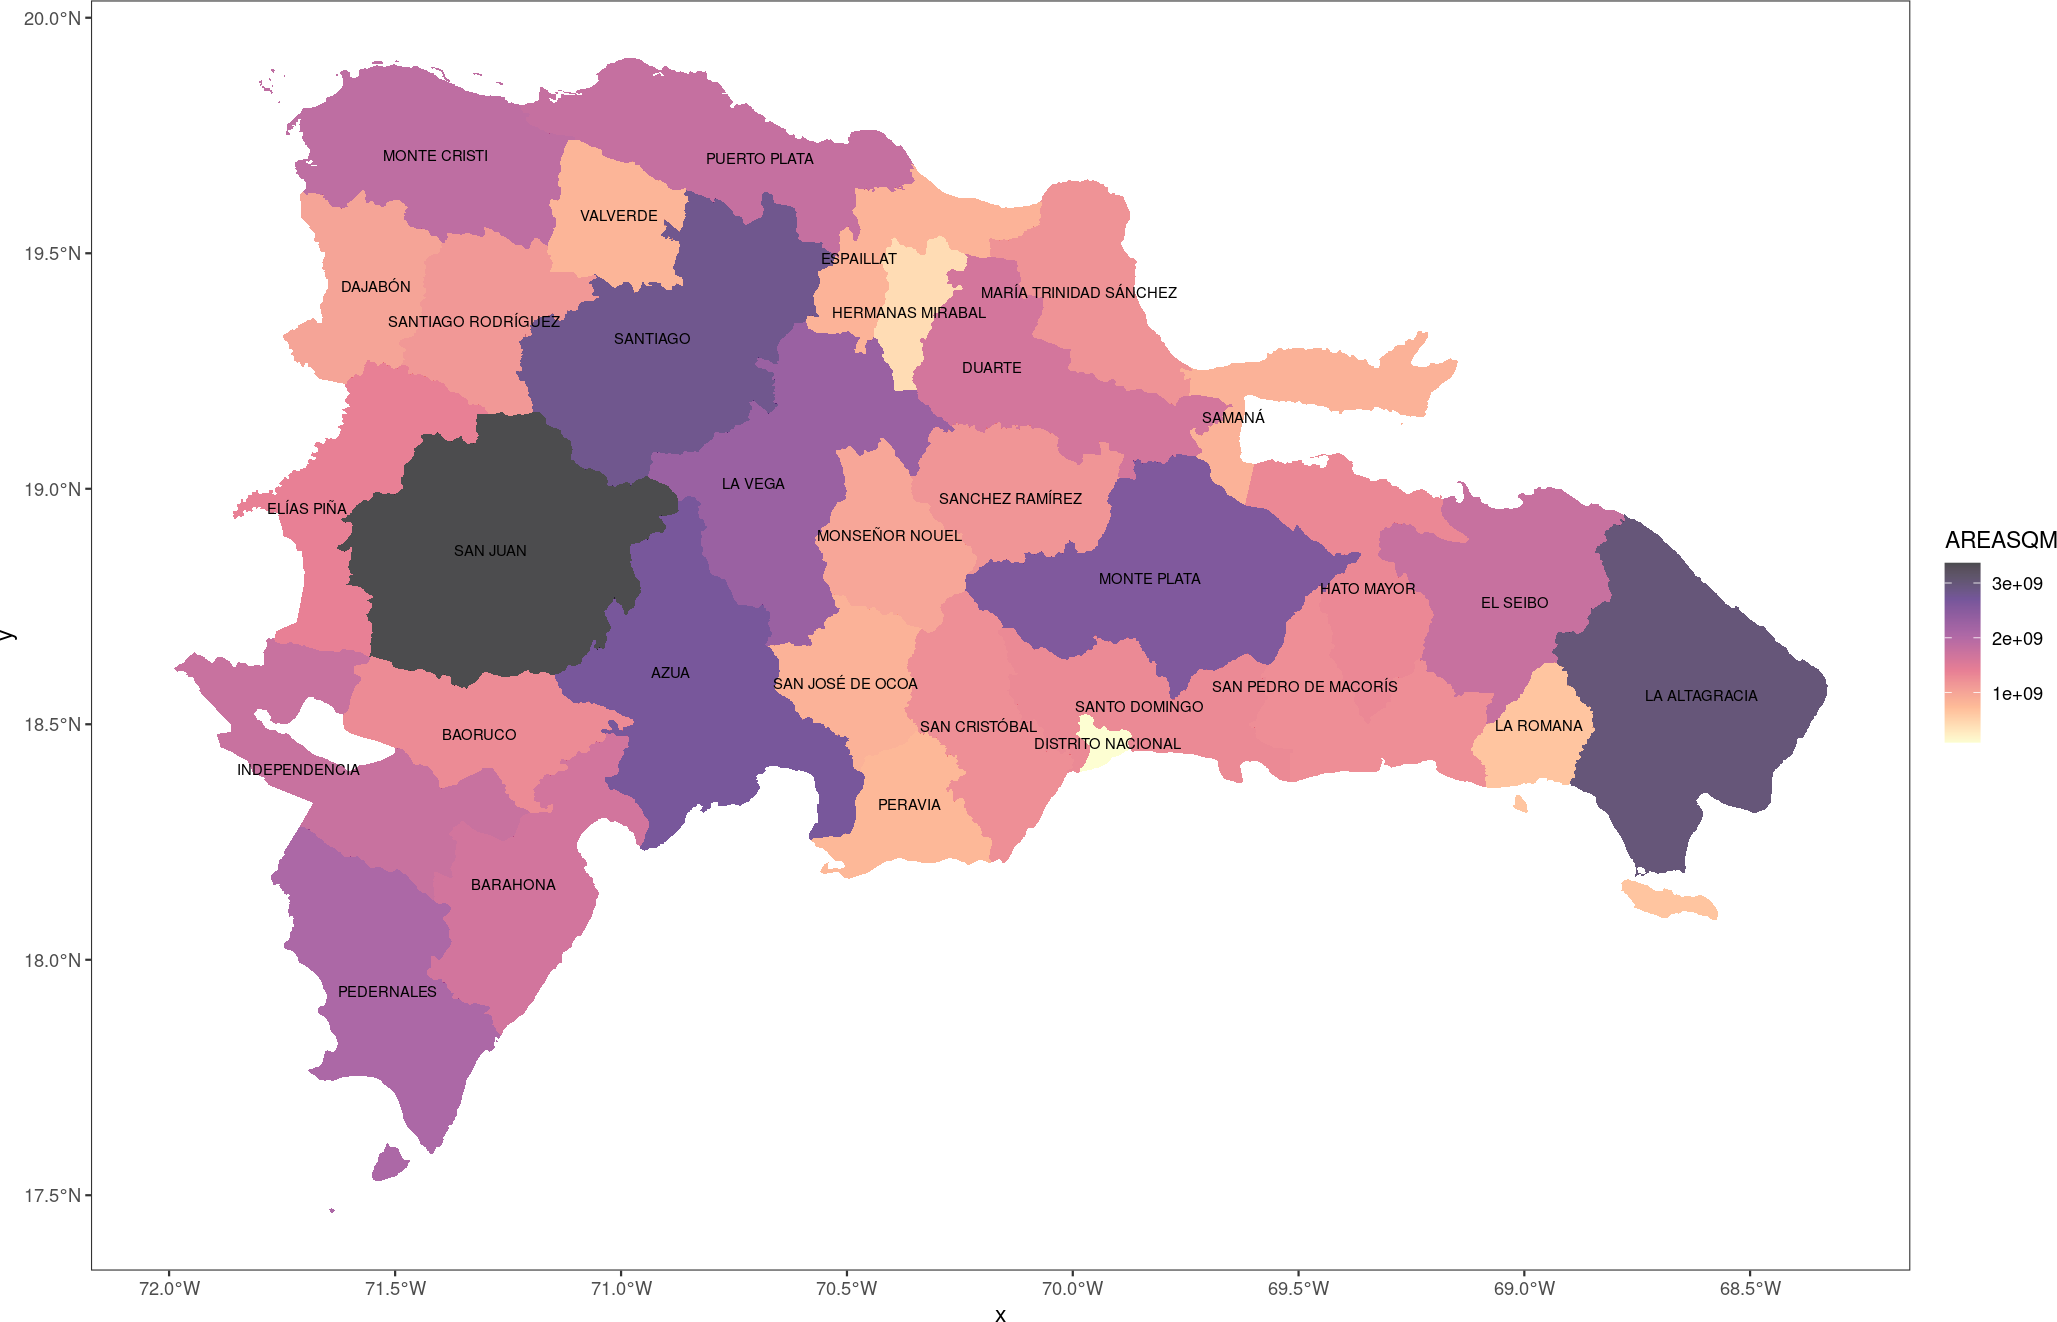
\includegraphics{img/data-download-preparation-eda/administrative-1} \end{center}

\begin{Shaded}
\begin{Highlighting}[]
\NormalTok{mun }\OtherTok{\textless{}{-}} \FunctionTok{st\_read}\NormalTok{(admpath, }\StringTok{\textquotesingle{}MUNCenso2010\textquotesingle{}}\NormalTok{, }\AttributeTok{quiet =}\NormalTok{ T)}
\NormalTok{mun}
\DocumentationTok{\#\# Simple feature collection with 155 features and 5 fields}
\DocumentationTok{\#\# Geometry type: MULTIPOLYGON}
\DocumentationTok{\#\# Dimension:     XY}
\DocumentationTok{\#\# Bounding box:  xmin: 182215.8 ymin: 1933532 xmax: 571365.3 ymax: 2205216}
\DocumentationTok{\#\# Projected CRS: WGS 84 / UTM zone 19N}
\DocumentationTok{\#\# First 10 features:}
\DocumentationTok{\#\#    PROV MUN REG               TOPONIMIA ENLACE                           geom}
\DocumentationTok{\#\# 1    01  01  10 SANTO DOMINGO DE GUZMÁN 100101 MULTIPOLYGON (((405218.1 20...}
\DocumentationTok{\#\# 2    02  01  05                    AZUA 050201 MULTIPOLYGON (((319065.3 20...}
\DocumentationTok{\#\# 3    02  02  05             LAS CHARCAS 050202 MULTIPOLYGON (((341415.3 20...}
\DocumentationTok{\#\# 4    02  03  05    LAS YAYAS DE VIAJAMA 050203 MULTIPOLYGON (((304058.1 20...}
\DocumentationTok{\#\# 5    02  04  05         PADRE LAS CASAS 050204 MULTIPOLYGON (((312890.8 20...}
\DocumentationTok{\#\# 6    02  05  05                 PERALTA 050205 MULTIPOLYGON (((317370.6 20...}
\DocumentationTok{\#\# 7    02  06  05            SABANA YEGUA 050206 MULTIPOLYGON (((306745.8 20...}
\DocumentationTok{\#\# 8    02  07  05            PUEBLO VIEJO 050207 MULTIPOLYGON (((310447.9 20...}
\DocumentationTok{\#\# 9    02  08  05           TÁBARA ARRIBA 050208 MULTIPOLYGON (((306556.7 20...}
\DocumentationTok{\#\# 10   02  09  05                GUAYABAL 050209 MULTIPOLYGON (((322129.5 20...}
\NormalTok{mun }\OtherTok{\textless{}{-}}\NormalTok{ mun }\SpecialCharTok{\%\textgreater{}\%} \FunctionTok{mutate}\NormalTok{(}\AttributeTok{AREASQM =} \FunctionTok{st\_area}\NormalTok{(geom) }\SpecialCharTok{\%\textgreater{}\%}\NormalTok{ units}\SpecialCharTok{::}\FunctionTok{drop\_units}\NormalTok{())}
\NormalTok{mun }\SpecialCharTok{\%\textgreater{}\%}\NormalTok{ ggplot }\SpecialCharTok{+} \FunctionTok{aes}\NormalTok{(}\AttributeTok{fill=}\NormalTok{AREASQM, }\AttributeTok{label =}\NormalTok{ TOPONIMIA) }\SpecialCharTok{+}
  \FunctionTok{geom\_sf}\NormalTok{(}\AttributeTok{color=}\StringTok{\textquotesingle{}transparent\textquotesingle{}}\NormalTok{) }\SpecialCharTok{+}
  \FunctionTok{scale\_fill\_viridis\_c}\NormalTok{(}\AttributeTok{option =} \StringTok{\textquotesingle{}magma\textquotesingle{}}\NormalTok{, }\AttributeTok{direction =} \SpecialCharTok{{-}}\DecValTok{1}\NormalTok{, }\AttributeTok{alpha =} \FloatTok{0.7}\NormalTok{) }\SpecialCharTok{+}
  \FunctionTok{geom\_sf\_text}\NormalTok{(}\AttributeTok{size =} \DecValTok{2}\NormalTok{) }\SpecialCharTok{+}
  \FunctionTok{theme\_bw}\NormalTok{() }\SpecialCharTok{+}
  \FunctionTok{theme}\NormalTok{(}\AttributeTok{panel.grid=}\FunctionTok{element\_blank}\NormalTok{())}
\end{Highlighting}
\end{Shaded}

\begin{center}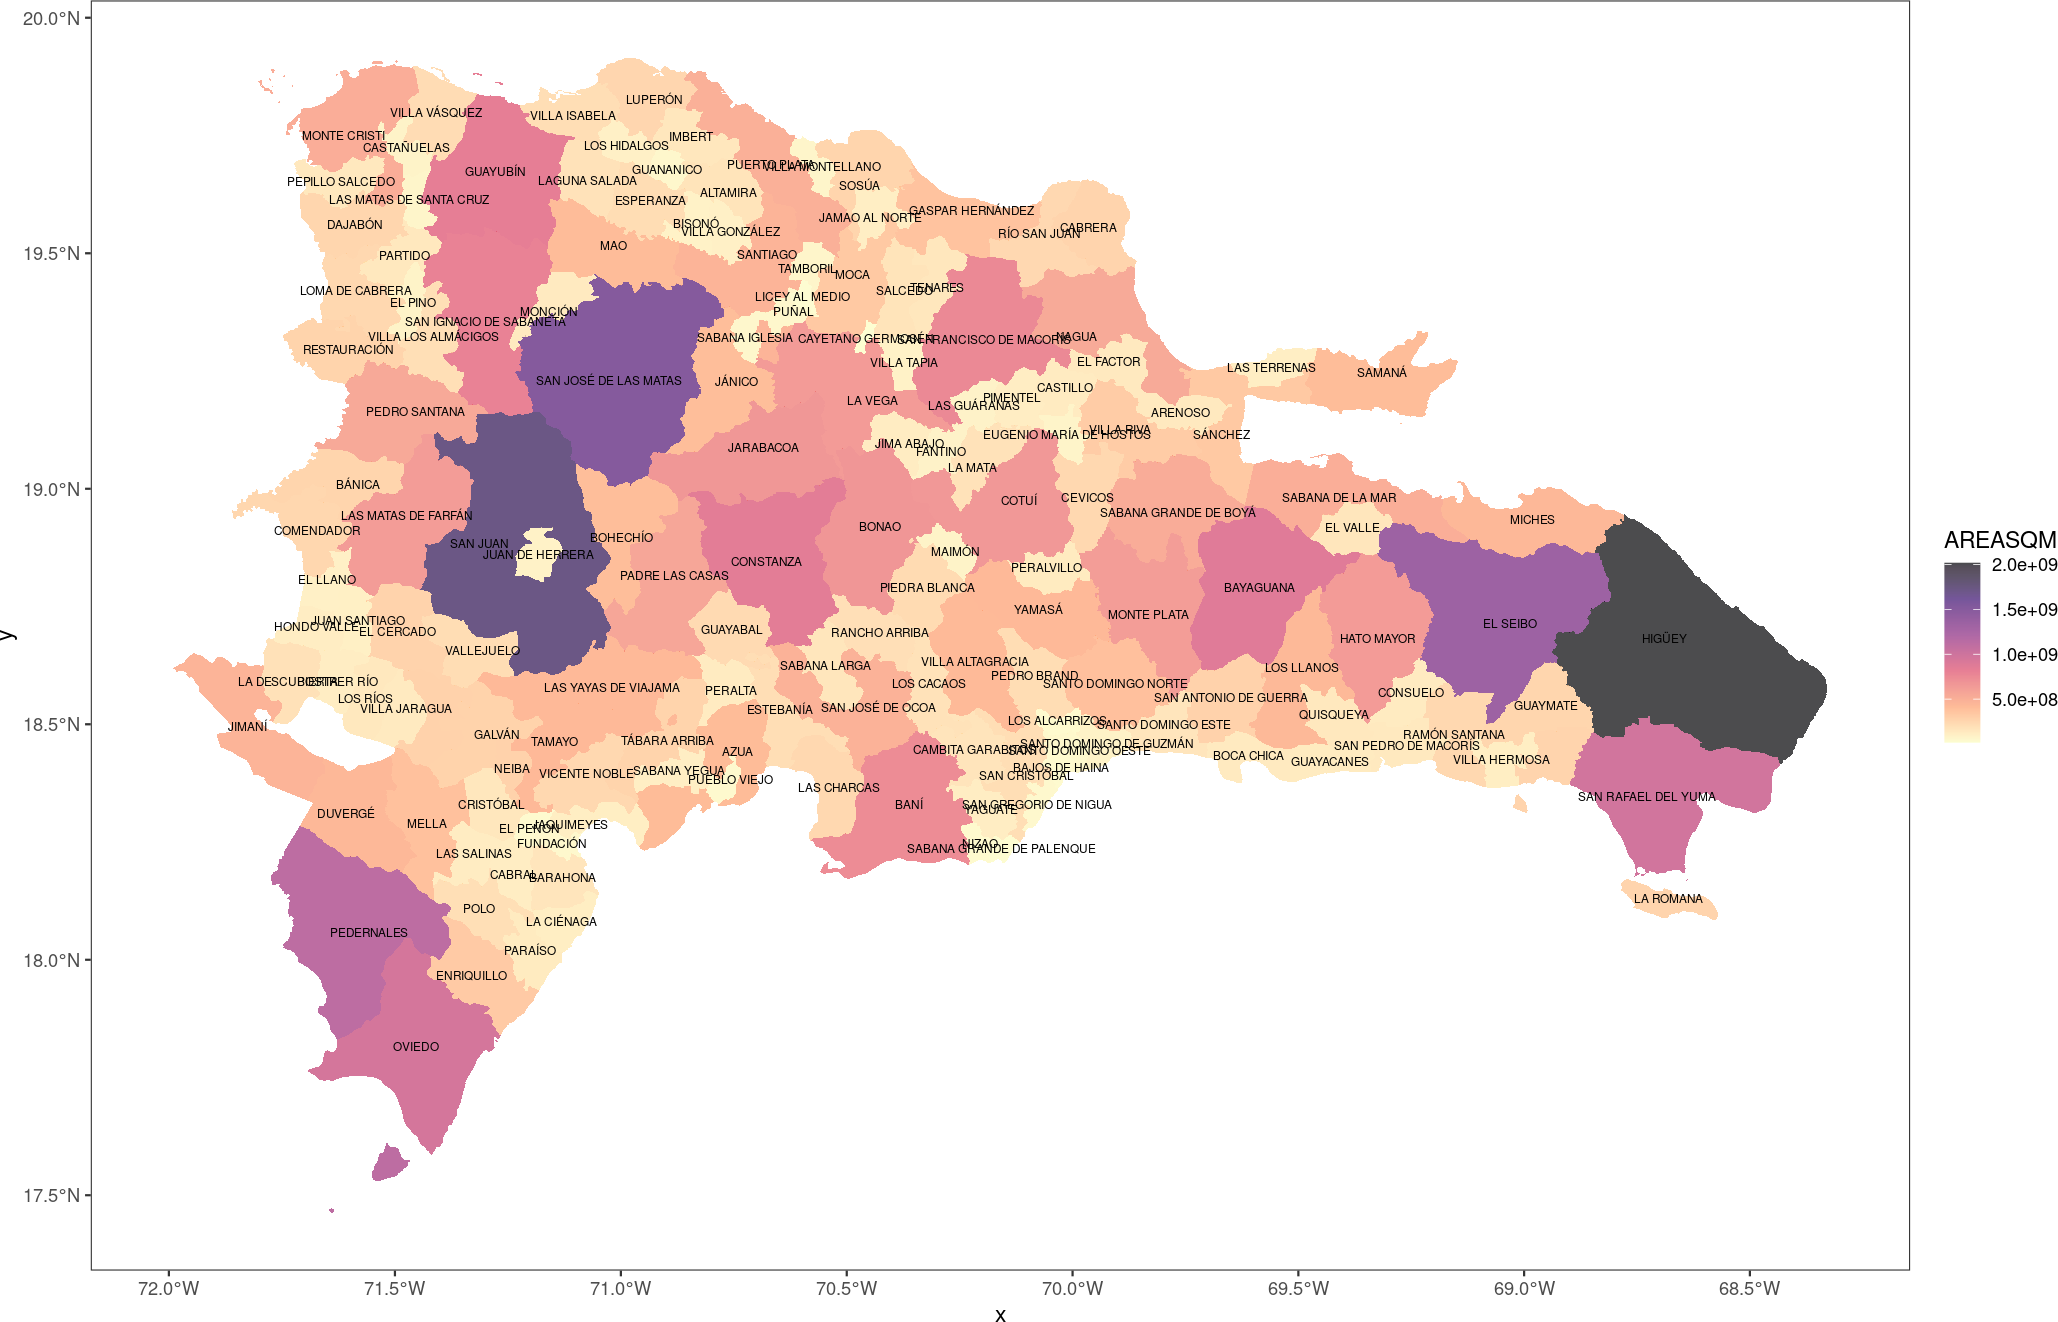
\includegraphics{img/data-download-preparation-eda/administrative-2} \end{center}

\hypertarget{protected-areas}{%
\subsubsection{Protected areas}\label{protected-areas}}

Source: UNEP-WCMC and IUCN (October 2021)

\begin{Shaded}
\begin{Highlighting}[]
\NormalTok{papath }\OtherTok{\textless{}{-}} \StringTok{\textquotesingle{}data/protected\_areas/protected{-}areas.gpkg\textquotesingle{}}
\FunctionTok{st\_layers}\NormalTok{(papath)}
\DocumentationTok{\#\# Driver: GPKG }
\DocumentationTok{\#\# Available layers:}
\DocumentationTok{\#\#        layer\_name geometry\_type features fields}
\DocumentationTok{\#\# 1 Protected Areas Multi Polygon      143     30}
\NormalTok{pa }\OtherTok{\textless{}{-}} \FunctionTok{st\_read}\NormalTok{(papath, }\StringTok{\textquotesingle{}Protected Areas\textquotesingle{}}\NormalTok{, }\AttributeTok{quiet =}\NormalTok{ T) }\SpecialCharTok{\%\textgreater{}\%} \FunctionTok{st\_transform}\NormalTok{(}\DecValTok{32619}\NormalTok{)}
\NormalTok{pa}
\DocumentationTok{\#\# Simple feature collection with 143 features and 30 fields}
\DocumentationTok{\#\# Geometry type: MULTIPOLYGON}
\DocumentationTok{\#\# Dimension:     XY}
\DocumentationTok{\#\# Bounding box:  xmin: 185574.6 ymin: 1893434 xmax: 622910.8 ymax: 2333086}
\DocumentationTok{\#\# Projected CRS: WGS 84 / UTM zone 19N}
\DocumentationTok{\#\# First 10 features:}
\DocumentationTok{\#\#    WDPAID WDPA\_PID PA\_DEF                   NAME              ORIG\_NAME}
\DocumentationTok{\#\# 1     180      180      1  Cotubanamá (Del Este)  Cotubanamá (Del Este)}
\DocumentationTok{\#\# 2     181      181      1           Los Haitises           Los Haitises}
\DocumentationTok{\#\# 3    6673     6673      1                Jaragua                Jaragua}
\DocumentationTok{\#\# 4    6674     6674      1 Submarino Monte Cristi Submarino Monte Cristi}
\DocumentationTok{\#\# 5    6675     6675      1     Sierra de Bahoruco     Sierra de Bahoruco}
\DocumentationTok{\#\# 6  478066   478066      1               Alto bao               Alto bao}
\DocumentationTok{\#\# 7  478067   478067      1               Alto Mao               Alto Mao}
\DocumentationTok{\#\# 8  478068   478068      1       Armando Bermúdez       Armando Bermúdez}
\DocumentationTok{\#\# 9  478069   478069      1            Arroyo Cano            Arroyo Cano}
\DocumentationTok{\#\# 10 478070   478070      1       Bahia de Luperón       Bahia de Luperón}
\DocumentationTok{\#\#                        DESIG            DESIG\_ENG DESIG\_TYPE IUCN\_CAT}
\DocumentationTok{\#\# 1            Parque Nacional        National Park   National       II}
\DocumentationTok{\#\# 2            Parque Nacional        National Park   National       II}
\DocumentationTok{\#\# 3            Parque Nacional        National Park   National       II}
\DocumentationTok{\#\# 4  Parque Nacional Submarino Marine National Park   National       II}
\DocumentationTok{\#\# 5            Parque Nacional        National Park   National       II}
\DocumentationTok{\#\# 6           Reserva Forestal       Forest Reserve   National        V}
\DocumentationTok{\#\# 7           Reserva Forestal       Forest Reserve   National        V}
\DocumentationTok{\#\# 8            Parque Nacional        National Park   National       II}
\DocumentationTok{\#\# 9           Reserva Forestal       Forest Reserve   National        V}
\DocumentationTok{\#\# 10 Refugio de Vida Silvestre      Wildlife Refuge   National       IV}
\DocumentationTok{\#\#          INT\_CRIT MARINE REP\_M\_AREA  GIS\_M\_AREA REP\_AREA   GIS\_AREA}
\DocumentationTok{\#\# 1  Not Applicable      1     381.78 378.5932313  796.405  801.33295}
\DocumentationTok{\#\# 2  Not Applicable      0       0.00   0.5377948  631.681  635.48169}
\DocumentationTok{\#\# 3  Not Applicable      1     829.18 817.7824560 1535.470 1541.74197}
\DocumentationTok{\#\# 4  Not Applicable      2     246.45 238.2627059  246.450  246.28055}
\DocumentationTok{\#\# 5  Not Applicable      0       0.00   0.0000000 1091.770 1097.13371}
\DocumentationTok{\#\# 6  Not Applicable      0       0.00   0.0000000  307.270  263.91396}
\DocumentationTok{\#\# 7  Not Applicable      0       0.00   0.0000000  457.050  211.08661}
\DocumentationTok{\#\# 8  Not Applicable      0       0.00   0.0000000  802.550  806.46533}
\DocumentationTok{\#\# 9  Not Applicable      0       0.00   0.0000000   23.900   24.01876}
\DocumentationTok{\#\# 10 Not Applicable      1       5.49   5.0876446   18.700   18.77749}
\DocumentationTok{\#\#           NO\_TAKE NO\_TK\_AREA     STATUS STATUS\_YR}
\DocumentationTok{\#\# 1    Not Reported          0 Designated      2014}
\DocumentationTok{\#\# 2  Not Applicable          0 Designated      2004}
\DocumentationTok{\#\# 3    Not Reported          0 Designated      2004}
\DocumentationTok{\#\# 4    Not Reported          0 Designated      2004}
\DocumentationTok{\#\# 5  Not Applicable          0 Designated      2004}
\DocumentationTok{\#\# 6  Not Applicable          0 Designated      2004}
\DocumentationTok{\#\# 7  Not Applicable          0 Designated      2004}
\DocumentationTok{\#\# 8  Not Applicable          0 Designated      2004}
\DocumentationTok{\#\# 9  Not Applicable          0 Designated      2004}
\DocumentationTok{\#\# 10   Not Reported          0 Designated      2004}
\DocumentationTok{\#\#                                  GOV\_TYPE     OWN\_TYPE    MANG\_AUTH MANG\_PLAN}
\DocumentationTok{\#\# 1  Federal or national ministry or agency Not Reported Not Reported Yes, 2013}
\DocumentationTok{\#\# 2  Federal or national ministry or agency Not Reported Not Reported Yes, 2013}
\DocumentationTok{\#\# 3  Federal or national ministry or agency Not Reported Not Reported Yes, 2015}
\DocumentationTok{\#\# 4  Federal or national ministry or agency Not Reported Not Reported        No}
\DocumentationTok{\#\# 5  Federal or national ministry or agency Not Reported Not Reported Yes, 2007}
\DocumentationTok{\#\# 6  Federal or national ministry or agency Not Reported Not Reported        No}
\DocumentationTok{\#\# 7  Federal or national ministry or agency Not Reported Not Reported        No}
\DocumentationTok{\#\# 8  Federal or national ministry or agency Not Reported Not Reported Yes, 2005}
\DocumentationTok{\#\# 9  Federal or national ministry or agency Not Reported Not Reported        No}
\DocumentationTok{\#\# 10 Federal or national ministry or agency Not Reported Not Reported        No}
\DocumentationTok{\#\#             VERIF METADATAID      SUB\_LOC PARENT\_ISO ISO3      SUPP\_INFO}
\DocumentationTok{\#\# 1  State Verified        830 Not Reported        DOM  DOM Not Applicable}
\DocumentationTok{\#\# 2  State Verified        830 Not Reported        DOM  DOM Not Applicable}
\DocumentationTok{\#\# 3  State Verified        830 Not Reported        DOM  DOM Not Applicable}
\DocumentationTok{\#\# 4  State Verified        830 Not Reported        DOM  DOM Not Applicable}
\DocumentationTok{\#\# 5  State Verified        830        DO{-}16        DOM  DOM Not Applicable}
\DocumentationTok{\#\# 6  State Verified        830        DO{-}25        DOM  DOM Not Applicable}
\DocumentationTok{\#\# 7  State Verified        830 Not Reported        DOM  DOM Not Applicable}
\DocumentationTok{\#\# 8  State Verified        830        DO{-}25        DOM  DOM Not Applicable}
\DocumentationTok{\#\# 9  State Verified        830        DO{-}02        DOM  DOM Not Applicable}
\DocumentationTok{\#\# 10 State Verified        830 Not Reported        DOM  DOM Not Applicable}
\DocumentationTok{\#\#          CONS\_OBJ                           geom}
\DocumentationTok{\#\# 1  Not Applicable MULTIPOLYGON (((522048.1 20...}
\DocumentationTok{\#\# 2  Not Applicable MULTIPOLYGON (((397402.4 21...}
\DocumentationTok{\#\# 3  Not Applicable MULTIPOLYGON (((217347 2001...}
\DocumentationTok{\#\# 4  Not Applicable MULTIPOLYGON (((243475.9 22...}
\DocumentationTok{\#\# 5  Not Applicable MULTIPOLYGON (((232865.5 20...}
\DocumentationTok{\#\# 6  Not Applicable MULTIPOLYGON (((287355.2 21...}
\DocumentationTok{\#\# 7  Not Applicable MULTIPOLYGON (((253093.5 21...}
\DocumentationTok{\#\# 8  Not Applicable MULTIPOLYGON (((251693.4 21...}
\DocumentationTok{\#\# 9  Not Applicable MULTIPOLYGON (((289126.3 20...}
\DocumentationTok{\#\# 10 Not Applicable MULTIPOLYGON (((300900.2 22...}
\NormalTok{pa }\OtherTok{\textless{}{-}}\NormalTok{ pa }\SpecialCharTok{\%\textgreater{}\%} \FunctionTok{mutate}\NormalTok{(}
  \AttributeTok{AREASQM =} \FunctionTok{st\_area}\NormalTok{(geom) }\SpecialCharTok{\%\textgreater{}\%}\NormalTok{ units}\SpecialCharTok{::}\FunctionTok{drop\_units}\NormalTok{(),}
  \AttributeTok{AREASQMLOG =} \FunctionTok{log}\NormalTok{(}\FunctionTok{st\_area}\NormalTok{(geom)) }\SpecialCharTok{\%\textgreater{}\%}\NormalTok{ units}\SpecialCharTok{::}\FunctionTok{drop\_units}\NormalTok{()}
\NormalTok{)}
\NormalTok{pa }\SpecialCharTok{\%\textgreater{}\%}\NormalTok{ ggplot }\SpecialCharTok{+} \FunctionTok{aes}\NormalTok{(}\AttributeTok{fill=}\NormalTok{AREASQMLOG) }\SpecialCharTok{+}
  \FunctionTok{geom\_sf}\NormalTok{(}\AttributeTok{data =}\NormalTok{ prov, }\AttributeTok{fill =} \StringTok{\textquotesingle{}transparent\textquotesingle{}}\NormalTok{, }\AttributeTok{lwd =} \FloatTok{0.1}\NormalTok{) }\SpecialCharTok{+}
  \FunctionTok{geom\_sf}\NormalTok{(}\AttributeTok{color=}\StringTok{\textquotesingle{}transparent\textquotesingle{}}\NormalTok{) }\SpecialCharTok{+}
  \FunctionTok{scale\_fill\_viridis\_c}\NormalTok{(}\AttributeTok{option =} \StringTok{\textquotesingle{}magma\textquotesingle{}}\NormalTok{, }\AttributeTok{direction =} \SpecialCharTok{{-}}\DecValTok{1}\NormalTok{, }\AttributeTok{alpha =} \FloatTok{0.7}\NormalTok{) }\SpecialCharTok{+}
  \FunctionTok{geom\_sf\_text}\NormalTok{(}\FunctionTok{aes}\NormalTok{(}\AttributeTok{label =}\NormalTok{ NAME), }\AttributeTok{size =} \DecValTok{2}\NormalTok{) }\SpecialCharTok{+}
  \FunctionTok{theme\_bw}\NormalTok{() }\SpecialCharTok{+}
  \FunctionTok{theme}\NormalTok{(}\AttributeTok{panel.grid=}\FunctionTok{element\_blank}\NormalTok{())}
\end{Highlighting}
\end{Shaded}

\begin{center}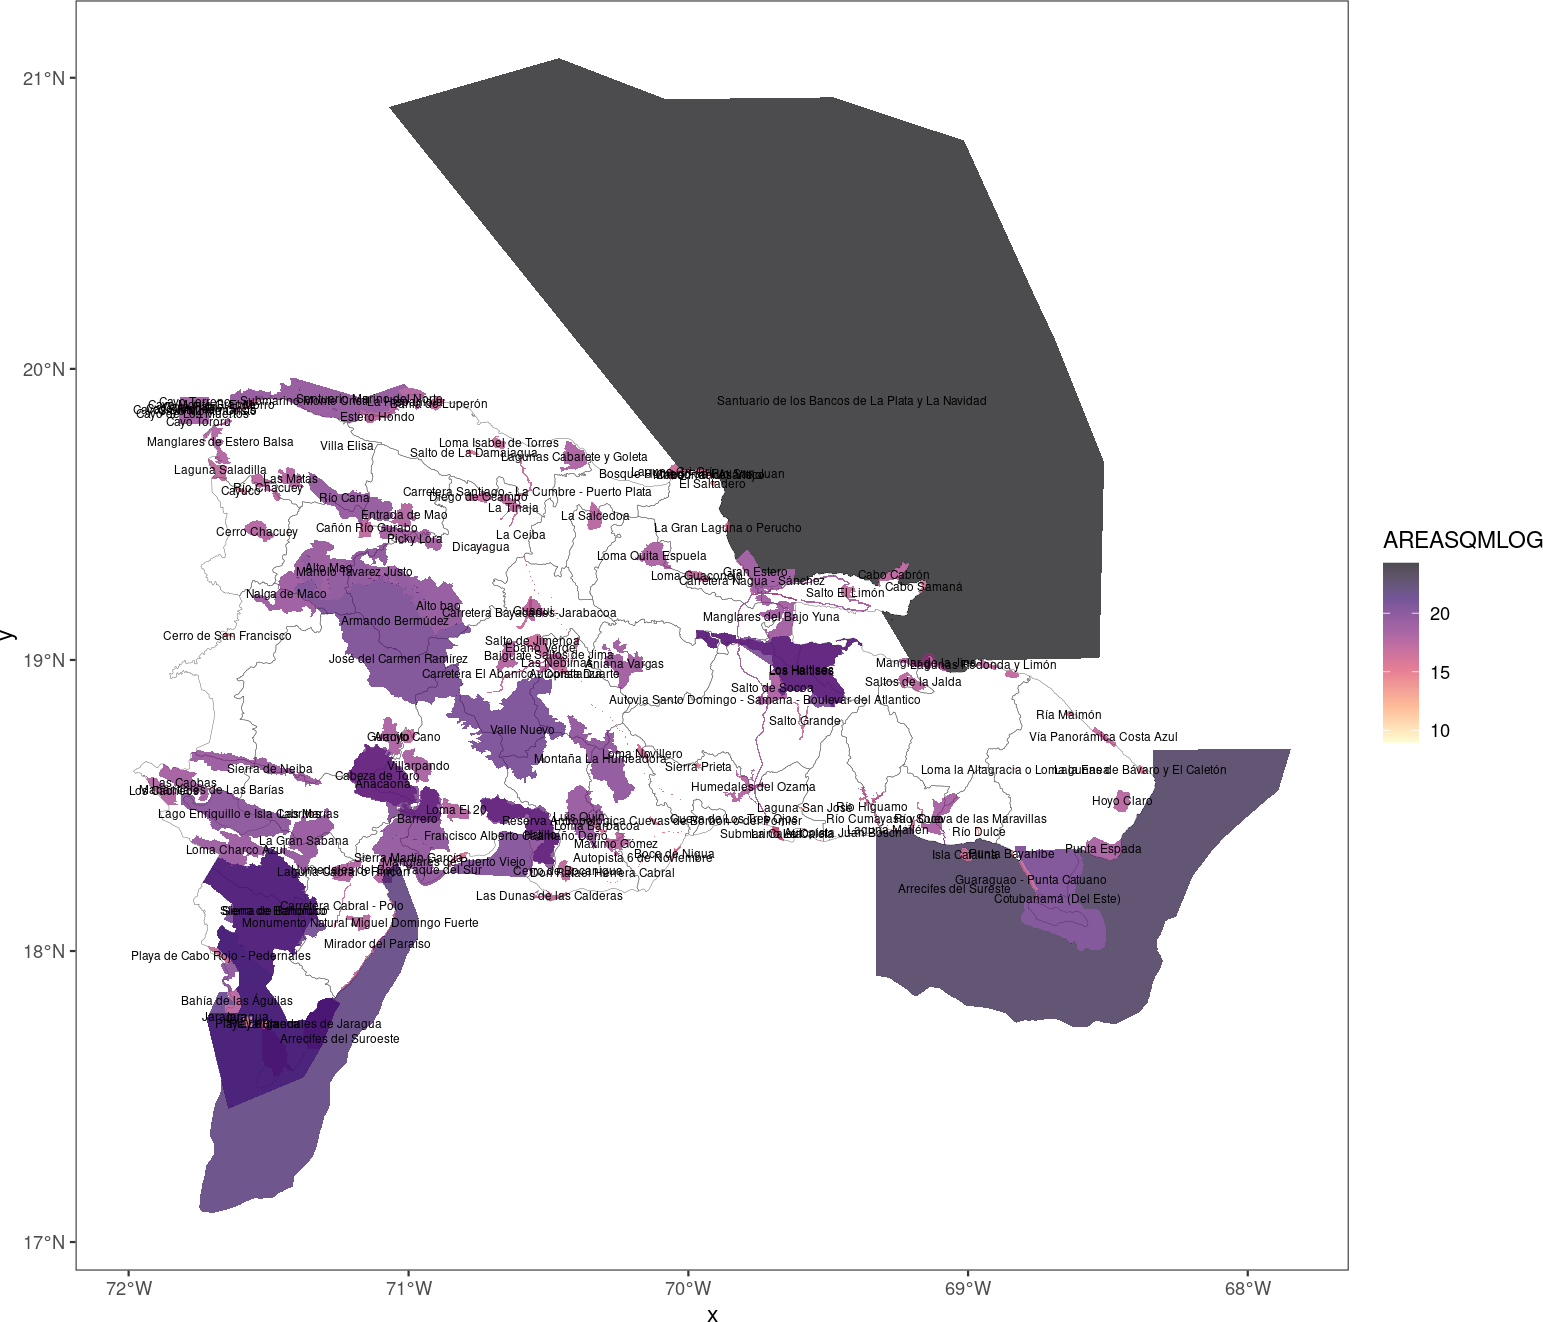
\includegraphics{img/data-download-preparation-eda/protected-areas-1} \end{center}

\hypertarget{cutline-for-cropping-raster-sources}{%
\subsection{Cutline for cropping raster
sources}\label{cutline-for-cropping-raster-sources}}

A cutline was generated using a shapefile from Oficina Nacional de
Estadística -ONE- (2015) as well as the datamask provided in Hansen et
al. (2013). In detail, the cutline was generated using the following
workflow: the international boundary between Haiti and the DR was
extracted as a polyline from Oficina Nacional de Estadística -ONE-
(2015); the remainder of the DR land area (water bodies excluded) was
extracted from a vectorized version of the datamask file from Hansen et
al. (2013); both layers were then joined together into a single cutline.
Afterwards, cropped and warped versions (e.g., onto EPSG:32619) of the
\texttt{datamask}, \texttt{lossyear}, \texttt{treecover} and
\texttt{gain} files were masked using the generated cutline.

\begin{Shaded}
\begin{Highlighting}[]
\FunctionTok{source}\NormalTok{(}\StringTok{\textquotesingle{}R/load{-}cutline.R\textquotesingle{}}\NormalTok{)}
\DocumentationTok{\#\# Reading layer \textasciigrave{}cutline\textquotesingle{} from data source }
\DocumentationTok{\#\#   \textasciigrave{}/home/jose/Documentos/git/forest{-}loss{-}fire{-}reproducible/out/cutline.geojson\textquotesingle{} }
\DocumentationTok{\#\#   using driver \textasciigrave{}GeoJSON\textquotesingle{}}
\DocumentationTok{\#\# Simple feature collection with 222 features and 2 fields}
\DocumentationTok{\#\# Geometry type: MULTIPOLYGON}
\DocumentationTok{\#\# Dimension:     XY}
\DocumentationTok{\#\# Bounding box:  xmin: 182239.3 ymin: 1933574 xmax: 571425.3 ymax: 2205219}
\DocumentationTok{\#\# Projected CRS: WGS 84 / UTM zone 19N}
\end{Highlighting}
\end{Shaded}

\hypertarget{download-and-prepare-forest-cover-and-forest-loss-data}{%
\section{Download and prepare forest cover and forest loss
data}\label{download-and-prepare-forest-cover-and-forest-loss-data}}

Using the
\texttt{R/original-script-used-to-download-and-prepare-forest-cover-and-forest-loss-data.R}
script many operations were accomplished to prepare the forest cover and
forest loss layers generated by Hansen et al., which included
downloading, mosaicking, cropping and clipping with the above mentioned
cutline. The resulting files were saved in the directory named
\texttt{out}, appending the suffix \texttt{\_crop} to each filename
(e.g.~\texttt{out/treecover2000\_crop.tif})

\hypertarget{tree-cover-forest-loss-and-fire-layers-importing-and-plotting}{%
\section{Tree cover, forest loss and fire layers: importing and
plotting}\label{tree-cover-forest-loss-and-fire-layers-importing-and-plotting}}

\hypertarget{tree-canopy-cover-of-year-2000}{%
\subsection{Tree canopy cover of year
2000}\label{tree-canopy-cover-of-year-2000}}

Set a percentage threshold above which tree-cover would be considered as
forest.

\begin{Shaded}
\begin{Highlighting}[]
\NormalTok{tc }\OtherTok{\textless{}{-}} \FunctionTok{raster}\NormalTok{(}\StringTok{\textquotesingle{}out/treecover2000\_crop.tif\textquotesingle{}}\NormalTok{)}
\FunctionTok{names}\NormalTok{(tc) }\OtherTok{\textless{}{-}} \StringTok{\textquotesingle{}TREECOVER2000\textquotesingle{}}
\FunctionTok{plot}\NormalTok{(}\FunctionTok{as\_Spatial}\NormalTok{(cline))}
\FunctionTok{plot}\NormalTok{(tc, }\AttributeTok{add =}\NormalTok{ T)}
\end{Highlighting}
\end{Shaded}

\begin{center}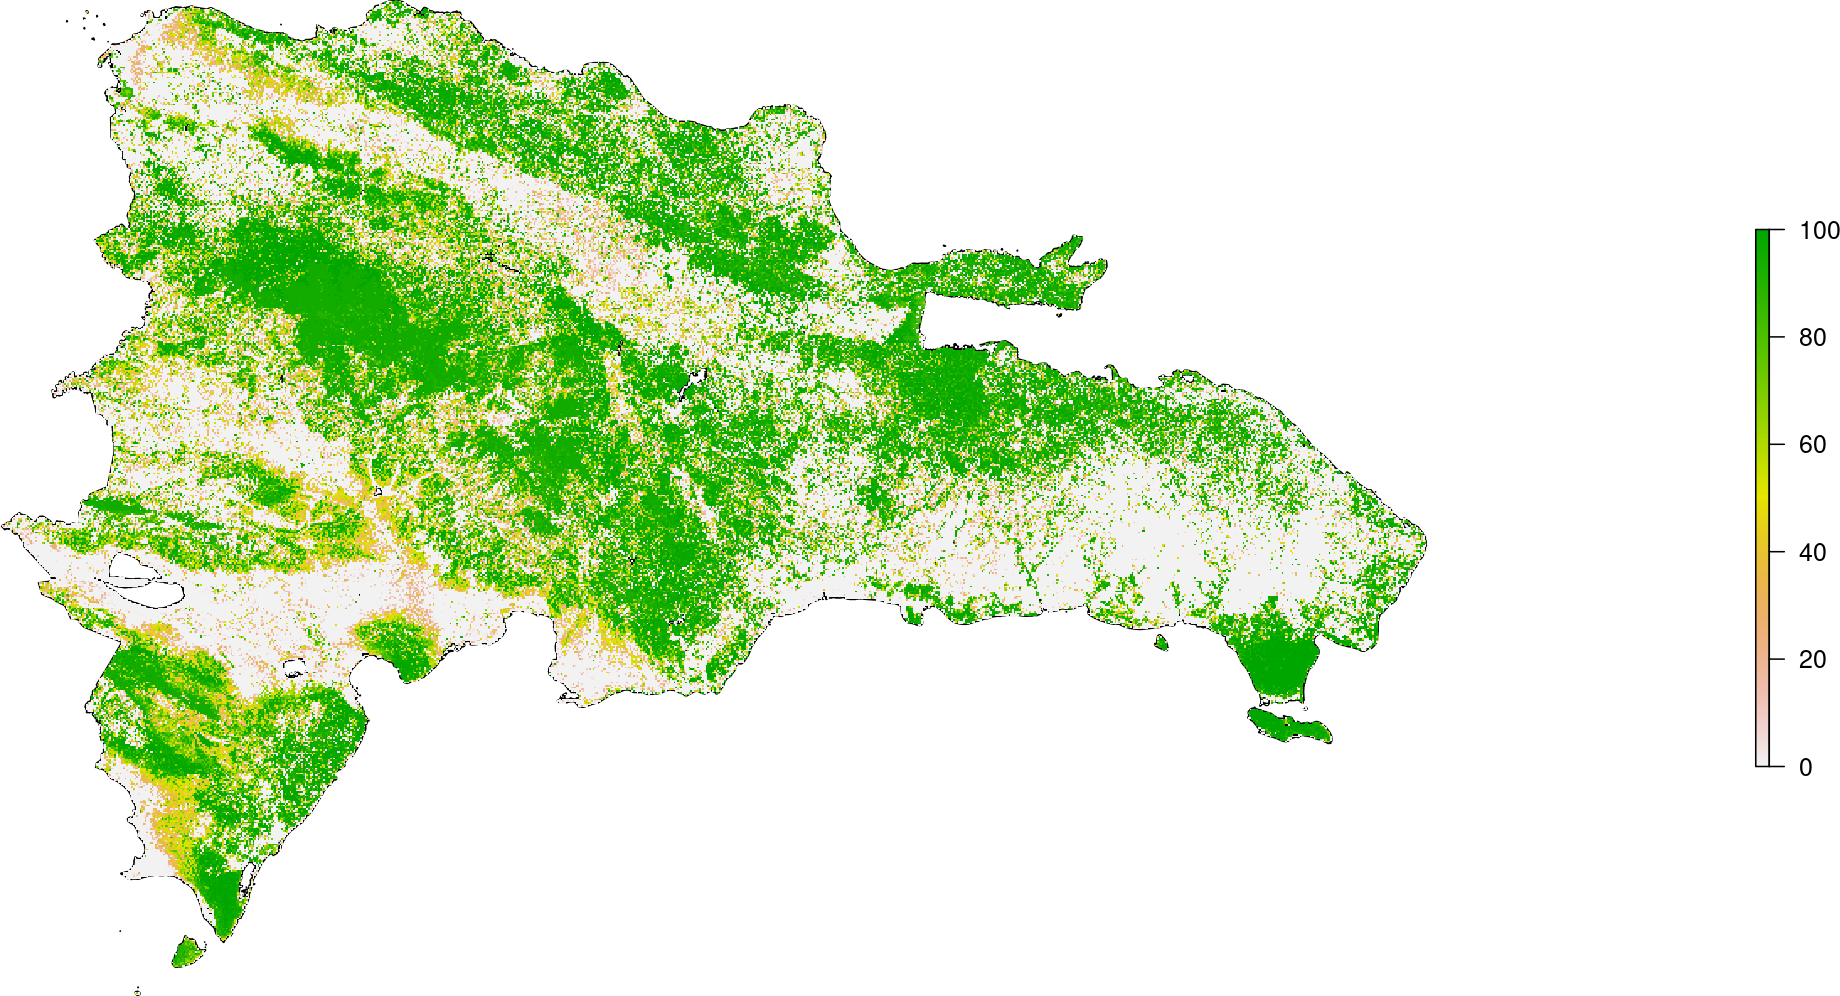
\includegraphics{img/data-download-preparation-eda/tree-canopy-cover-2000-nationwide-1} \end{center}

\begin{Shaded}
\begin{Highlighting}[]
\NormalTok{pctc }\OtherTok{\textless{}{-}} \DecValTok{25} \CommentTok{\#25\% or higher tree cover in year 2000 as a baseline is considered as "forest cover"}
\NormalTok{tcforzonal }\OtherTok{\textless{}{-}}\NormalTok{ tc}
\NormalTok{tcforzonal[tcforzonal }\SpecialCharTok{\textless{}}\NormalTok{ pctc] }\OtherTok{\textless{}{-}} \ConstantTok{NA}
\NormalTok{tcforzonal[tcforzonal }\SpecialCharTok{\textgreater{}=}\NormalTok{ pctc] }\OtherTok{\textless{}{-}} \DecValTok{1}
\FunctionTok{plot}\NormalTok{(}\FunctionTok{as\_Spatial}\NormalTok{(cline))}
\FunctionTok{plot}\NormalTok{(tcforzonal, }\AttributeTok{add =}\NormalTok{ T)}
\end{Highlighting}
\end{Shaded}

\begin{center}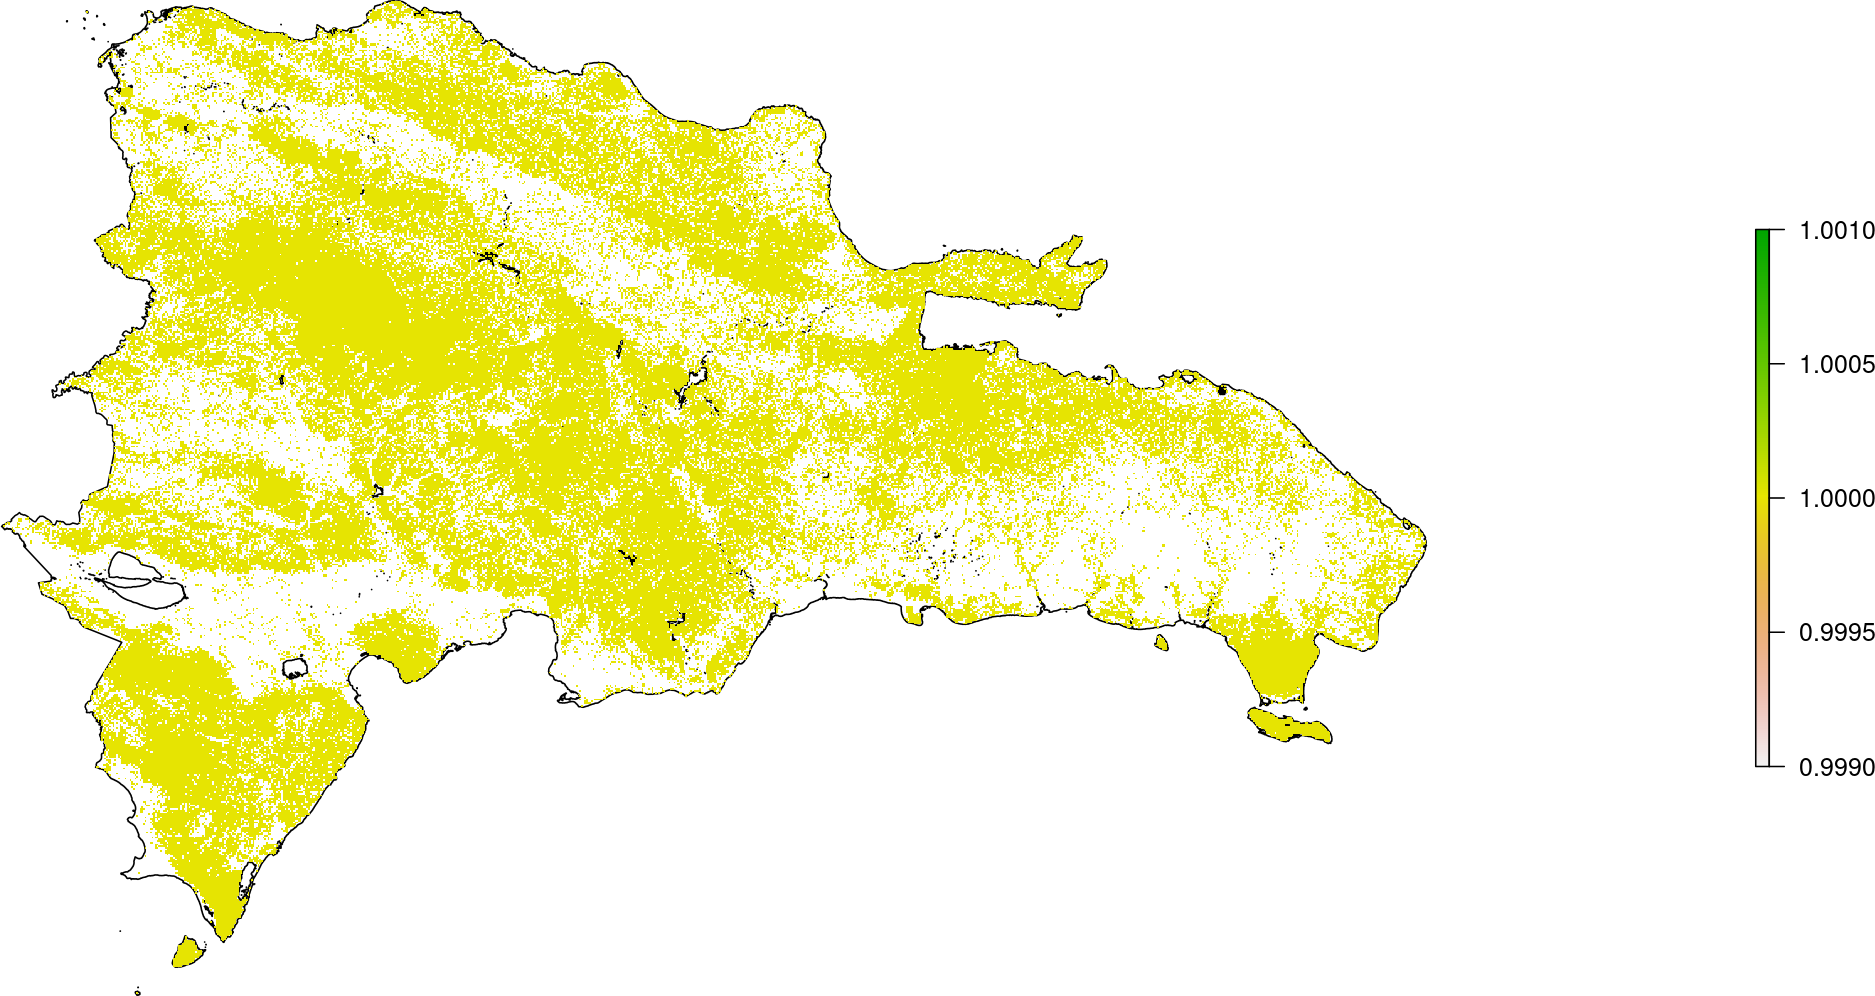
\includegraphics{img/data-download-preparation-eda/tree-canopy-cover-2000-nationwide-2} \end{center}

\hypertarget{year-of-gross-forest-cover-loss-2001-2018}{%
\subsection{Year of gross forest cover loss
(2001-2018)}\label{year-of-gross-forest-cover-loss-2001-2018}}

\begin{Shaded}
\begin{Highlighting}[]
\NormalTok{ly }\OtherTok{\textless{}{-}} \FunctionTok{raster}\NormalTok{(}\StringTok{\textquotesingle{}out/lossyear\_crop.tif\textquotesingle{}}\NormalTok{)}
\FunctionTok{names}\NormalTok{(ly) }\OtherTok{\textless{}{-}} \StringTok{\textquotesingle{}LOSSYEAR\textquotesingle{}}
\FunctionTok{plot}\NormalTok{(ly)}
\end{Highlighting}
\end{Shaded}

\begin{center}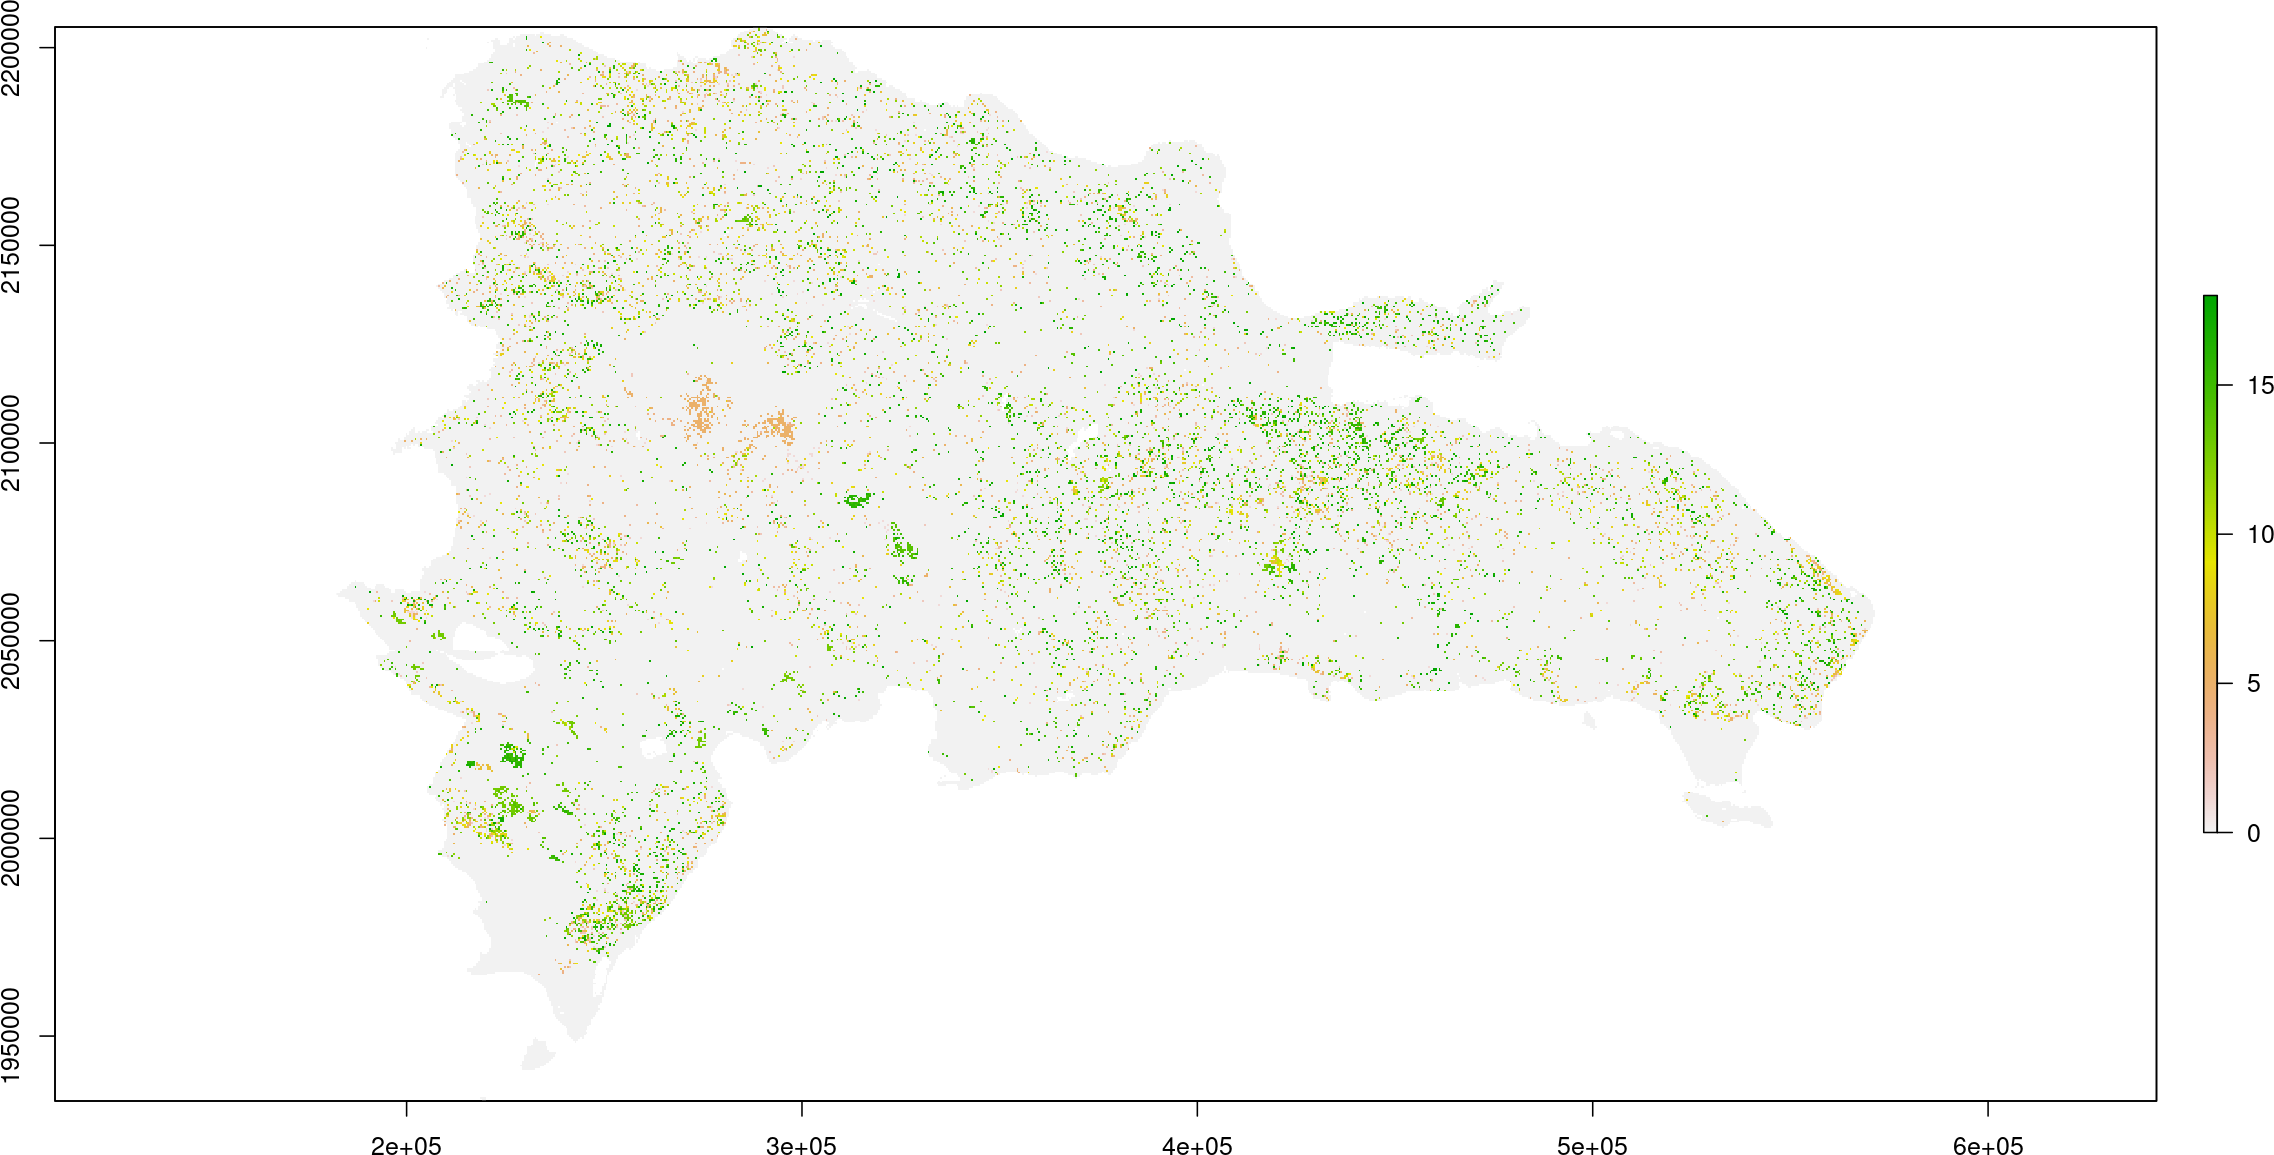
\includegraphics{img/data-download-preparation-eda/year-of-gross-forest-cover-loss-nationwide-1} \end{center}

\begin{Shaded}
\begin{Highlighting}[]
\NormalTok{lt }\OtherTok{\textless{}{-}}\NormalTok{ ly}
\NormalTok{lt[lt }\SpecialCharTok{\textgreater{}} \DecValTok{0}\NormalTok{] }\OtherTok{\textless{}{-}} \DecValTok{1}
\NormalTok{lt[lt }\SpecialCharTok{==} \DecValTok{0}\NormalTok{] }\OtherTok{\textless{}{-}} \ConstantTok{NA}
\FunctionTok{plot}\NormalTok{(}\FunctionTok{as\_Spatial}\NormalTok{(cline))}
\FunctionTok{plot}\NormalTok{(lt, }\AttributeTok{add =}\NormalTok{ T)}
\end{Highlighting}
\end{Shaded}

\begin{center}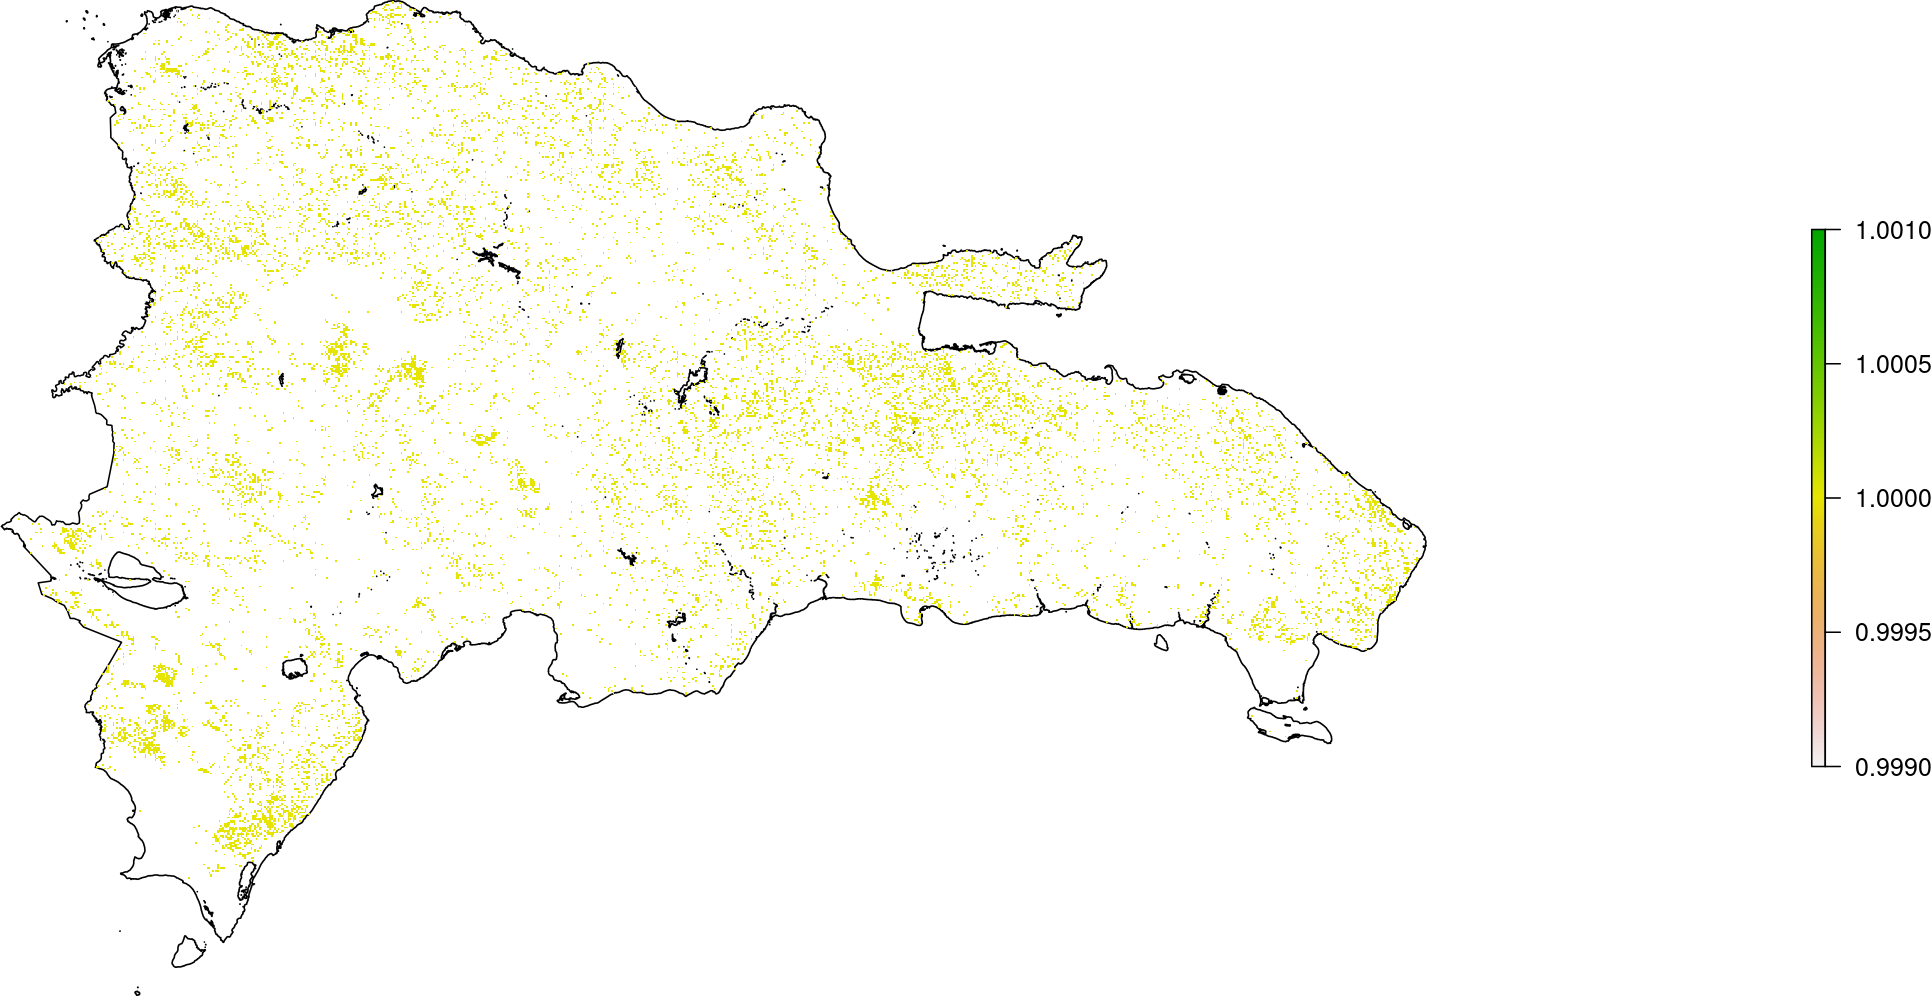
\includegraphics{img/data-download-preparation-eda/year-of-gross-forest-cover-loss-nationwide-2} \end{center}

\begin{Shaded}
\begin{Highlighting}[]
\NormalTok{lt1218 }\OtherTok{\textless{}{-}}\NormalTok{ ly}
\NormalTok{lt1218[ly }\SpecialCharTok{\textless{}=} \DecValTok{11}\NormalTok{] }\OtherTok{\textless{}{-}} \ConstantTok{NA}
\NormalTok{lt1218[ly }\SpecialCharTok{\textgreater{}} \DecValTok{11}\NormalTok{] }\OtherTok{\textless{}{-}} \DecValTok{1}
\FunctionTok{plot}\NormalTok{(}\FunctionTok{as\_Spatial}\NormalTok{(cline))}
\FunctionTok{plot}\NormalTok{(lt1218, }\AttributeTok{add =}\NormalTok{ T)}
\end{Highlighting}
\end{Shaded}

\begin{center}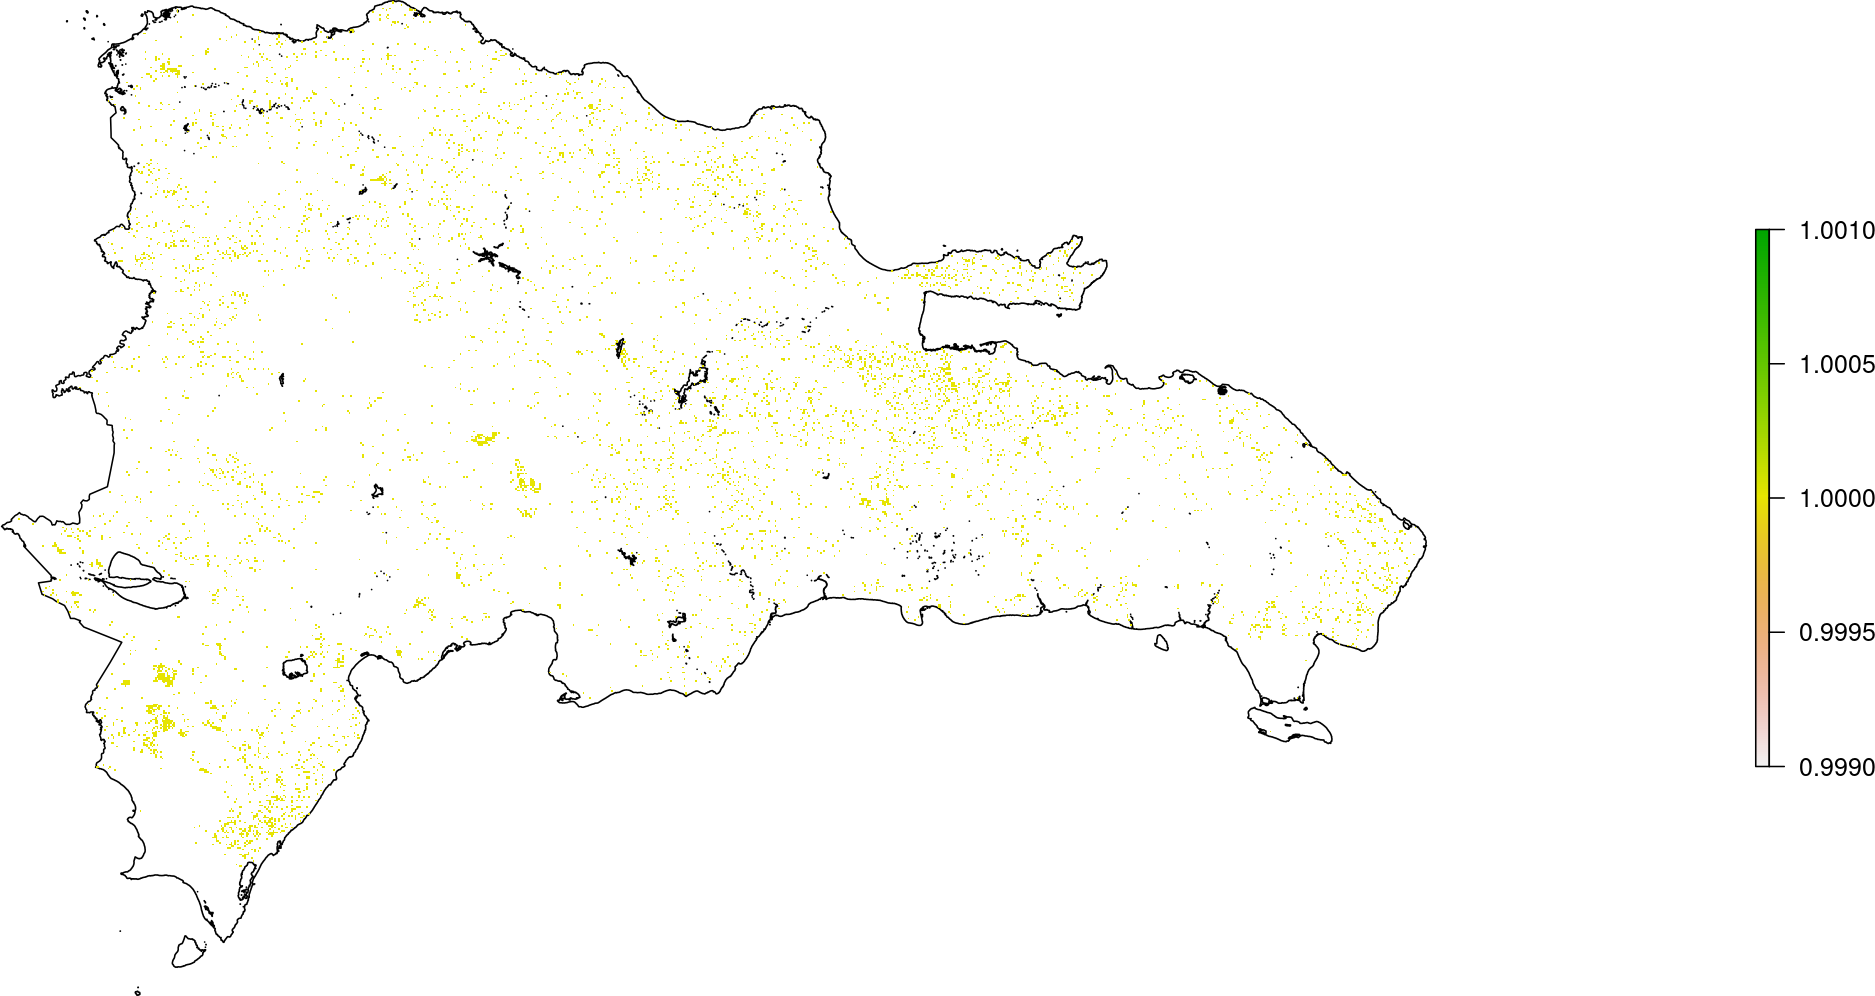
\includegraphics{img/data-download-preparation-eda/year-of-gross-forest-cover-loss-nationwide-3} \end{center}

\hypertarget{hotspotfire-layers-m6-and-v1-for-the-long-term-analytical-approach}{%
\subsection{Hotspot/fire layers (M6 and V1) for the long-term analytical
approach}\label{hotspotfire-layers-m6-and-v1-for-the-long-term-analytical-approach}}

The hotspot/fire/thermal anomalies layers (M6 and V1 datasets) were
created using the script
\texttt{R/original-script-used-to-create-the-hotspot-fire-layers-M6-and-V1-for-long-term-approach.R}.
This script was initially fed from a layer where thermal anomalies and
spontaneous fires from chimneys and landfills were manually removed from
each dataset, which were called ``noise-free versions of MODIS and VIIRS
datasets,'' respectively. Then, the script filtered out points falling
outside the mask (e.g.~outside forest cover), as well as points recorded
before 1-1-2001 and after 31-12-2018. Lastly, all points with a
confidence value of less than 30\% in the MODIS collection, as well as
those with a ``low confidence'' tag in the VIIRS collection, were
excluded from the dataset. For practical reasons, the fire layers are
simply loaded using the \texttt{readRDS} function as follows.

\begin{Shaded}
\begin{Highlighting}[]
\NormalTok{firesm6sel2 }\OtherTok{\textless{}{-}} \FunctionTok{st\_read}\NormalTok{(}\StringTok{\textquotesingle{}out/fire\_archive\_M6\_93308\_DR\_firesm6sel2.geojson\textquotesingle{}}\NormalTok{)}
\DocumentationTok{\#\# Reading layer \textasciigrave{}fire\_archive\_M6\_93308\_DR\_firesm6sel2\textquotesingle{} from data source }
\DocumentationTok{\#\#   \textasciigrave{}/home/jose/Documentos/git/forest{-}loss{-}fire{-}reproducible/out/fire\_archive\_M6\_93308\_DR\_firesm6sel2.geojson\textquotesingle{} }
\DocumentationTok{\#\#   using driver \textasciigrave{}GeoJSON\textquotesingle{}}
\DocumentationTok{\#\# Simple feature collection with 11861 features and 15 fields}
\DocumentationTok{\#\# Geometry type: POINT}
\DocumentationTok{\#\# Dimension:     XY}
\DocumentationTok{\#\# Bounding box:  xmin: 184698.8 ymin: 1964160 xmax: 568878.1 ymax: 2203503}
\DocumentationTok{\#\# Projected CRS: WGS 84 / UTM zone 19N}
\NormalTok{cline }\SpecialCharTok{\%\textgreater{}\%}\NormalTok{ as\_Spatial }\SpecialCharTok{\%\textgreater{}\%}\NormalTok{ plot}
\FunctionTok{plot}\NormalTok{(}\FunctionTok{as\_Spatial}\NormalTok{(firesm6sel2), }\AttributeTok{main =} \StringTok{"Thermal anomalies within forest M6"}\NormalTok{,}
     \AttributeTok{pch =} \DecValTok{1}\NormalTok{, }\AttributeTok{cex =} \FloatTok{0.1}\NormalTok{, }\AttributeTok{add =}\NormalTok{ T, }\AttributeTok{col =} \StringTok{\textquotesingle{}orange\textquotesingle{}}\NormalTok{)}
\end{Highlighting}
\end{Shaded}

\begin{center}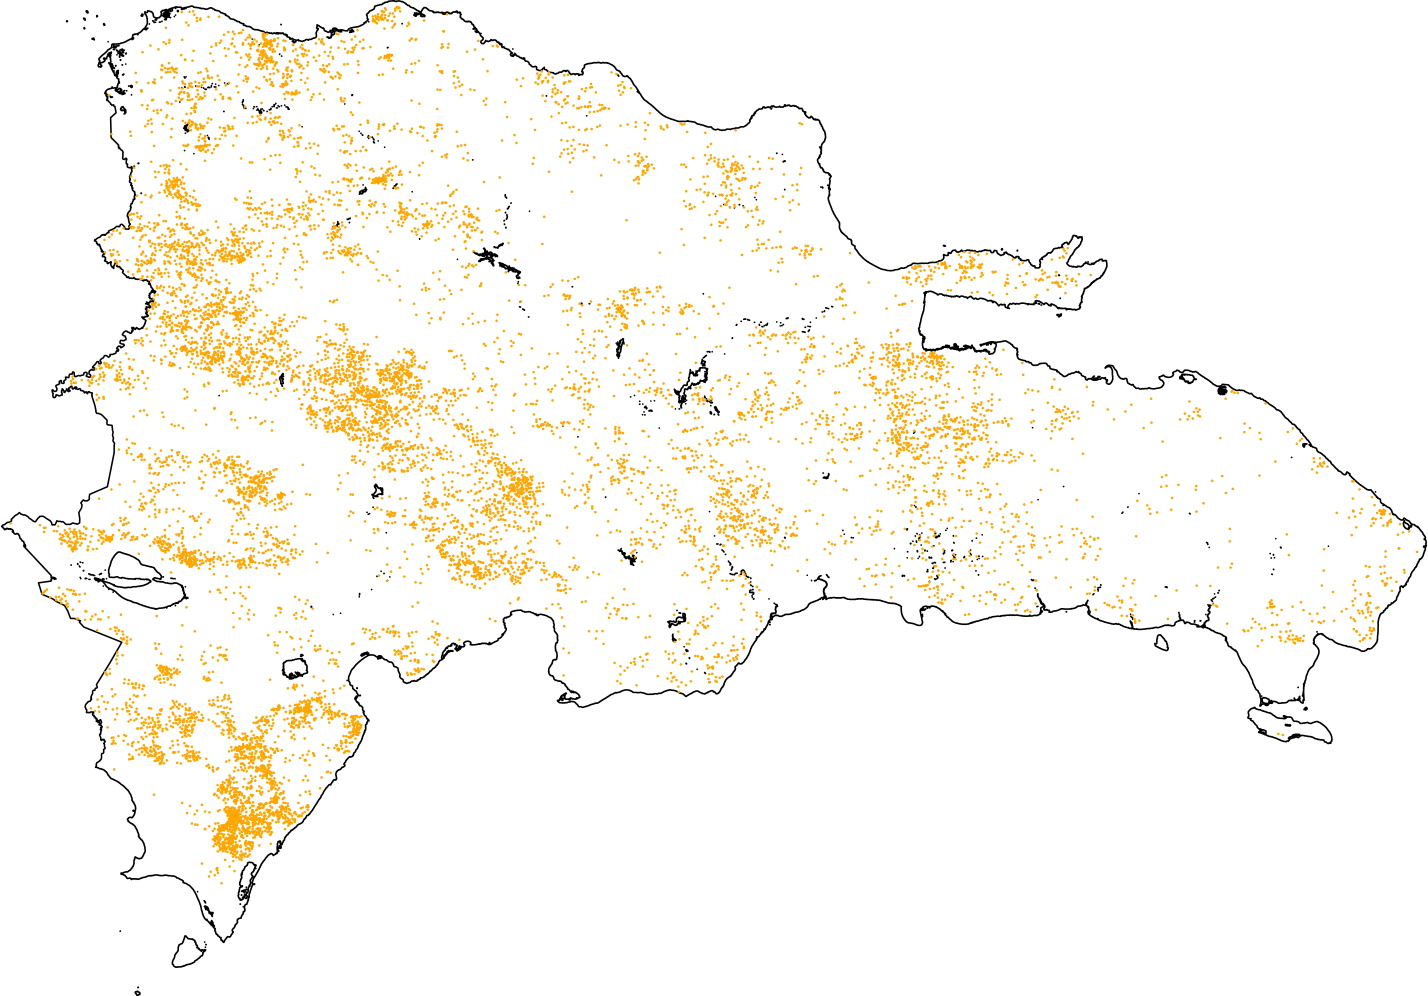
\includegraphics{img/data-download-preparation-eda/fires-m6-v1-sel2-1} \end{center}

\begin{Shaded}
\begin{Highlighting}[]
\NormalTok{firesv1sel2 }\OtherTok{\textless{}{-}} \FunctionTok{st\_read}\NormalTok{(}\StringTok{\textquotesingle{}out/fire\_archive\_V1\_93309\_DR\_firesv1sel2.geojson\textquotesingle{}}\NormalTok{)}
\DocumentationTok{\#\# Reading layer \textasciigrave{}fire\_archive\_V1\_93309\_DR\_firesv1sel2\textquotesingle{} from data source }
\DocumentationTok{\#\#   \textasciigrave{}/home/jose/Documentos/git/forest{-}loss{-}fire{-}reproducible/out/fire\_archive\_V1\_93309\_DR\_firesv1sel2.geojson\textquotesingle{} }
\DocumentationTok{\#\#   using driver \textasciigrave{}GeoJSON\textquotesingle{}}
\DocumentationTok{\#\# Simple feature collection with 25838 features and 14 fields}
\DocumentationTok{\#\# Geometry type: POINT}
\DocumentationTok{\#\# Dimension:     XY}
\DocumentationTok{\#\# Bounding box:  xmin: 184135.9 ymin: 1934167 xmax: 569069 ymax: 2204713}
\DocumentationTok{\#\# Projected CRS: WGS 84 / UTM zone 19N}
\NormalTok{cline }\SpecialCharTok{\%\textgreater{}\%}\NormalTok{ as\_Spatial }\SpecialCharTok{\%\textgreater{}\%}\NormalTok{ plot}
\FunctionTok{plot}\NormalTok{(}\FunctionTok{as\_Spatial}\NormalTok{(firesv1sel2), }\AttributeTok{main =} \StringTok{"Thermal anomalies within forest V1"}\NormalTok{,}
     \AttributeTok{pch =} \DecValTok{1}\NormalTok{, }\AttributeTok{cex =} \FloatTok{0.1}\NormalTok{, }\AttributeTok{add =}\NormalTok{ T, }\AttributeTok{col =} \StringTok{\textquotesingle{}orange\textquotesingle{}}\NormalTok{)}
\end{Highlighting}
\end{Shaded}

\begin{center}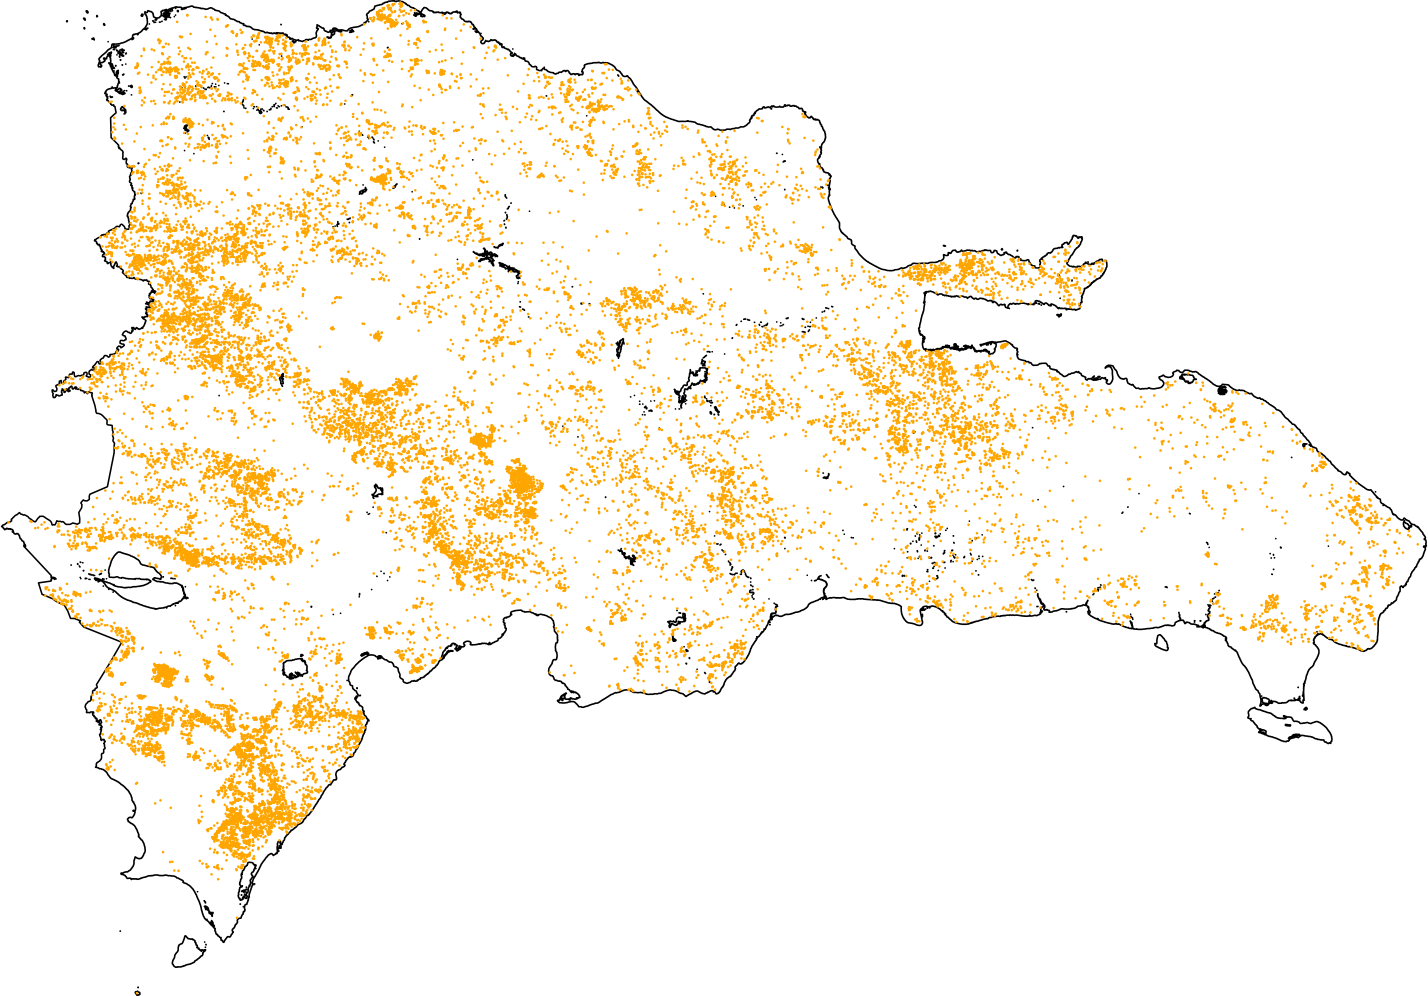
\includegraphics{img/data-download-preparation-eda/fires-m6-v1-sel2-2} \end{center}

\hypertarget{hotspotfire-layers-m6-and-v1-for-the-annual-analytical-approach}{%
\subsection{Hotspot/fire layers (M6 and V1) for the annual analytical
approach}\label{hotspotfire-layers-m6-and-v1-for-the-annual-analytical-approach}}

The hotspot/fire/thermal anomalies layers (M6 and V1) were created using
the script
\texttt{R/original-script-used-to-create-the-hotspot-fire-layers-M6-and-V1-for-annual-approach.R}.
This script was initially fed from a layer where thermal anomalies and
spontaneous fires from chimneys and landfills were manually removed from
each dataset, which were called ``noise-free versions of MODIS and VIIRS
datasets,'' respectively. Afterwards, annual maps of fire points using
the date field of the datasets were generated. Then, from the annual
maps of large clearings, buffer zones were created around the patches at
a maximum distance of 2.5 km. Lastly, the corresponding annual subsets
of fire points were generated by selecting only those falling within the
patches and/or their buffer zones.

\begin{Shaded}
\begin{Highlighting}[]
\CommentTok{\# Patches of forest loss \textgreater{} 1 ha. Fires M6, year 2001, intersected by forest{-}loss patches \textgreater{}1ha + 2.5 km buffer}
\NormalTok{loss1ha\_firesm6\_2500\_year2001 }\OtherTok{\textless{}{-}} \FunctionTok{readRDS}\NormalTok{(}\StringTok{\textquotesingle{}out/forest\_loss\_1ha\_firesm6\_2500\_buffer\_year\_2001.RDS\textquotesingle{}}\NormalTok{)}
\NormalTok{cline }\SpecialCharTok{\%\textgreater{}\%}\NormalTok{ as\_Spatial }\SpecialCharTok{\%\textgreater{}\%}\NormalTok{ plot}
\FunctionTok{plot}\NormalTok{(}
  \FunctionTok{as\_Spatial}\NormalTok{(loss1ha\_firesm6\_2500\_year2001),}
  \AttributeTok{main =} \StringTok{"Thermal anomalies from M6 dataset intersected by forest{-}loss patches \textgreater{}1ha + 2.5 km buffer, year 2001"}\NormalTok{,}
  \AttributeTok{pch =} \DecValTok{1}\NormalTok{, }\AttributeTok{cex =} \FloatTok{0.1}\NormalTok{, }\AttributeTok{add =}\NormalTok{ T, }\AttributeTok{col =} \StringTok{\textquotesingle{}orange\textquotesingle{}}\NormalTok{)}
\end{Highlighting}
\end{Shaded}

\begin{center}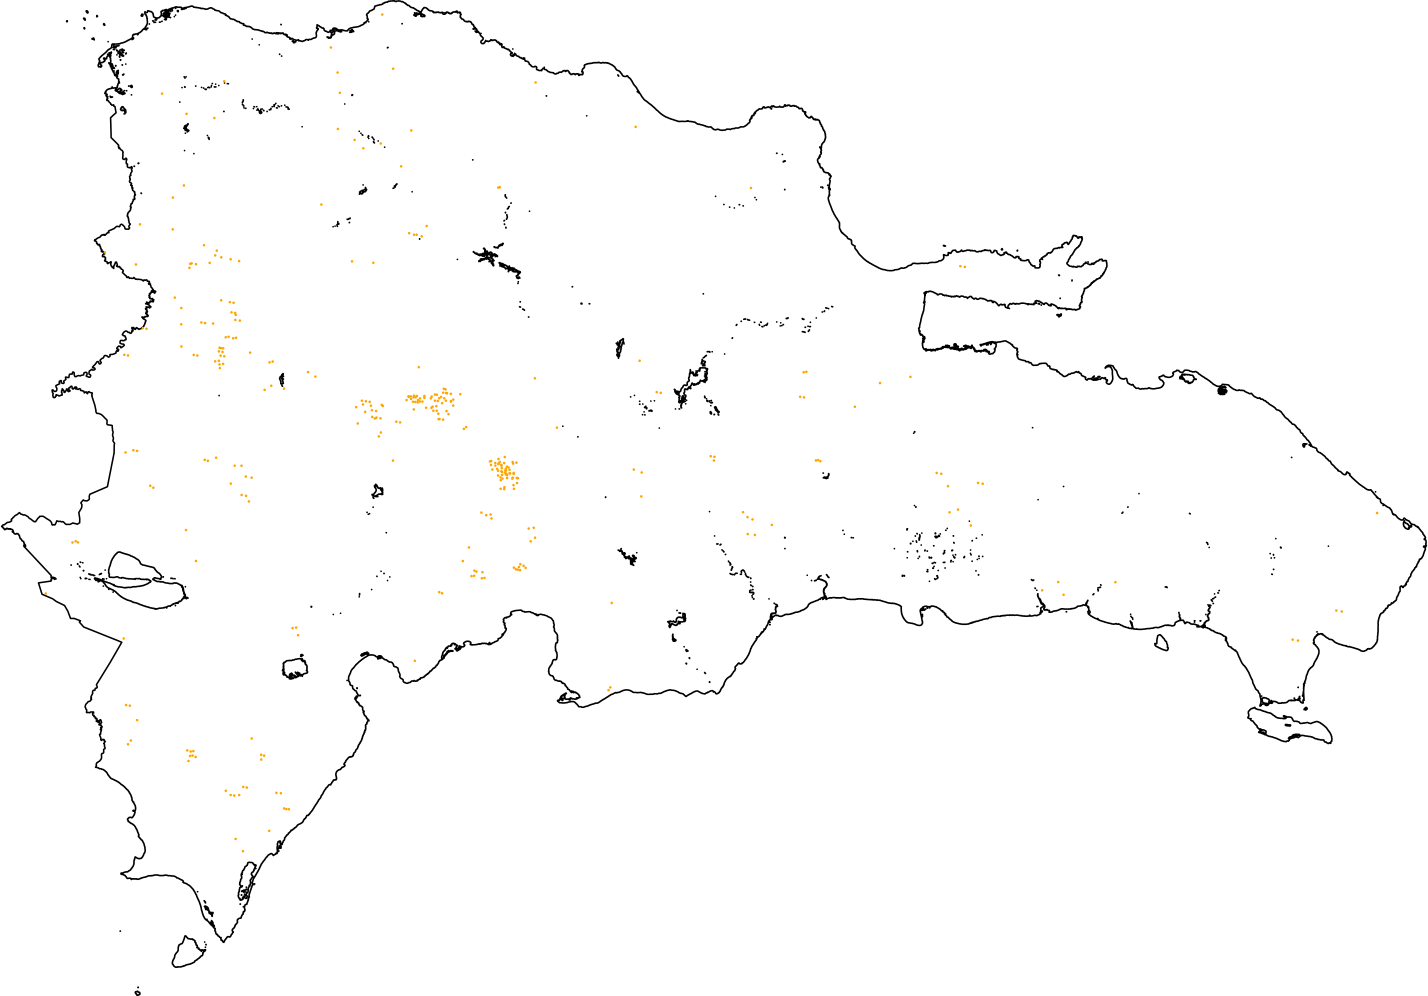
\includegraphics{img/data-download-preparation-eda/fires-m6-v1-sel-2500km-buffer-1} \end{center}

\begin{Shaded}
\begin{Highlighting}[]
\CommentTok{\# Patches of forest loss \textgreater{} 1 ha. Fires V1, year 2012, intersected by forest{-}loss patches \textgreater{}1ha + 2.5 km buffer}
\NormalTok{loss1ha\_firesv1\_2500\_year2012 }\OtherTok{\textless{}{-}} \FunctionTok{readRDS}\NormalTok{(}\StringTok{\textquotesingle{}out/forest\_loss\_1ha\_firesv1\_2500\_buffer\_year\_2012.RDS\textquotesingle{}}\NormalTok{)}
\NormalTok{cline }\SpecialCharTok{\%\textgreater{}\%}\NormalTok{ as\_Spatial }\SpecialCharTok{\%\textgreater{}\%}\NormalTok{ plot}
\FunctionTok{plot}\NormalTok{(}
  \FunctionTok{as\_Spatial}\NormalTok{(loss1ha\_firesv1\_2500\_year2012),}
  \AttributeTok{main =} \StringTok{"Thermal anomalies from V1 dataset intersected by forest{-}loss patches \textgreater{}1ha + 2.5 km buffer, year 2012"}\NormalTok{,}
  \AttributeTok{pch =} \DecValTok{1}\NormalTok{, }\AttributeTok{cex =} \FloatTok{0.1}\NormalTok{, }\AttributeTok{add =}\NormalTok{ T, }\AttributeTok{col =} \StringTok{\textquotesingle{}orange\textquotesingle{}}\NormalTok{)}
\end{Highlighting}
\end{Shaded}

\begin{center}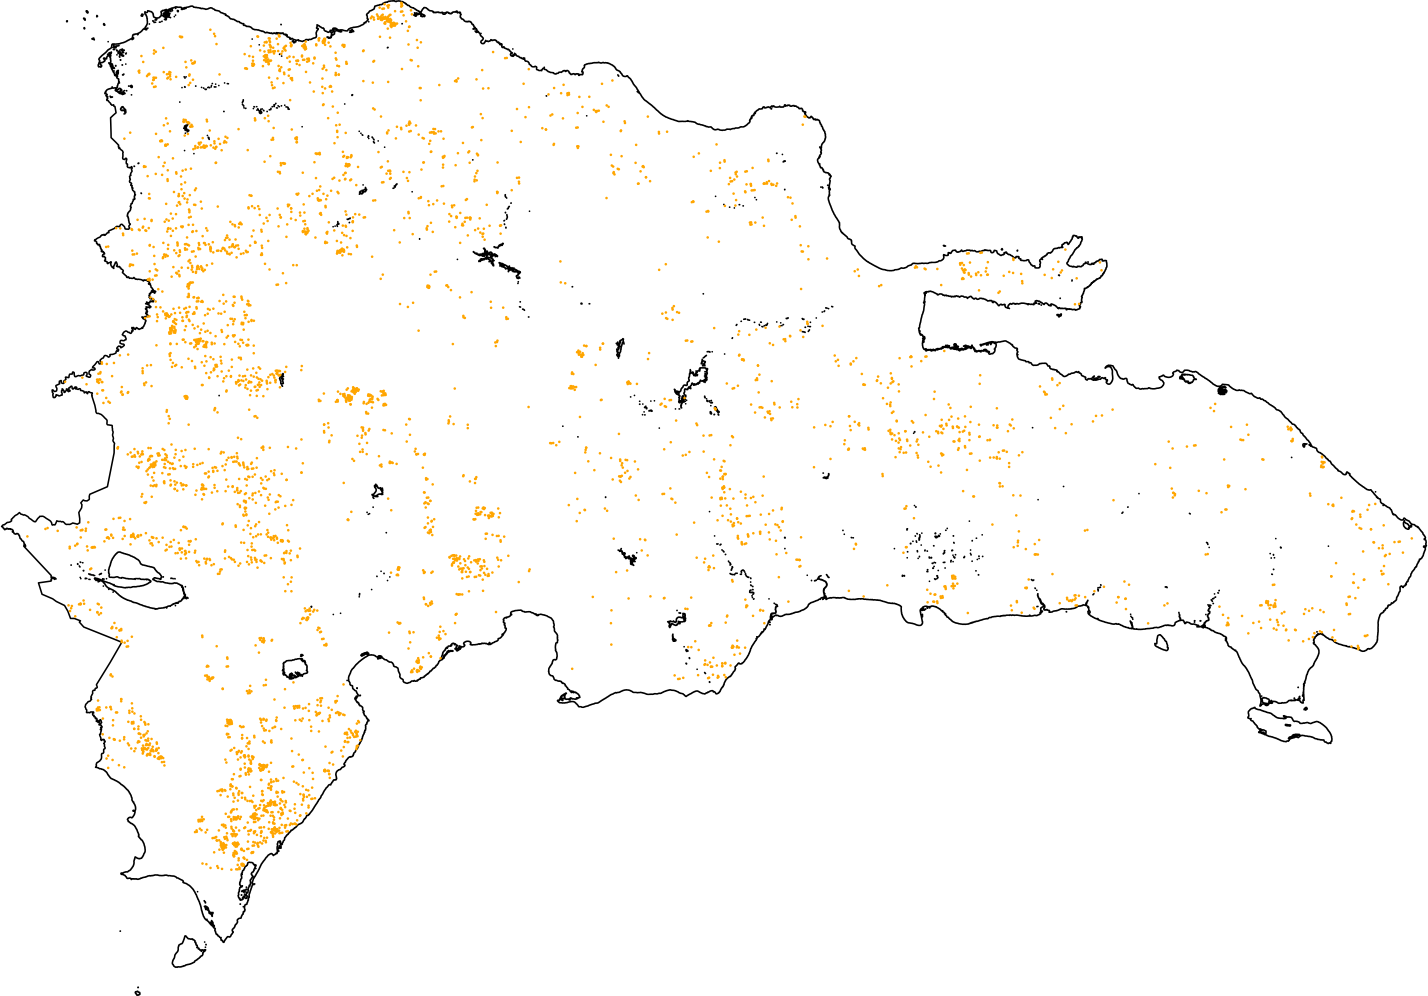
\includegraphics{img/data-download-preparation-eda/fires-m6-v1-sel-2500km-buffer-2} \end{center}

\hypertarget{grid-layers-for-modelling}{%
\section{Grid layers for modelling}\label{grid-layers-for-modelling}}

The models generated in this study are referred to zonal statistics
computed using different regular grids for long-term and annual
approaches

\hypertarget{long-term-approach-analysis-grid}{%
\subsection{Long-term approach analysis
grid}\label{long-term-approach-analysis-grid}}

The regular grid for the long-term approach, loaded in the following
code chunk, was generated using the script
\texttt{R/original-script-used-to-create-the-grid-long-term-approach.R}.
For practical reasons, the grid is simply loaded using the
\texttt{readRDS} function.

\begin{Shaded}
\begin{Highlighting}[]
\NormalTok{grd }\OtherTok{\textless{}{-}} \FunctionTok{readRDS}\NormalTok{(}\StringTok{\textquotesingle{}out/grd\_plain\_only\_area\_known\_in\_R\_as\_grd.RDS\textquotesingle{}}\NormalTok{)}
\NormalTok{grd}
\DocumentationTok{\#\# Simple feature collection with 482 features and 3 fields}
\DocumentationTok{\#\# Geometry type: POLYGON}
\DocumentationTok{\#\# Dimension:     XY}
\DocumentationTok{\#\# Bounding box:  xmin: 187612.2 ymin: 1955288 xmax: 569084.5 ymax: 2209654}
\DocumentationTok{\#\# Projected CRS: WGS 84 / UTM zone 19N}
\DocumentationTok{\#\# First 10 features:}
\DocumentationTok{\#\#    ENLACE  AREASQM AREASQM\_PCT                       geometry}
\DocumentationTok{\#\# 1       1 47325583    47.32558 POLYGON ((192985 2057655, 1...}
\DocumentationTok{\#\# 2       2 99988965    99.98896 POLYGON ((198357.9 2048349,...}
\DocumentationTok{\#\# 3       3 99522753    99.52275 POLYGON ((203730.7 2039043,...}
\DocumentationTok{\#\# 4       4 65772385    65.77239 POLYGON ((203730.7 2057655,...}
\DocumentationTok{\#\# 5       5 49396881    49.39688 POLYGON ((203730.7 2094879,...}
\DocumentationTok{\#\# 6       6 62199862    62.19986 POLYGON ((209103.6 2011125,...}
\DocumentationTok{\#\# 7       7 84439177    84.43918 POLYGON ((209103.6 2029737,...}
\DocumentationTok{\#\# 8       8 92450749    92.45075 POLYGON ((209103.6 2048349,...}
\DocumentationTok{\#\# 9       9 98900253    98.90025 POLYGON ((214476.4 2001819,...}
\DocumentationTok{\#\# 10     10 68962809    68.96281 POLYGON ((214476.4 2020431,...}
\NormalTok{cline }\SpecialCharTok{\%\textgreater{}\%}\NormalTok{ as\_Spatial }\SpecialCharTok{\%\textgreater{}\%}\NormalTok{ plot}
\NormalTok{grd }\SpecialCharTok{\%\textgreater{}\%}\NormalTok{ as\_Spatial }\SpecialCharTok{\%\textgreater{}\%} \FunctionTok{plot}\NormalTok{(}\AttributeTok{add=}\NormalTok{T)}
\end{Highlighting}
\end{Shaded}

\begin{center}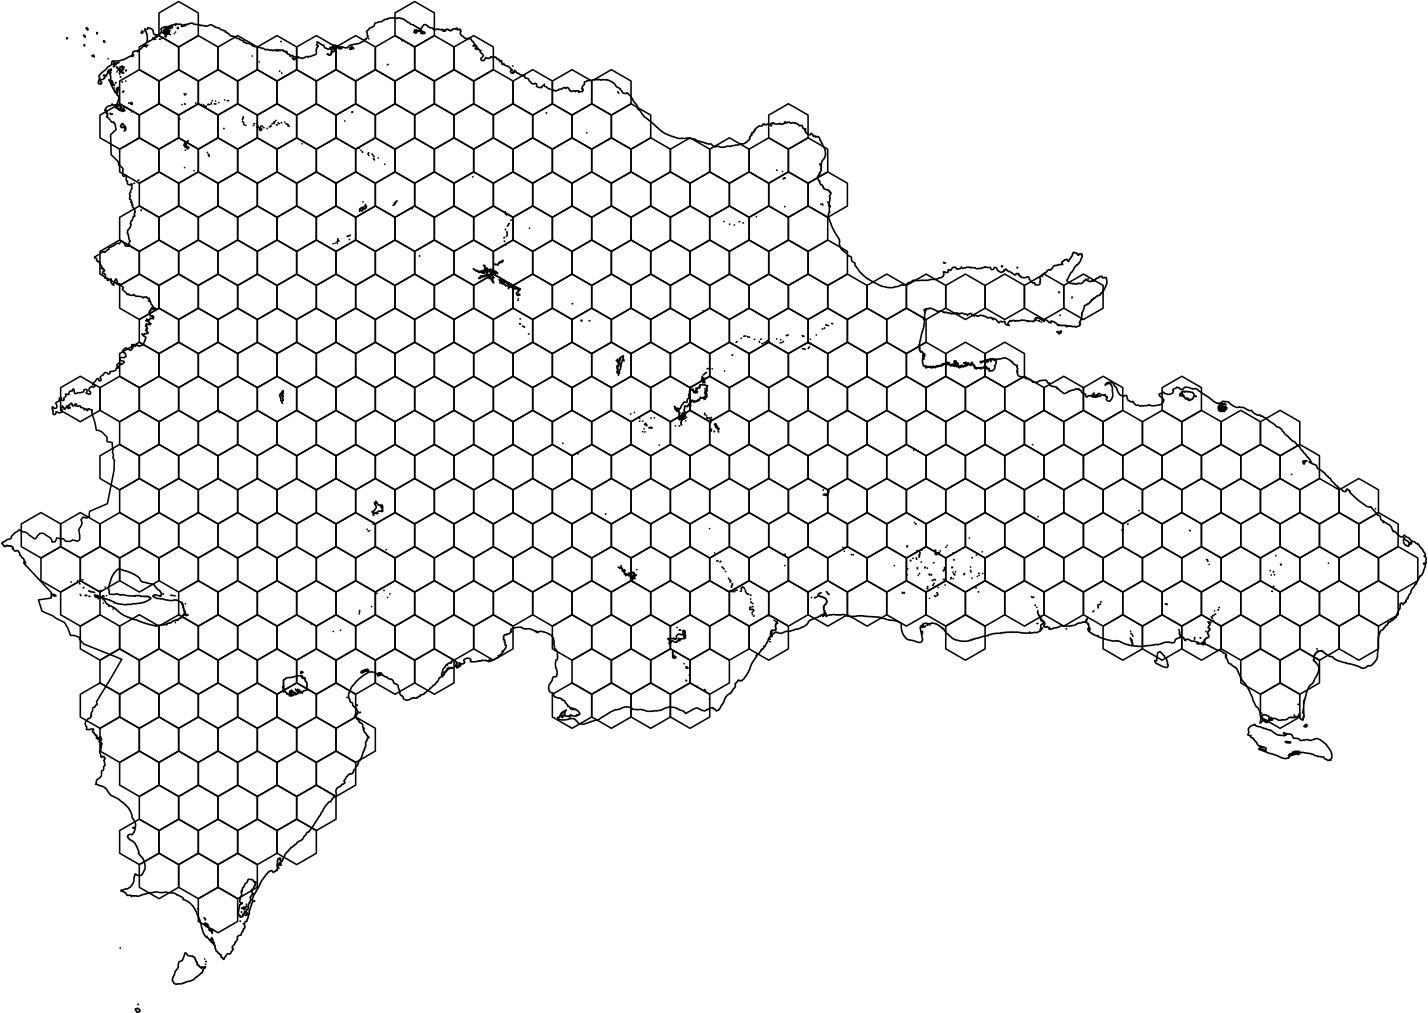
\includegraphics{img/data-download-preparation-eda/regular-grid-1} \end{center}

\hypertarget{annual-approach-analysis-grid}{%
\subsection{Annual approach analysis
grid}\label{annual-approach-analysis-grid}}

The regular grid for the long-term approach, loaded in the following
code chunk, was generated using the script
\texttt{R/original-script-used-to-create-the-grid-annual-approach.R}.
For practical reasons, the grid is simply loaded using the
\texttt{readRDS} function.

\begin{Shaded}
\begin{Highlighting}[]
\NormalTok{hexsf }\OtherTok{\textless{}{-}} \FunctionTok{readRDS}\NormalTok{(}\StringTok{\textquotesingle{}out/honeycomb\_grid\_sf.RDS\textquotesingle{}}\NormalTok{)}
\NormalTok{hexsf}
\DocumentationTok{\#\# Simple feature collection with 253 features and 6 fields}
\DocumentationTok{\#\# Geometry type: POLYGON}
\DocumentationTok{\#\# Dimension:     XY}
\DocumentationTok{\#\# Bounding box:  xmin: 182239.3 ymin: 1953895 xmax: 572239.3 ymax: 2205042}
\DocumentationTok{\#\# Projected CRS: WGS 84 / UTM zone 19N}
\DocumentationTok{\#\# First 10 features:}
\DocumentationTok{\#\#    ENLACE a0\_square\_meters   AREASQM AREASQM\_PCT     xutm    yutm}
\DocumentationTok{\#\# 1       1        194855716  81359197    41.75356 189739.3 2053488}
\DocumentationTok{\#\# 2       2        194855716  89453896    45.90776 197239.3 2040497}
\DocumentationTok{\#\# 3       3        194855716 192920585    99.00689 204739.3 2053488}
\DocumentationTok{\#\# 4       4        194855716 168639558    86.54586 212239.3 2014517}
\DocumentationTok{\#\# 5       5        194855716 166723114    85.56234 212239.3 2040497}
\DocumentationTok{\#\# 6       6        194855716 182554622    93.68708 212239.3 2066478}
\DocumentationTok{\#\# 7       7        194855716 135315105    69.44374 212239.3 2092459}
\DocumentationTok{\#\# 8       8        194855716  85442381    43.84905 212239.3 2170401}
\DocumentationTok{\#\# 9       9        194855716 105127666    53.95154 219739.3 1975545}
\DocumentationTok{\#\# 10     10        194855716 194855716   100.00000 219739.3 2001526}
\DocumentationTok{\#\#                          geometry}
\DocumentationTok{\#\# 1  POLYGON ((189739.3 2044827,...}
\DocumentationTok{\#\# 2  POLYGON ((197239.3 2031837,...}
\DocumentationTok{\#\# 3  POLYGON ((204739.3 2044827,...}
\DocumentationTok{\#\# 4  POLYGON ((212239.3 2005856,...}
\DocumentationTok{\#\# 5  POLYGON ((212239.3 2031837,...}
\DocumentationTok{\#\# 6  POLYGON ((212239.3 2057818,...}
\DocumentationTok{\#\# 7  POLYGON ((212239.3 2083799,...}
\DocumentationTok{\#\# 8  POLYGON ((212239.3 2161741,...}
\DocumentationTok{\#\# 9  POLYGON ((219739.3 1966885,...}
\DocumentationTok{\#\# 10 POLYGON ((219739.3 1992866,...}
\NormalTok{cline }\SpecialCharTok{\%\textgreater{}\%}\NormalTok{ as\_Spatial }\SpecialCharTok{\%\textgreater{}\%}\NormalTok{ plot}
\NormalTok{hexsf }\SpecialCharTok{\%\textgreater{}\%}\NormalTok{ as\_Spatial }\SpecialCharTok{\%\textgreater{}\%} \FunctionTok{plot}\NormalTok{(}\AttributeTok{add=}\NormalTok{T)}
\end{Highlighting}
\end{Shaded}

\begin{center}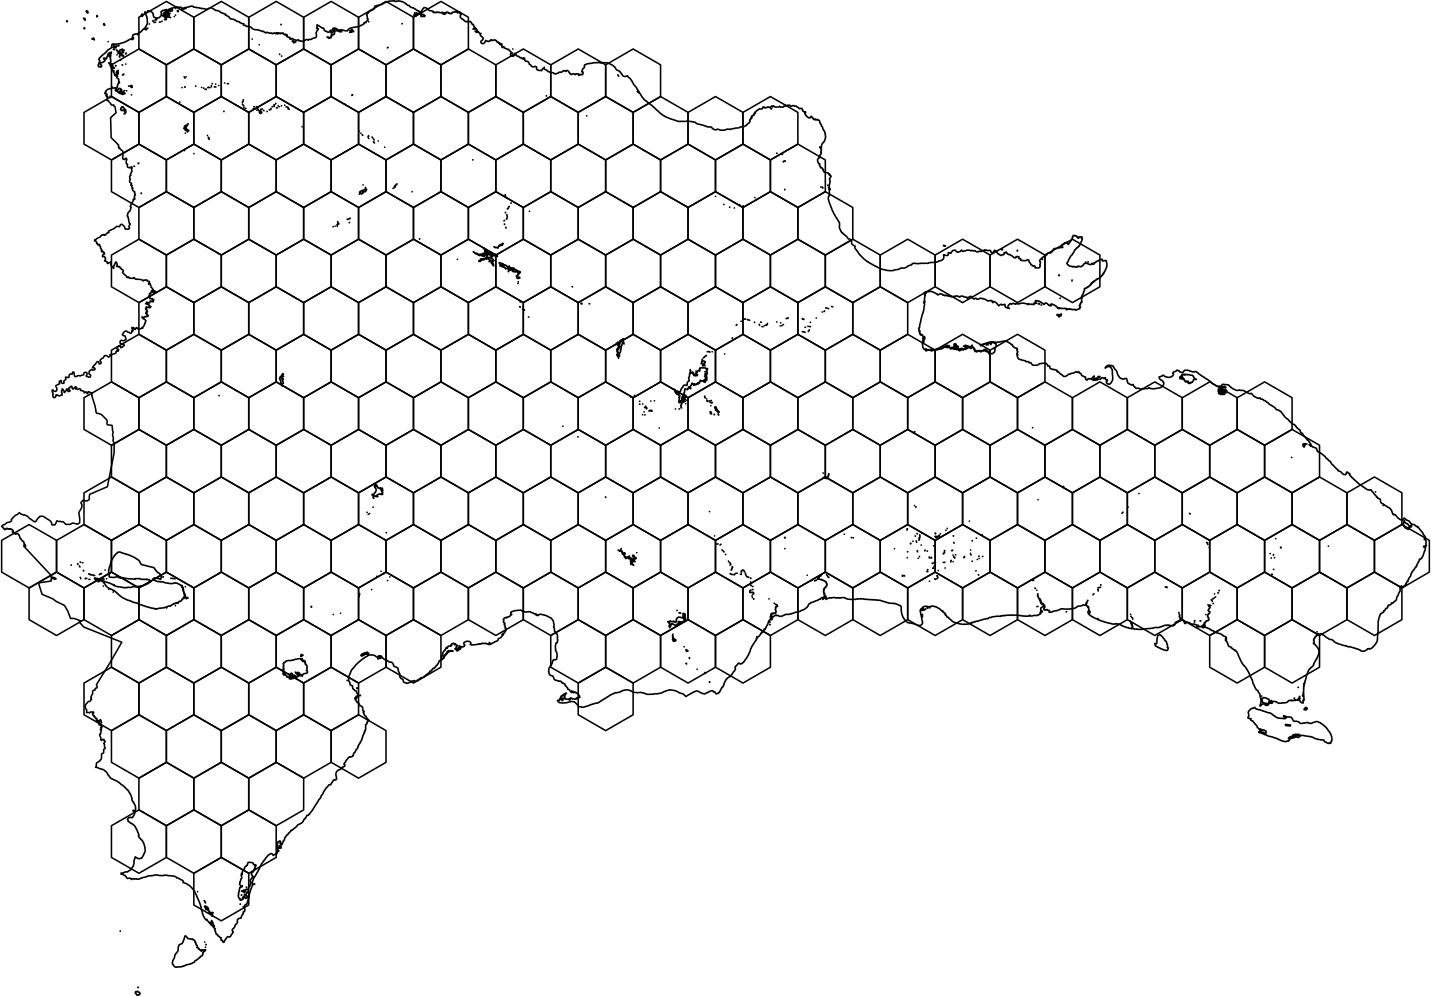
\includegraphics{img/data-download-preparation-eda/hex-grid-annual-approach-1} \end{center}

\hypertarget{zonal-statistic-computations}{%
\section{Zonal statistic
computations}\label{zonal-statistic-computations}}

Many zonal statistics were performed using different zone layers. These
computations may assit policy information and decision-making processes.
These tasks were performed in semi-automatic mode using R scripts. Since
such scripts produced intermediate results, they are not essential to
reproduce this RMarkdown. However, if one or more scripts should be run,
it would be sufficient to open and run them in one go.

\hypertarget{zonal-statistics-by-provinces}{%
\subsection{Zonal statistics by
provinces}\label{zonal-statistics-by-provinces}}

The script used to compute zonal statistics is stored in
\texttt{R/original-script-used-to-compute-zonal-statistics-provinces.R}.
For practical reasons and for future use (e.g.~in the EDA section), the
results of the script were saved to an RDS file located at
\texttt{out/prov\_zonal\_statistics.RDS}.

\hypertarget{zonal-statistics-by-municipalities}{%
\subsection{Zonal statistics by
municipalities}\label{zonal-statistics-by-municipalities}}

The script used to compute zonal statistics is stored in
\texttt{R/original-script-used-to-compute-zonal-statistics-municipalities.R}.
For practical reasons and for future use (e.g.~in the EDA section), the
results of the script were saved to an RDS file located at
\texttt{out/mun\_zonal\_statistics.RDS}.

\hypertarget{zonal-statistics-by-protected-areas}{%
\subsection{Zonal statistics by protected
areas}\label{zonal-statistics-by-protected-areas}}

The script used to compute zonal statistics is stored in
\texttt{R/original-script-used-to-compute-zonal-statistics-protected-areas.R}.
It is worth mentioning that protected areas with less than 3 sq. km and
less than 30\% within cutline, were excluded in the script. For
practical reasons and for future use (e.g.~in the EDA section), the
results of the script were saved to an RDS file located at
\texttt{out/pa\_zonal\_statistics.RDS}.

\hypertarget{zonal-statistics-by-grid-used-in-the-long-term-analytical-approach}{%
\subsection{Zonal statistics by grid used in the long-term analytical
approach}\label{zonal-statistics-by-grid-used-in-the-long-term-analytical-approach}}

The script used to compute zonal statistics is stored in
\texttt{R/original-script-used-to-compute-zonal-statistics-grid-long-term-approach.R}.
For practical reasons and for future use (e.g.~in the EDA section), the
results of the script were saved to an RDS file located at
\texttt{out/grd\_zonal\_statistics.RDS}.

\hypertarget{zonal-statistics-by-grid-used-in-the-annual-analytical-approach}{%
\subsection{Zonal statistics by grid used in the annual analytical
approach}\label{zonal-statistics-by-grid-used-in-the-annual-analytical-approach}}

The script used to compute zonal statistics is stored in
\texttt{R/original-script-used-to-compute-zonal-statistics-grid-annual-approach.R}.
For practical reasons and for future use (e.g.~in the EDA section), the
results of the script were saved to an RDS file located at
\texttt{out/hex\_zonal\_statistics.RDS}.

\hypertarget{exploratory-data-analisys-eda}{%
\section{Exploratory data analisys
(EDA)}\label{exploratory-data-analisys-eda}}

\hypertarget{at-national-level-no-zonal-analysis}{%
\subsection{At National level, no zonal
analysis}\label{at-national-level-no-zonal-analysis}}

\hypertarget{tree-canopy-cover-of-year-2000-classes-area-in-km2-and-percentages}{%
\subsubsection{Tree canopy cover of year 2000 classes: area in km\^{}2
and
percentages}\label{tree-canopy-cover-of-year-2000-classes-area-in-km2-and-percentages}}

\begin{Shaded}
\begin{Highlighting}[]
\NormalTok{tct }\OtherTok{\textless{}{-}} \FunctionTok{table}\NormalTok{(tc[])}
\NormalTok{tcsum }\OtherTok{\textless{}{-}}\NormalTok{ tct }\SpecialCharTok{\%\textgreater{}\%}\NormalTok{ as.data.frame }\SpecialCharTok{\%\textgreater{}\%}
  \FunctionTok{mutate}\NormalTok{(}
    \AttributeTok{treecover =} \FunctionTok{as.numeric}\NormalTok{(}\FunctionTok{as.character}\NormalTok{(Var1)),}
    \StringTok{\textasciigrave{}}\AttributeTok{sq. km}\StringTok{\textasciigrave{}} \OtherTok{=}\NormalTok{ Freq}\SpecialCharTok{*}\FunctionTok{prod}\NormalTok{(}\FunctionTok{res}\NormalTok{(tc))}\SpecialCharTok{/}\DecValTok{1000000}\NormalTok{,}
    \AttributeTok{pct =}\NormalTok{ Freq}\SpecialCharTok{/}\FunctionTok{sum}\NormalTok{(Freq)}\SpecialCharTok{*}\DecValTok{100}\NormalTok{) }\SpecialCharTok{\%\textgreater{}\%}
\NormalTok{  dplyr}\SpecialCharTok{::}\FunctionTok{select}\NormalTok{(}\SpecialCharTok{{-}}\NormalTok{Var1, }\SpecialCharTok{{-}}\NormalTok{Freq) }\SpecialCharTok{\%\textgreater{}\%} 
  \FunctionTok{mutate}\NormalTok{(}\StringTok{\textasciigrave{}}\AttributeTok{Tree canopy cover for year 2000}\StringTok{\textasciigrave{}} \OtherTok{=} \FunctionTok{case\_when}\NormalTok{(}
\NormalTok{    treecover }\SpecialCharTok{\textless{}=} \DecValTok{25} \SpecialCharTok{\textasciitilde{}} \StringTok{\textquotesingle{}0{-}25\%\textquotesingle{}}\NormalTok{,}
\NormalTok{    treecover }\SpecialCharTok{\textgreater{}=} \DecValTok{26} \SpecialCharTok{\&}\NormalTok{ treecover }\SpecialCharTok{\textless{}=} \DecValTok{50} \SpecialCharTok{\textasciitilde{}} \StringTok{\textquotesingle{}26{-}50\%\textquotesingle{}}\NormalTok{,}
\NormalTok{    treecover }\SpecialCharTok{\textgreater{}=} \DecValTok{51} \SpecialCharTok{\&}\NormalTok{ treecover }\SpecialCharTok{\textless{}=} \DecValTok{75} \SpecialCharTok{\textasciitilde{}} \StringTok{\textquotesingle{}51{-}75\%\textquotesingle{}}\NormalTok{,}
\NormalTok{    treecover }\SpecialCharTok{\textgreater{}=} \DecValTok{76} \SpecialCharTok{\textasciitilde{}} \StringTok{\textquotesingle{}76{-}100\%\textquotesingle{}}
\NormalTok{  )) }\SpecialCharTok{\%\textgreater{}\%}
  \FunctionTok{group\_by}\NormalTok{(}\StringTok{\textasciigrave{}}\AttributeTok{Tree canopy cover for year 2000}\StringTok{\textasciigrave{}}\NormalTok{) }\SpecialCharTok{\%\textgreater{}\%}
  \FunctionTok{summarise\_each}\NormalTok{(}\FunctionTok{funs}\NormalTok{(}\FunctionTok{sum}\NormalTok{(.)), (}\StringTok{\textasciigrave{}}\AttributeTok{sq. km}\StringTok{\textasciigrave{}}\SpecialCharTok{:}\NormalTok{pct))}
\NormalTok{tcsum}
\DocumentationTok{\#\# \# A tibble: 4 x 3}
\DocumentationTok{\#\#   \textasciigrave{}Tree canopy cover for year 2000\textasciigrave{} \textasciigrave{}sq. km\textasciigrave{}   pct}
\DocumentationTok{\#\#   \textless{}chr\textgreater{}                                \textless{}dbl\textgreater{} \textless{}dbl\textgreater{}}
\DocumentationTok{\#\# 1 0{-}25\%                               21455. 44.8 }
\DocumentationTok{\#\# 2 26{-}50\%                               4076.  8.50}
\DocumentationTok{\#\# 3 51{-}75\%                               4631.  9.66}
\DocumentationTok{\#\# 4 76{-}100\%                             17762. 37.1}
\NormalTok{tcsum }\SpecialCharTok{\%\textgreater{}\%}
  \FunctionTok{ggplot}\NormalTok{() }\SpecialCharTok{+} \FunctionTok{aes}\NormalTok{(}\AttributeTok{x =} \StringTok{\textasciigrave{}}\AttributeTok{Tree canopy cover for year 2000}\StringTok{\textasciigrave{}}\NormalTok{, }\AttributeTok{y =} \StringTok{\textasciigrave{}}\AttributeTok{sq. km}\StringTok{\textasciigrave{}}\NormalTok{) }\SpecialCharTok{+}
  \FunctionTok{theme\_bw}\NormalTok{() }\SpecialCharTok{+} \FunctionTok{geom\_col}\NormalTok{(}\AttributeTok{width =} \FloatTok{0.45}\NormalTok{) }\SpecialCharTok{+} \FunctionTok{theme}\NormalTok{(}\AttributeTok{text =} \FunctionTok{element\_text}\NormalTok{(}\AttributeTok{size =} \DecValTok{16}\NormalTok{))}
\end{Highlighting}
\end{Shaded}

\begin{center}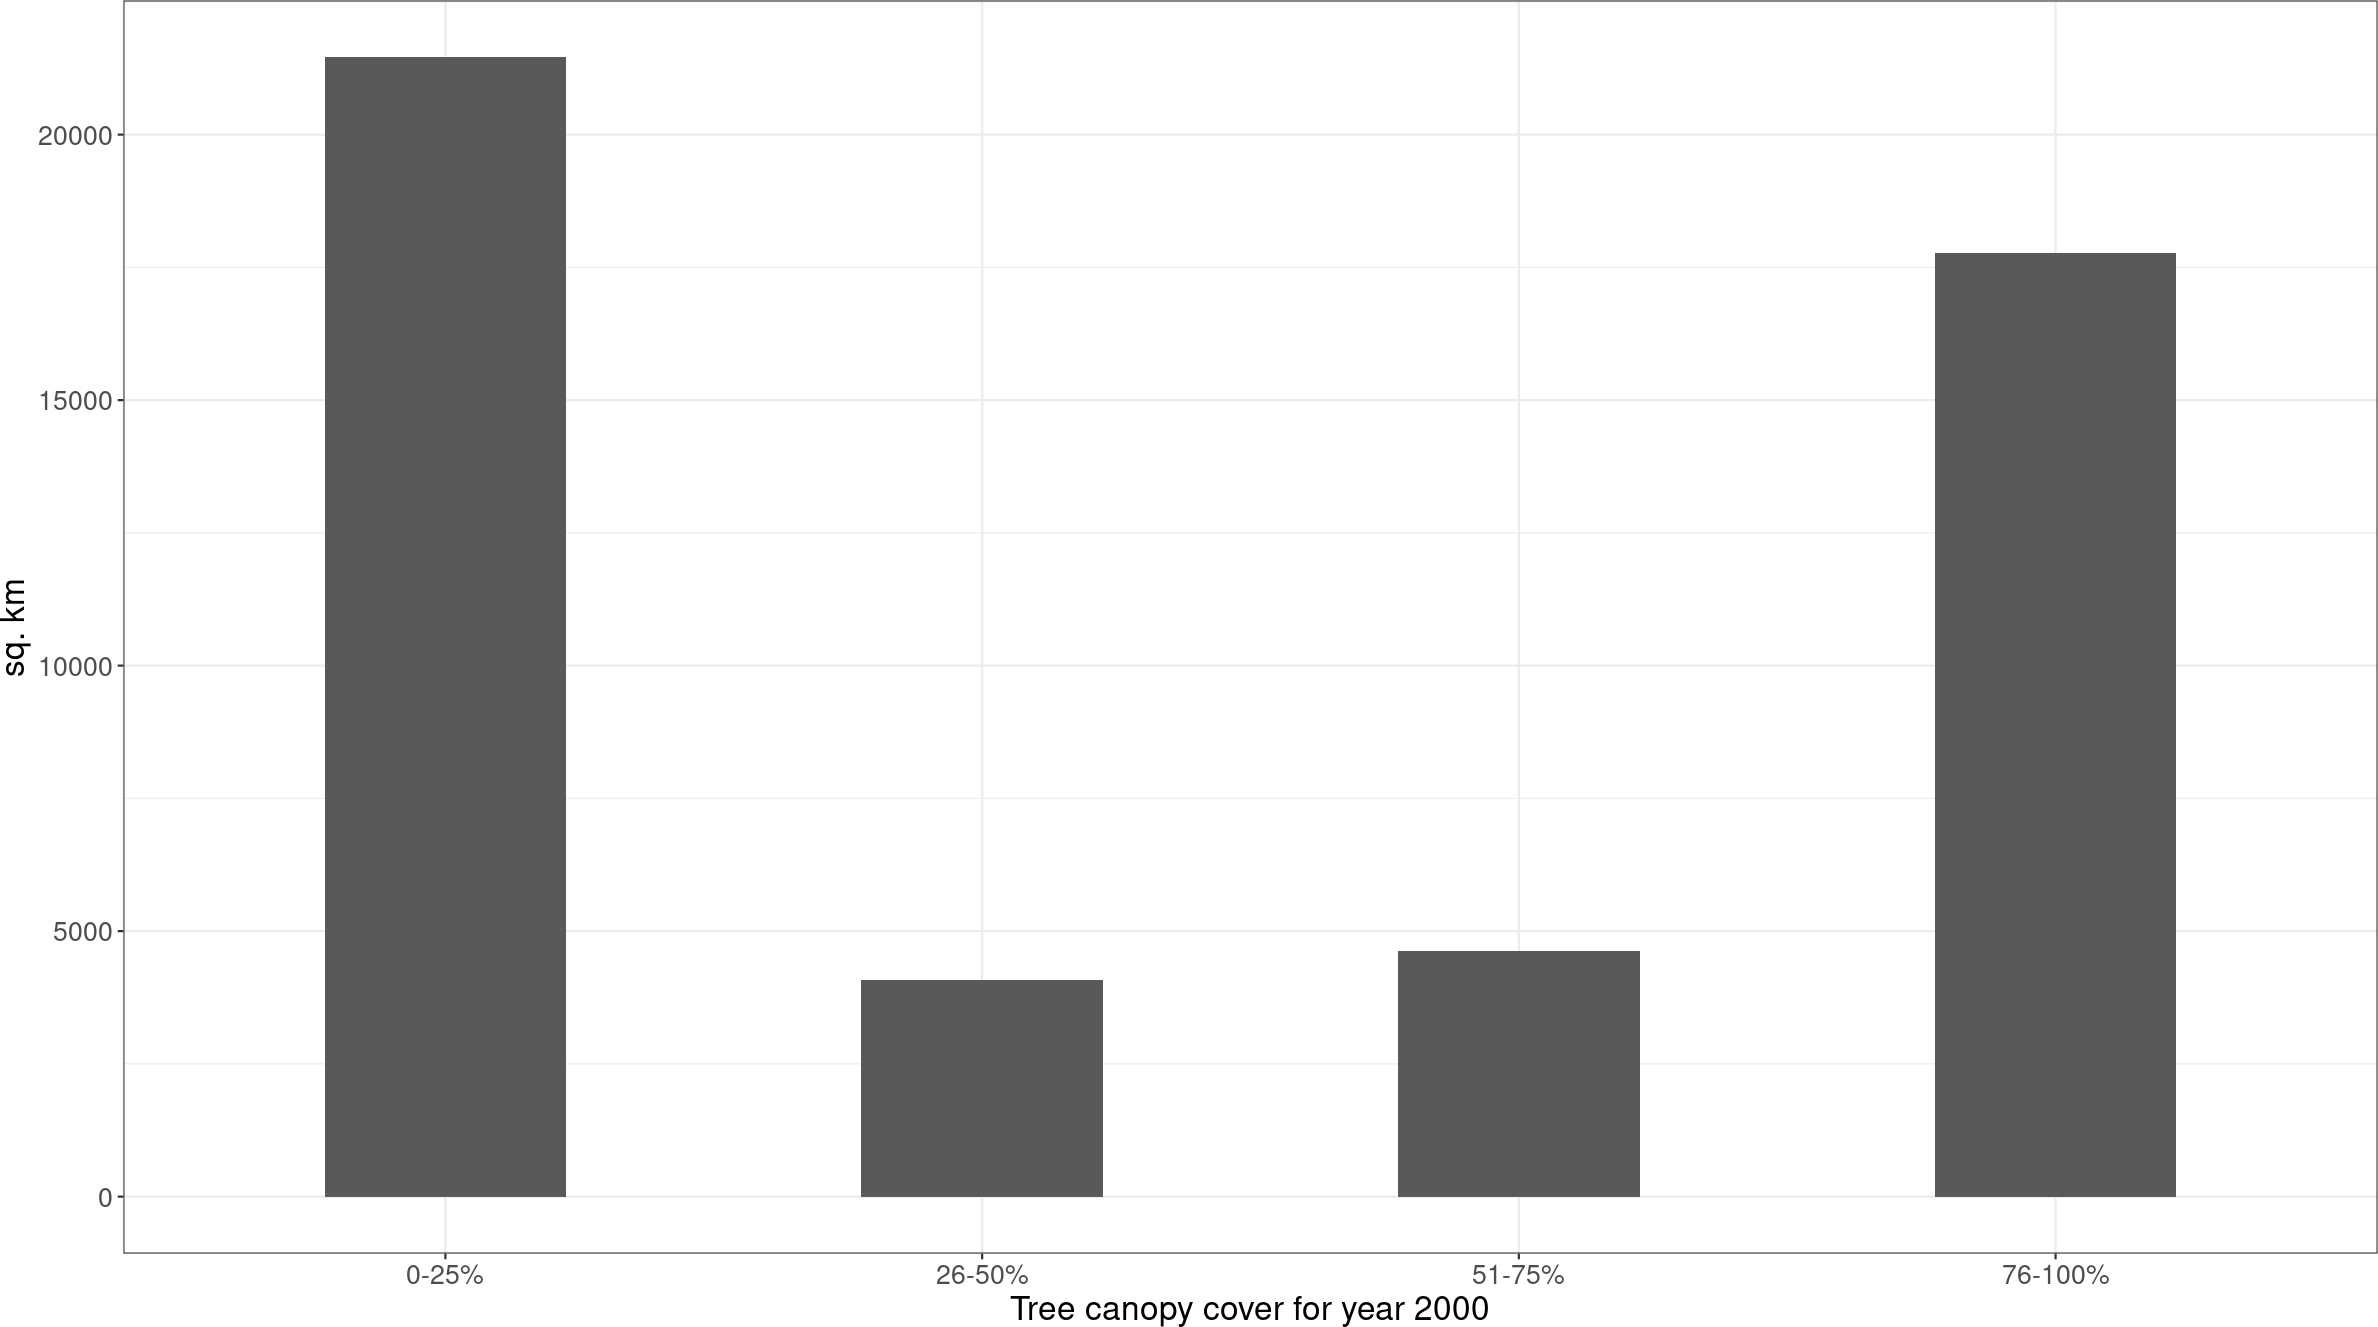
\includegraphics[width=0.5\linewidth]{img/data-download-preparation-eda/tree-canopy-cover-2000-nationwide-by-year-1} \end{center}

\hypertarget{year-of-gross-forest-cover-loss-2001-2018-area-in-km2-and-percentages}{%
\subsubsection{Year of gross forest cover loss (2001-2018): area in
km\^{}2 and
percentages}\label{year-of-gross-forest-cover-loss-2001-2018-area-in-km2-and-percentages}}

\begin{itemize}
\tightlist
\item
  By year
\end{itemize}

\begin{Shaded}
\begin{Highlighting}[]
\NormalTok{lyt }\OtherTok{\textless{}{-}} \FunctionTok{table}\NormalTok{(ly[])}
\NormalTok{lysum }\OtherTok{\textless{}{-}}\NormalTok{ lyt }\SpecialCharTok{\%\textgreater{}\%}\NormalTok{ as.data.frame }\SpecialCharTok{\%\textgreater{}\%}
  \FunctionTok{mutate}\NormalTok{(}
    \StringTok{\textasciigrave{}}\AttributeTok{Year of gross forest cover loss}\StringTok{\textasciigrave{}} \OtherTok{=} \FunctionTok{as.numeric}\NormalTok{(}\FunctionTok{as.character}\NormalTok{(Var1)) }\SpecialCharTok{+} \DecValTok{2000}\NormalTok{,}
    \StringTok{\textasciigrave{}}\AttributeTok{sq. km}\StringTok{\textasciigrave{}} \OtherTok{=}\NormalTok{ Freq}\SpecialCharTok{*}\FunctionTok{prod}\NormalTok{(}\FunctionTok{res}\NormalTok{(ly))}\SpecialCharTok{/}\DecValTok{1000000}\NormalTok{,}
    \AttributeTok{pct =}\NormalTok{ Freq}\SpecialCharTok{/}\FunctionTok{sum}\NormalTok{(Freq)}\SpecialCharTok{*}\DecValTok{100}\NormalTok{) }\SpecialCharTok{\%\textgreater{}\%}
\NormalTok{  dplyr}\SpecialCharTok{::}\FunctionTok{select}\NormalTok{(}\SpecialCharTok{{-}}\NormalTok{Var1, }\SpecialCharTok{{-}}\NormalTok{Freq)}
\NormalTok{lysum}
\DocumentationTok{\#\#    Year of gross forest cover loss     sq. km        pct}
\DocumentationTok{\#\# 1                             2000 44608.0329 93.0816470}
\DocumentationTok{\#\# 2                             2001   117.4182  0.2450114}
\DocumentationTok{\#\# 3                             2002   109.6281  0.2287562}
\DocumentationTok{\#\# 4                             2003   112.7959  0.2353664}
\DocumentationTok{\#\# 5                             2004   203.3267  0.4242729}
\DocumentationTok{\#\# 6                             2005   259.6146  0.5417266}
\DocumentationTok{\#\# 7                             2006   144.4874  0.3014955}
\DocumentationTok{\#\# 8                             2007   169.8247  0.3543659}
\DocumentationTok{\#\# 9                             2008   225.6897  0.4709369}
\DocumentationTok{\#\# 10                            2009   147.2277  0.3072137}
\DocumentationTok{\#\# 11                            2010   146.8974  0.3065245}
\DocumentationTok{\#\# 12                            2011   136.6796  0.2852035}
\DocumentationTok{\#\# 13                            2012   193.7474  0.4042844}
\DocumentationTok{\#\# 14                            2013   178.2085  0.3718599}
\DocumentationTok{\#\# 15                            2014   179.2863  0.3741089}
\DocumentationTok{\#\# 16                            2015   186.6761  0.3895290}
\DocumentationTok{\#\# 17                            2016   291.0449  0.6073108}
\DocumentationTok{\#\# 18                            2017   330.4609  0.6895584}
\DocumentationTok{\#\# 19                            2018   182.5063  0.3808280}
\NormalTok{lysum }\SpecialCharTok{\%\textgreater{}\%}\NormalTok{ dplyr}\SpecialCharTok{::}\FunctionTok{filter}\NormalTok{(}\StringTok{\textasciigrave{}}\AttributeTok{Year of gross forest cover loss}\StringTok{\textasciigrave{}}\SpecialCharTok{\textgreater{}}\DecValTok{2000}\NormalTok{) }\SpecialCharTok{\%\textgreater{}\%} 
  \FunctionTok{ggplot}\NormalTok{() }\SpecialCharTok{+} \FunctionTok{aes}\NormalTok{(}\AttributeTok{x =} \StringTok{\textasciigrave{}}\AttributeTok{Year of gross forest cover loss}\StringTok{\textasciigrave{}}\NormalTok{, }\AttributeTok{y =} \StringTok{\textasciigrave{}}\AttributeTok{sq. km}\StringTok{\textasciigrave{}}\NormalTok{) }\SpecialCharTok{+}
  \FunctionTok{theme\_bw}\NormalTok{() }\SpecialCharTok{+} \FunctionTok{geom\_col}\NormalTok{(}\AttributeTok{width =} \FloatTok{0.45}\NormalTok{) }\SpecialCharTok{+}
  \FunctionTok{scale\_x\_continuous}\NormalTok{(}\AttributeTok{breaks =}\NormalTok{ lysum}\SpecialCharTok{$}\StringTok{\textasciigrave{}}\AttributeTok{Year of gross forest cover loss}\StringTok{\textasciigrave{}}\NormalTok{) }\SpecialCharTok{+}
  \FunctionTok{theme}\NormalTok{(}\AttributeTok{axis.text.x =} \FunctionTok{element\_text}\NormalTok{(}\AttributeTok{angle =} \DecValTok{90}\NormalTok{, }\AttributeTok{vjust =} \FloatTok{0.5}\NormalTok{), }\AttributeTok{text =} \FunctionTok{element\_text}\NormalTok{(}\AttributeTok{size =} \DecValTok{16}\NormalTok{))}
\end{Highlighting}
\end{Shaded}

\begin{center}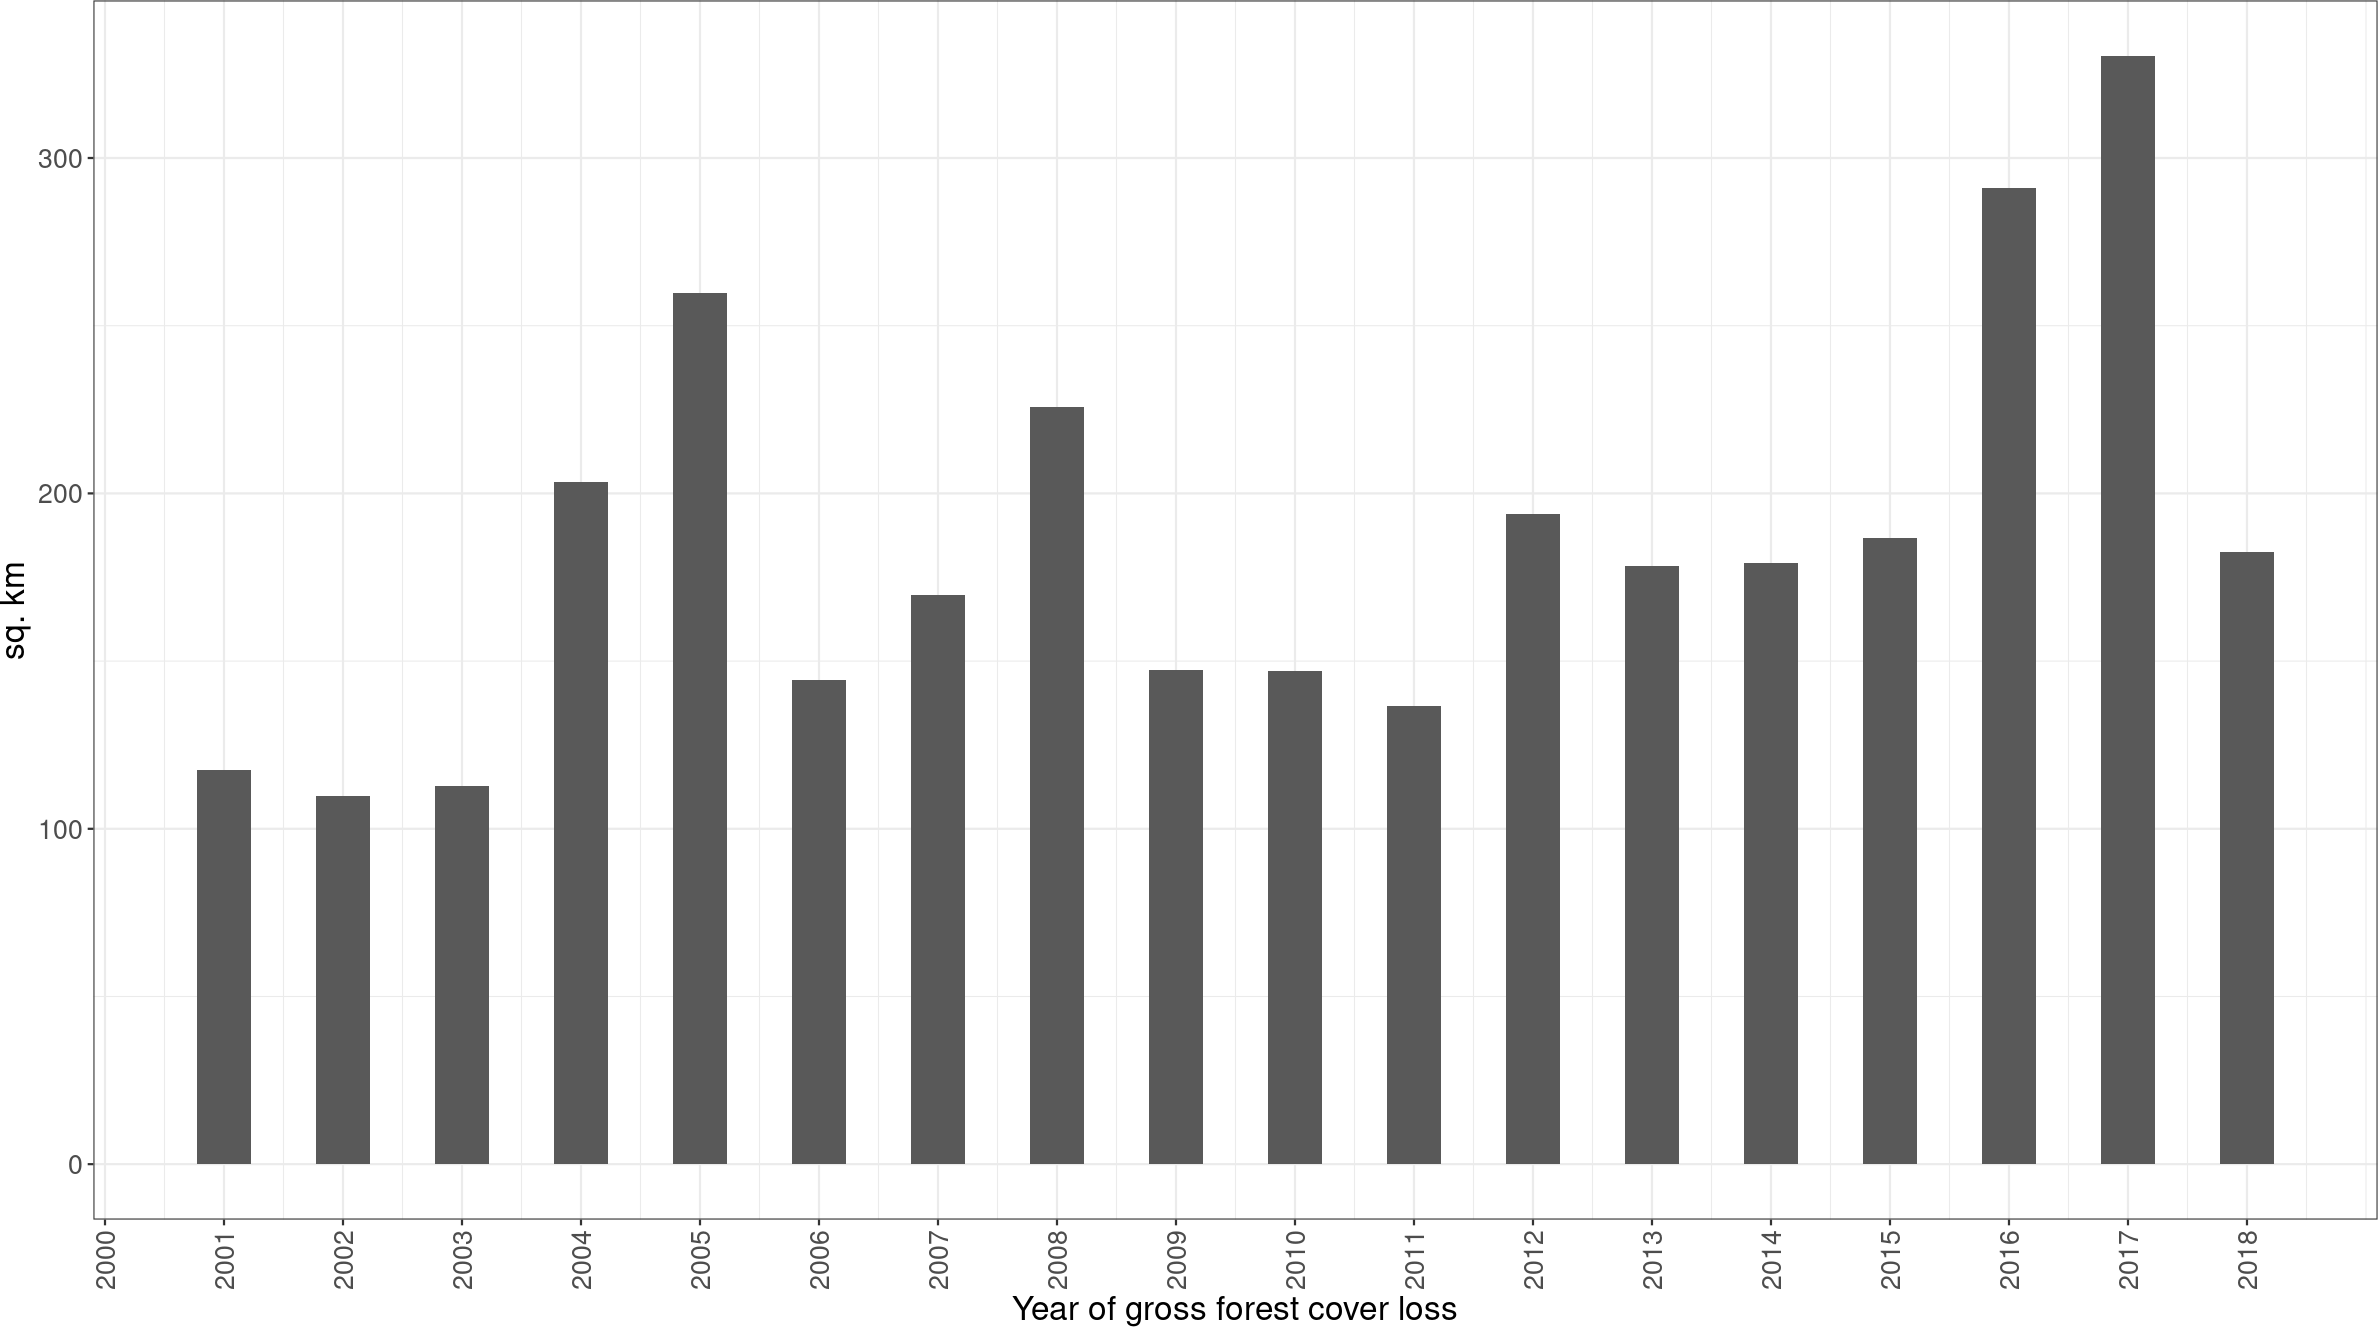
\includegraphics[width=0.5\linewidth]{img/data-download-preparation-eda/year-of-gross-forest-cover-loss-nationwide-by-year-1} \end{center}

\begin{itemize}
\tightlist
\item
  By 4-year periods
\end{itemize}

\begin{Shaded}
\begin{Highlighting}[]
\NormalTok{lysum }\SpecialCharTok{\%\textgreater{}\%}\NormalTok{ dplyr}\SpecialCharTok{::}\FunctionTok{filter}\NormalTok{(}\StringTok{\textasciigrave{}}\AttributeTok{Year of gross forest cover loss}\StringTok{\textasciigrave{}}\SpecialCharTok{\textgreater{}}\DecValTok{2000}\NormalTok{) }\SpecialCharTok{\%\textgreater{}\%} 
  \FunctionTok{mutate}\NormalTok{(}\StringTok{\textasciigrave{}}\AttributeTok{Period of gross forest cover loss}\StringTok{\textasciigrave{}} \OtherTok{=} \FunctionTok{case\_when}\NormalTok{(}
    \StringTok{\textasciigrave{}}\AttributeTok{Year of gross forest cover loss}\StringTok{\textasciigrave{}} \SpecialCharTok{\textless{}=} \DecValTok{2004} \SpecialCharTok{\textasciitilde{}} \StringTok{\textquotesingle{}2001{-}2004\textquotesingle{}}\NormalTok{,}
    \StringTok{\textasciigrave{}}\AttributeTok{Year of gross forest cover loss}\StringTok{\textasciigrave{}} \SpecialCharTok{\textgreater{}=} \DecValTok{2005} \SpecialCharTok{\&}
      \StringTok{\textasciigrave{}}\AttributeTok{Year of gross forest cover loss}\StringTok{\textasciigrave{}} \SpecialCharTok{\textless{}=} \DecValTok{2008} \SpecialCharTok{\textasciitilde{}} \StringTok{\textquotesingle{}2005{-}2008\textquotesingle{}}\NormalTok{,}
    \StringTok{\textasciigrave{}}\AttributeTok{Year of gross forest cover loss}\StringTok{\textasciigrave{}} \SpecialCharTok{\textgreater{}=} \DecValTok{2009} \SpecialCharTok{\&}
      \StringTok{\textasciigrave{}}\AttributeTok{Year of gross forest cover loss}\StringTok{\textasciigrave{}} \SpecialCharTok{\textless{}=} \DecValTok{2012} \SpecialCharTok{\textasciitilde{}} \StringTok{\textquotesingle{}2009{-}2012\textquotesingle{}}\NormalTok{,}
    \StringTok{\textasciigrave{}}\AttributeTok{Year of gross forest cover loss}\StringTok{\textasciigrave{}} \SpecialCharTok{\textgreater{}=} \DecValTok{2013} \SpecialCharTok{\&}
      \StringTok{\textasciigrave{}}\AttributeTok{Year of gross forest cover loss}\StringTok{\textasciigrave{}} \SpecialCharTok{\textless{}=} \DecValTok{2016} \SpecialCharTok{\textasciitilde{}} \StringTok{\textquotesingle{}2013{-}2016\textquotesingle{}}\NormalTok{,}
    \StringTok{\textasciigrave{}}\AttributeTok{Year of gross forest cover loss}\StringTok{\textasciigrave{}} \SpecialCharTok{\textgreater{}=} \DecValTok{2017} \SpecialCharTok{\textasciitilde{}} \StringTok{\textquotesingle{}2017{-}2018\textquotesingle{}}\NormalTok{)) }\SpecialCharTok{\%\textgreater{}\%} 
  \FunctionTok{group\_by}\NormalTok{(}\StringTok{\textasciigrave{}}\AttributeTok{Period of gross forest cover loss}\StringTok{\textasciigrave{}}\NormalTok{) }\SpecialCharTok{\%\textgreater{}\%}
  \FunctionTok{summarise\_each}\NormalTok{(}\FunctionTok{funs}\NormalTok{(}\FunctionTok{sum}\NormalTok{(.)), (}\StringTok{\textasciigrave{}}\AttributeTok{sq. km}\StringTok{\textasciigrave{}}\SpecialCharTok{:}\NormalTok{pct)) }\SpecialCharTok{\%\textgreater{}\%} 
  \FunctionTok{ggplot}\NormalTok{() }\SpecialCharTok{+} \FunctionTok{aes}\NormalTok{(}\AttributeTok{x =} \StringTok{\textasciigrave{}}\AttributeTok{Period of gross forest cover loss}\StringTok{\textasciigrave{}}\NormalTok{, }\AttributeTok{y =} \StringTok{\textasciigrave{}}\AttributeTok{sq. km}\StringTok{\textasciigrave{}}\NormalTok{) }\SpecialCharTok{+}
  \FunctionTok{theme\_bw}\NormalTok{() }\SpecialCharTok{+} \FunctionTok{geom\_col}\NormalTok{(}\AttributeTok{width =} \FloatTok{0.45}\NormalTok{) }\SpecialCharTok{+}
  \FunctionTok{theme}\NormalTok{(}\AttributeTok{axis.text.x =} \FunctionTok{element\_text}\NormalTok{(}\AttributeTok{angle =} \DecValTok{90}\NormalTok{, }\AttributeTok{vjust =} \FloatTok{0.5}\NormalTok{), }\AttributeTok{text =} \FunctionTok{element\_text}\NormalTok{(}\AttributeTok{size =} \DecValTok{16}\NormalTok{))}
\end{Highlighting}
\end{Shaded}

\begin{center}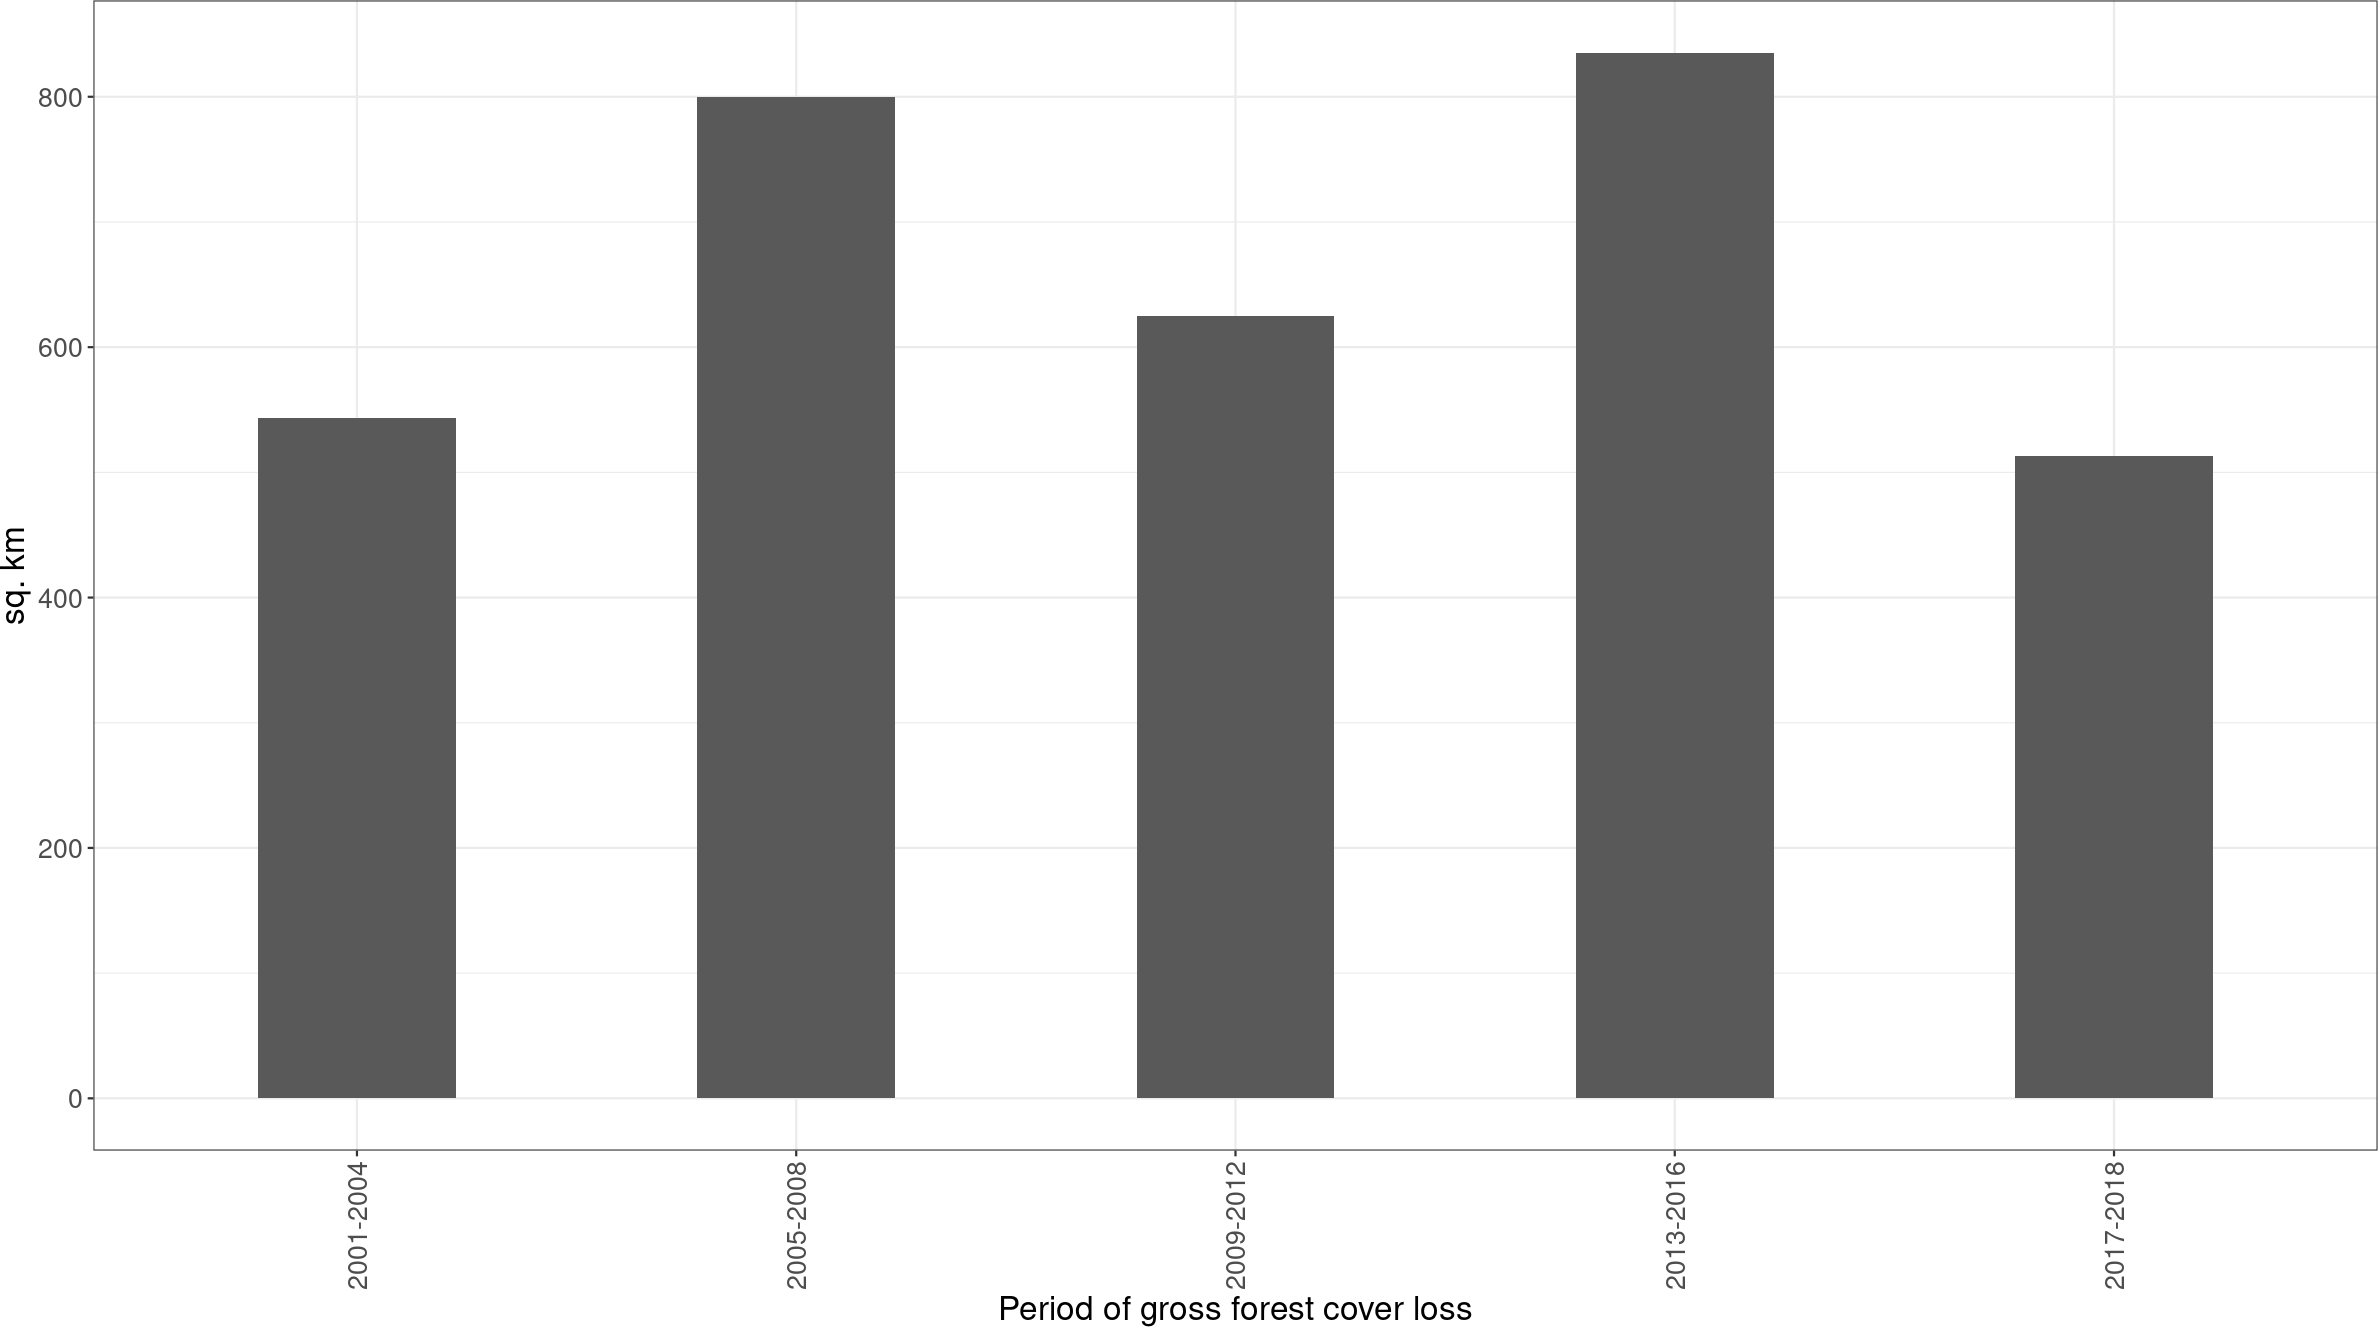
\includegraphics[width=0.5\linewidth]{img/data-download-preparation-eda/year-of-gross-forest-cover-loss-nationwide-by-period-1} \end{center}

\hypertarget{zonal-by-provinces}{%
\subsection{Zonal, by provinces}\label{zonal-by-provinces}}

\begin{Shaded}
\begin{Highlighting}[]
\CommentTok{\#Zonal statistics object}
\NormalTok{provzonal }\OtherTok{\textless{}{-}} \FunctionTok{readRDS}\NormalTok{(}\StringTok{\textquotesingle{}out/prov\_zonal\_statistics.RDS\textquotesingle{}}\NormalTok{)}

\CommentTok{\# Tree cover for pctc threshold}
\NormalTok{provzonal }\SpecialCharTok{\%\textgreater{}\%} \FunctionTok{select}\NormalTok{(}\FunctionTok{matches}\NormalTok{(}\StringTok{\textquotesingle{}\^{}TREECOVER2000\textquotesingle{}}\NormalTok{)) }\SpecialCharTok{\%\textgreater{}\%}
  \FunctionTok{gather}\NormalTok{(variable, value, }\SpecialCharTok{{-}}\NormalTok{geom) }\SpecialCharTok{\%\textgreater{}\%}
  \FunctionTok{tm\_shape}\NormalTok{() }\SpecialCharTok{+}
    \FunctionTok{tm\_fill}\NormalTok{(}\AttributeTok{col=}\StringTok{\textquotesingle{}value\textquotesingle{}}\NormalTok{, }\AttributeTok{palette =} \StringTok{"YlOrBr"}\NormalTok{, }\AttributeTok{size =} \FloatTok{0.1}\NormalTok{, }\AttributeTok{style =} \StringTok{\textquotesingle{}jenks\textquotesingle{}}\NormalTok{) }\SpecialCharTok{+}
    \FunctionTok{tm\_borders}\NormalTok{(}\AttributeTok{col =} \StringTok{\textquotesingle{}grey15\textquotesingle{}}\NormalTok{, }\AttributeTok{lwd =} \FloatTok{0.3}\NormalTok{) }\SpecialCharTok{+}
    \FunctionTok{tm\_facets}\NormalTok{(}\AttributeTok{by =} \StringTok{"variable"}\NormalTok{, }\AttributeTok{ncol =} \DecValTok{2}\NormalTok{, }\AttributeTok{nrow =} \DecValTok{2}\NormalTok{, }\AttributeTok{free.coords =} \ConstantTok{FALSE}\NormalTok{, }\AttributeTok{free.scales =} \ConstantTok{TRUE}\NormalTok{) }\SpecialCharTok{+}
    \FunctionTok{tm\_layout}\NormalTok{(}\AttributeTok{panel.label.size =} \DecValTok{1}\NormalTok{, }\AttributeTok{legend.title.size =} \DecValTok{1}\NormalTok{, }\AttributeTok{legend.text.size =} \DecValTok{1}\NormalTok{)}
\end{Highlighting}
\end{Shaded}

\begin{center}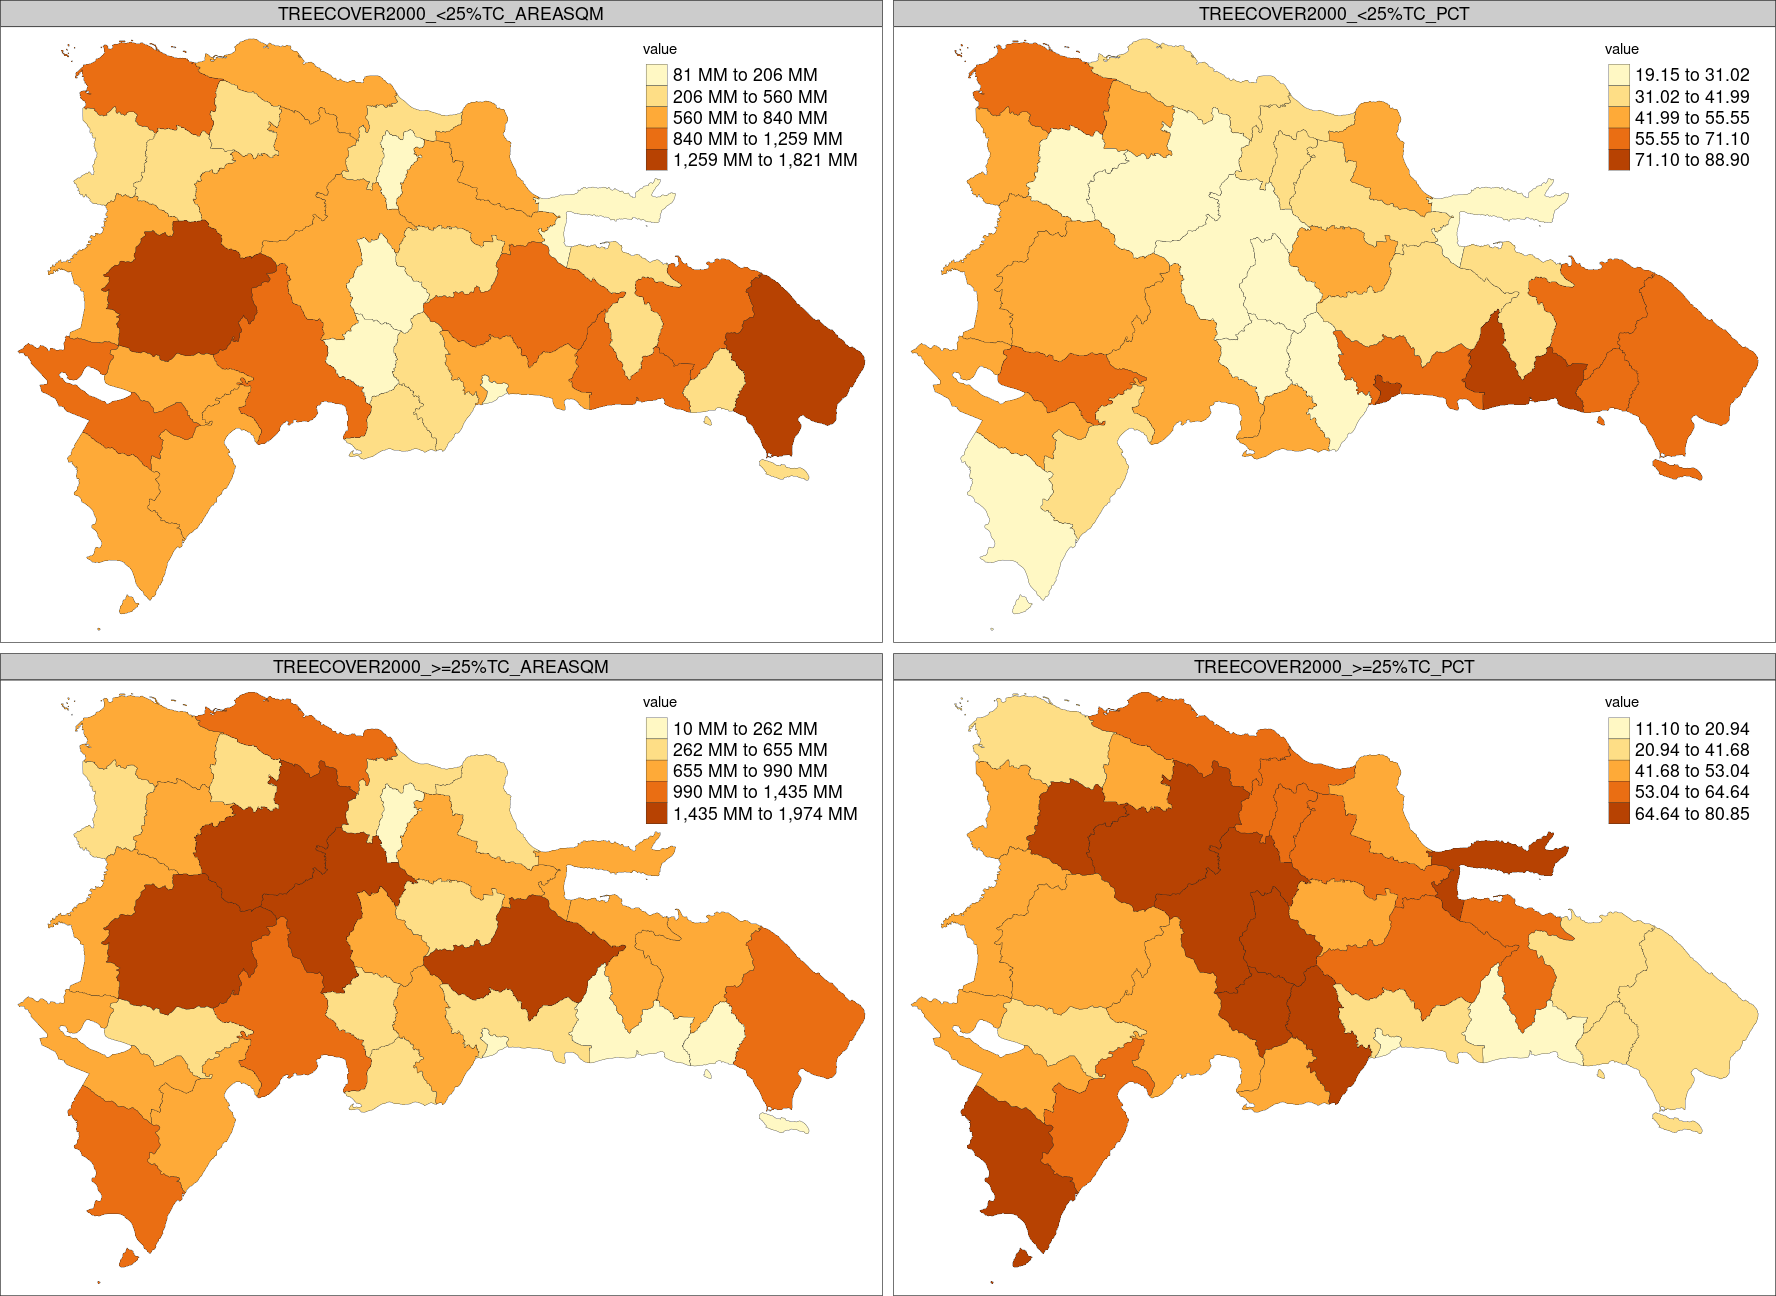
\includegraphics{img/data-download-preparation-eda/zonal-prov-1} \end{center}

\begin{Shaded}
\begin{Highlighting}[]
\CommentTok{\# Top twenty sorted descending by column 2}
\FunctionTok{stripped\_table}\NormalTok{(provzonal }\SpecialCharTok{\%\textgreater{}\%} \FunctionTok{select}\NormalTok{(TOPONIMIA, }\FunctionTok{matches}\NormalTok{(}\StringTok{\textquotesingle{}\^{}TREECOVER2000\textquotesingle{}}\NormalTok{)))}
\end{Highlighting}
\end{Shaded}

\begin{table}[H]
\centering
\begin{tabular}[t]{llrrrr}
\toprule
  & TOPONIMIA & TREECOVER2000\_>=25\%TC\_PCT & TREECOVER2000\_<25\%TC\_PCT & TREECOVER2000\_>=25\%TC\_AREASQM & TREECOVER2000\_<25\%TC\_AREASQM\\
\midrule
\cellcolor{lightgray}{1} & \cellcolor{lightgray}{SAMANÁ} & \cellcolor{lightgray}{80.85482} & \cellcolor{lightgray}{19.14518} & \cellcolor{lightgray}{697688722} & \cellcolor{lightgray}{165201971}\\
2 & MONSEÑOR NOUEL & 79.24722 & 20.75278 & 786118604 & 205863963\\
\cellcolor{lightgray}{3} & \cellcolor{lightgray}{SAN JOSÉ DE OCOA} & \cellcolor{lightgray}{76.76925} & \cellcolor{lightgray}{23.23075} & \cellcolor{lightgray}{655338410} & \cellcolor{lightgray}{198308635}\\
4 & SAN CRISTÓBAL & 73.34135 & 26.65865 & 909995521 & 330771898\\
\cellcolor{lightgray}{5} & \cellcolor{lightgray}{SANTIAGO RODRÍGUEZ} & \cellcolor{lightgray}{71.24034} & \cellcolor{lightgray}{28.75966} & \cellcolor{lightgray}{817955801} & \cellcolor{lightgray}{330208089}\\
\addlinespace
6 & SANTIAGO & 70.33967 & 29.66033 & 1974345122 & 832527766\\
\cellcolor{lightgray}{7} & \cellcolor{lightgray}{LA VEGA} & \cellcolor{lightgray}{69.57361} & \cellcolor{lightgray}{30.42639} & \cellcolor{lightgray}{1595092664} & \cellcolor{lightgray}{697576339}\\
8 & PEDERNALES & 68.98473 & 31.01527 & 1434924143 & 645136293\\
\cellcolor{lightgray}{9} & \cellcolor{lightgray}{HATO MAYOR} & \cellcolor{lightgray}{64.64493} & \cellcolor{lightgray}{35.35507} & \cellcolor{lightgray}{851745302} & \cellcolor{lightgray}{465829547}\\
10 & MONTE PLATA & 62.66562 & 37.33438 & 1630805609 & 971587235\\
\addlinespace
\cellcolor{lightgray}{11} & \cellcolor{lightgray}{PUERTO PLATA} & \cellcolor{lightgray}{62.25984} & \cellcolor{lightgray}{37.74016} & \cellcolor{lightgray}{1124498325} & \cellcolor{lightgray}{681639068}\\
12 & BARAHONA & 59.64874 & 40.35126 & 990426487 & 670005055\\
\cellcolor{lightgray}{13} & \cellcolor{lightgray}{HERMANAS MIRABAL} & \cellcolor{lightgray}{58.42910} & \cellcolor{lightgray}{41.57090} & \cellcolor{lightgray}{249509302} & \cellcolor{lightgray}{177519888}\\
14 & ESPAILLAT & 58.12143 & 41.87857 & 489330733 & 352580341\\
\cellcolor{lightgray}{15} & \cellcolor{lightgray}{DUARTE} & \cellcolor{lightgray}{58.01404} & \cellcolor{lightgray}{41.98596} & \cellcolor{lightgray}{956931584} & \cellcolor{lightgray}{692551115}\\
\addlinespace
16 & AZUA & 53.04008 & 46.95992 & 1422559629 & 1259486713\\
\cellcolor{lightgray}{17} & \cellcolor{lightgray}{SAN JUAN} & \cellcolor{lightgray}{52.85447} & \cellcolor{lightgray}{47.14553} & \cellcolor{lightgray}{1778257738} & \cellcolor{lightgray}{1586183858}\\
18 & DAJABÓN & 52.80924 & 47.19076 & 539049686 & 481699091\\
\cellcolor{lightgray}{19} & \cellcolor{lightgray}{SANCHEZ RAMÍREZ} & \cellcolor{lightgray}{52.80050} & \cellcolor{lightgray}{47.19950} & \cellcolor{lightgray}{626044975} & \cellcolor{lightgray}{559635063}\\
20 & ELÍAS PIÑA & 52.62086 & 47.37914 & 734376775 & 661223287\\
\bottomrule
\end{tabular}
\end{table}

\begin{Shaded}
\begin{Highlighting}[]

\CommentTok{\# Loss year}
\CommentTok{\# * PCT}
\NormalTok{provzonal }\SpecialCharTok{\%\textgreater{}\%} \FunctionTok{select}\NormalTok{(}\FunctionTok{matches}\NormalTok{(}\StringTok{\textquotesingle{}\^{}LOSSYEAR\_[1{-}9].*\_PCT$\textquotesingle{}}\NormalTok{)) }\SpecialCharTok{\%\textgreater{}\%}
  \FunctionTok{gather}\NormalTok{(variable, value, }\SpecialCharTok{{-}}\NormalTok{geom) }\SpecialCharTok{\%\textgreater{}\%}
  \FunctionTok{mutate}\NormalTok{(}\AttributeTok{variable =} \FunctionTok{factor}\NormalTok{(variable, }\AttributeTok{levels =} \FunctionTok{unique}\NormalTok{(variable))) }\SpecialCharTok{\%\textgreater{}\%} 
  \FunctionTok{tm\_shape}\NormalTok{() }\SpecialCharTok{+}
    \FunctionTok{tm\_fill}\NormalTok{(}\AttributeTok{col=}\StringTok{\textquotesingle{}value\textquotesingle{}}\NormalTok{, }\AttributeTok{palette =} \StringTok{"YlOrBr"}\NormalTok{, }\AttributeTok{size =} \FloatTok{0.1}\NormalTok{, }\AttributeTok{style =} \StringTok{\textquotesingle{}jenks\textquotesingle{}}\NormalTok{) }\SpecialCharTok{+}
    \FunctionTok{tm\_borders}\NormalTok{(}\AttributeTok{col =} \StringTok{\textquotesingle{}grey15\textquotesingle{}}\NormalTok{, }\AttributeTok{lwd =} \FloatTok{0.3}\NormalTok{) }\SpecialCharTok{+}
    \FunctionTok{tm\_facets}\NormalTok{(}\AttributeTok{by =} \StringTok{"variable"}\NormalTok{, }\AttributeTok{ncol =} \DecValTok{5}\NormalTok{, }\AttributeTok{nrow =} \DecValTok{4}\NormalTok{, }\AttributeTok{free.coords =} \ConstantTok{FALSE}\NormalTok{, }\AttributeTok{free.scales =} \ConstantTok{TRUE}\NormalTok{) }\SpecialCharTok{+}
    \FunctionTok{tm\_layout}\NormalTok{(}\AttributeTok{panel.label.size =} \DecValTok{1}\NormalTok{, }\AttributeTok{legend.title.size =} \DecValTok{1}\NormalTok{, }\AttributeTok{legend.text.size =} \FloatTok{0.75}\NormalTok{)}
\end{Highlighting}
\end{Shaded}

\begin{center}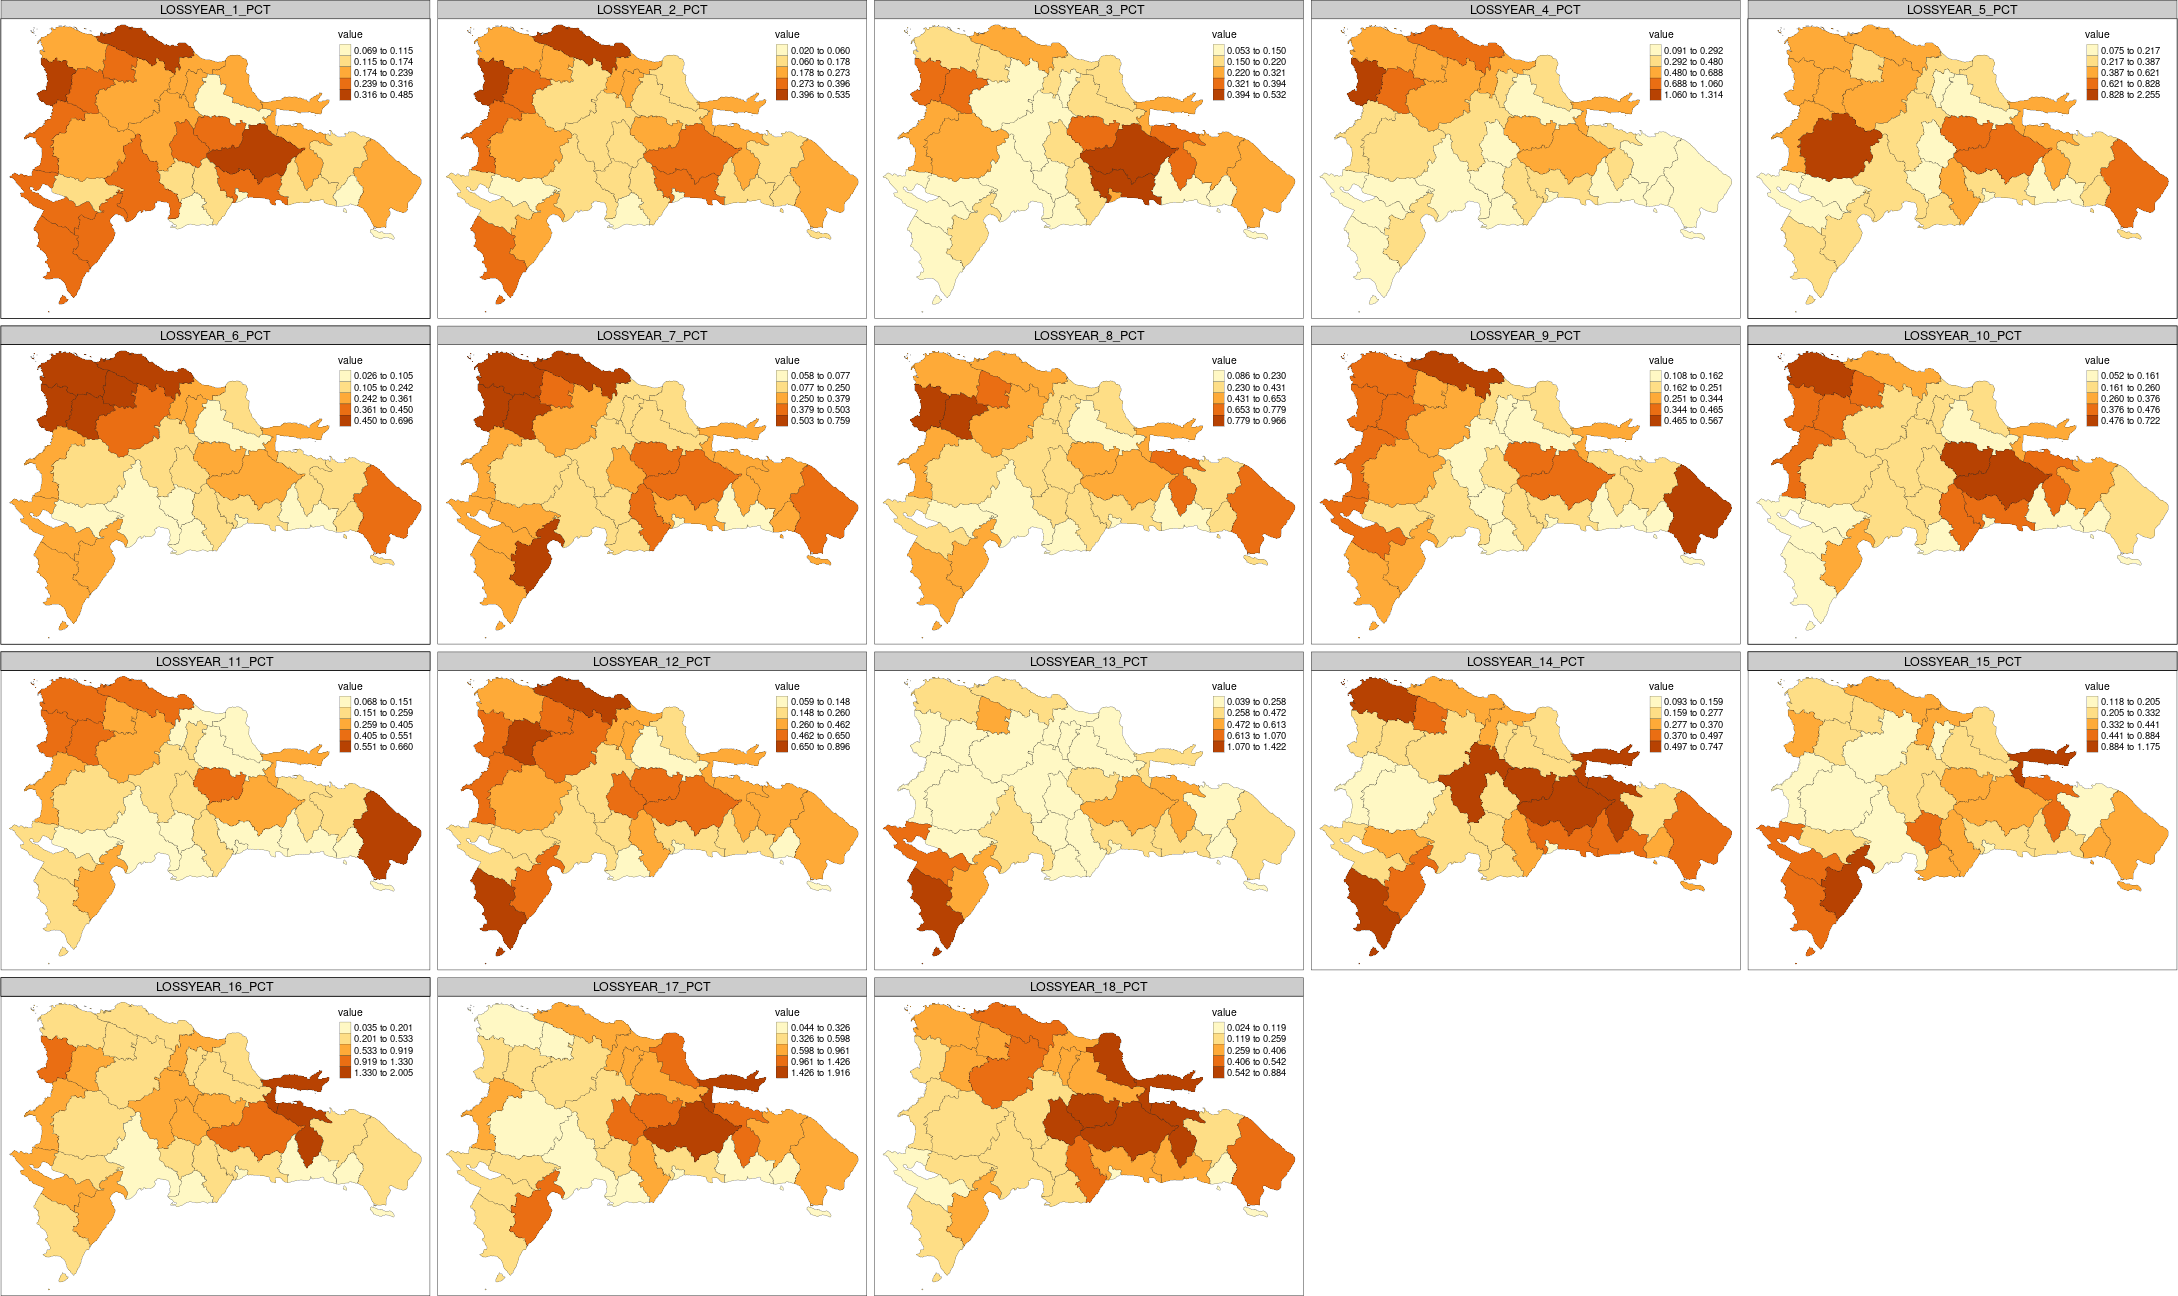
\includegraphics{img/data-download-preparation-eda/zonal-prov-2} \end{center}

\begin{Shaded}
\begin{Highlighting}[]
\CommentTok{\# Top twenty sorted descending by column 2}
\FunctionTok{stripped\_table}\NormalTok{(provzonal }\SpecialCharTok{\%\textgreater{}\%} \FunctionTok{select}\NormalTok{(TOPONIMIA, }\FunctionTok{matches}\NormalTok{(}\StringTok{\textquotesingle{}\^{}LOSSYEAR\_[1{-}9].*\_PCT$\textquotesingle{}}\NormalTok{)))}
\end{Highlighting}
\end{Shaded}

\begin{table}[H]
\centering
\resizebox{\linewidth}{!}{
\begin{tabular}[t]{llrrrrrrrrrrrrrrrrrr}
\toprule
  & TOPONIMIA & LOSSYEAR\_1\_PCT & LOSSYEAR\_2\_PCT & LOSSYEAR\_3\_PCT & LOSSYEAR\_4\_PCT & LOSSYEAR\_5\_PCT & LOSSYEAR\_6\_PCT & LOSSYEAR\_7\_PCT & LOSSYEAR\_8\_PCT & LOSSYEAR\_9\_PCT & LOSSYEAR\_10\_PCT & LOSSYEAR\_11\_PCT & LOSSYEAR\_12\_PCT & LOSSYEAR\_13\_PCT & LOSSYEAR\_14\_PCT & LOSSYEAR\_15\_PCT & LOSSYEAR\_16\_PCT & LOSSYEAR\_17\_PCT & LOSSYEAR\_18\_PCT\\
\midrule
\cellcolor{lightgray}{1} & \cellcolor{lightgray}{PUERTO PLATA} & \cellcolor{lightgray}{0.4854033} & \cellcolor{lightgray}{0.5351371} & \cellcolor{lightgray}{0.3030461} & \cellcolor{lightgray}{0.9500740} & \cellcolor{lightgray}{0.5055249} & \cellcolor{lightgray}{0.6957841} & \cellcolor{lightgray}{0.5974570} & \cellcolor{lightgray}{0.6533006} & \cellcolor{lightgray}{0.5522852} & \cellcolor{lightgray}{0.2971400} & \cellcolor{lightgray}{0.4568094} & \cellcolor{lightgray}{0.7188384} & \cellcolor{lightgray}{0.3663436} & \cellcolor{lightgray}{0.3215384} & \cellcolor{lightgray}{0.4078903} & \cellcolor{lightgray}{0.4661778} & \cellcolor{lightgray}{0.7320356} & \cellcolor{lightgray}{0.4957085}\\
2 & MONTE PLATA & 0.4039418 & 0.3434452 & 0.5319174 & 0.5990856 & 0.8280679 & 0.3364909 & 0.4261050 & 0.5998771 & 0.4211296 & 0.7218597 & 0.3840966 & 0.5049202 & 0.5338398 & 0.6051635 & 0.4013127 & 1.3295957 & 1.7683654 & 0.8837021\\
\cellcolor{lightgray}{3} & \cellcolor{lightgray}{DAJABÓN} & \cellcolor{lightgray}{0.3859482} & \cellcolor{lightgray}{0.4994623} & \cellcolor{lightgray}{0.3857320} & \cellcolor{lightgray}{1.3138814} & \cellcolor{lightgray}{0.5642555} & \cellcolor{lightgray}{0.6333730} & \cellcolor{lightgray}{0.7586350} & \cellcolor{lightgray}{0.9663479} & \cellcolor{lightgray}{0.4653721} & \cellcolor{lightgray}{0.4743090} & \cellcolor{lightgray}{0.5288679} & \cellcolor{lightgray}{0.5945260} & \cellcolor{lightgray}{0.1581270} & \cellcolor{lightgray}{0.2243617} & \cellcolor{lightgray}{0.4136240} & \cellcolor{lightgray}{1.3073949} & \cellcolor{lightgray}{0.5980575} & \cellcolor{lightgray}{0.2201814}\\
4 & SANCHEZ RAMÍREZ & 0.3155063 & 0.2208855 & 0.3544095 & 0.5350888 & 0.6887159 & 0.3173057 & 0.5028247 & 0.5889452 & 0.3766842 & 0.5659880 & 0.4704985 & 0.5568671 & 0.3777390 & 0.7467294 & 0.3760017 & 0.6270417 & 1.0814081 & 0.7779388\\
\cellcolor{lightgray}{5} & \cellcolor{lightgray}{BARAHONA} & \cellcolor{lightgray}{0.2998575} & \cellcolor{lightgray}{0.2703060} & \cellcolor{lightgray}{0.2199753} & \cellcolor{lightgray}{0.3992784} & \cellcolor{lightgray}{0.3350358} & \cellcolor{lightgray}{0.3610873} & \cellcolor{lightgray}{0.5961263} & \cellcolor{lightgray}{0.5263456} & \cellcolor{lightgray}{0.3440741} & \cellcolor{lightgray}{0.3436310} & \cellcolor{lightgray}{0.3990568} & \cellcolor{lightgray}{0.6184561} & \cellcolor{lightgray}{0.5691888} & \cellcolor{lightgray}{0.4556789} & \cellcolor{lightgray}{1.0650967} & \cellcolor{lightgray}{0.6482735} & \cellcolor{lightgray}{1.3546311} & \cellcolor{lightgray}{0.3753093}\\
\addlinespace
6 & MONSEÑOR NOUEL & 0.2824113 & 0.1507726 & 0.1862965 & 0.2836721 & 0.2126243 & 0.1842200 & 0.3424089 & 0.4217629 & 0.2037989 & 0.2141075 & 0.2493348 & 0.5413130 & 0.1340119 & 0.2562319 & 0.2707678 & 0.9194683 & 1.2140422 & 0.7173010\\
\cellcolor{lightgray}{7} & \cellcolor{lightgray}{SANTIAGO RODRÍGUEZ} & \cellcolor{lightgray}{0.2736038} & \cellcolor{lightgray}{0.3961808} & \cellcolor{lightgray}{0.3497259} & \cellcolor{lightgray}{1.0600704} & \cellcolor{lightgray}{0.4575014} & \cellcolor{lightgray}{0.5693137} & \cellcolor{lightgray}{0.5800144} & \cellcolor{lightgray}{0.8622043} & \cellcolor{lightgray}{0.3819560} & \cellcolor{lightgray}{0.4693554} & \cellcolor{lightgray}{0.5423378} & \cellcolor{lightgray}{0.7058593} & \cellcolor{lightgray}{0.1944061} & \cellcolor{lightgray}{0.2270847} & \cellcolor{lightgray}{0.3113444} & \cellcolor{lightgray}{0.7409728} & \cellcolor{lightgray}{0.5158745} & \cellcolor{lightgray}{0.3121133}\\
8 & INDEPENDENCIA & 0.2711904 & 0.1089000 & 0.1474574 & 0.2677834 & 0.1403110 & 0.3065486 & 0.2943748 & 0.3793840 & 0.3731932 & 0.1135119 & 0.2082021 & 0.2052521 & 1.0699287 & 0.1967346 & 0.8844539 & 0.6789524 & 0.3517540 & 0.1188717\\
\cellcolor{lightgray}{9} & \cellcolor{lightgray}{AZUA} & \cellcolor{lightgray}{0.2701846} & \cellcolor{lightgray}{0.1700380} & \cellcolor{lightgray}{0.1122706} & \cellcolor{lightgray}{0.1476552} & \cellcolor{lightgray}{0.2497767} & \cellcolor{lightgray}{0.0937280} & \cellcolor{lightgray}{0.2104697} & \cellcolor{lightgray}{0.1600261} & \cellcolor{lightgray}{0.2511208} & \cellcolor{lightgray}{0.2280522} & \cellcolor{lightgray}{0.0995157} & \cellcolor{lightgray}{0.1711078} & \cellcolor{lightgray}{0.4719864} & \cellcolor{lightgray}{0.2066843} & \cellcolor{lightgray}{0.2048191} & \cellcolor{lightgray}{0.1874834} & \cellcolor{lightgray}{0.2329348} & \cellcolor{lightgray}{0.1510016}\\
10 & SANTO DOMINGO & 0.2655681 & 0.3163866 & 0.4769824 & 0.4041745 & 0.3869900 & 0.1863160 & 0.3616090 & 0.2981847 & 0.2011263 & 0.4078488 & 0.1434113 & 0.2302381 & 0.3510948 & 0.4365084 & 0.2905534 & 0.3616655 & 0.5426678 & 0.3521688\\
\addlinespace
\cellcolor{lightgray}{11} & \cellcolor{lightgray}{VALVERDE} & \cellcolor{lightgray}{0.2611979} & \cellcolor{lightgray}{0.2553856} & \cellcolor{lightgray}{0.1753540} & \cellcolor{lightgray}{0.5959891} & \cellcolor{lightgray}{0.2612874} & \cellcolor{lightgray}{0.5922335} & \cellcolor{lightgray}{0.4354789} & \cellcolor{lightgray}{0.7788545} & \cellcolor{lightgray}{0.2929423} & \cellcolor{lightgray}{0.4686540} & \cellcolor{lightgray}{0.3940771} & \cellcolor{lightgray}{0.6503569} & \cellcolor{lightgray}{0.6132473} & \cellcolor{lightgray}{0.4969110} & \cellcolor{lightgray}{0.2831954} & \cellcolor{lightgray}{0.4157169} & \cellcolor{lightgray}{0.2378591} & \cellcolor{lightgray}{0.3705595}\\
12 & PEDERNALES & 0.2607003 & 0.3339835 & 0.1316057 & 0.2915415 & 0.2447845 & 0.2928501 & 0.3791489 & 0.5344514 & 0.3382631 & 0.1614212 & 0.1706524 & 0.8962699 & 1.4223744 & 0.6685683 & 0.6581700 & 0.4487539 & 0.3943927 & 0.1971433\\
\cellcolor{lightgray}{13} & \cellcolor{lightgray}{ELÍAS PIÑA} & \cellcolor{lightgray}{0.2534464} & \cellcolor{lightgray}{0.3174933} & \cellcolor{lightgray}{0.3209197} & \cellcolor{lightgray}{0.4796927} & \cellcolor{lightgray}{0.5114789} & \cellcolor{lightgray}{0.3298810} & \cellcolor{lightgray}{0.2870776} & \cellcolor{lightgray}{0.5510140} & \cellcolor{lightgray}{0.3946658} & \cellcolor{lightgray}{0.4270846} & \cellcolor{lightgray}{0.4050504} & \cellcolor{lightgray}{0.5805863} & \cellcolor{lightgray}{0.0637306} & \cellcolor{lightgray}{0.1014734} & \cellcolor{lightgray}{0.1503388} & \cellcolor{lightgray}{0.7099978} & \cellcolor{lightgray}{0.7971332} & \cellcolor{lightgray}{0.1848662}\\
14 & SANTIAGO & 0.2385887 & 0.1776507 & 0.1409831 & 0.5236214 & 0.6205194 & 0.3952453 & 0.3488538 & 0.5477083 & 0.2863432 & 0.2289697 & 0.3224604 & 0.5212101 & 0.1757898 & 0.2382218 & 0.1588320 & 0.3998058 & 0.4230540 & 0.5417849\\
\cellcolor{lightgray}{15} & \cellcolor{lightgray}{SAN JUAN} & \cellcolor{lightgray}{0.2371836} & \cellcolor{lightgray}{0.2004045} & \cellcolor{lightgray}{0.2609741} & \cellcolor{lightgray}{0.3329798} & \cellcolor{lightgray}{2.2552452} & \cellcolor{lightgray}{0.1875471} & \cellcolor{lightgray}{0.2504127} & \cellcolor{lightgray}{0.3398458} & \cellcolor{lightgray}{0.3150932} & \cellcolor{lightgray}{0.2595091} & \cellcolor{lightgray}{0.1693107} & \cellcolor{lightgray}{0.3840813} & \cellcolor{lightgray}{0.1896463} & \cellcolor{lightgray}{0.1592740} & \cellcolor{lightgray}{0.1317662} & \cellcolor{lightgray}{0.3455967} & \cellcolor{lightgray}{0.3258296} & \cellcolor{lightgray}{0.2154485}\\
\addlinespace
16 & HERMANAS MIRABAL & 0.2270777 & 0.2651537 & 0.1335245 & 0.4107385 & 0.2105379 & 0.3142563 & 0.2108825 & 0.3275226 & 0.1616077 & 0.1917584 & 0.2198416 & 0.3094322 & 0.1193967 & 0.2770417 & 0.1807318 & 0.5185918 & 0.7267176 & 0.3337250\\
\cellcolor{lightgray}{17} & \cellcolor{lightgray}{LA VEGA} & \cellcolor{lightgray}{0.2215651} & \cellcolor{lightgray}{0.1126597} & \cellcolor{lightgray}{0.0835562} & \cellcolor{lightgray}{0.3951270} & \cellcolor{lightgray}{0.3431451} & \cellcolor{lightgray}{0.1919161} & \cellcolor{lightgray}{0.1580316} & \cellcolor{lightgray}{0.2788415} & \cellcolor{lightgray}{0.1133335} & \cellcolor{lightgray}{0.1772841} & \cellcolor{lightgray}{0.1705137} & \cellcolor{lightgray}{0.2238754} & \cellcolor{lightgray}{0.0601001} & \cellcolor{lightgray}{0.5803689} & \cellcolor{lightgray}{0.3087151} & \cellcolor{lightgray}{0.6971679} & \cellcolor{lightgray}{0.4252573} & \cellcolor{lightgray}{0.1800116}\\
18 & MONTE CRISTI & 0.2206413 & 0.2545229 & 0.2071980 & 0.6881459 & 0.4269014 & 0.6814243 & 0.5968959 & 0.6485977 & 0.4370619 & 0.5796620 & 0.5505089 & 0.3745352 & 0.3531979 & 0.7201909 & 0.3214656 & 0.5196754 & 0.2361948 & 0.4062284\\
\cellcolor{lightgray}{19} & \cellcolor{lightgray}{LA ALTAGRACIA} & \cellcolor{lightgray}{0.2194468} & \cellcolor{lightgray}{0.2731973} & \cellcolor{lightgray}{0.2878811} & \cellcolor{lightgray}{0.2329765} & \cellcolor{lightgray}{0.7061977} & \cellcolor{lightgray}{0.4499186} & \cellcolor{lightgray}{0.5029080} & \cellcolor{lightgray}{0.7617653} & \cellcolor{lightgray}{0.5668980} & \cellcolor{lightgray}{0.2265677} & \cellcolor{lightgray}{0.6604766} & \cellcolor{lightgray}{0.3419018} & \cellcolor{lightgray}{0.4177518} & \cellcolor{lightgray}{0.4235467} & \cellcolor{lightgray}{0.4413736} & \cellcolor{lightgray}{0.5330860} & \cellcolor{lightgray}{0.7415321} & \cellcolor{lightgray}{0.5332578}\\
20 & MARÍA TRINIDAD SÁNCHEZ & 0.2186695 & 0.1393362 & 0.1892168 & 0.4124596 & 0.3075154 & 0.2367192 & 0.2088519 & 0.4097156 & 0.2200720 & 0.2120838 & 0.1359824 & 0.2602569 & 0.1933023 & 0.2573299 & 0.2494027 & 0.4291678 & 1.2977478 & 0.6553986\\
\bottomrule
\end{tabular}}
\end{table}

\begin{Shaded}
\begin{Highlighting}[]
\CommentTok{\# * AREASQM}
\NormalTok{provzonal }\SpecialCharTok{\%\textgreater{}\%} \FunctionTok{select}\NormalTok{(}\FunctionTok{matches}\NormalTok{(}\StringTok{\textquotesingle{}\^{}LOSSYEAR\_[1{-}9].*\_AREASQM$\textquotesingle{}}\NormalTok{)) }\SpecialCharTok{\%\textgreater{}\%}
  \FunctionTok{gather}\NormalTok{(variable, value, }\SpecialCharTok{{-}}\NormalTok{geom) }\SpecialCharTok{\%\textgreater{}\%}
  \FunctionTok{mutate}\NormalTok{(}\AttributeTok{variable =} \FunctionTok{factor}\NormalTok{(variable, }\AttributeTok{levels =} \FunctionTok{unique}\NormalTok{(variable))) }\SpecialCharTok{\%\textgreater{}\%} 
  \FunctionTok{tm\_shape}\NormalTok{() }\SpecialCharTok{+}
    \FunctionTok{tm\_fill}\NormalTok{(}\AttributeTok{col=}\StringTok{\textquotesingle{}value\textquotesingle{}}\NormalTok{, }\AttributeTok{palette =} \StringTok{"YlOrBr"}\NormalTok{, }\AttributeTok{size =} \FloatTok{0.1}\NormalTok{, }\AttributeTok{style =} \StringTok{\textquotesingle{}jenks\textquotesingle{}}\NormalTok{) }\SpecialCharTok{+}
    \FunctionTok{tm\_borders}\NormalTok{(}\AttributeTok{col =} \StringTok{\textquotesingle{}grey15\textquotesingle{}}\NormalTok{, }\AttributeTok{lwd =} \FloatTok{0.3}\NormalTok{) }\SpecialCharTok{+}
    \FunctionTok{tm\_facets}\NormalTok{(}\AttributeTok{by =} \StringTok{"variable"}\NormalTok{, }\AttributeTok{ncol =} \DecValTok{5}\NormalTok{, }\AttributeTok{nrow =} \DecValTok{4}\NormalTok{, }\AttributeTok{free.coords =} \ConstantTok{FALSE}\NormalTok{, }\AttributeTok{free.scales =} \ConstantTok{TRUE}\NormalTok{) }\SpecialCharTok{+}
    \FunctionTok{tm\_layout}\NormalTok{(}\AttributeTok{panel.label.size =} \DecValTok{1}\NormalTok{, }\AttributeTok{legend.title.size =} \DecValTok{1}\NormalTok{, }\AttributeTok{legend.text.size =} \FloatTok{0.75}\NormalTok{)}
\end{Highlighting}
\end{Shaded}

\begin{center}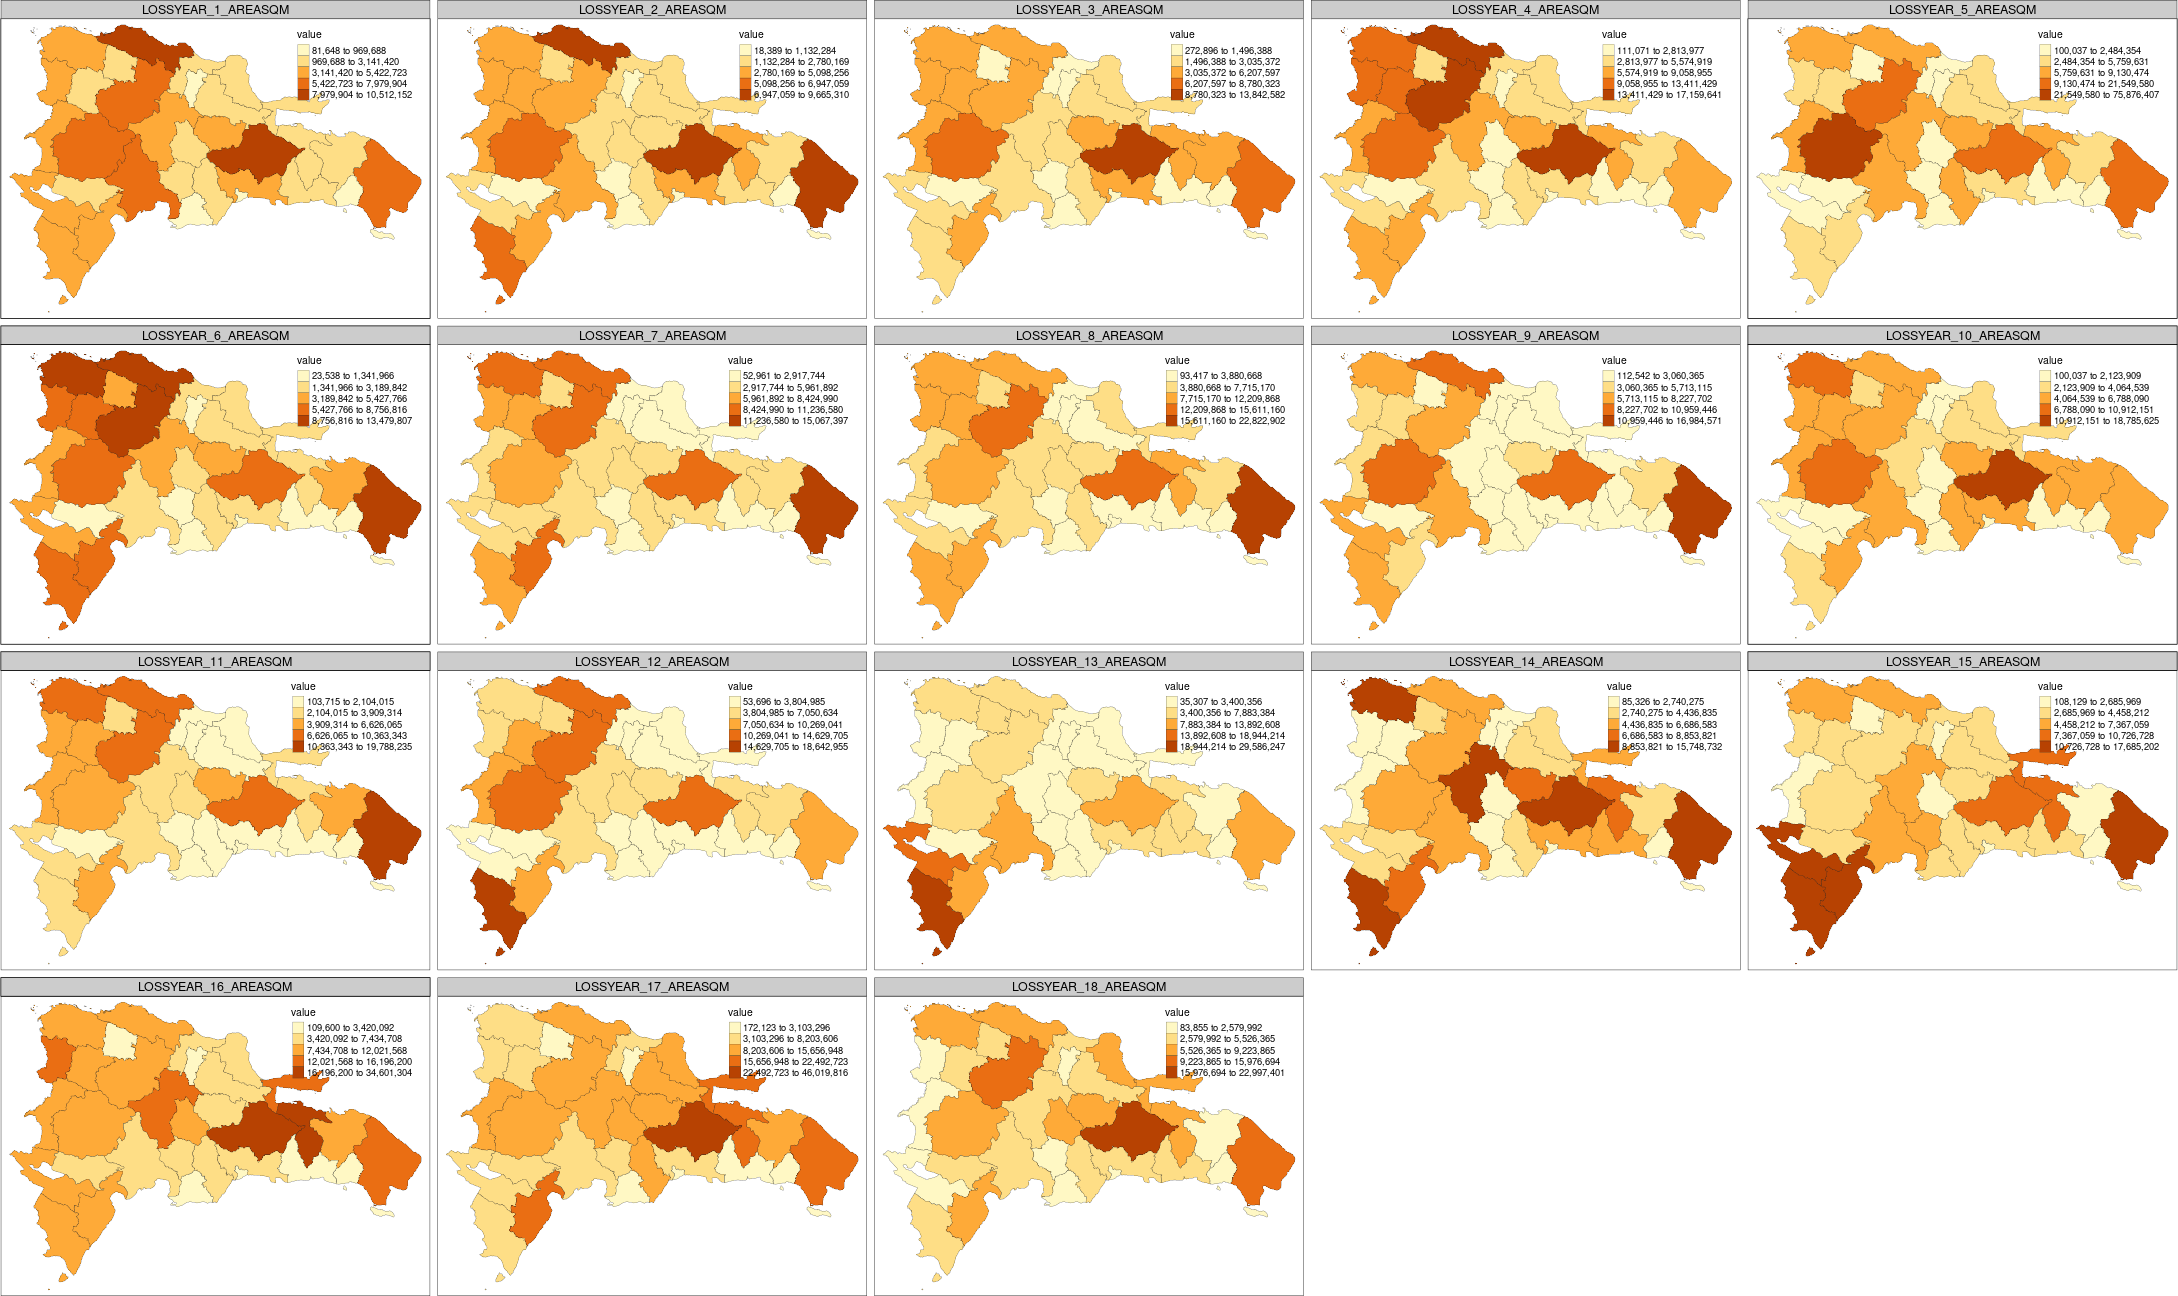
\includegraphics{img/data-download-preparation-eda/zonal-prov-3} \end{center}

\begin{Shaded}
\begin{Highlighting}[]
\CommentTok{\# Top twenty sorted descending by column 2}
\FunctionTok{stripped\_table}\NormalTok{(provzonal }\SpecialCharTok{\%\textgreater{}\%} \FunctionTok{select}\NormalTok{(TOPONIMIA, }\FunctionTok{matches}\NormalTok{(}\StringTok{\textquotesingle{}\^{}LOSSYEAR\_[1{-}9].*\_AREASQM$\textquotesingle{}}\NormalTok{)))}
\end{Highlighting}
\end{Shaded}

\begin{table}[H]
\centering
\resizebox{\linewidth}{!}{
\begin{tabular}[t]{llrrrrrrrrrrrrrrrrrr}
\toprule
  & TOPONIMIA & LOSSYEAR\_1\_AREASQM & LOSSYEAR\_2\_AREASQM & LOSSYEAR\_3\_AREASQM & LOSSYEAR\_4\_AREASQM & LOSSYEAR\_5\_AREASQM & LOSSYEAR\_6\_AREASQM & LOSSYEAR\_7\_AREASQM & LOSSYEAR\_8\_AREASQM & LOSSYEAR\_9\_AREASQM & LOSSYEAR\_10\_AREASQM & LOSSYEAR\_11\_AREASQM & LOSSYEAR\_12\_AREASQM & LOSSYEAR\_13\_AREASQM & LOSSYEAR\_14\_AREASQM & LOSSYEAR\_15\_AREASQM & LOSSYEAR\_16\_AREASQM & LOSSYEAR\_17\_AREASQM & LOSSYEAR\_18\_AREASQM\\
\midrule
\cellcolor{lightgray}{1} & \cellcolor{lightgray}{MONTE PLATA} & \cellcolor{lightgray}{10512152} & \cellcolor{lightgray}{8937794} & \cellcolor{lightgray}{13842582} & \cellcolor{lightgray}{15590561} & \cellcolor{lightgray}{21549580} & \cellcolor{lightgray}{8756816} & \cellcolor{lightgray}{11088926} & \cellcolor{lightgray}{15611160} & \cellcolor{lightgray}{10959446} & \cellcolor{lightgray}{18785625} & \cellcolor{lightgray}{9995703} & \cellcolor{lightgray}{13140006} & \cellcolor{lightgray}{13892608.0} & \cellcolor{lightgray}{15748732} & \cellcolor{lightgray}{10443733} & \cellcolor{lightgray}{34601304} & \cellcolor{lightgray}{46019816} & \cellcolor{lightgray}{22997401}\\
2 & PUERTO PLATA & 8767050 & 9665310 & 5473429 & 17159641 & 9130474 & 12566816 & 10790895 & 11799506 & 9975030 & 5366756 & 8250606 & 12983209 & 6616669.4 & 5807426 & 7367059 & 8419811 & 13221568 & 8953176\\
\cellcolor{lightgray}{3} & \cellcolor{lightgray}{SAN JUAN} & \cellcolor{lightgray}{7979904} & \cellcolor{lightgray}{6742493} & \cellcolor{lightgray}{8780323} & \cellcolor{lightgray}{11202912} & \cellcolor{lightgray}{75876407} & \cellcolor{lightgray}{6309914} & \cellcolor{lightgray}{8424990} & \cellcolor{lightgray}{11433915} & \cellcolor{lightgray}{10601127} & \cellcolor{lightgray}{8731032} & \cellcolor{lightgray}{5696358} & \cellcolor{lightgray}{12922192} & \cellcolor{lightgray}{6380539.4} & \cellcolor{lightgray}{5358682} & \cellcolor{lightgray}{4433199} & \cellcolor{lightgray}{11627398} & \cellcolor{lightgray}{10962345} & \cellcolor{lightgray}{7248640}\\
4 & AZUA & 7246475 & 4560498 & 3011150 & 3960180 & 6699127 & 2513828 & 5644894 & 4291973 & 6735176 & 6116467 & 2669057 & 4589189 & 12658893.6 & 5543370 & 5493343 & 5028392 & 6247418 & 4049934\\
\cellcolor{lightgray}{5} & \cellcolor{lightgray}{SANTIAGO} & \cellcolor{lightgray}{6696882} & \cellcolor{lightgray}{4986430} & \cellcolor{lightgray}{3957215} & \cellcolor{lightgray}{14697387} & \cellcolor{lightgray}{17417191} & \cellcolor{lightgray}{11094034} & \cellcolor{lightgray}{9791882} & \cellcolor{lightgray}{15373476} & \cellcolor{lightgray}{8037289} & \cellcolor{lightgray}{6426888} & \cellcolor{lightgray}{9051054} & \cellcolor{lightgray}{14629705} & \cellcolor{lightgray}{4934196.5} & \cellcolor{lightgray}{6686583} & \cellcolor{lightgray}{4458212} & \cellcolor{lightgray}{11222042} & \cellcolor{lightgray}{11874589} & \cellcolor{lightgray}{15207213}\\
\addlinespace
6 & LA ALTAGRACIA & 6574744 & 8185140 & 8625075 & 6980102 & 21158066 & 13479807 & 15067397 & 22822902 & 16984571 & 6788090 & 19788235 & 10243564 & 12516069.9 & 12689690 & 13223791 & 15971544 & 22216705 & 15976694\\
\cellcolor{lightgray}{7} & \cellcolor{lightgray}{PEDERNALES} & \cellcolor{lightgray}{5422723} & \cellcolor{lightgray}{6947059} & \cellcolor{lightgray}{2737478} & \cellcolor{lightgray}{6064239} & \cellcolor{lightgray}{5091665} & \cellcolor{lightgray}{6091459} & \cellcolor{lightgray}{7886527} & \cellcolor{lightgray}{11116913} & \cellcolor{lightgray}{7036077} & \cellcolor{lightgray}{3357659} & \cellcolor{lightgray}{3549673} & \cellcolor{lightgray}{18642955} & \cellcolor{lightgray}{29586246.8} & \cellcolor{lightgray}{13906625} & \cellcolor{lightgray}{13690334} & \cellcolor{lightgray}{9334352} & \cellcolor{lightgray}{8203606} & \cellcolor{lightgray}{4100700}\\
8 & LA VEGA & 5079754 & 2582913 & 1915667 & 9058955 & 7867181 & 4400001 & 3623141 & 6392912 & 2598362 & 4064539 & 3909314 & 5132721 & 1377897.0 & 13305938 & 7077815 & 15983752 & 9749743 & 4127070\\
\cellcolor{lightgray}{9} & \cellcolor{lightgray}{BARAHONA} & \cellcolor{lightgray}{4978929} & \cellcolor{lightgray}{4488245} & \cellcolor{lightgray}{3652539} & \cellcolor{lightgray}{6629744} & \cellcolor{lightgray}{5563041} & \cellcolor{lightgray}{5995607} & \cellcolor{lightgray}{9898269} & \cellcolor{lightgray}{8739609} & \cellcolor{lightgray}{5713115} & \cellcolor{lightgray}{5705758} & \cellcolor{lightgray}{6626065} & \cellcolor{lightgray}{10269041} & \cellcolor{lightgray}{9450989.6} & \cellcolor{lightgray}{7566236} & \cellcolor{lightgray}{17685202} & \cellcolor{lightgray}{10764138} & \cellcolor{lightgray}{22492723} & \cellcolor{lightgray}{6231753}\\
10 & INDEPENDENCIA & 4801712 & 1928189 & 2610889 & 4741387 & 2484354 & 5427766 & 5212215 & 6717394 & 6607779 & 2009848 & 3686438 & 3634205 & 18944213.5 & 3483393 & 15660187 & 12021568 & 6228174 & 2104749\\
\addlinespace
\cellcolor{lightgray}{11} & \cellcolor{lightgray}{MONTE CRISTI} & \cellcolor{lightgray}{4153577} & \cellcolor{lightgray}{4791400} & \cellcolor{lightgray}{3900507} & \cellcolor{lightgray}{12954363} & \cellcolor{lightgray}{8036428} & \cellcolor{lightgray}{12827829} & \cellcolor{lightgray}{11236580} & \cellcolor{lightgray}{12209868} & \cellcolor{lightgray}{8227702} & \cellcolor{lightgray}{10912151} & \cellcolor{lightgray}{10363343} & \cellcolor{lightgray}{7050634} & \cellcolor{lightgray}{6648959.9} & \cellcolor{lightgray}{13557610} & \cellcolor{lightgray}{6051598} & \cellcolor{lightgray}{9782902} & \cellcolor{lightgray}{4446372} & \cellcolor{lightgray}{7647260}\\
12 & DAJABÓN & 3939561 & 5098256 & 3937354 & 13411429 & 5759631 & 6465147 & 7743758 & 9863985 & 4750280 & 4841504 & 5398413 & 6068616 & 1614079.8 & 2290169 & 4222062 & 13345218 & 6104665 & 2247499\\
\cellcolor{lightgray}{13} & \cellcolor{lightgray}{SANCHEZ RAMÍREZ} & \cellcolor{lightgray}{3740896} & \cellcolor{lightgray}{2618995} & \cellcolor{lightgray}{4202163} & \cellcolor{lightgray}{6344442} & \cellcolor{lightgray}{8165967} & \cellcolor{lightgray}{3762230} & \cellcolor{lightgray}{5961892} & \cellcolor{lightgray}{6983005} & \cellcolor{lightgray}{4466269} & \cellcolor{lightgray}{6710807} & \cellcolor{lightgray}{5578606} & \cellcolor{lightgray}{6602663} & \cellcolor{lightgray}{4478775.5} & \cellcolor{lightgray}{8853821} & \cellcolor{lightgray}{4458177} & \cellcolor{lightgray}{7434708} & \cellcolor{lightgray}{12822040} & \cellcolor{lightgray}{9223865}\\
14 & ELÍAS PIÑA & 3537098 & 4430936 & 4478755 & 6694591 & 7138200 & 4603819 & 4006455 & 7689952 & 5507956 & 5960393 & 5652883 & 8102662 & 889424.2 & 1416163 & 2098129 & 9908730 & 11124792 & 2579992\\
\cellcolor{lightgray}{15} & \cellcolor{lightgray}{SANTO DOMINGO} & \cellcolor{lightgray}{3456185} & \cellcolor{lightgray}{4117554} & \cellcolor{lightgray}{6207597} & \cellcolor{lightgray}{5260052} & \cellcolor{lightgray}{5036408} & \cellcolor{lightgray}{2424774} & \cellcolor{lightgray}{4706091} & \cellcolor{lightgray}{3880668} & \cellcolor{lightgray}{2617519} & \cellcolor{lightgray}{5307870} & \cellcolor{lightgray}{1866399} & \cellcolor{lightgray}{2996390} & \cellcolor{lightgray}{4569256.2} & \cellcolor{lightgray}{5680856} & \cellcolor{lightgray}{3781352} & \cellcolor{lightgray}{4706827} & \cellcolor{lightgray}{7062447} & \cellcolor{lightgray}{4583234}\\
\addlinespace
16 & SANTIAGO RODRÍGUEZ & 3141420 & 4548805 & 4015426 & 12171346 & 5252866 & 6536654 & 6659516 & 9899518 & 4385481 & 5388969 & 6226927 & 8104421 & 2232100.1 & 2607305 & 3574744 & 8507583 & 5923084 & 3583573\\
\cellcolor{lightgray}{17} & \cellcolor{lightgray}{MONSEÑOR NOUEL} & \cellcolor{lightgray}{2801471} & \cellcolor{lightgray}{1495638} & \cellcolor{lightgray}{1848029} & \cellcolor{lightgray}{2813977} & \cellcolor{lightgray}{2109196} & \cellcolor{lightgray}{1827430} & \cellcolor{lightgray}{3396636} & \cellcolor{lightgray}{4183814} & \cellcolor{lightgray}{2021650} & \cellcolor{lightgray}{2123909} & \cellcolor{lightgray}{2473357} & \cellcolor{lightgray}{5369731} & \cellcolor{lightgray}{1329374.4} & \cellcolor{lightgray}{2541776} & \cellcolor{lightgray}{2685969} & \cellcolor{lightgray}{9120965} & \cellcolor{lightgray}{12043087} & \cellcolor{lightgray}{7115500}\\
18 & EL SEIBO & 2645538 & 2780169 & 5113774 & 4597320 & 5246934 & 3735093 & 5257969 & 7715170 & 4418548 & 5937010 & 4638519 & 5555188 & 3203925.5 & 4108823 & 2658780 & 7928520 & 11888734 & 2555784\\
\cellcolor{lightgray}{19} & \cellcolor{lightgray}{MARÍA TRINIDAD SÁNCHEZ} & \cellcolor{lightgray}{2638183} & \cellcolor{lightgray}{1681051} & \cellcolor{lightgray}{2282845} & \cellcolor{lightgray}{4976205} & \cellcolor{lightgray}{3710083} & \cellcolor{lightgray}{2855947} & \cellcolor{lightgray}{2519737} & \cellcolor{lightgray}{4943099} & \cellcolor{lightgray}{2655104} & \cellcolor{lightgray}{2558729} & \cellcolor{lightgray}{1640588} & \cellcolor{lightgray}{3139924} & \cellcolor{lightgray}{2332136.3} & \cellcolor{lightgray}{3104610} & \cellcolor{lightgray}{3008971} & \cellcolor{lightgray}{5177784} & \cellcolor{lightgray}{15656948} & \cellcolor{lightgray}{7907193}\\
20 & HATO MAYOR & 2563792 & 3420105 & 5190115 & 5891939 & 7558955 & 3189842 & 3473809 & 9824067 & 3060365 & 6267864 & 2582919 & 6084683 & 7883383.6 & 8226203 & 10726728 & 26411836 & 18794028 & 8975846\\
\bottomrule
\end{tabular}}
\end{table}

\begin{Shaded}
\begin{Highlighting}[]

\CommentTok{\# Total loss 2001{-}2018}
\NormalTok{provzonal }\SpecialCharTok{\%\textgreater{}\%} \FunctionTok{select}\NormalTok{(}\FunctionTok{matches}\NormalTok{(}\StringTok{\textquotesingle{}\^{}LOSS0118\textquotesingle{}}\NormalTok{)) }\SpecialCharTok{\%\textgreater{}\%} \FunctionTok{select}\NormalTok{(}\SpecialCharTok{{-}}\FunctionTok{matches}\NormalTok{(}\StringTok{\textquotesingle{}\textless{}NA\textgreater{}\textquotesingle{}}\NormalTok{)) }\SpecialCharTok{\%\textgreater{}\%} 
  \FunctionTok{gather}\NormalTok{(variable, value, }\SpecialCharTok{{-}}\NormalTok{geom) }\SpecialCharTok{\%\textgreater{}\%}
  \FunctionTok{mutate}\NormalTok{(}\AttributeTok{variable =} \FunctionTok{factor}\NormalTok{(variable, }\AttributeTok{levels =} \FunctionTok{unique}\NormalTok{(variable))) }\SpecialCharTok{\%\textgreater{}\%} 
  \FunctionTok{tm\_shape}\NormalTok{() }\SpecialCharTok{+}
    \FunctionTok{tm\_fill}\NormalTok{(}\AttributeTok{col=}\StringTok{\textquotesingle{}value\textquotesingle{}}\NormalTok{, }\AttributeTok{palette =} \StringTok{"YlOrBr"}\NormalTok{, }\AttributeTok{size =} \FloatTok{0.1}\NormalTok{, }\AttributeTok{style =} \StringTok{\textquotesingle{}jenks\textquotesingle{}}\NormalTok{) }\SpecialCharTok{+}
    \FunctionTok{tm\_borders}\NormalTok{(}\AttributeTok{col =} \StringTok{\textquotesingle{}grey15\textquotesingle{}}\NormalTok{, }\AttributeTok{lwd =} \FloatTok{0.3}\NormalTok{) }\SpecialCharTok{+}
    \FunctionTok{tm\_facets}\NormalTok{(}\AttributeTok{by =} \StringTok{"variable"}\NormalTok{, }\AttributeTok{ncol =} \DecValTok{2}\NormalTok{, }\AttributeTok{nrow =} \DecValTok{1}\NormalTok{, }\AttributeTok{free.coords =} \ConstantTok{FALSE}\NormalTok{, }\AttributeTok{free.scales =} \ConstantTok{TRUE}\NormalTok{) }\SpecialCharTok{+}
    \FunctionTok{tm\_layout}\NormalTok{(}\AttributeTok{panel.label.size =} \DecValTok{1}\NormalTok{, }\AttributeTok{legend.title.size =} \DecValTok{1}\NormalTok{, }\AttributeTok{legend.text.size =} \DecValTok{1}\NormalTok{)}
\end{Highlighting}
\end{Shaded}

\begin{center}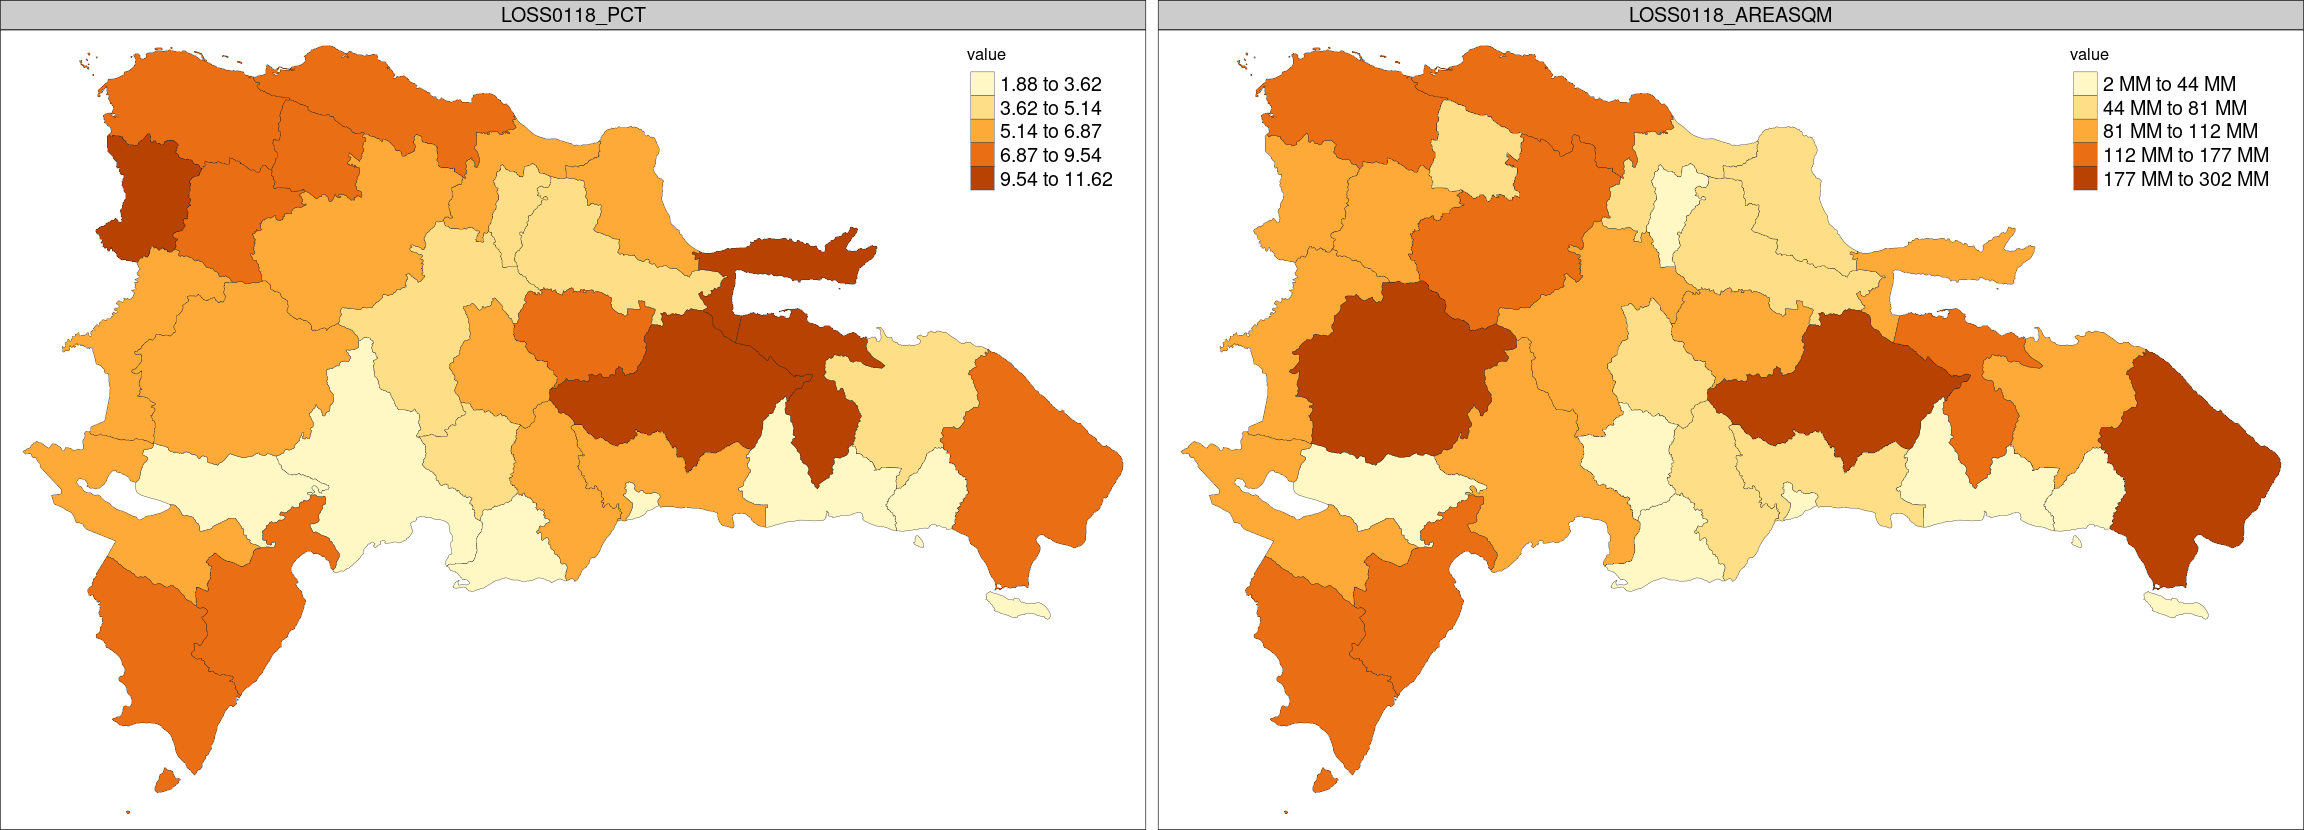
\includegraphics{img/data-download-preparation-eda/zonal-prov-4} \end{center}

\begin{Shaded}
\begin{Highlighting}[]
\CommentTok{\# Top twenty sorted descending by column 2}
\FunctionTok{stripped\_table}\NormalTok{(provzonal }\SpecialCharTok{\%\textgreater{}\%} \FunctionTok{select}\NormalTok{(TOPONIMIA, }\FunctionTok{matches}\NormalTok{(}\StringTok{\textquotesingle{}\^{}LOSS0118\textquotesingle{}}\NormalTok{)) }\SpecialCharTok{\%\textgreater{}\%} \FunctionTok{select}\NormalTok{(}\SpecialCharTok{{-}}\FunctionTok{matches}\NormalTok{(}\StringTok{\textquotesingle{}\textless{}NA\textgreater{}\textquotesingle{}}\NormalTok{)))}
\end{Highlighting}
\end{Shaded}

\begin{table}[H]
\centering
\begin{tabular}[t]{llrr}
\toprule
  & TOPONIMIA & LOSS0118\_PCT & LOSS0118\_AREASQM\\
\midrule
\cellcolor{lightgray}{1} & \cellcolor{lightgray}{MONTE PLATA} & \cellcolor{lightgray}{11.622916} & \cellcolor{lightgray}{302473946}\\
2 & SAMANÁ & 11.232321 & 96922649\\
\cellcolor{lightgray}{3} & \cellcolor{lightgray}{HATO MAYOR} & \cellcolor{lightgray}{10.635182} & \cellcolor{lightgray}{140126481}\\
4 & DAJABÓN & 10.492457 & 107101625\\
\cellcolor{lightgray}{5} & \cellcolor{lightgray}{PUERTO PLATA} & \cellcolor{lightgray}{9.540494} & \cellcolor{lightgray}{172314432}\\
\addlinespace
6 & SANCHEZ RAMÍREZ & 9.480578 & 112409320\\
\cellcolor{lightgray}{7} & \cellcolor{lightgray}{BARAHONA} & \cellcolor{lightgray}{9.181408} & \cellcolor{lightgray}{152451002}\\
8 & SANTIAGO RODRÍGUEZ & 8.949919 & 102759738\\
\cellcolor{lightgray}{9} & \cellcolor{lightgray}{LA ALTAGRACIA} & \cellcolor{lightgray}{8.320683} & \cellcolor{lightgray}{249292186}\\
10 & MONTE CRISTI & 8.223049 & 154799087\\
\addlinespace
\cellcolor{lightgray}{11} & \cellcolor{lightgray}{PEDERNALES} & \cellcolor{lightgray}{7.825075} & \cellcolor{lightgray}{162766292}\\
12 & VALVERDE & 7.579301 & 62354694\\
\cellcolor{lightgray}{13} & \cellcolor{lightgray}{ELÍAS PIÑA} & \cellcolor{lightgray}{6.865931} & \cellcolor{lightgray}{95820932}\\
14 & MONSEÑOR NOUEL & 6.784546 & 67301511\\
\cellcolor{lightgray}{15} & \cellcolor{lightgray}{SAN JUAN} & \cellcolor{lightgray}{6.560149} & \cellcolor{lightgray}{220712371}\\
\addlinespace
16 & SAN CRISTÓBAL & 6.542953 & 81182825\\
\cellcolor{lightgray}{17} & \cellcolor{lightgray}{SANTIAGO} & \cellcolor{lightgray}{6.289643} & \cellcolor{lightgray}{176542269}\\
18 & INDEPENDENCIA & 6.116804 & 108304461\\
\cellcolor{lightgray}{19} & \cellcolor{lightgray}{ESPAILLAT} & \cellcolor{lightgray}{6.052755} & \cellcolor{lightgray}{50958817}\\
20 & MARÍA TRINIDAD SÁNCHEZ & 6.033228 & 72789136\\
\bottomrule
\end{tabular}
\end{table}

\begin{Shaded}
\begin{Highlighting}[]

\CommentTok{\# Total loss 2012{-}2018}
\NormalTok{provzonal }\SpecialCharTok{\%\textgreater{}\%} \FunctionTok{select}\NormalTok{(}\FunctionTok{matches}\NormalTok{(}\StringTok{\textquotesingle{}\^{}LOSS1218\textquotesingle{}}\NormalTok{)) }\SpecialCharTok{\%\textgreater{}\%} \FunctionTok{select}\NormalTok{(}\SpecialCharTok{{-}}\FunctionTok{matches}\NormalTok{(}\StringTok{\textquotesingle{}\textless{}NA\textgreater{}\textquotesingle{}}\NormalTok{)) }\SpecialCharTok{\%\textgreater{}\%} 
  \FunctionTok{gather}\NormalTok{(variable, value, }\SpecialCharTok{{-}}\NormalTok{geom) }\SpecialCharTok{\%\textgreater{}\%}
  \FunctionTok{mutate}\NormalTok{(}\AttributeTok{variable =} \FunctionTok{factor}\NormalTok{(variable, }\AttributeTok{levels =} \FunctionTok{unique}\NormalTok{(variable))) }\SpecialCharTok{\%\textgreater{}\%} 
  \FunctionTok{tm\_shape}\NormalTok{() }\SpecialCharTok{+}
    \FunctionTok{tm\_fill}\NormalTok{(}\AttributeTok{col=}\StringTok{\textquotesingle{}value\textquotesingle{}}\NormalTok{, }\AttributeTok{palette =} \StringTok{"YlOrBr"}\NormalTok{, }\AttributeTok{size =} \FloatTok{0.1}\NormalTok{, }\AttributeTok{style =} \StringTok{\textquotesingle{}jenks\textquotesingle{}}\NormalTok{) }\SpecialCharTok{+}
    \FunctionTok{tm\_borders}\NormalTok{(}\AttributeTok{col =} \StringTok{\textquotesingle{}grey15\textquotesingle{}}\NormalTok{, }\AttributeTok{lwd =} \FloatTok{0.3}\NormalTok{) }\SpecialCharTok{+}
    \FunctionTok{tm\_facets}\NormalTok{(}\AttributeTok{by =} \StringTok{"variable"}\NormalTok{, }\AttributeTok{ncol =} \DecValTok{2}\NormalTok{, }\AttributeTok{nrow =} \DecValTok{1}\NormalTok{, }\AttributeTok{free.coords =} \ConstantTok{FALSE}\NormalTok{, }\AttributeTok{free.scales =} \ConstantTok{TRUE}\NormalTok{) }\SpecialCharTok{+}
    \FunctionTok{tm\_layout}\NormalTok{(}\AttributeTok{panel.label.size =} \DecValTok{1}\NormalTok{, }\AttributeTok{legend.title.size =} \DecValTok{1}\NormalTok{, }\AttributeTok{legend.text.size =} \DecValTok{1}\NormalTok{)}
\end{Highlighting}
\end{Shaded}

\begin{center}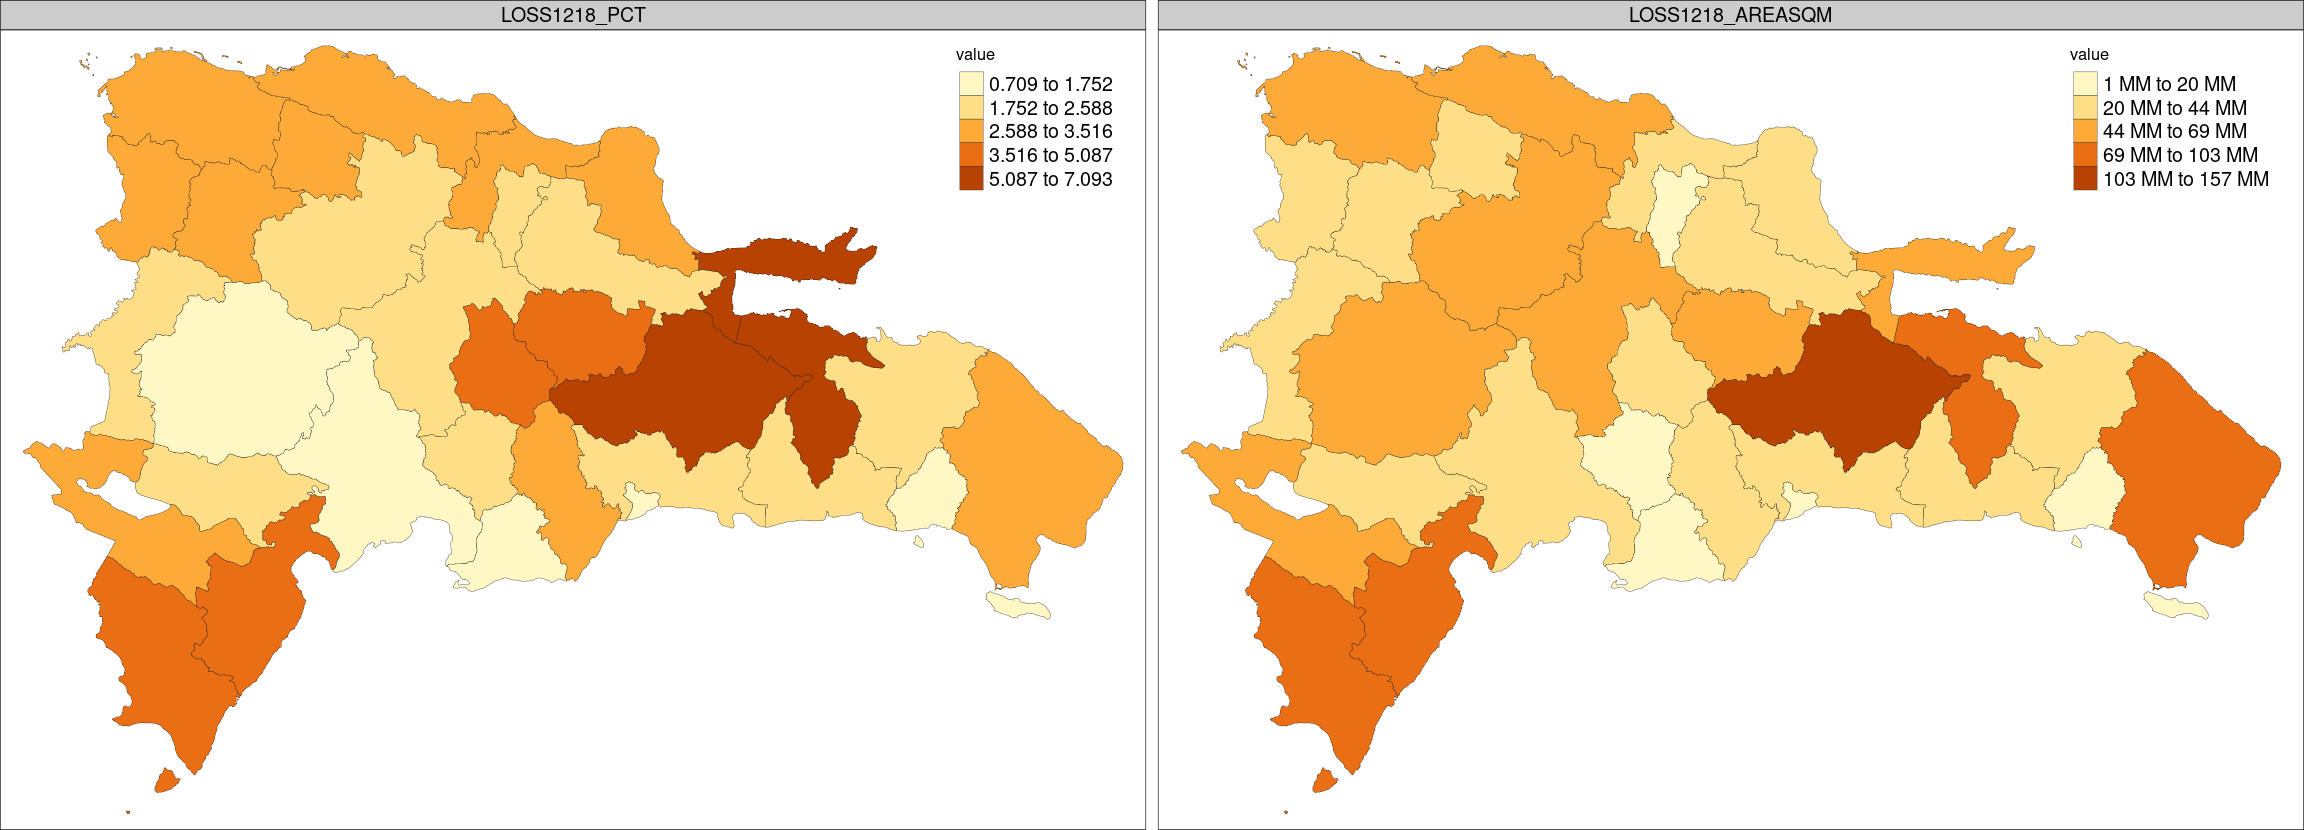
\includegraphics{img/data-download-preparation-eda/zonal-prov-5} \end{center}

\begin{Shaded}
\begin{Highlighting}[]
\CommentTok{\# Top twenty sorted descending by column 2}
\FunctionTok{stripped\_table}\NormalTok{(provzonal }\SpecialCharTok{\%\textgreater{}\%} \FunctionTok{select}\NormalTok{(TOPONIMIA, }\FunctionTok{matches}\NormalTok{(}\StringTok{\textquotesingle{}\^{}LOSS1218\textquotesingle{}}\NormalTok{)) }\SpecialCharTok{\%\textgreater{}\%} \FunctionTok{select}\NormalTok{(}\SpecialCharTok{{-}}\FunctionTok{matches}\NormalTok{(}\StringTok{\textquotesingle{}\textless{}NA\textgreater{}\textquotesingle{}}\NormalTok{)))}
\end{Highlighting}
\end{Shaded}

\begin{table}[H]
\centering
\begin{tabular}[t]{llrr}
\toprule
  & TOPONIMIA & LOSS1218\_PCT & LOSS1218\_AREASQM\\
\midrule
\cellcolor{lightgray}{1} & \cellcolor{lightgray}{SAMANÁ} & \cellcolor{lightgray}{7.092585} & \cellcolor{lightgray}{61201256}\\
2 & HATO MAYOR & 6.610836 & 87102708\\
\cellcolor{lightgray}{3} & \cellcolor{lightgray}{MONTE PLATA} & \cellcolor{lightgray}{6.026899} & \cellcolor{lightgray}{156843601}\\
4 & BARAHONA & 5.086634 & 84460081\\
\cellcolor{lightgray}{5} & \cellcolor{lightgray}{PEDERNALES} & \cellcolor{lightgray}{4.685672} & \cellcolor{lightgray}{97464819}\\
\addlinespace
6 & SANCHEZ RAMÍREZ & 4.543726 & 53874049\\
\cellcolor{lightgray}{7} & \cellcolor{lightgray}{MONSEÑOR NOUEL} & \cellcolor{lightgray}{4.053136} & \cellcolor{lightgray}{40206403}\\
8 & DAJABÓN & 3.516272 & 35892309\\
\cellcolor{lightgray}{9} & \cellcolor{lightgray}{PUERTO PLATA} & \cellcolor{lightgray}{3.508532} & \cellcolor{lightgray}{63368918}\\
10 & INDEPENDENCIA & 3.505947 & 62076489\\
\addlinespace
\cellcolor{lightgray}{11} & \cellcolor{lightgray}{LA ALTAGRACIA} & \cellcolor{lightgray}{3.432450} & \cellcolor{lightgray}{102838057}\\
12 & MARÍA TRINIDAD SÁNCHEZ & 3.342606 & 40327565\\
\cellcolor{lightgray}{13} & \cellcolor{lightgray}{ESPAILLAT} & \cellcolor{lightgray}{3.308128} & \cellcolor{lightgray}{27851494}\\
14 & SAN CRISTÓBAL & 3.174297 & 39385647\\
\cellcolor{lightgray}{15} & \cellcolor{lightgray}{VALVERDE} & \cellcolor{lightgray}{3.067846} & \cellcolor{lightgray}{25239085}\\
\addlinespace
16 & SANTIAGO RODRÍGUEZ & 3.007655 & 34532810\\
\cellcolor{lightgray}{17} & \cellcolor{lightgray}{MONTE CRISTI} & \cellcolor{lightgray}{2.931488} & \cellcolor{lightgray}{55185337}\\
18 & ELÍAS PIÑA & 2.588126 & 36119894\\
\cellcolor{lightgray}{19} & \cellcolor{lightgray}{SANTO DOMINGO} & \cellcolor{lightgray}{2.564897} & \cellcolor{lightgray}{33380362}\\
20 & LA VEGA & 2.475496 & 56754936\\
\bottomrule
\end{tabular}
\end{table}

\begin{Shaded}
\begin{Highlighting}[]

\CommentTok{\# Fires M6}
\NormalTok{provzonal }\SpecialCharTok{\%\textgreater{}\%} \FunctionTok{select}\NormalTok{(}\FunctionTok{matches}\NormalTok{(}\StringTok{\textquotesingle{}\^{}LOSS0118|NFIRESM6\textquotesingle{}}\NormalTok{)) }\SpecialCharTok{\%\textgreater{}\%} \FunctionTok{select}\NormalTok{(}\SpecialCharTok{{-}}\FunctionTok{matches}\NormalTok{(}\StringTok{\textquotesingle{}\textless{}NA\textgreater{}\textquotesingle{}}\NormalTok{)) }\SpecialCharTok{\%\textgreater{}\%} 
  \FunctionTok{gather}\NormalTok{(variable, value, }\SpecialCharTok{{-}}\NormalTok{geom) }\SpecialCharTok{\%\textgreater{}\%}
  \FunctionTok{mutate}\NormalTok{(}\AttributeTok{variable =} \FunctionTok{factor}\NormalTok{(variable, }\AttributeTok{levels =} \FunctionTok{unique}\NormalTok{(variable))) }\SpecialCharTok{\%\textgreater{}\%} 
  \FunctionTok{tm\_shape}\NormalTok{() }\SpecialCharTok{+}
  \FunctionTok{tm\_fill}\NormalTok{(}\AttributeTok{col=}\StringTok{\textquotesingle{}value\textquotesingle{}}\NormalTok{, }\AttributeTok{palette =} \StringTok{"YlOrBr"}\NormalTok{, }\AttributeTok{size =} \FloatTok{0.1}\NormalTok{, }\AttributeTok{style =} \StringTok{\textquotesingle{}jenks\textquotesingle{}}\NormalTok{) }\SpecialCharTok{+}
  \FunctionTok{tm\_borders}\NormalTok{(}\AttributeTok{col =} \StringTok{\textquotesingle{}grey15\textquotesingle{}}\NormalTok{, }\AttributeTok{lwd =} \FloatTok{0.3}\NormalTok{) }\SpecialCharTok{+}
  \FunctionTok{tm\_facets}\NormalTok{(}\AttributeTok{by =} \StringTok{"variable"}\NormalTok{, }\AttributeTok{ncol =} \DecValTok{3}\NormalTok{, }\AttributeTok{nrow =} \DecValTok{1}\NormalTok{, }\AttributeTok{free.coords =} \ConstantTok{FALSE}\NormalTok{, }\AttributeTok{free.scales =} \ConstantTok{TRUE}\NormalTok{) }\SpecialCharTok{+}
  \FunctionTok{tm\_layout}\NormalTok{(}\AttributeTok{panel.label.size =} \DecValTok{1}\NormalTok{, }\AttributeTok{legend.title.size =} \DecValTok{1}\NormalTok{, }\AttributeTok{legend.text.size =} \DecValTok{1}\NormalTok{)}
\end{Highlighting}
\end{Shaded}

\begin{center}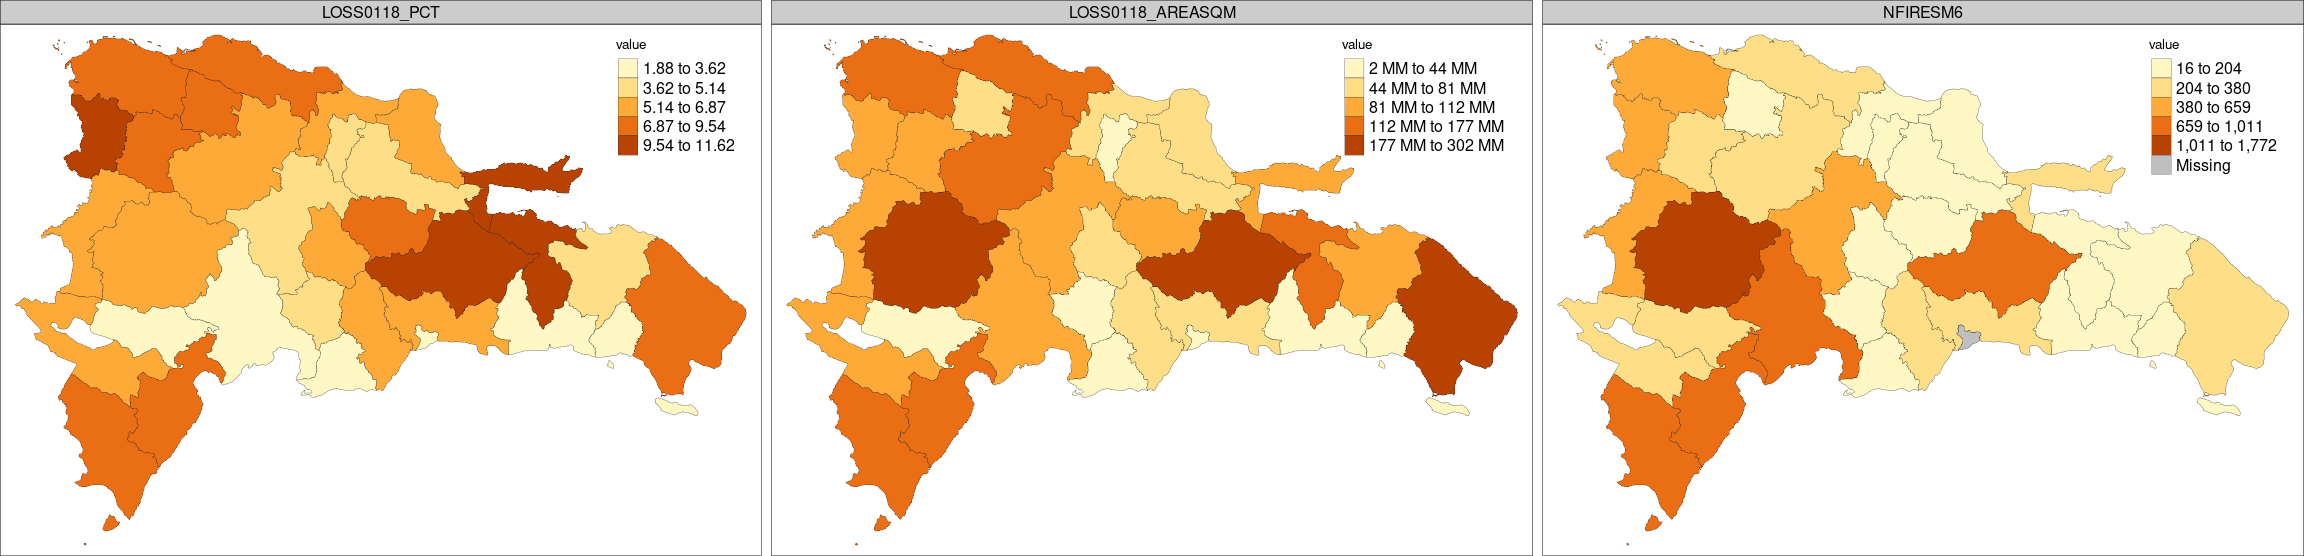
\includegraphics{img/data-download-preparation-eda/zonal-prov-6} \end{center}

\begin{Shaded}
\begin{Highlighting}[]
\CommentTok{\# Top twenty sorted descending by column 2}
\FunctionTok{stripped\_table}\NormalTok{(provzonal }\SpecialCharTok{\%\textgreater{}\%} \FunctionTok{select}\NormalTok{(TOPONIMIA, }\FunctionTok{matches}\NormalTok{(}\StringTok{\textquotesingle{}\^{}LOSS0118|NFIRESM6\textquotesingle{}}\NormalTok{)) }\SpecialCharTok{\%\textgreater{}\%} \FunctionTok{select}\NormalTok{(}\SpecialCharTok{{-}}\FunctionTok{matches}\NormalTok{(}\StringTok{\textquotesingle{}\textless{}NA\textgreater{}\textquotesingle{}}\NormalTok{)))}
\end{Highlighting}
\end{Shaded}

\begin{table}[H]
\centering
\begin{tabular}[t]{llrrr}
\toprule
  & TOPONIMIA & LOSS0118\_PCT & LOSS0118\_AREASQM & NFIRESM6\\
\midrule
\cellcolor{lightgray}{1} & \cellcolor{lightgray}{MONTE PLATA} & \cellcolor{lightgray}{11.622916} & \cellcolor{lightgray}{302473946} & \cellcolor{lightgray}{791}\\
2 & SAMANÁ & 11.232321 & 96922649 & 248\\
\cellcolor{lightgray}{3} & \cellcolor{lightgray}{HATO MAYOR} & \cellcolor{lightgray}{10.635182} & \cellcolor{lightgray}{140126481} & \cellcolor{lightgray}{193}\\
4 & DAJABÓN & 10.492457 & 107101625 & 444\\
\cellcolor{lightgray}{5} & \cellcolor{lightgray}{PUERTO PLATA} & \cellcolor{lightgray}{9.540494} & \cellcolor{lightgray}{172314432} & \cellcolor{lightgray}{289}\\
\addlinespace
6 & SANCHEZ RAMÍREZ & 9.480578 & 112409320 & 204\\
\cellcolor{lightgray}{7} & \cellcolor{lightgray}{BARAHONA} & \cellcolor{lightgray}{9.181408} & \cellcolor{lightgray}{152451002} & \cellcolor{lightgray}{1006}\\
8 & SANTIAGO RODRÍGUEZ & 8.949919 & 102759738 & 349\\
\cellcolor{lightgray}{9} & \cellcolor{lightgray}{LA ALTAGRACIA} & \cellcolor{lightgray}{8.320683} & \cellcolor{lightgray}{249292186} & \cellcolor{lightgray}{230}\\
10 & MONTE CRISTI & 8.223049 & 154799087 & 554\\
\addlinespace
\cellcolor{lightgray}{11} & \cellcolor{lightgray}{PEDERNALES} & \cellcolor{lightgray}{7.825075} & \cellcolor{lightgray}{162766292} & \cellcolor{lightgray}{1011}\\
12 & VALVERDE & 7.579301 & 62354694 & 183\\
\cellcolor{lightgray}{13} & \cellcolor{lightgray}{ELÍAS PIÑA} & \cellcolor{lightgray}{6.865931} & \cellcolor{lightgray}{95820932} & \cellcolor{lightgray}{659}\\
14 & MONSEÑOR NOUEL & 6.784546 & 67301511 & 168\\
\cellcolor{lightgray}{15} & \cellcolor{lightgray}{SAN JUAN} & \cellcolor{lightgray}{6.560149} & \cellcolor{lightgray}{220712371} & \cellcolor{lightgray}{1772}\\
\addlinespace
16 & SAN CRISTÓBAL & 6.542953 & 81182825 & 226\\
\cellcolor{lightgray}{17} & \cellcolor{lightgray}{SANTIAGO} & \cellcolor{lightgray}{6.289643} & \cellcolor{lightgray}{176542269} & \cellcolor{lightgray}{380}\\
18 & INDEPENDENCIA & 6.116804 & 108304461 & 363\\
\cellcolor{lightgray}{19} & \cellcolor{lightgray}{ESPAILLAT} & \cellcolor{lightgray}{6.052755} & \cellcolor{lightgray}{50958817} & \cellcolor{lightgray}{58}\\
20 & MARÍA TRINIDAD SÁNCHEZ & 6.033228 & 72789136 & 136\\
\bottomrule
\end{tabular}
\end{table}

\begin{Shaded}
\begin{Highlighting}[]
\CommentTok{\# Fires M6. Only AREASQM and FIRESM6}
\NormalTok{provzonal }\SpecialCharTok{\%\textgreater{}\%} \FunctionTok{select}\NormalTok{(}\FunctionTok{matches}\NormalTok{(}\StringTok{\textquotesingle{}\^{}LOSS0118\_AREASQM|NFIRESM6|TOPONIMIA\textquotesingle{}}\NormalTok{)) }\SpecialCharTok{\%\textgreater{}\%} \FunctionTok{select}\NormalTok{(}\SpecialCharTok{{-}}\FunctionTok{matches}\NormalTok{(}\StringTok{\textquotesingle{}\textless{}NA\textgreater{}\textquotesingle{}}\NormalTok{)) }\SpecialCharTok{\%\textgreater{}\%} 
  \FunctionTok{gather}\NormalTok{(variable, value, }\SpecialCharTok{{-}}\NormalTok{geom, }\SpecialCharTok{{-}}\NormalTok{TOPONIMIA) }\SpecialCharTok{\%\textgreater{}\%}
  \FunctionTok{mutate}\NormalTok{(}\AttributeTok{TOPONIMIA=}\FunctionTok{gsub}\NormalTok{(}\StringTok{\textquotesingle{} \textquotesingle{}}\NormalTok{, }\StringTok{\textquotesingle{}}\SpecialCharTok{\textbackslash{}n}\StringTok{\textquotesingle{}}\NormalTok{, TOPONIMIA)) }\SpecialCharTok{\%\textgreater{}\%} 
  \FunctionTok{mutate}\NormalTok{(}\AttributeTok{variable =} \FunctionTok{factor}\NormalTok{(variable, }\AttributeTok{levels =} \FunctionTok{unique}\NormalTok{(variable))) }\SpecialCharTok{\%\textgreater{}\%} 
  \FunctionTok{tm\_shape}\NormalTok{() }\SpecialCharTok{+}
  \FunctionTok{tm\_fill}\NormalTok{(}\AttributeTok{col=}\StringTok{\textquotesingle{}value\textquotesingle{}}\NormalTok{, }\AttributeTok{palette =} \StringTok{"YlOrBr"}\NormalTok{, }\AttributeTok{size =} \FloatTok{0.1}\NormalTok{, }\AttributeTok{style =} \StringTok{\textquotesingle{}jenks\textquotesingle{}}\NormalTok{) }\SpecialCharTok{+}
  \FunctionTok{tm\_borders}\NormalTok{(}\AttributeTok{col =} \StringTok{\textquotesingle{}grey15\textquotesingle{}}\NormalTok{, }\AttributeTok{lwd =} \FloatTok{0.3}\NormalTok{) }\SpecialCharTok{+}
  \FunctionTok{tm\_facets}\NormalTok{(}\AttributeTok{by =} \StringTok{"variable"}\NormalTok{, }\AttributeTok{ncol =} \DecValTok{2}\NormalTok{, }\AttributeTok{nrow =} \DecValTok{1}\NormalTok{, }\AttributeTok{free.coords =} \ConstantTok{FALSE}\NormalTok{, }\AttributeTok{free.scales =} \ConstantTok{TRUE}\NormalTok{) }\SpecialCharTok{+}
  \FunctionTok{tm\_layout}\NormalTok{(}\AttributeTok{panel.label.size =} \DecValTok{1}\NormalTok{, }\AttributeTok{legend.title.size =} \DecValTok{1}\NormalTok{, }\AttributeTok{legend.text.size =} \DecValTok{1}\NormalTok{) }\SpecialCharTok{+}
  \FunctionTok{tm\_text}\NormalTok{(}\AttributeTok{text =} \StringTok{\textquotesingle{}TOPONIMIA\textquotesingle{}}\NormalTok{)}
\end{Highlighting}
\end{Shaded}

\begin{center}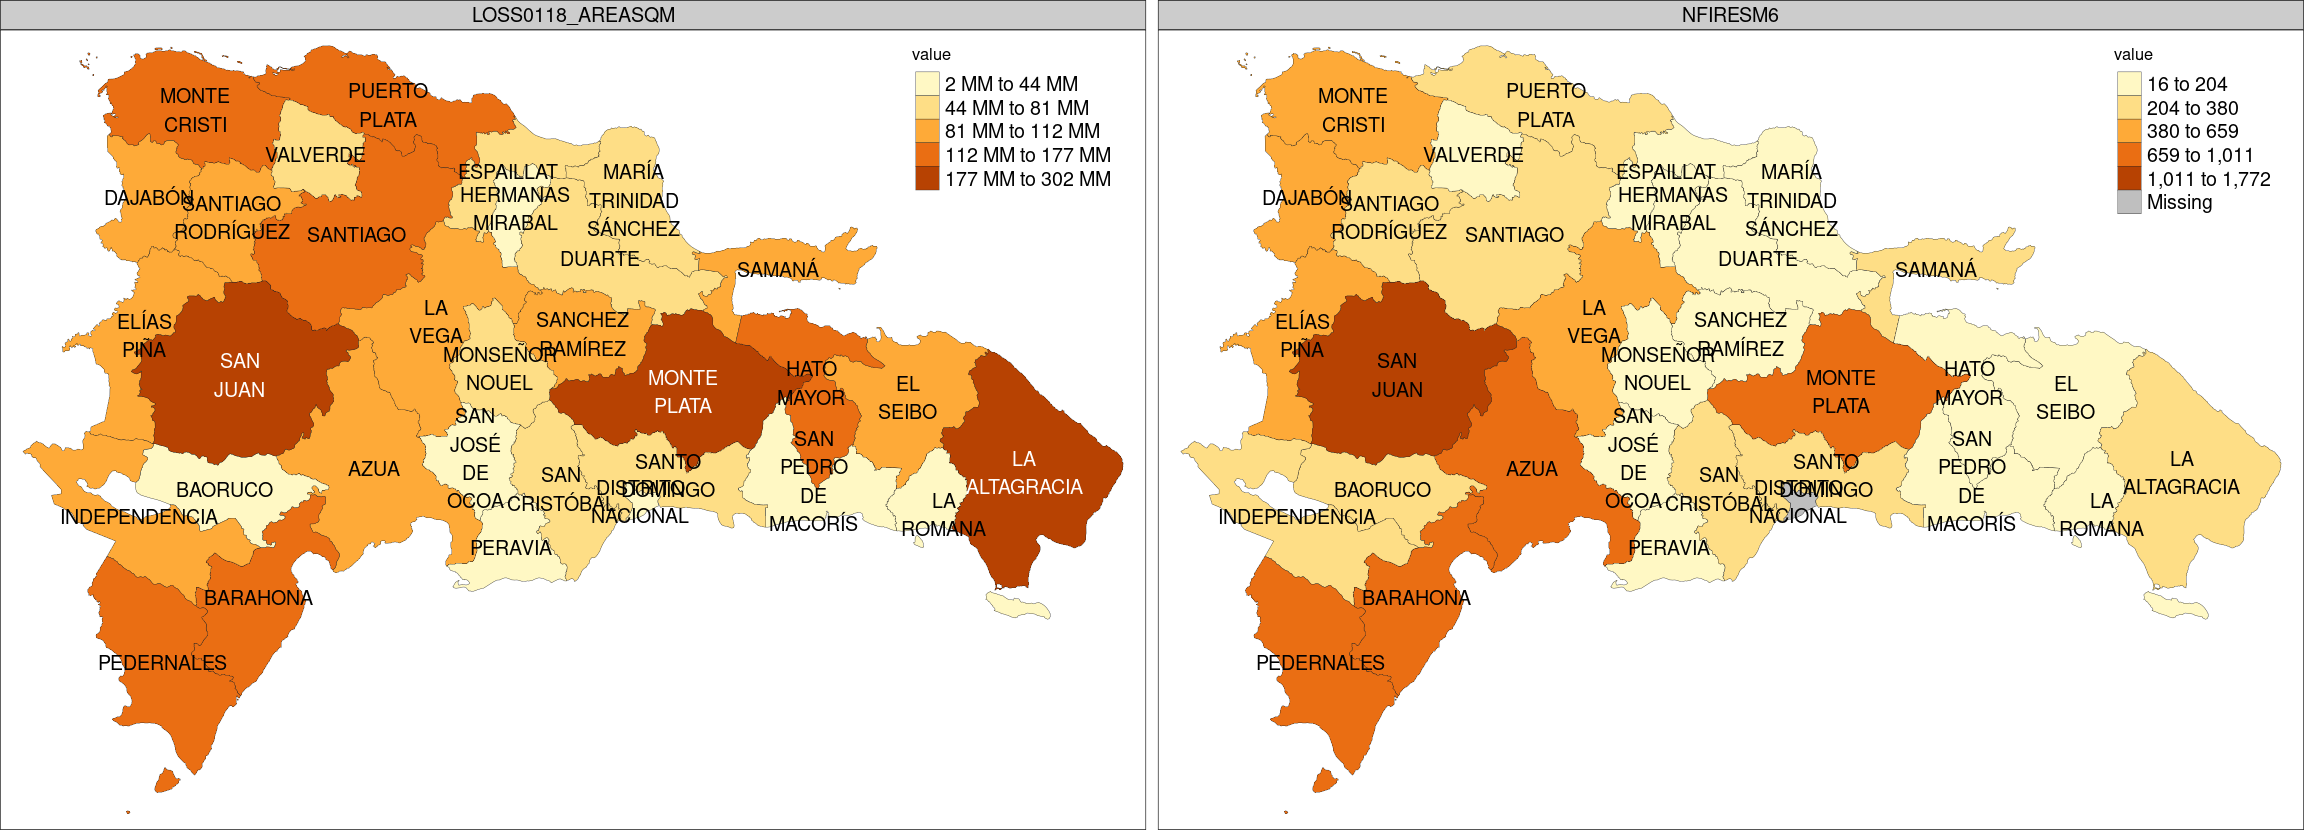
\includegraphics{img/data-download-preparation-eda/zonal-prov-7} \end{center}

\begin{Shaded}
\begin{Highlighting}[]
\CommentTok{\# Top twenty sorted descending by column 2}
\FunctionTok{stripped\_table}\NormalTok{(provzonal }\SpecialCharTok{\%\textgreater{}\%} \FunctionTok{select}\NormalTok{(}\FunctionTok{matches}\NormalTok{(}\StringTok{\textquotesingle{}\^{}LOSS0118\_AREASQM|NFIRESM6|TOPONIMIA\textquotesingle{}}\NormalTok{)) }\SpecialCharTok{\%\textgreater{}\%} \FunctionTok{select}\NormalTok{(}\SpecialCharTok{{-}}\FunctionTok{matches}\NormalTok{(}\StringTok{\textquotesingle{}\textless{}NA\textgreater{}\textquotesingle{}}\NormalTok{)))}
\end{Highlighting}
\end{Shaded}

\begin{table}[H]
\centering
\begin{tabular}[t]{llrr}
\toprule
  & TOPONIMIA & LOSS0118\_AREASQM & NFIRESM6\\
\midrule
\cellcolor{lightgray}{1} & \cellcolor{lightgray}{MONTE PLATA} & \cellcolor{lightgray}{302473946} & \cellcolor{lightgray}{791}\\
2 & LA ALTAGRACIA & 249292186 & 230\\
\cellcolor{lightgray}{3} & \cellcolor{lightgray}{SAN JUAN} & \cellcolor{lightgray}{220712371} & \cellcolor{lightgray}{1772}\\
4 & SANTIAGO & 176542269 & 380\\
\cellcolor{lightgray}{5} & \cellcolor{lightgray}{PUERTO PLATA} & \cellcolor{lightgray}{172314432} & \cellcolor{lightgray}{289}\\
\addlinespace
6 & PEDERNALES & 162766292 & 1011\\
\cellcolor{lightgray}{7} & \cellcolor{lightgray}{MONTE CRISTI} & \cellcolor{lightgray}{154799087} & \cellcolor{lightgray}{554}\\
8 & BARAHONA & 152451002 & 1006\\
\cellcolor{lightgray}{9} & \cellcolor{lightgray}{HATO MAYOR} & \cellcolor{lightgray}{140126481} & \cellcolor{lightgray}{193}\\
10 & SANCHEZ RAMÍREZ & 112409320 & 204\\
\addlinespace
\cellcolor{lightgray}{11} & \cellcolor{lightgray}{INDEPENDENCIA} & \cellcolor{lightgray}{108304461} & \cellcolor{lightgray}{363}\\
12 & LA VEGA & 108247674 & 475\\
\cellcolor{lightgray}{13} & \cellcolor{lightgray}{DAJABÓN} & \cellcolor{lightgray}{107101625} & \cellcolor{lightgray}{444}\\
14 & SANTIAGO RODRÍGUEZ & 102759738 & 349\\
\cellcolor{lightgray}{15} & \cellcolor{lightgray}{AZUA} & \cellcolor{lightgray}{97059365} & \cellcolor{lightgray}{908}\\
\addlinespace
16 & SAMANÁ & 96922649 & 248\\
\cellcolor{lightgray}{17} & \cellcolor{lightgray}{ELÍAS PIÑA} & \cellcolor{lightgray}{95820932} & \cellcolor{lightgray}{659}\\
18 & EL SEIBO & 89985798 & 75\\
\cellcolor{lightgray}{19} & \cellcolor{lightgray}{SAN CRISTÓBAL} & \cellcolor{lightgray}{81182825} & \cellcolor{lightgray}{226}\\
20 & SANTO DOMINGO & 78261478 & 258\\
\bottomrule
\end{tabular}
\end{table}

\begin{Shaded}
\begin{Highlighting}[]
\CommentTok{\# Fires V1}
\NormalTok{provzonal }\SpecialCharTok{\%\textgreater{}\%} \FunctionTok{select}\NormalTok{(}\FunctionTok{matches}\NormalTok{(}\StringTok{\textquotesingle{}\^{}LOSS1218|NFIRESV1\textquotesingle{}}\NormalTok{)) }\SpecialCharTok{\%\textgreater{}\%} \FunctionTok{select}\NormalTok{(}\SpecialCharTok{{-}}\FunctionTok{matches}\NormalTok{(}\StringTok{\textquotesingle{}\textless{}NA\textgreater{}\textquotesingle{}}\NormalTok{)) }\SpecialCharTok{\%\textgreater{}\%} 
  \FunctionTok{gather}\NormalTok{(variable, value, }\SpecialCharTok{{-}}\NormalTok{geom) }\SpecialCharTok{\%\textgreater{}\%}
  \FunctionTok{mutate}\NormalTok{(}\AttributeTok{variable =} \FunctionTok{factor}\NormalTok{(variable, }\AttributeTok{levels =} \FunctionTok{unique}\NormalTok{(variable))) }\SpecialCharTok{\%\textgreater{}\%} 
  \FunctionTok{tm\_shape}\NormalTok{() }\SpecialCharTok{+}
  \FunctionTok{tm\_fill}\NormalTok{(}\AttributeTok{col=}\StringTok{\textquotesingle{}value\textquotesingle{}}\NormalTok{, }\AttributeTok{palette =} \StringTok{"YlOrBr"}\NormalTok{, }\AttributeTok{size =} \FloatTok{0.1}\NormalTok{, }\AttributeTok{style =} \StringTok{\textquotesingle{}jenks\textquotesingle{}}\NormalTok{) }\SpecialCharTok{+}
  \FunctionTok{tm\_borders}\NormalTok{(}\AttributeTok{col =} \StringTok{\textquotesingle{}grey15\textquotesingle{}}\NormalTok{, }\AttributeTok{lwd =} \FloatTok{0.3}\NormalTok{) }\SpecialCharTok{+}
  \FunctionTok{tm\_facets}\NormalTok{(}\AttributeTok{by =} \StringTok{"variable"}\NormalTok{, }\AttributeTok{ncol =} \DecValTok{3}\NormalTok{, }\AttributeTok{nrow =} \DecValTok{1}\NormalTok{, }\AttributeTok{free.coords =} \ConstantTok{FALSE}\NormalTok{, }\AttributeTok{free.scales =} \ConstantTok{TRUE}\NormalTok{) }\SpecialCharTok{+}
  \FunctionTok{tm\_layout}\NormalTok{(}\AttributeTok{panel.label.size =} \DecValTok{1}\NormalTok{, }\AttributeTok{legend.title.size =} \DecValTok{1}\NormalTok{, }\AttributeTok{legend.text.size =} \DecValTok{1}\NormalTok{)}
\end{Highlighting}
\end{Shaded}

\begin{center}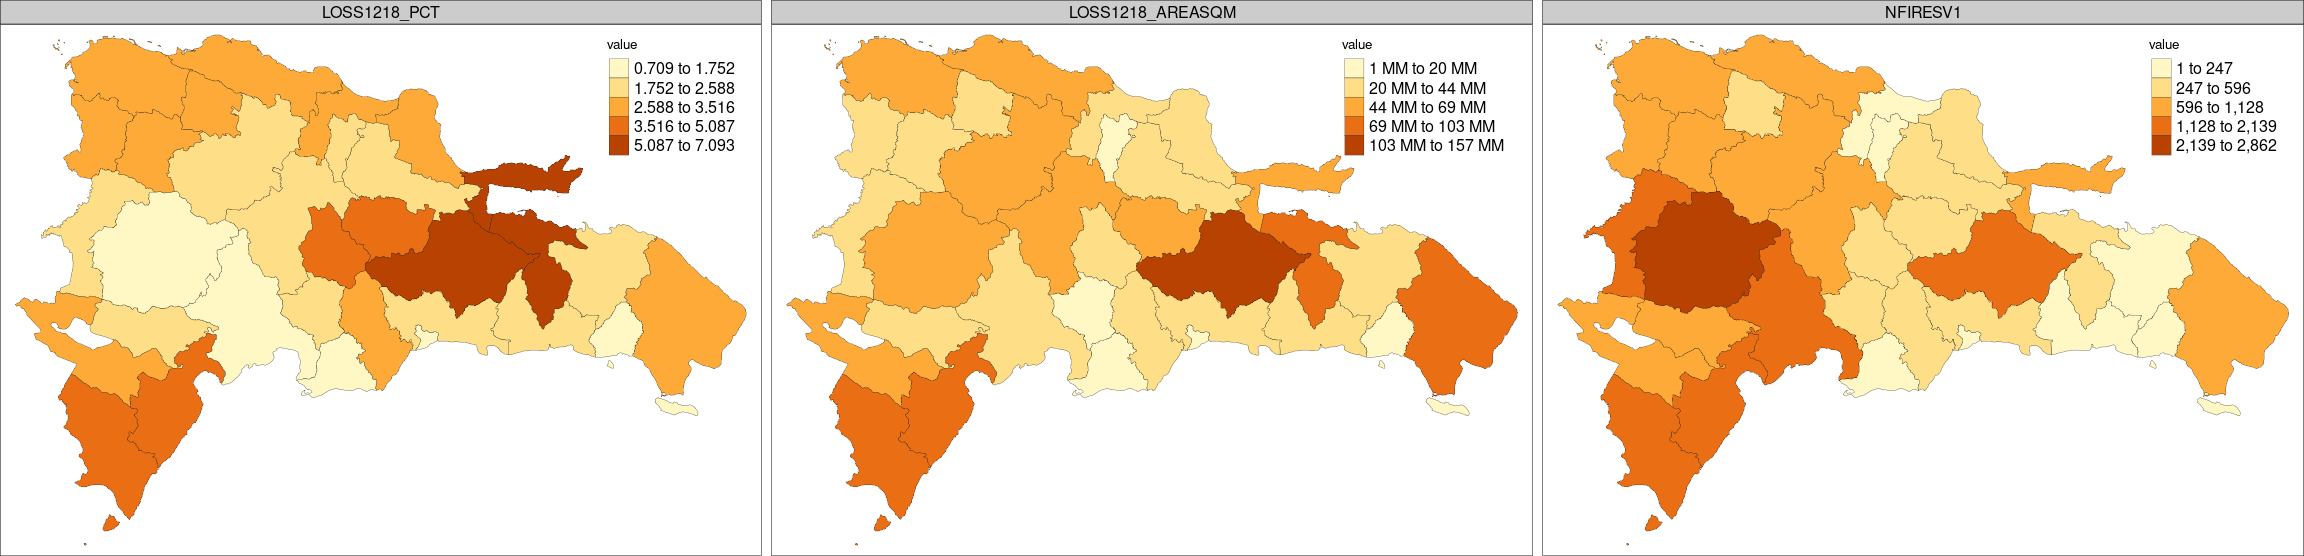
\includegraphics{img/data-download-preparation-eda/zonal-prov-8} \end{center}

\begin{Shaded}
\begin{Highlighting}[]
\CommentTok{\# Top twenty sorted descending by column 2}
\FunctionTok{stripped\_table}\NormalTok{(provzonal }\SpecialCharTok{\%\textgreater{}\%} \FunctionTok{select}\NormalTok{(TOPONIMIA, }\FunctionTok{matches}\NormalTok{(}\StringTok{\textquotesingle{}\^{}LOSS1218|NFIRESV1\textquotesingle{}}\NormalTok{)) }\SpecialCharTok{\%\textgreater{}\%} \FunctionTok{select}\NormalTok{(}\SpecialCharTok{{-}}\FunctionTok{matches}\NormalTok{(}\StringTok{\textquotesingle{}\textless{}NA\textgreater{}\textquotesingle{}}\NormalTok{)))}
\end{Highlighting}
\end{Shaded}

\begin{table}[H]
\centering
\begin{tabular}[t]{llrrr}
\toprule
  & TOPONIMIA & LOSS1218\_PCT & LOSS1218\_AREASQM & NFIRESV1\\
\midrule
\cellcolor{lightgray}{1} & \cellcolor{lightgray}{SAMANÁ} & \cellcolor{lightgray}{7.092585} & \cellcolor{lightgray}{61201256} & \cellcolor{lightgray}{835}\\
2 & HATO MAYOR & 6.610836 & 87102708 & 555\\
\cellcolor{lightgray}{3} & \cellcolor{lightgray}{MONTE PLATA} & \cellcolor{lightgray}{6.026899} & \cellcolor{lightgray}{156843601} & \cellcolor{lightgray}{1589}\\
4 & BARAHONA & 5.086634 & 84460081 & 2139\\
\cellcolor{lightgray}{5} & \cellcolor{lightgray}{PEDERNALES} & \cellcolor{lightgray}{4.685672} & \cellcolor{lightgray}{97464819} & \cellcolor{lightgray}{1894}\\
\addlinespace
6 & SANCHEZ RAMÍREZ & 4.543726 & 53874049 & 376\\
\cellcolor{lightgray}{7} & \cellcolor{lightgray}{MONSEÑOR NOUEL} & \cellcolor{lightgray}{4.053136} & \cellcolor{lightgray}{40206403} & \cellcolor{lightgray}{387}\\
8 & DAJABÓN & 3.516272 & 35892309 & 931\\
\cellcolor{lightgray}{9} & \cellcolor{lightgray}{PUERTO PLATA} & \cellcolor{lightgray}{3.508532} & \cellcolor{lightgray}{63368918} & \cellcolor{lightgray}{883}\\
10 & INDEPENDENCIA & 3.505947 & 62076489 & 897\\
\addlinespace
\cellcolor{lightgray}{11} & \cellcolor{lightgray}{LA ALTAGRACIA} & \cellcolor{lightgray}{3.432450} & \cellcolor{lightgray}{102838057} & \cellcolor{lightgray}{794}\\
12 & MARÍA TRINIDAD SÁNCHEZ & 3.342606 & 40327565 & 348\\
\cellcolor{lightgray}{13} & \cellcolor{lightgray}{ESPAILLAT} & \cellcolor{lightgray}{3.308128} & \cellcolor{lightgray}{27851494} & \cellcolor{lightgray}{187}\\
14 & SAN CRISTÓBAL & 3.174297 & 39385647 & 596\\
\cellcolor{lightgray}{15} & \cellcolor{lightgray}{VALVERDE} & \cellcolor{lightgray}{3.067846} & \cellcolor{lightgray}{25239085} & \cellcolor{lightgray}{390}\\
\addlinespace
16 & SANTIAGO RODRÍGUEZ & 3.007655 & 34532810 & 807\\
\cellcolor{lightgray}{17} & \cellcolor{lightgray}{MONTE CRISTI} & \cellcolor{lightgray}{2.931488} & \cellcolor{lightgray}{55185337} & \cellcolor{lightgray}{1123}\\
18 & ELÍAS PIÑA & 2.588126 & 36119894 & 1624\\
\cellcolor{lightgray}{19} & \cellcolor{lightgray}{SANTO DOMINGO} & \cellcolor{lightgray}{2.564897} & \cellcolor{lightgray}{33380362} & \cellcolor{lightgray}{502}\\
20 & LA VEGA & 2.475496 & 56754936 & 1128\\
\bottomrule
\end{tabular}
\end{table}

\hypertarget{zonal-by-municipalities}{%
\subsection{Zonal, by municipalities}\label{zonal-by-municipalities}}

\begin{Shaded}
\begin{Highlighting}[]
\CommentTok{\#Zonal statistics object}
\NormalTok{munzonal }\OtherTok{\textless{}{-}} \FunctionTok{readRDS}\NormalTok{(}\StringTok{\textquotesingle{}out/mun\_zonal\_statistics.RDS\textquotesingle{}}\NormalTok{)}

\CommentTok{\# Tree cover for pctc threshold}
\NormalTok{munzonal }\SpecialCharTok{\%\textgreater{}\%} \FunctionTok{select}\NormalTok{(}\FunctionTok{matches}\NormalTok{(}\StringTok{\textquotesingle{}\^{}TREECOVER2000\textquotesingle{}}\NormalTok{)) }\SpecialCharTok{\%\textgreater{}\%}
  \FunctionTok{gather}\NormalTok{(variable, value, }\SpecialCharTok{{-}}\NormalTok{geom) }\SpecialCharTok{\%\textgreater{}\%}
  \FunctionTok{tm\_shape}\NormalTok{() }\SpecialCharTok{+}
  \FunctionTok{tm\_fill}\NormalTok{(}\AttributeTok{col=}\StringTok{\textquotesingle{}value\textquotesingle{}}\NormalTok{, }\AttributeTok{palette =} \StringTok{"YlOrBr"}\NormalTok{, }\AttributeTok{size =} \FloatTok{0.1}\NormalTok{, }\AttributeTok{style =} \StringTok{\textquotesingle{}jenks\textquotesingle{}}\NormalTok{) }\SpecialCharTok{+}
  \FunctionTok{tm\_borders}\NormalTok{(}\AttributeTok{col =} \StringTok{\textquotesingle{}grey15\textquotesingle{}}\NormalTok{, }\AttributeTok{lwd =} \FloatTok{0.3}\NormalTok{) }\SpecialCharTok{+}
  \FunctionTok{tm\_facets}\NormalTok{(}\AttributeTok{by =} \StringTok{"variable"}\NormalTok{, }\AttributeTok{ncol =} \DecValTok{2}\NormalTok{, }\AttributeTok{nrow =} \DecValTok{2}\NormalTok{, }\AttributeTok{free.coords =} \ConstantTok{FALSE}\NormalTok{, }\AttributeTok{free.scales =} \ConstantTok{TRUE}\NormalTok{) }\SpecialCharTok{+}
  \FunctionTok{tm\_layout}\NormalTok{(}\AttributeTok{panel.label.size =} \DecValTok{1}\NormalTok{, }\AttributeTok{legend.title.size =} \DecValTok{1}\NormalTok{, }\AttributeTok{legend.text.size =} \DecValTok{1}\NormalTok{)}
\end{Highlighting}
\end{Shaded}

\begin{center}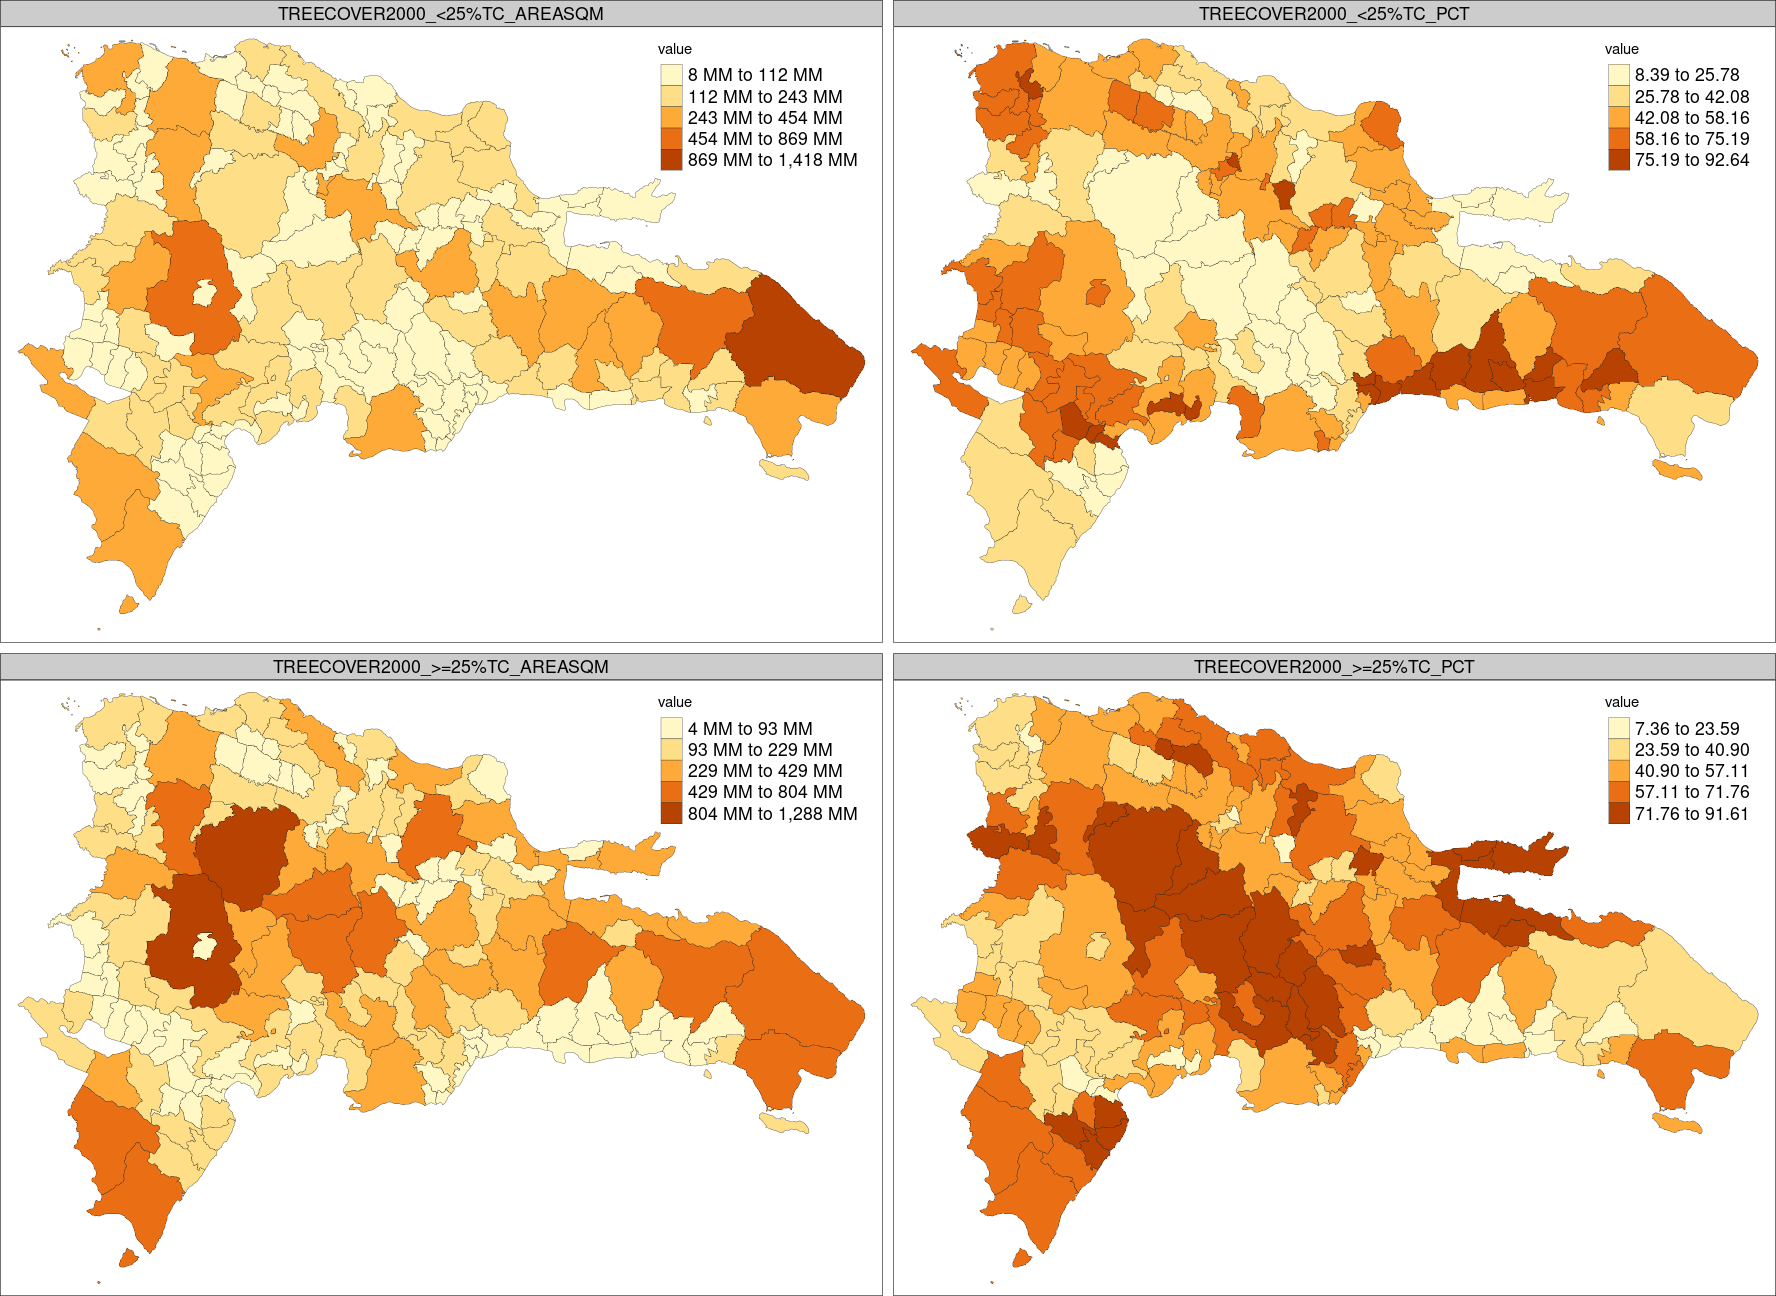
\includegraphics{img/data-download-preparation-eda/zonal-mun-1} \end{center}

\begin{Shaded}
\begin{Highlighting}[]
\CommentTok{\# Top twenty sorted descending by column 2}
\FunctionTok{stripped\_table}\NormalTok{(munzonal }\SpecialCharTok{\%\textgreater{}\%} \FunctionTok{select}\NormalTok{(TOPONIMIA, }\FunctionTok{matches}\NormalTok{(}\StringTok{\textquotesingle{}\^{}TREECOVER2000\textquotesingle{}}\NormalTok{)))}
\end{Highlighting}
\end{Shaded}

\begin{table}[H]
\centering
\begin{tabular}[t]{llrrrr}
\toprule
  & TOPONIMIA & TREECOVER2000\_>=25\%TC\_PCT & TREECOVER2000\_<25\%TC\_PCT & TREECOVER2000\_>=25\%TC\_AREASQM & TREECOVER2000\_<25\%TC\_AREASQM\\
\midrule
\cellcolor{lightgray}{1} & \cellcolor{lightgray}{LOS CACAOS} & \cellcolor{lightgray}{91.61025} & \cellcolor{lightgray}{8.389754} & \cellcolor{lightgray}{170310186} & \cellcolor{lightgray}{15597171}\\
2 & CAMBITA GARABITOS & 88.01608 & 11.983923 & 152082966 & 20707019\\
\cellcolor{lightgray}{3} & \cellcolor{lightgray}{GUANANICO} & \cellcolor{lightgray}{86.68482} & \cellcolor{lightgray}{13.315184} & \cellcolor{lightgray}{51772418} & \cellcolor{lightgray}{7952480}\\
4 & LA CIÉNAGA & 86.25875 & 13.741251 & 100812553 & 16059711\\
\cellcolor{lightgray}{5} & \cellcolor{lightgray}{SAN JOSÉ DE LAS MATAS} & \cellcolor{lightgray}{84.83461} & \cellcolor{lightgray}{15.165392} & \cellcolor{lightgray}{1288326327} & \cellcolor{lightgray}{230306637}\\
\addlinespace
6 & ALTAMIRA & 84.81078 & 15.189217 & 150498020 & 26953497\\
\cellcolor{lightgray}{7} & \cellcolor{lightgray}{JARABACOA} & \cellcolor{lightgray}{83.88671} & \cellcolor{lightgray}{16.113288} & \cellcolor{lightgray}{565469306} & \cellcolor{lightgray}{108617561}\\
8 & SABANA DE LA MAR & 83.82227 & 16.177732 & 428565345 & 82713285\\
\cellcolor{lightgray}{9} & \cellcolor{lightgray}{EL VALLE} & \cellcolor{lightgray}{81.81502} & \cellcolor{lightgray}{18.184984} & \cellcolor{lightgray}{133096980} & \cellcolor{lightgray}{29583401}\\
10 & MONCIÓN & 81.57768 & 18.422318 & 113607682 & 25655507\\
\addlinespace
\cellcolor{lightgray}{11} & \cellcolor{lightgray}{SAMANÁ} & \cellcolor{lightgray}{81.37407} & \cellcolor{lightgray}{18.625933} & \cellcolor{lightgray}{334161130} & \cellcolor{lightgray}{76487058}\\
12 & POLO & 81.24050 & 18.759498 & 167925531 & 38776208\\
\cellcolor{lightgray}{13} & \cellcolor{lightgray}{SÁNCHEZ} & \cellcolor{lightgray}{81.01879} & \cellcolor{lightgray}{18.981205} & \cellcolor{lightgray}{275912749} & \cellcolor{lightgray}{64641255}\\
14 & BONAO & 80.30119 & 19.698809 & 544425648 & 133553899\\
\cellcolor{lightgray}{15} & \cellcolor{lightgray}{CASTILLO} & \cellcolor{lightgray}{80.11398} & \cellcolor{lightgray}{19.886025} & \cellcolor{lightgray}{106634362} & \cellcolor{lightgray}{26468959}\\
\addlinespace
16 & RANCHO ARRIBA & 79.64393 & 20.356072 & 163233018 & 41720483\\
\cellcolor{lightgray}{17} & \cellcolor{lightgray}{PIEDRA BLANCA} & \cellcolor{lightgray}{79.41746} & \cellcolor{lightgray}{20.582538} & \cellcolor{lightgray}{183684957} & \cellcolor{lightgray}{47605432}\\
18 & CONSTANZA & 78.95450 & 21.045497 & 671456447 & 178978201\\
\cellcolor{lightgray}{19} & \cellcolor{lightgray}{VILLA ALTAGRACIA} & \cellcolor{lightgray}{78.83552} & \cellcolor{lightgray}{21.164480} & \cellcolor{lightgray}{336034321} & \cellcolor{lightgray}{90213039}\\
20 & PARAÍSO & 78.76318 & 21.236825 & 107250173 & 28917742\\
\bottomrule
\end{tabular}
\end{table}

\begin{Shaded}
\begin{Highlighting}[]

\CommentTok{\# Loss year}
\CommentTok{\# * PCT}
\NormalTok{munzonal }\SpecialCharTok{\%\textgreater{}\%} \FunctionTok{select}\NormalTok{(}\FunctionTok{matches}\NormalTok{(}\StringTok{\textquotesingle{}\^{}LOSSYEAR\_[1{-}9].*\_PCT$\textquotesingle{}}\NormalTok{)) }\SpecialCharTok{\%\textgreater{}\%}
  \FunctionTok{gather}\NormalTok{(variable, value, }\SpecialCharTok{{-}}\NormalTok{geom) }\SpecialCharTok{\%\textgreater{}\%}
  \FunctionTok{mutate}\NormalTok{(}\AttributeTok{variable =} \FunctionTok{factor}\NormalTok{(variable, }\AttributeTok{levels =} \FunctionTok{unique}\NormalTok{(variable))) }\SpecialCharTok{\%\textgreater{}\%} 
  \FunctionTok{tm\_shape}\NormalTok{() }\SpecialCharTok{+}
  \FunctionTok{tm\_fill}\NormalTok{(}\AttributeTok{col=}\StringTok{\textquotesingle{}value\textquotesingle{}}\NormalTok{, }\AttributeTok{palette =} \StringTok{"YlOrBr"}\NormalTok{, }\AttributeTok{size =} \FloatTok{0.1}\NormalTok{, }\AttributeTok{style =} \StringTok{\textquotesingle{}jenks\textquotesingle{}}\NormalTok{) }\SpecialCharTok{+}
  \FunctionTok{tm\_borders}\NormalTok{(}\AttributeTok{col =} \StringTok{\textquotesingle{}grey15\textquotesingle{}}\NormalTok{, }\AttributeTok{lwd =} \FloatTok{0.3}\NormalTok{) }\SpecialCharTok{+}
  \FunctionTok{tm\_facets}\NormalTok{(}\AttributeTok{by =} \StringTok{"variable"}\NormalTok{, }\AttributeTok{ncol =} \DecValTok{5}\NormalTok{, }\AttributeTok{nrow =} \DecValTok{4}\NormalTok{, }\AttributeTok{free.coords =} \ConstantTok{FALSE}\NormalTok{, }\AttributeTok{free.scales =} \ConstantTok{TRUE}\NormalTok{) }\SpecialCharTok{+}
  \FunctionTok{tm\_layout}\NormalTok{(}\AttributeTok{panel.label.size =} \DecValTok{1}\NormalTok{, }\AttributeTok{legend.title.size =} \DecValTok{1}\NormalTok{, }\AttributeTok{legend.text.size =} \FloatTok{0.75}\NormalTok{)}
\end{Highlighting}
\end{Shaded}

\begin{center}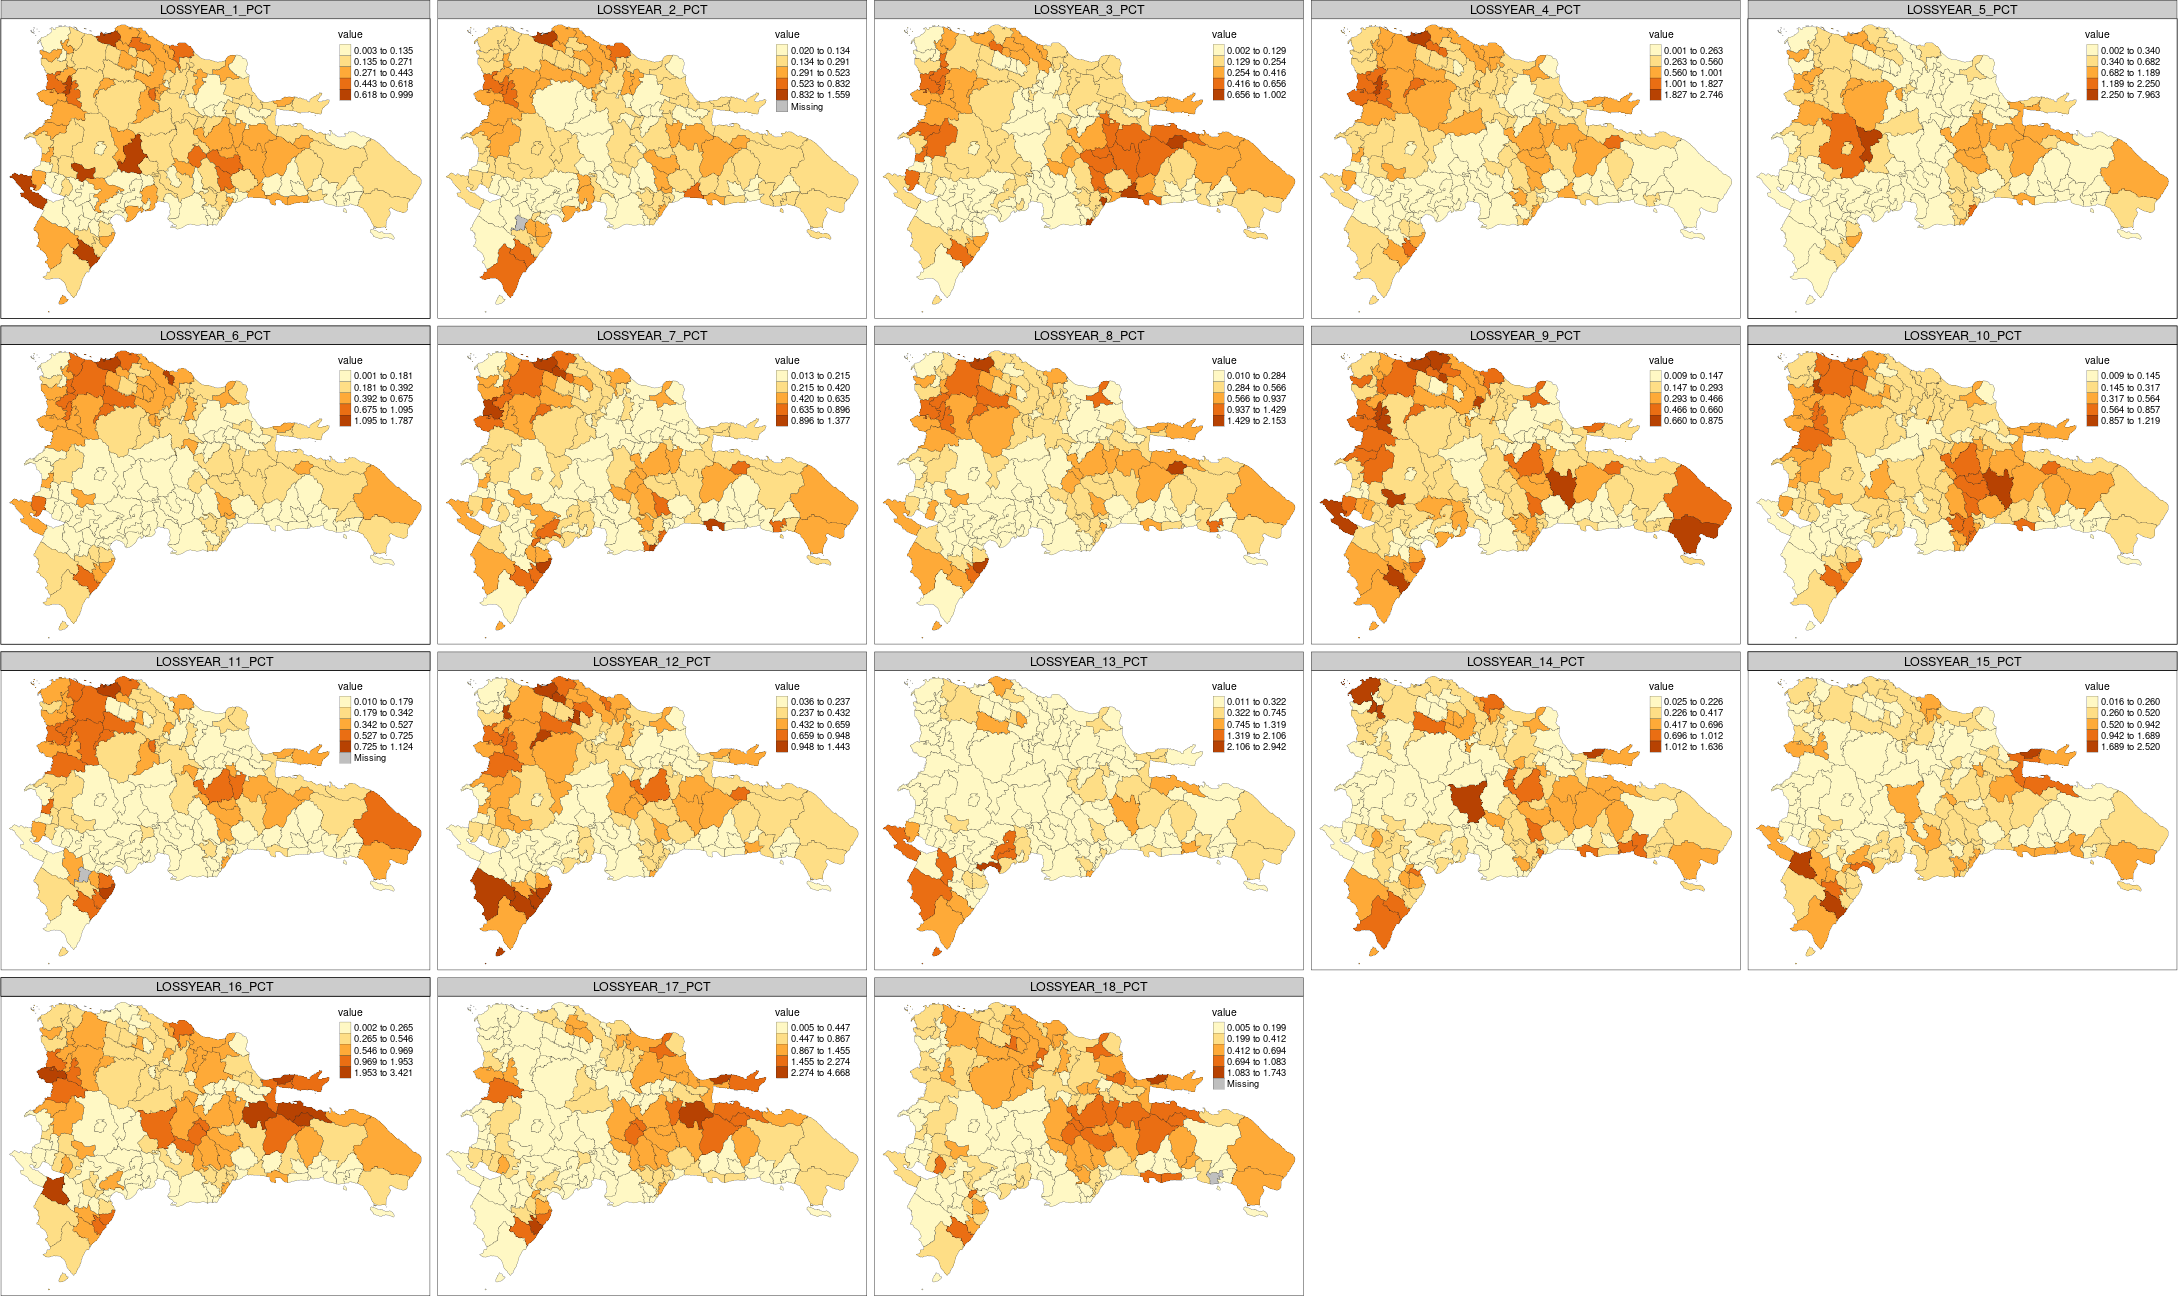
\includegraphics{img/data-download-preparation-eda/zonal-mun-2} \end{center}

\begin{Shaded}
\begin{Highlighting}[]
\CommentTok{\# Top twenty sorted descending by column 2}
\FunctionTok{stripped\_table}\NormalTok{(munzonal }\SpecialCharTok{\%\textgreater{}\%} \FunctionTok{select}\NormalTok{(TOPONIMIA, }\FunctionTok{matches}\NormalTok{(}\StringTok{\textquotesingle{}\^{}LOSSYEAR\_[1{-}9].*\_PCT$\textquotesingle{}}\NormalTok{)))}
\end{Highlighting}
\end{Shaded}

\begin{table}[H]
\centering
\resizebox{\linewidth}{!}{
\begin{tabular}[t]{llrrrrrrrrrrrrrrrrrr}
\toprule
  & TOPONIMIA & LOSSYEAR\_1\_PCT & LOSSYEAR\_2\_PCT & LOSSYEAR\_3\_PCT & LOSSYEAR\_4\_PCT & LOSSYEAR\_5\_PCT & LOSSYEAR\_6\_PCT & LOSSYEAR\_7\_PCT & LOSSYEAR\_8\_PCT & LOSSYEAR\_9\_PCT & LOSSYEAR\_10\_PCT & LOSSYEAR\_11\_PCT & LOSSYEAR\_12\_PCT & LOSSYEAR\_13\_PCT & LOSSYEAR\_14\_PCT & LOSSYEAR\_15\_PCT & LOSSYEAR\_16\_PCT & LOSSYEAR\_17\_PCT & LOSSYEAR\_18\_PCT\\
\midrule
\cellcolor{lightgray}{1} & \cellcolor{lightgray}{VILLA ISABELA} & \cellcolor{lightgray}{0.9994303} & \cellcolor{lightgray}{1.5587222} & \cellcolor{lightgray}{0.3272379} & \cellcolor{lightgray}{2.7457410} & \cellcolor{lightgray}{0.9591335} & \cellcolor{lightgray}{1.7873023} & \cellcolor{lightgray}{0.9785871} & \cellcolor{lightgray}{1.7650696} & \cellcolor{lightgray}{0.7962093} & \cellcolor{lightgray}{0.6961621} & \cellcolor{lightgray}{1.0209682} & \cellcolor{lightgray}{1.4430425} & \cellcolor{lightgray}{0.2285802} & \cellcolor{lightgray}{0.2813829} & \cellcolor{lightgray}{0.4140844} & \cellcolor{lightgray}{0.2567185} & \cellcolor{lightgray}{0.5169108} & \cellcolor{lightgray}{0.2938888}\\
2 & ENRIQUILLO & 0.9741060 & 0.6360274 & 0.6564287 & 0.6322161 & 0.5140679 & 0.9698464 & 0.8297276 & 0.9187311 & 0.8747898 & 0.8351082 & 0.6281807 & 1.3886336 & 1.0225311 & 0.8126892 & 2.5122744 & 0.8505773 & 2.2737361 & 0.8274857\\
\cellcolor{lightgray}{3} & \cellcolor{lightgray}{PADRE LAS CASAS} & \cellcolor{lightgray}{0.7909467} & \cellcolor{lightgray}{0.2051742} & \cellcolor{lightgray}{0.1373385} & \cellcolor{lightgray}{0.2603148} & \cellcolor{lightgray}{0.6518129} & \cellcolor{lightgray}{0.0943801} & \cellcolor{lightgray}{0.1906838} & \cellcolor{lightgray}{0.2786523} & \cellcolor{lightgray}{0.1831180} & \cellcolor{lightgray}{0.3991921} & \cellcolor{lightgray}{0.1084859} & \cellcolor{lightgray}{0.1606771} & \cellcolor{lightgray}{0.0784791} & \cellcolor{lightgray}{0.1559324} & \cellcolor{lightgray}{0.0732216} & \cellcolor{lightgray}{0.2397974} & \cellcolor{lightgray}{0.2336422} & \cellcolor{lightgray}{0.1301574}\\
4 & JIMANÍ & 0.7506408 & 0.2061926 & 0.2002747 & 0.3275099 & 0.2027665 & 0.5861851 & 0.5534808 & 0.6794701 & 0.6883470 & 0.1169567 & 0.1164895 & 0.2161596 & 1.8974706 & 0.1579149 & 0.6850766 & 0.1737998 & 0.3672222 & 0.2677078\\
\cellcolor{lightgray}{5} & \cellcolor{lightgray}{EL PINO} & \cellcolor{lightgray}{0.7186764} & \cellcolor{lightgray}{0.7379641} & \cellcolor{lightgray}{0.4729679} & \cellcolor{lightgray}{2.3866429} & \cellcolor{lightgray}{0.6272694} & \cellcolor{lightgray}{0.8780095} & \cellcolor{lightgray}{0.6046274} & \cellcolor{lightgray}{1.2905985} & \cellcolor{lightgray}{0.7295781} & \cellcolor{lightgray}{0.6130133} & \cellcolor{lightgray}{0.5744379} & \cellcolor{lightgray}{0.7144834} & \cellcolor{lightgray}{0.0654105} & \cellcolor{lightgray}{0.0687648} & \cellcolor{lightgray}{0.1601717} & \cellcolor{lightgray}{0.5702450} & \cellcolor{lightgray}{0.4025258} & \cellcolor{lightgray}{0.1635261}\\
\addlinespace
6 & VALLEJUELO & 0.7154490 & 0.2195768 & 0.1807694 & 0.7167757 & 0.4719907 & 0.4437973 & 0.5608828 & 0.8033461 & 0.8577427 & 0.3247216 & 0.2033242 & 0.4889067 & 0.4305298 & 0.3253850 & 0.3356673 & 0.8640448 & 0.3466130 & 0.4341784\\
\cellcolor{lightgray}{7} & \cellcolor{lightgray}{SABANA IGLESIA} & \cellcolor{lightgray}{0.6179326} & \cellcolor{lightgray}{0.0800560} & \cellcolor{lightgray}{0.0037526} & \cellcolor{lightgray}{0.2864505} & \cellcolor{lightgray}{1.0469829} & \cellcolor{lightgray}{0.5691484} & \cellcolor{lightgray}{0.1826278} & \cellcolor{lightgray}{0.5178625} & \cellcolor{lightgray}{0.2289102} & \cellcolor{lightgray}{0.1350946} & \cellcolor{lightgray}{0.6967377} & \cellcolor{lightgray}{0.3877714} & \cellcolor{lightgray}{0.2126489} & \cellcolor{lightgray}{0.1751226} & \cellcolor{lightgray}{0.0738017} & \cellcolor{lightgray}{0.2326629} & \cellcolor{lightgray}{0.1601121} & \cellcolor{lightgray}{0.5829080}\\
8 & VILLA LOS ALMÁCIGOS & 0.6153966 & 0.5817006 & 0.4160578 & 1.3347190 & 0.5469404 & 0.5448122 & 0.6122044 & 1.0218776 & 0.7423776 & 0.6707291 & 0.4564931 & 0.9328491 & 0.2933331 & 0.2564448 & 0.6827888 & 1.2985401 & 0.9651263 & 0.5178554\\
\cellcolor{lightgray}{9} & \cellcolor{lightgray}{IMBERT} & \cellcolor{lightgray}{0.5791735} & \cellcolor{lightgray}{0.2706162} & \cellcolor{lightgray}{0.3579265} & \cellcolor{lightgray}{0.5074054} & \cellcolor{lightgray}{0.5869446} & \cellcolor{lightgray}{0.3085573} & \cellcolor{lightgray}{0.2962150} & \cellcolor{lightgray}{0.2825014} & \cellcolor{lightgray}{0.5810020} & \cellcolor{lightgray}{0.1220516} & \cellcolor{lightgray}{0.2980435} & \cellcolor{lightgray}{0.4356372} & \cellcolor{lightgray}{0.4552935} & \cellcolor{lightgray}{0.1572500} & \cellcolor{lightgray}{0.2751874} & \cellcolor{lightgray}{0.1993052} & \cellcolor{lightgray}{1.1652039} & \cellcolor{lightgray}{0.5668312}\\
10 & YAMASÁ & 0.5714324 & 0.4617893 & 0.5136452 & 0.6785337 & 0.7605542 & 0.2899528 & 0.3712955 & 0.5080529 & 0.3624834 & 0.8571487 & 0.3902755 & 0.3824801 & 0.2641943 & 0.6415905 & 0.2760568 & 0.6668406 & 1.4157019 & 0.7641130\\
\addlinespace
\cellcolor{lightgray}{11} & \cellcolor{lightgray}{PEDRO BRAND} & \cellcolor{lightgray}{0.5579235} & \cellcolor{lightgray}{0.4431545} & \cellcolor{lightgray}{0.6362053} & \cellcolor{lightgray}{0.9287669} & \cellcolor{lightgray}{0.6282445} & \cellcolor{lightgray}{0.6192885} & \cellcolor{lightgray}{0.8305830} & \cellcolor{lightgray}{0.6113276} & \cellcolor{lightgray}{0.5592504} & \cellcolor{lightgray}{0.7741935} & \cellcolor{lightgray}{0.3509412} & \cellcolor{lightgray}{0.4769881} & \cellcolor{lightgray}{0.6073472} & \cellcolor{lightgray}{0.7798325} & \cellcolor{lightgray}{0.4560909} & \cellcolor{lightgray}{0.6279128} & \cellcolor{lightgray}{0.9360644} & \cellcolor{lightgray}{0.6892777}\\
12 & LOMA DE CABRERA & 0.5183806 & 0.8317367 & 0.4897309 & 1.8267170 & 0.7105723 & 0.6750586 & 0.9466340 & 1.2996819 & 0.6046281 & 0.4828669 & 0.5512084 & 0.7445939 & 0.2581458 & 0.2572505 & 0.3491683 & 1.5339529 & 0.8627739 & 0.3351418\\
\cellcolor{lightgray}{13} & \cellcolor{lightgray}{PIEDRA BLANCA} & \cellcolor{lightgray}{0.4968462} & \cellcolor{lightgray}{0.1663576} & \cellcolor{lightgray}{0.3253993} & \cellcolor{lightgray}{0.4141445} & \cellcolor{lightgray}{0.3352599} & \cellcolor{lightgray}{0.2710070} & \cellcolor{lightgray}{0.5391513} & \cellcolor{lightgray}{0.6794261} & \cellcolor{lightgray}{0.2121616} & \cellcolor{lightgray}{0.2407891} & \cellcolor{lightgray}{0.1669938} & \cellcolor{lightgray}{0.4895303} & \cellcolor{lightgray}{0.1526800} & \cellcolor{lightgray}{0.3918787} & \cellcolor{lightgray}{0.4768070} & \cellcolor{lightgray}{1.5652882} & \cellcolor{lightgray}{1.7755413} & \cellcolor{lightgray}{1.0477666}\\
14 & SOSÚA & 0.4791335 & 0.6287596 & 0.1823568 & 0.7544565 & 0.6568144 & 0.6034552 & 0.4791335 & 0.7038476 & 0.5322177 & 0.1911583 & 0.4466778 & 0.6026300 & 0.2956765 & 0.7585822 & 0.8994067 & 1.4065951 & 0.7841616 & 0.5985043\\
\cellcolor{lightgray}{15} & \cellcolor{lightgray}{VILLA MONTELLANO} & \cellcolor{lightgray}{0.4434884} & \cellcolor{lightgray}{0.4363518} & \cellcolor{lightgray}{0.2609955} & \cellcolor{lightgray}{0.6249618} & \cellcolor{lightgray}{0.1559856} & \cellcolor{lightgray}{1.2927431} & \cellcolor{lightgray}{0.3965907} & \cellcolor{lightgray}{0.4434884} & \cellcolor{lightgray}{0.3863956} & \cellcolor{lightgray}{0.2518198} & \cellcolor{lightgray}{0.1651612} & \cellcolor{lightgray}{0.8145913} & \cellcolor{lightgray}{0.1631222} & \cellcolor{lightgray}{0.5250494} & \cellcolor{lightgray}{0.4098444} & \cellcolor{lightgray}{0.8512938} & \cellcolor{lightgray}{0.4343127} & \cellcolor{lightgray}{0.2293905}\\
\addlinespace
16 & PARTIDO & 0.4430429 & 0.4793902 & 0.4710401 & 1.5712798 & 0.7804825 & 0.8649652 & 0.7524854 & 1.4288381 & 0.3182836 & 0.4425518 & 0.7023852 & 0.5761523 & 0.2401863 & 0.2667099 & 0.1458800 & 0.8227239 & 0.3870486 & 0.1552124\\
\cellcolor{lightgray}{17} & \cellcolor{lightgray}{BOHECHÍO} & \cellcolor{lightgray}{0.4351024} & \cellcolor{lightgray}{0.1731715} & \cellcolor{lightgray}{0.2097621} & \cellcolor{lightgray}{0.4023157} & \cellcolor{lightgray}{7.9629891} & \cellcolor{lightgray}{0.1181044} & \cellcolor{lightgray}{0.2718937} & \cellcolor{lightgray}{0.5387154} & \cellcolor{lightgray}{0.2539607} & \cellcolor{lightgray}{0.1228141} & \cellcolor{lightgray}{0.1693675} & \cellcolor{lightgray}{0.6142515} & \cellcolor{lightgray}{0.0547048} & \cellcolor{lightgray}{0.0599579} & \cellcolor{lightgray}{0.0157593} & \cellcolor{lightgray}{0.1889308} & \cellcolor{lightgray}{0.2244346} & \cellcolor{lightgray}{0.1488985}\\
18 & SABANA GRANDE DE BOYÁ & 0.4211248 & 0.4202882 & 0.6021249 & 0.6259700 & 1.0677328 & 0.3778968 & 0.4159654 & 0.6471657 & 0.2468182 & 0.4095509 & 0.4414839 & 0.5523429 & 0.5682397 & 0.6958321 & 0.5785586 & 2.2361451 & 3.0361428 & 0.9766750\\
\cellcolor{lightgray}{19} & \cellcolor{lightgray}{ESPERANZA} & \cellcolor{lightgray}{0.4145645} & \cellcolor{lightgray}{0.1649628} & \cellcolor{lightgray}{0.0564259} & \cellcolor{lightgray}{0.4112454} & \cellcolor{lightgray}{0.1052177} & \cellcolor{lightgray}{0.3066914} & \cellcolor{lightgray}{0.2346654} & \cellcolor{lightgray}{0.3773898} & \cellcolor{lightgray}{0.1301115} & \cellcolor{lightgray}{0.1530138} & \cellcolor{lightgray}{0.1387414} & \cellcolor{lightgray}{0.4089219} & \cellcolor{lightgray}{0.1390733} & \cellcolor{lightgray}{0.1925119} & \cellcolor{lightgray}{0.2127589} & \cellcolor{lightgray}{0.3053638} & \cellcolor{lightgray}{0.3013808} & \cellcolor{lightgray}{0.3123340}\\
20 & BAYAGUANA & 0.4138005 & 0.3508456 & 0.5494867 & 0.6481751 & 0.9717992 & 0.3920571 & 0.4871216 & 0.7446724 & 0.3075271 & 0.5049884 & 0.4105137 & 0.5175456 & 0.5072638 & 0.6392418 & 0.3631500 & 1.9532903 & 1.8679176 & 1.0832978\\
\bottomrule
\end{tabular}}
\end{table}

\begin{Shaded}
\begin{Highlighting}[]
\CommentTok{\# * AREASQM}
\NormalTok{munzonal }\SpecialCharTok{\%\textgreater{}\%} \FunctionTok{select}\NormalTok{(}\FunctionTok{matches}\NormalTok{(}\StringTok{\textquotesingle{}\^{}LOSSYEAR\_[1{-}9].*\_AREASQM$\textquotesingle{}}\NormalTok{)) }\SpecialCharTok{\%\textgreater{}\%}
  \FunctionTok{gather}\NormalTok{(variable, value, }\SpecialCharTok{{-}}\NormalTok{geom) }\SpecialCharTok{\%\textgreater{}\%}
  \FunctionTok{mutate}\NormalTok{(}\AttributeTok{variable =} \FunctionTok{factor}\NormalTok{(variable, }\AttributeTok{levels =} \FunctionTok{unique}\NormalTok{(variable))) }\SpecialCharTok{\%\textgreater{}\%} 
  \FunctionTok{tm\_shape}\NormalTok{() }\SpecialCharTok{+}
  \FunctionTok{tm\_fill}\NormalTok{(}\AttributeTok{col=}\StringTok{\textquotesingle{}value\textquotesingle{}}\NormalTok{, }\AttributeTok{palette =} \StringTok{"YlOrBr"}\NormalTok{, }\AttributeTok{size =} \FloatTok{0.1}\NormalTok{, }\AttributeTok{style =} \StringTok{\textquotesingle{}jenks\textquotesingle{}}\NormalTok{) }\SpecialCharTok{+}
  \FunctionTok{tm\_borders}\NormalTok{(}\AttributeTok{col =} \StringTok{\textquotesingle{}grey15\textquotesingle{}}\NormalTok{, }\AttributeTok{lwd =} \FloatTok{0.3}\NormalTok{) }\SpecialCharTok{+}
  \FunctionTok{tm\_facets}\NormalTok{(}\AttributeTok{by =} \StringTok{"variable"}\NormalTok{, }\AttributeTok{ncol =} \DecValTok{5}\NormalTok{, }\AttributeTok{nrow =} \DecValTok{4}\NormalTok{, }\AttributeTok{free.coords =} \ConstantTok{FALSE}\NormalTok{, }\AttributeTok{free.scales =} \ConstantTok{TRUE}\NormalTok{) }\SpecialCharTok{+}
  \FunctionTok{tm\_layout}\NormalTok{(}\AttributeTok{panel.label.size =} \DecValTok{1}\NormalTok{, }\AttributeTok{legend.title.size =} \DecValTok{1}\NormalTok{, }\AttributeTok{legend.text.size =} \FloatTok{0.75}\NormalTok{)}
\end{Highlighting}
\end{Shaded}

\begin{center}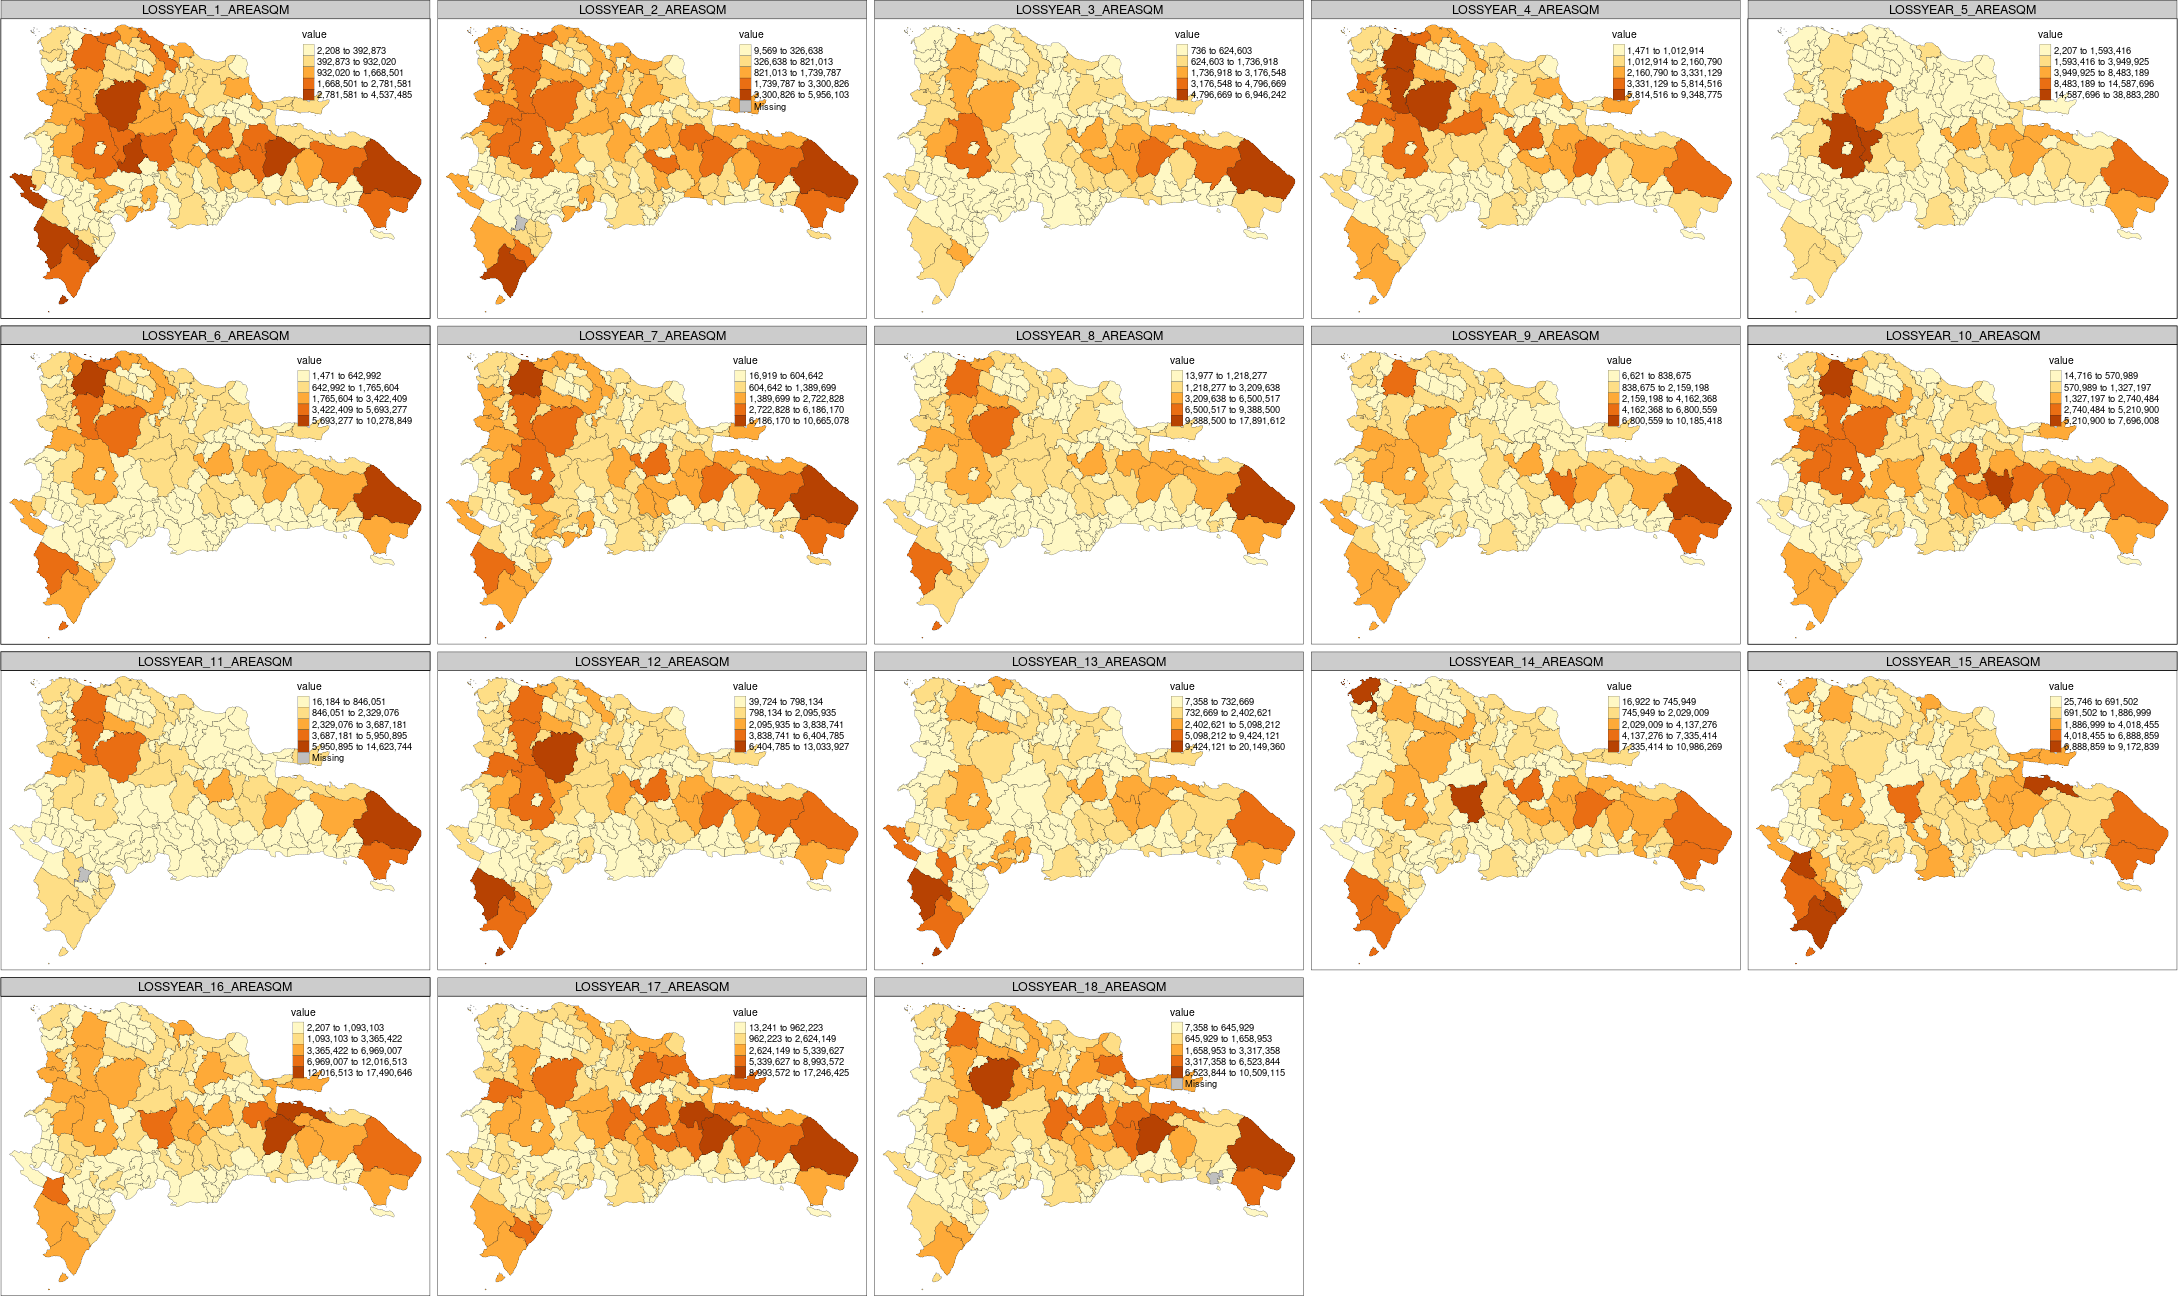
\includegraphics{img/data-download-preparation-eda/zonal-mun-3} \end{center}

\begin{Shaded}
\begin{Highlighting}[]
\CommentTok{\# Top twenty sorted descending by column 2}
\FunctionTok{stripped\_table}\NormalTok{(munzonal }\SpecialCharTok{\%\textgreater{}\%} \FunctionTok{select}\NormalTok{(TOPONIMIA, }\FunctionTok{matches}\NormalTok{(}\StringTok{\textquotesingle{}\^{}LOSSYEAR\_[1{-}9].*\_AREASQM$\textquotesingle{}}\NormalTok{)))}
\end{Highlighting}
\end{Shaded}

\begin{table}[H]
\centering
\resizebox{\linewidth}{!}{
\begin{tabular}[t]{llrrrrrrrrrrrrrrrrrr}
\toprule
  & TOPONIMIA & LOSSYEAR\_1\_AREASQM & LOSSYEAR\_2\_AREASQM & LOSSYEAR\_3\_AREASQM & LOSSYEAR\_4\_AREASQM & LOSSYEAR\_5\_AREASQM & LOSSYEAR\_6\_AREASQM & LOSSYEAR\_7\_AREASQM & LOSSYEAR\_8\_AREASQM & LOSSYEAR\_9\_AREASQM & LOSSYEAR\_10\_AREASQM & LOSSYEAR\_11\_AREASQM & LOSSYEAR\_12\_AREASQM & LOSSYEAR\_13\_AREASQM & LOSSYEAR\_14\_AREASQM & LOSSYEAR\_15\_AREASQM & LOSSYEAR\_16\_AREASQM & LOSSYEAR\_17\_AREASQM & LOSSYEAR\_18\_AREASQM\\
\midrule
\cellcolor{lightgray}{1} & \cellcolor{lightgray}{PADRE LAS CASAS} & \cellcolor{lightgray}{4537485} & \cellcolor{lightgray}{1177039.0} & \cellcolor{lightgray}{787880.5} & \cellcolor{lightgray}{1493368} & \cellcolor{lightgray}{3739305.7} & \cellcolor{lightgray}{541437.9} & \cellcolor{lightgray}{1093911} & \cellcolor{lightgray}{1598566} & \cellcolor{lightgray}{1050507} & \cellcolor{lightgray}{2290076.5} & \cellcolor{lightgray}{622359.4} & \cellcolor{lightgray}{921768.7} & \cellcolor{lightgray}{450217.4} & \cellcolor{lightgray}{894549.6} & \cellcolor{lightgray}{420055.79} & \cellcolor{lightgray}{1375664.3} & \cellcolor{lightgray}{1340353.1} & \cellcolor{lightgray}{746684.1}\\
2 & HIGÜEY & 4275742 & 5519768.2 & 6946241.7 & 4942263 & 14587696.1 & 10278848.7 & 10665078 & 17891612 & 10185418 & 4795864.2 & 14623744.2 & 6404785.0 & 7417809.3 & 7335413.7 & 6888859.08 & 12016512.6 & 17246425.0 & 10509114.9\\
\cellcolor{lightgray}{3} & \cellcolor{lightgray}{BAYAGUANA} & \cellcolor{lightgray}{3612216} & \cellcolor{lightgray}{3062658.6} & \cellcolor{lightgray}{4796669.3} & \cellcolor{lightgray}{5658157} & \cellcolor{lightgray}{8483189.3} & \cellcolor{lightgray}{3422408.8} & \cellcolor{lightgray}{4252262} & \cellcolor{lightgray}{6500517} & \cellcolor{lightgray}{2684516} & \cellcolor{lightgray}{4408227.4} & \cellcolor{lightgray}{3583524.0} & \cellcolor{lightgray}{4517844.5} & \cellcolor{lightgray}{4428090.9} & \cellcolor{lightgray}{5580174.4} & \cellcolor{lightgray}{3170068.73} & \cellcolor{lightgray}{17050982.3} & \cellcolor{lightgray}{16305733.0} & \cellcolor{lightgray}{9456501.1}\\
4 & JIMANÍ & 3545830 & 973999.8 & 946045.2 & 1547071 & 957815.6 & 2768984.4 & 2614498 & 3209638 & 3251570 & 552472.7 & 550265.8 & 1021081.4 & 8963152.6 & 745948.5 & 3236121.83 & 820984.8 & 1734661.4 & 1264581.4\\
\cellcolor{lightgray}{5} & \cellcolor{lightgray}{PEDERNALES} & \cellcolor{lightgray}{3208272} & \cellcolor{lightgray}{988745.1} & \cellcolor{lightgray}{1530200.8} & \cellcolor{lightgray}{3331129} & \cellcolor{lightgray}{3038331.4} & \cellcolor{lightgray}{3838008.4} & \cellcolor{lightgray}{5890537} & \cellcolor{lightgray}{8742743} & \cellcolor{lightgray}{3671011} & \cellcolor{lightgray}{1628045.4} & \cellcolor{lightgray}{2171708.0} & \cellcolor{lightgray}{13033926.6} & \cellcolor{lightgray}{20149360.3} & \cellcolor{lightgray}{6873397.1} & \cellcolor{lightgray}{5499159.08} & \cellcolor{lightgray}{5266686.3} & \cellcolor{lightgray}{4925333.8} & \cellcolor{lightgray}{1380123.4}\\
\addlinespace
6 & ENRIQUILLO & 3196619 & 2087182.4 & 2154131.1 & 2074675 & 1686961.3 & 3182640.5 & 2722828 & 3014901 & 2870703 & 2740484.4 & 2061432.9 & 4556929.0 & 3355530.1 & 2666914.4 & 8244260.07 & 2791247.8 & 7461474.7 & 2715470.6\\
\cellcolor{lightgray}{7} & \cellcolor{lightgray}{SAN JOSÉ DE LAS MATAS} & \cellcolor{lightgray}{3020622} & \cellcolor{lightgray}{2031894.5} & \cellcolor{lightgray}{2254064.0} & \cellcolor{lightgray}{9348775} & \cellcolor{lightgray}{14481478.5} & \cellcolor{lightgray}{5693277.2} & \cellcolor{lightgray}{6186170} & \cellcolor{lightgray}{9388500} & \cellcolor{lightgray}{4162368} & \cellcolor{lightgray}{3361968.9} & \cellcolor{lightgray}{4799449.6} & \cellcolor{lightgray}{10003512.6} & \cellcolor{lightgray}{1780298.6} & \cellcolor{lightgray}{2462256.0} & \cellcolor{lightgray}{1241795.06} & \cellcolor{lightgray}{6503239.5} & \cellcolor{lightgray}{6350222.1} & \cellcolor{lightgray}{7822279.0}\\
8 & SAN JUAN & 2781581 & 2398295.2 & 3915253.7 & 4937840 & 38883280.1 & 2736704.9 & 3531968 & 3927024 & 3764441 & 3188408.4 & 1984111.1 & 4561910.5 & 3832858.2 & 2844848.9 & 2062092.44 & 3567280.1 & 3648204.2 & 2943429.1\\
\cellcolor{lightgray}{9} & \cellcolor{lightgray}{YAMASÁ} & \cellcolor{lightgray}{2480846} & \cellcolor{lightgray}{2004835.2} & \cellcolor{lightgray}{2229965.3} & \cellcolor{lightgray}{2945820} & \cellcolor{lightgray}{3301908.3} & \cellcolor{lightgray}{1258815.8} & \cellcolor{lightgray}{1611961} & \cellcolor{lightgray}{2205687} & \cellcolor{lightgray}{1573704} & \cellcolor{lightgray}{3721268.3} & \cellcolor{lightgray}{1694361.6} & \cellcolor{lightgray}{1660518.5} & \cellcolor{lightgray}{1146986.4} & \cellcolor{lightgray}{2785433.4} & \cellcolor{lightgray}{1198486.78} & \cellcolor{lightgray}{2895055.5} & \cellcolor{lightgray}{6146199.2} & \cellcolor{lightgray}{3317358.4}\\
10 & COTUÍ & 2315862 & 1338167.8 & 2551273.2 & 4146922 & 5035601.2 & 2590263.2 & 4050551 & 4575077 & 3281785 & 4983369.3 & 3682720.2 & 5154778.3 & 3257508.0 & 6693781.7 & 3185413.19 & 5150364.4 & 8362261.4 & 6523843.9\\
\addlinespace
\cellcolor{lightgray}{11} & \cellcolor{lightgray}{SAN RAFAEL DEL YUMA} & \cellcolor{lightgray}{2298977} & \cellcolor{lightgray}{2665342.5} & \cellcolor{lightgray}{1678805.3} & \cellcolor{lightgray}{2037814} & \cellcolor{lightgray}{6574707.6} & \cellcolor{lightgray}{3200912.3} & \cellcolor{lightgray}{4402266} & \cellcolor{lightgray}{4931215} & \cellcolor{lightgray}{6800559} & \cellcolor{lightgray}{1992201.9} & \cellcolor{lightgray}{5167365.6} & \cellcolor{lightgray}{3838740.6} & \cellcolor{lightgray}{5098212.4} & \cellcolor{lightgray}{5354226.5} & \cellcolor{lightgray}{6334878.30} & \cellcolor{lightgray}{3954976.9} & \cellcolor{lightgray}{4960641.6} & \cellcolor{lightgray}{5467520.1}\\
12 & GUAYUBÍN & 2229838 & 2415964.8 & 1992214.6 & 7265551 & 3673973.2 & 7808480.6 & 7467126 & 8599334 & 4604605 & 6685836.8 & 5950895.0 & 4369188.4 & 4340497.0 & 3234773.8 & 2710971.44 & 5528616.1 & 1859792.6 & 4998928.3\\
\cellcolor{lightgray}{13} & \cellcolor{lightgray}{SABANA GRANDE DE BOYÁ} & \cellcolor{lightgray}{2221671} & \cellcolor{lightgray}{2217256.7} & \cellcolor{lightgray}{3176547.6} & \cellcolor{lightgray}{3302344} & \cellcolor{lightgray}{5632891.4} & \cellcolor{lightgray}{1993618.3} & \cellcolor{lightgray}{2194451} & \cellcolor{lightgray}{3414163} & \cellcolor{lightgray}{1302105} & \cellcolor{lightgray}{2160611.5} & \cellcolor{lightgray}{2329075.9} & \cellcolor{lightgray}{2913919.6} & \cellcolor{lightgray}{2997784.0} & \cellcolor{lightgray}{3670906.1} & \cellcolor{lightgray}{3052222.31} & \cellcolor{lightgray}{11796923.8} & \cellcolor{lightgray}{16017362.3} & \cellcolor{lightgray}{5152510.3}\\
14 & OVIEDO & 2214411 & 5956103.1 & 1207258.5 & 2733804 & 2053295.9 & 2253402.1 & 1995913 & 2374054 & 3365022 & 1732537.4 & 1377201.7 & 5608859.9 & 9424120.6 & 7030202.7 & 8209505.20 & 4069071.9 & 3278210.9 & 2720561.9\\
\cellcolor{lightgray}{15} & \cellcolor{lightgray}{VILLA ISABELA} & \cellcolor{lightgray}{2116442} & \cellcolor{lightgray}{3300826.3} & \cellcolor{lightgray}{692974.9} & \cellcolor{lightgray}{5814516} & \cellcolor{lightgray}{2031108.0} & \cellcolor{lightgray}{3784878.9} & \cellcolor{lightgray}{2072304} & \cellcolor{lightgray}{3737798} & \cellcolor{lightgray}{1686092} & \cellcolor{lightgray}{1474226.9} & \cellcolor{lightgray}{2162052.3} & \cellcolor{lightgray}{3055857.5} & \cellcolor{lightgray}{484052.5} & \cellcolor{lightgray}{595870.1} & \cellcolor{lightgray}{876885.45} & \cellcolor{lightgray}{543639.6} & \cellcolor{lightgray}{1094635.5} & \cellcolor{lightgray}{622353.3}\\
\addlinespace
16 & EL SEIBO & 2045221 & 1878955.0 & 3848400.1 & 3299575 & 3949925.4 & 2794154.7 & 3629900 & 5375695 & 3382708 & 5210900.0 & 3212027.3 & 4325127.9 & 2363039.8 & 2833882.1 & 1713424.54 & 5285204.8 & 6569721.4 & 1305116.0\\
\cellcolor{lightgray}{17} & \cellcolor{lightgray}{CONSTANZA} & \cellcolor{lightgray}{2031879} & \cellcolor{lightgray}{392839.7} & \cellcolor{lightgray}{509073.1} & \cellcolor{lightgray}{1904610} & \cellcolor{lightgray}{2680726.2} & \cellcolor{lightgray}{815105.6} & \cellcolor{lightgray}{1054193} & \cellcolor{lightgray}{2415890} & \cellcolor{lightgray}{807749} & \cellcolor{lightgray}{2161353.9} & \cellcolor{lightgray}{472290.4} & \cellcolor{lightgray}{1381559.8} & \cellcolor{lightgray}{125061.3} & \cellcolor{lightgray}{10986269.3} & \cellcolor{lightgray}{5684404.93} & \cellcolor{lightgray}{11110595.0} & \cellcolor{lightgray}{3182442.8} & \cellcolor{lightgray}{947523.4}\\
18 & PUERTO PLATA & 1987093 & 1555979.8 & 1536116.2 & 2948637 & 1227127.3 & 2203385.1 & 2072433 & 2190143 & 1805378 & 1110152.9 & 1400749.6 & 2415998.8 & 837948.4 & 1277889.8 & 1827448.57 & 1836276.8 & 3460675.6 & 2777221.6\\
\cellcolor{lightgray}{19} & \cellcolor{lightgray}{BOHECHÍO} & \cellcolor{lightgray}{1767156} & \cellcolor{lightgray}{703331.0} & \cellcolor{lightgray}{851942.8} & \cellcolor{lightgray}{1633994} & \cellcolor{lightgray}{32341456.6} & \cellcolor{lightgray}{479677.7} & \cellcolor{lightgray}{1104289} & \cellcolor{lightgray}{2187978} & \cellcolor{lightgray}{1031454} & \cellcolor{lightgray}{498805.9} & \cellcolor{lightgray}{687881.3} & \cellcolor{lightgray}{2494765.2} & \cellcolor{lightgray}{222182.0} & \cellcolor{lightgray}{243517.3} & \cellcolor{lightgray}{64006.07} & \cellcolor{lightgray}{767337.1} & \cellcolor{lightgray}{911534.7} & \cellcolor{lightgray}{604747.0}\\
20 & MONTE PLATA & 1753875 & 1341155.1 & 2901544.5 & 2887566 & 3080316.2 & 1644257.6 & 2608006 & 2842690 & 4920266 & 7696008.4 & 1915725.6 & 3699027.9 & 5016641.0 & 3232603.1 & 2705852.12 & 2149673.7 & 5875921.9 & 4255942.0\\
\bottomrule
\end{tabular}}
\end{table}

\begin{Shaded}
\begin{Highlighting}[]

\CommentTok{\# Total loss 2001{-}2018}
\NormalTok{munzonal }\SpecialCharTok{\%\textgreater{}\%} \FunctionTok{select}\NormalTok{(}\FunctionTok{matches}\NormalTok{(}\StringTok{\textquotesingle{}\^{}LOSS0118\textquotesingle{}}\NormalTok{)) }\SpecialCharTok{\%\textgreater{}\%} \FunctionTok{select}\NormalTok{(}\SpecialCharTok{{-}}\FunctionTok{matches}\NormalTok{(}\StringTok{\textquotesingle{}\textless{}NA\textgreater{}\textquotesingle{}}\NormalTok{)) }\SpecialCharTok{\%\textgreater{}\%} 
  \FunctionTok{gather}\NormalTok{(variable, value, }\SpecialCharTok{{-}}\NormalTok{geom) }\SpecialCharTok{\%\textgreater{}\%}
  \FunctionTok{mutate}\NormalTok{(}\AttributeTok{variable =} \FunctionTok{factor}\NormalTok{(variable, }\AttributeTok{levels =} \FunctionTok{unique}\NormalTok{(variable))) }\SpecialCharTok{\%\textgreater{}\%} 
  \FunctionTok{tm\_shape}\NormalTok{() }\SpecialCharTok{+}
  \FunctionTok{tm\_fill}\NormalTok{(}\AttributeTok{col=}\StringTok{\textquotesingle{}value\textquotesingle{}}\NormalTok{, }\AttributeTok{palette =} \StringTok{"YlOrBr"}\NormalTok{, }\AttributeTok{size =} \FloatTok{0.1}\NormalTok{, }\AttributeTok{style =} \StringTok{\textquotesingle{}jenks\textquotesingle{}}\NormalTok{) }\SpecialCharTok{+}
  \FunctionTok{tm\_borders}\NormalTok{(}\AttributeTok{col =} \StringTok{\textquotesingle{}grey15\textquotesingle{}}\NormalTok{, }\AttributeTok{lwd =} \FloatTok{0.3}\NormalTok{) }\SpecialCharTok{+}
  \FunctionTok{tm\_facets}\NormalTok{(}\AttributeTok{by =} \StringTok{"variable"}\NormalTok{, }\AttributeTok{ncol =} \DecValTok{2}\NormalTok{, }\AttributeTok{nrow =} \DecValTok{1}\NormalTok{, }\AttributeTok{free.coords =} \ConstantTok{FALSE}\NormalTok{, }\AttributeTok{free.scales =} \ConstantTok{TRUE}\NormalTok{) }\SpecialCharTok{+}
  \FunctionTok{tm\_layout}\NormalTok{(}\AttributeTok{panel.label.size =} \DecValTok{1}\NormalTok{, }\AttributeTok{legend.title.size =} \DecValTok{1}\NormalTok{, }\AttributeTok{legend.text.size =} \DecValTok{1}\NormalTok{)}
\end{Highlighting}
\end{Shaded}

\begin{center}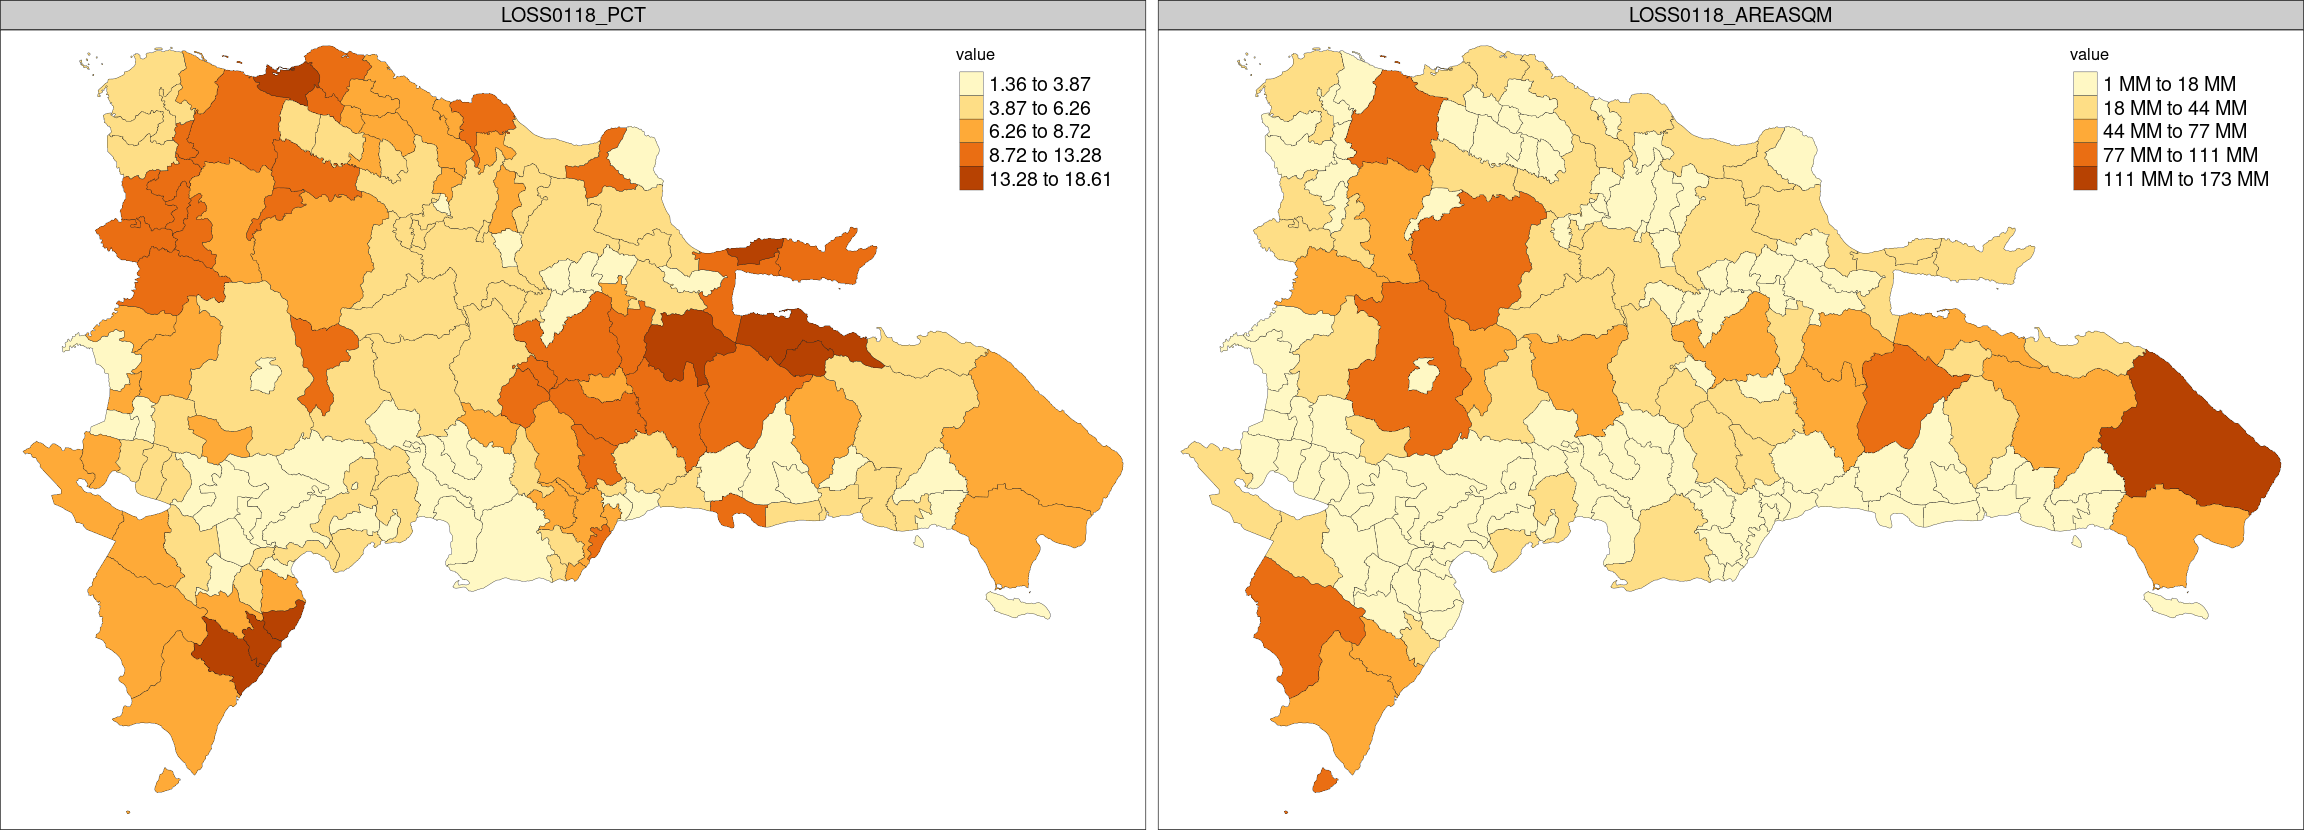
\includegraphics{img/data-download-preparation-eda/zonal-mun-4} \end{center}

\begin{Shaded}
\begin{Highlighting}[]
\CommentTok{\# Top twenty sorted descending by column 2}
\FunctionTok{stripped\_table}\NormalTok{(munzonal }\SpecialCharTok{\%\textgreater{}\%} \FunctionTok{select}\NormalTok{(TOPONIMIA, }\FunctionTok{matches}\NormalTok{(}\StringTok{\textquotesingle{}\^{}LOSS0118\textquotesingle{}}\NormalTok{)) }\SpecialCharTok{\%\textgreater{}\%} \FunctionTok{select}\NormalTok{(}\SpecialCharTok{{-}}\FunctionTok{matches}\NormalTok{(}\StringTok{\textquotesingle{}\textless{}NA\textgreater{}\textquotesingle{}}\NormalTok{)))}
\end{Highlighting}
\end{Shaded}

\begin{table}[H]
\centering
\begin{tabular}[t]{llrr}
\toprule
  & TOPONIMIA & LOSS0118\_PCT & LOSS0118\_AREASQM\\
\midrule
\cellcolor{lightgray}{1} & \cellcolor{lightgray}{LAS TERRENAS} & \cellcolor{lightgray}{18.60592} & \cellcolor{lightgray}{20803822}\\
2 & ENRIQUILLO & 18.15716 & 59584385\\
\cellcolor{lightgray}{3} & \cellcolor{lightgray}{VILLA ISABELA} & \cellcolor{lightgray}{17.06917} & \cellcolor{lightgray}{36146513}\\
4 & EL VALLE & 16.79842 & 27327732\\
\cellcolor{lightgray}{5} & \cellcolor{lightgray}{LA CIÉNAGA} & \cellcolor{lightgray}{15.10272} & \cellcolor{lightgray}{17650896}\\
\addlinespace
6 & PARAÍSO & 15.00678 & 20434419\\
\cellcolor{lightgray}{7} & \cellcolor{lightgray}{SABANA GRANDE DE BOYÁ} & \cellcolor{lightgray}{14.32006} & \cellcolor{lightgray}{75546364}\\
8 & SABANA DE LA MAR & 13.85536 & 70839509\\
\cellcolor{lightgray}{9} & \cellcolor{lightgray}{LOMA DE CABRERA} & \cellcolor{lightgray}{13.27824} & \cellcolor{lightgray}{32730761}\\
10 & BAYAGUANA & 12.71269 & 110973740\\
\addlinespace
\cellcolor{lightgray}{11} & \cellcolor{lightgray}{VILLA LOS ALMÁCIGOS} & \cellcolor{lightgray}{12.49025} & \cellcolor{lightgray}{25906886}\\
12 & BOHECHÍO & 11.96513 & 48596055\\
\cellcolor{lightgray}{13} & \cellcolor{lightgray}{RESTAURACIÓN} & \cellcolor{lightgray}{11.95832} & \cellcolor{lightgray}{33003809}\\
14 & EL PINO & 11.77891 & 10334479\\
\cellcolor{lightgray}{15} & \cellcolor{lightgray}{LAS MATAS DE SANTA CRUZ} & \cellcolor{lightgray}{11.74594} & \cellcolor{lightgray}{8424526}\\
\addlinespace
16 & COTUÍ & 11.62869 & 76879543\\
\cellcolor{lightgray}{17} & \cellcolor{lightgray}{PEDRO BRAND} & \cellcolor{lightgray}{11.51339} & \cellcolor{lightgray}{25532014}\\
18 & SOSÚA & 11.00357 & 29431673\\
\cellcolor{lightgray}{19} & \cellcolor{lightgray}{PEDRO SANTANA} & \cellcolor{lightgray}{10.95457} & \cellcolor{lightgray}{60055728}\\
20 & PARTIDO & 10.84866 & 16249652\\
\bottomrule
\end{tabular}
\end{table}

\begin{Shaded}
\begin{Highlighting}[]

\CommentTok{\# Total loss 2012{-}2018}
\NormalTok{munzonal }\SpecialCharTok{\%\textgreater{}\%} \FunctionTok{select}\NormalTok{(}\FunctionTok{matches}\NormalTok{(}\StringTok{\textquotesingle{}\^{}LOSS1218\textquotesingle{}}\NormalTok{)) }\SpecialCharTok{\%\textgreater{}\%} \FunctionTok{select}\NormalTok{(}\SpecialCharTok{{-}}\FunctionTok{matches}\NormalTok{(}\StringTok{\textquotesingle{}\textless{}NA\textgreater{}\textquotesingle{}}\NormalTok{)) }\SpecialCharTok{\%\textgreater{}\%} 
  \FunctionTok{gather}\NormalTok{(variable, value, }\SpecialCharTok{{-}}\NormalTok{geom) }\SpecialCharTok{\%\textgreater{}\%}
  \FunctionTok{mutate}\NormalTok{(}\AttributeTok{variable =} \FunctionTok{factor}\NormalTok{(variable, }\AttributeTok{levels =} \FunctionTok{unique}\NormalTok{(variable))) }\SpecialCharTok{\%\textgreater{}\%} 
  \FunctionTok{tm\_shape}\NormalTok{() }\SpecialCharTok{+}
    \FunctionTok{tm\_fill}\NormalTok{(}\AttributeTok{col=}\StringTok{\textquotesingle{}value\textquotesingle{}}\NormalTok{, }\AttributeTok{palette =} \StringTok{"YlOrBr"}\NormalTok{, }\AttributeTok{size =} \FloatTok{0.1}\NormalTok{, }\AttributeTok{style =} \StringTok{\textquotesingle{}jenks\textquotesingle{}}\NormalTok{) }\SpecialCharTok{+}
    \FunctionTok{tm\_borders}\NormalTok{(}\AttributeTok{col =} \StringTok{\textquotesingle{}grey15\textquotesingle{}}\NormalTok{, }\AttributeTok{lwd =} \FloatTok{0.3}\NormalTok{) }\SpecialCharTok{+}
    \FunctionTok{tm\_facets}\NormalTok{(}\AttributeTok{by =} \StringTok{"variable"}\NormalTok{, }\AttributeTok{ncol =} \DecValTok{2}\NormalTok{, }\AttributeTok{nrow =} \DecValTok{1}\NormalTok{, }\AttributeTok{free.coords =} \ConstantTok{FALSE}\NormalTok{, }\AttributeTok{free.scales =} \ConstantTok{TRUE}\NormalTok{) }\SpecialCharTok{+}
    \FunctionTok{tm\_layout}\NormalTok{(}\AttributeTok{panel.label.size =} \DecValTok{1}\NormalTok{, }\AttributeTok{legend.title.size =} \DecValTok{1}\NormalTok{, }\AttributeTok{legend.text.size =} \DecValTok{1}\NormalTok{)}
\end{Highlighting}
\end{Shaded}

\begin{center}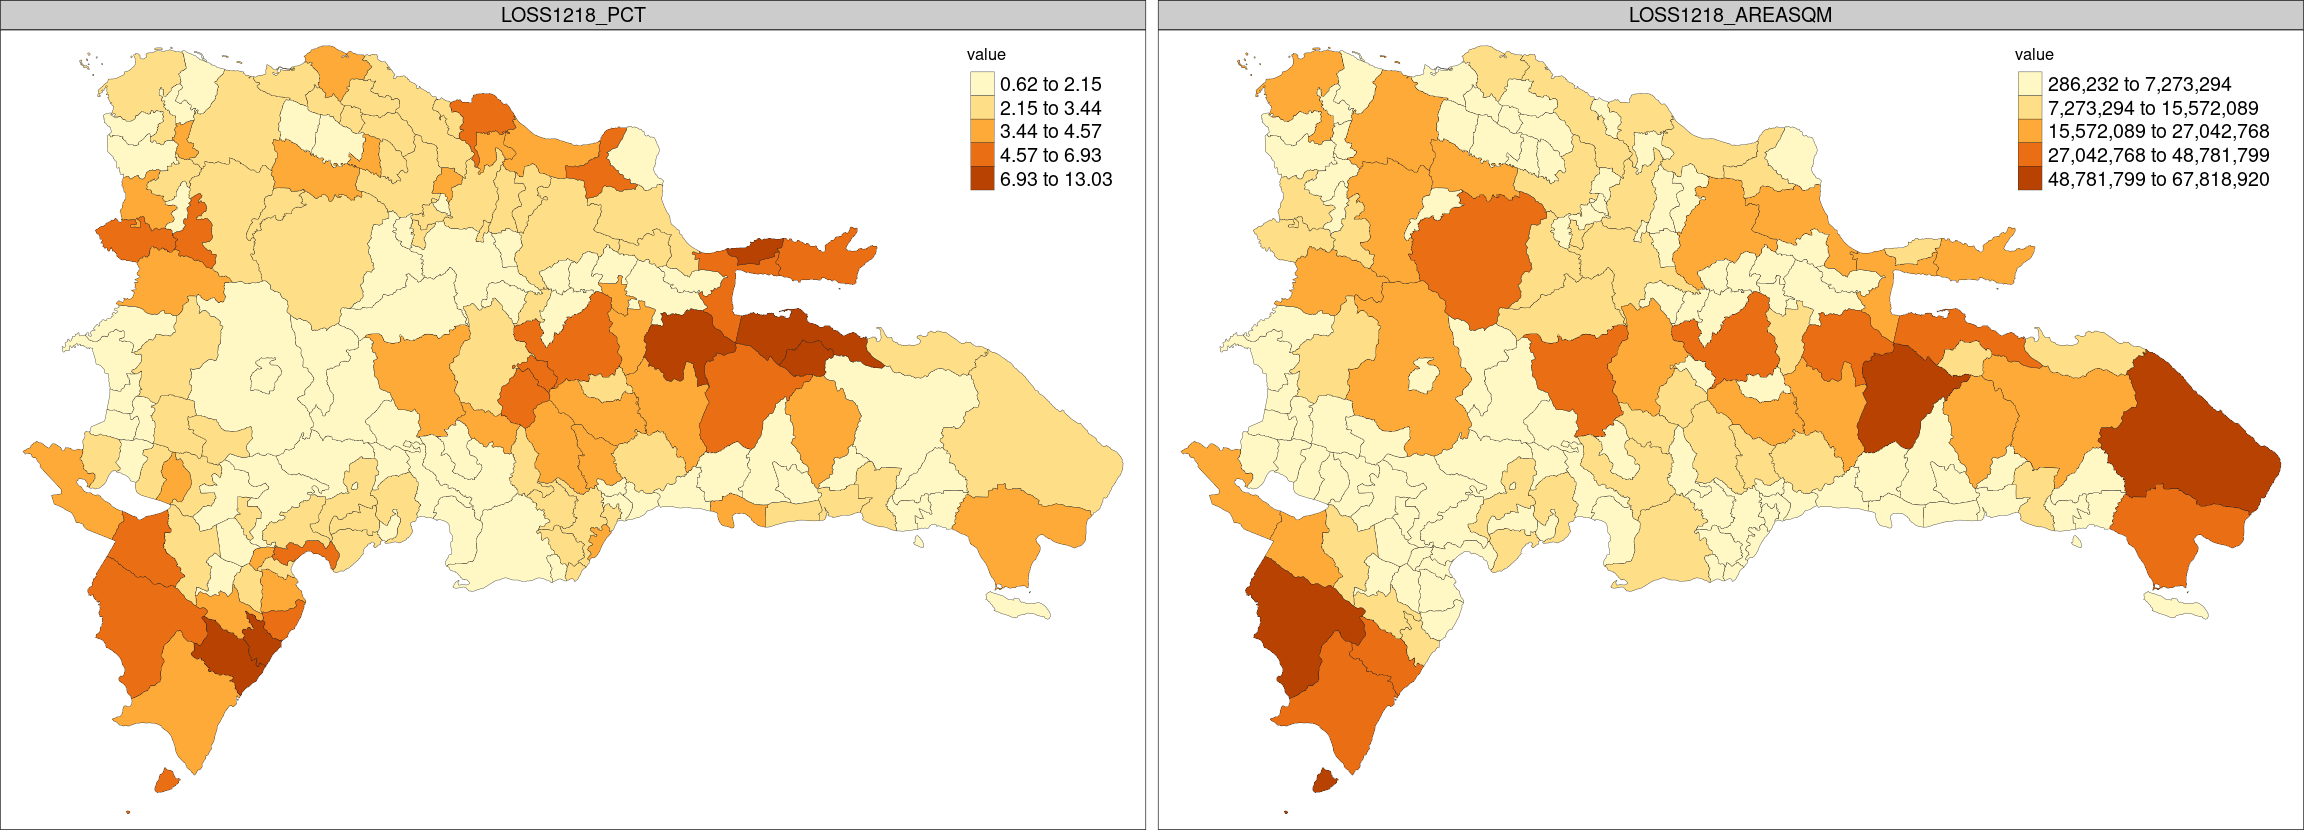
\includegraphics{img/data-download-preparation-eda/zonal-mun-5} \end{center}

\begin{Shaded}
\begin{Highlighting}[]
\CommentTok{\# Top twenty sorted descending by column 2}
\FunctionTok{stripped\_table}\NormalTok{(munzonal }\SpecialCharTok{\%\textgreater{}\%} \FunctionTok{select}\NormalTok{(TOPONIMIA, }\FunctionTok{matches}\NormalTok{(}\StringTok{\textquotesingle{}\^{}LOSS1218\textquotesingle{}}\NormalTok{)) }\SpecialCharTok{\%\textgreater{}\%} \FunctionTok{select}\NormalTok{(}\SpecialCharTok{{-}}\FunctionTok{matches}\NormalTok{(}\StringTok{\textquotesingle{}\textless{}NA\textgreater{}\textquotesingle{}}\NormalTok{)))}
\end{Highlighting}
\end{Shaded}

\begin{table}[H]
\centering
\begin{tabular}[t]{llrr}
\toprule
  & TOPONIMIA & LOSS1218\_PCT & LOSS1218\_AREASQM\\
\midrule
\cellcolor{lightgray}{1} & \cellcolor{lightgray}{LAS TERRENAS} & \cellcolor{lightgray}{13.025658} & \cellcolor{lightgray}{14564368}\\
2 & ENRIQUILLO & 9.687927 & 31791827\\
\cellcolor{lightgray}{3} & \cellcolor{lightgray}{SABANA DE LA MAR} & \cellcolor{lightgray}{9.541138} & \cellcolor{lightgray}{48781799}\\
4 & SABANA GRANDE DE BOYÁ & 8.643936 & 45601628\\
\cellcolor{lightgray}{5} & \cellcolor{lightgray}{PARAÍSO} & \cellcolor{lightgray}{8.500673} & \cellcolor{lightgray}{11575189}\\
\addlinespace
6 & EL VALLE & 7.944483 & 12924115\\
\cellcolor{lightgray}{7} & \cellcolor{lightgray}{BAYAGUANA} & \cellcolor{lightgray}{6.931707} & \cellcolor{lightgray}{60509395}\\
8 & SÁNCHEZ & 6.359689 & 21658175\\
\cellcolor{lightgray}{9} & \cellcolor{lightgray}{MAIMÓN} & \cellcolor{lightgray}{6.338366} & \cellcolor{lightgray}{5242823}\\
10 & SAMANÁ & 6.082577 & 24977993\\
\addlinespace
\cellcolor{lightgray}{11} & \cellcolor{lightgray}{PIEDRA BLANCA} & \cellcolor{lightgray}{5.899492} & \cellcolor{lightgray}{13644958}\\
12 & COTUÍ & 5.797430 & 38327951\\
\cellcolor{lightgray}{13} & \cellcolor{lightgray}{LA CIÉNAGA} & \cellcolor{lightgray}{5.664938} & \cellcolor{lightgray}{6620741}\\
14 & RESTAURACIÓN & 5.468702 & 15093089\\
\cellcolor{lightgray}{15} & \cellcolor{lightgray}{RÍO SAN JUAN} & \cellcolor{lightgray}{5.459185} & \cellcolor{lightgray}{13348448}\\
\addlinespace
16 & SOSÚA & 5.345556 & 14297969\\
\cellcolor{lightgray}{17} & \cellcolor{lightgray}{PEDERNALES} & \cellcolor{lightgray}{5.098481} & \cellcolor{lightgray}{57127986}\\
18 & DUVERGÉ & 4.993313 & 22026878\\
\cellcolor{lightgray}{19} & \cellcolor{lightgray}{VILLA LOS ALMÁCIGOS} & \cellcolor{lightgray}{4.946938} & \cellcolor{lightgray}{10260787}\\
20 & JAQUIMEYES & 4.932285 & 5672865\\
\bottomrule
\end{tabular}
\end{table}

\begin{Shaded}
\begin{Highlighting}[]

\CommentTok{\# Fires M6}
\NormalTok{munzonal }\SpecialCharTok{\%\textgreater{}\%} \FunctionTok{select}\NormalTok{(}\FunctionTok{matches}\NormalTok{(}\StringTok{\textquotesingle{}\^{}LOSS0118|NFIRESM6\textquotesingle{}}\NormalTok{)) }\SpecialCharTok{\%\textgreater{}\%} \FunctionTok{select}\NormalTok{(}\SpecialCharTok{{-}}\FunctionTok{matches}\NormalTok{(}\StringTok{\textquotesingle{}\textless{}NA\textgreater{}\textquotesingle{}}\NormalTok{)) }\SpecialCharTok{\%\textgreater{}\%} 
  \FunctionTok{gather}\NormalTok{(variable, value, }\SpecialCharTok{{-}}\NormalTok{geom) }\SpecialCharTok{\%\textgreater{}\%}
  \FunctionTok{mutate}\NormalTok{(}\AttributeTok{variable =} \FunctionTok{factor}\NormalTok{(variable, }\AttributeTok{levels =} \FunctionTok{unique}\NormalTok{(variable))) }\SpecialCharTok{\%\textgreater{}\%} 
  \FunctionTok{tm\_shape}\NormalTok{() }\SpecialCharTok{+}
  \FunctionTok{tm\_fill}\NormalTok{(}\AttributeTok{col=}\StringTok{\textquotesingle{}value\textquotesingle{}}\NormalTok{, }\AttributeTok{palette =} \StringTok{"YlOrBr"}\NormalTok{, }\AttributeTok{size =} \FloatTok{0.1}\NormalTok{, }\AttributeTok{style =} \StringTok{\textquotesingle{}jenks\textquotesingle{}}\NormalTok{) }\SpecialCharTok{+}
  \FunctionTok{tm\_borders}\NormalTok{(}\AttributeTok{col =} \StringTok{\textquotesingle{}grey15\textquotesingle{}}\NormalTok{, }\AttributeTok{lwd =} \FloatTok{0.3}\NormalTok{) }\SpecialCharTok{+}
  \FunctionTok{tm\_facets}\NormalTok{(}\AttributeTok{by =} \StringTok{"variable"}\NormalTok{, }\AttributeTok{ncol =} \DecValTok{3}\NormalTok{, }\AttributeTok{nrow =} \DecValTok{1}\NormalTok{, }\AttributeTok{free.coords =} \ConstantTok{FALSE}\NormalTok{, }\AttributeTok{free.scales =} \ConstantTok{TRUE}\NormalTok{) }\SpecialCharTok{+}
  \FunctionTok{tm\_layout}\NormalTok{(}\AttributeTok{panel.label.size =} \DecValTok{1}\NormalTok{, }\AttributeTok{legend.title.size =} \DecValTok{1}\NormalTok{, }\AttributeTok{legend.text.size =} \DecValTok{1}\NormalTok{)}
\end{Highlighting}
\end{Shaded}

\begin{center}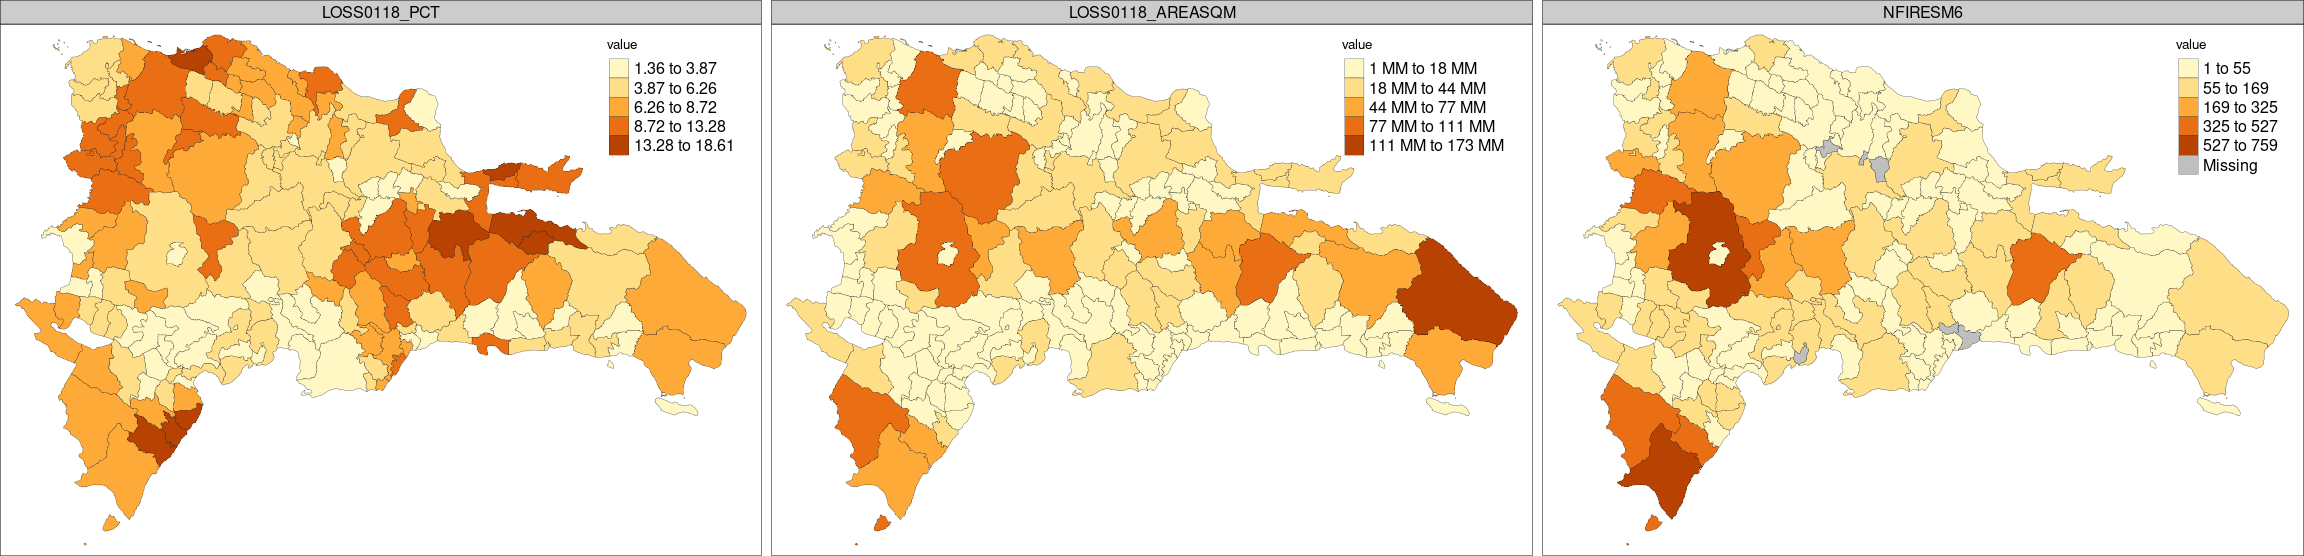
\includegraphics{img/data-download-preparation-eda/zonal-mun-6} \end{center}

\begin{Shaded}
\begin{Highlighting}[]
\CommentTok{\# Top twenty sorted descending by column 2}
\FunctionTok{stripped\_table}\NormalTok{(munzonal }\SpecialCharTok{\%\textgreater{}\%} \FunctionTok{select}\NormalTok{(TOPONIMIA, }\FunctionTok{matches}\NormalTok{(}\StringTok{\textquotesingle{}\^{}LOSS0118|NFIRESM6\textquotesingle{}}\NormalTok{)) }\SpecialCharTok{\%\textgreater{}\%} \FunctionTok{select}\NormalTok{(}\SpecialCharTok{{-}}\FunctionTok{matches}\NormalTok{(}\StringTok{\textquotesingle{}\textless{}NA\textgreater{}\textquotesingle{}}\NormalTok{)))}
\end{Highlighting}
\end{Shaded}

\begin{table}[H]
\centering
\begin{tabular}[t]{llrrr}
\toprule
  & TOPONIMIA & LOSS0118\_PCT & LOSS0118\_AREASQM & NFIRESM6\\
\midrule
\cellcolor{lightgray}{1} & \cellcolor{lightgray}{LAS TERRENAS} & \cellcolor{lightgray}{18.60592} & \cellcolor{lightgray}{20803822} & \cellcolor{lightgray}{68}\\
2 & ENRIQUILLO & 18.15716 & 59584385 & 463\\
\cellcolor{lightgray}{3} & \cellcolor{lightgray}{VILLA ISABELA} & \cellcolor{lightgray}{17.06917} & \cellcolor{lightgray}{36146513} & \cellcolor{lightgray}{49}\\
4 & EL VALLE & 16.79842 & 27327732 & 26\\
\cellcolor{lightgray}{5} & \cellcolor{lightgray}{LA CIÉNAGA} & \cellcolor{lightgray}{15.10272} & \cellcolor{lightgray}{17650896} & \cellcolor{lightgray}{71}\\
\addlinespace
6 & PARAÍSO & 15.00678 & 20434419 & 28\\
\cellcolor{lightgray}{7} & \cellcolor{lightgray}{SABANA GRANDE DE BOYÁ} & \cellcolor{lightgray}{14.32006} & \cellcolor{lightgray}{75546364} & \cellcolor{lightgray}{155}\\
8 & SABANA DE LA MAR & 13.85536 & 70839509 & 102\\
\cellcolor{lightgray}{9} & \cellcolor{lightgray}{LOMA DE CABRERA} & \cellcolor{lightgray}{13.27824} & \cellcolor{lightgray}{32730761} & \cellcolor{lightgray}{89}\\
10 & BAYAGUANA & 12.71269 & 110973740 & 422\\
\addlinespace
\cellcolor{lightgray}{11} & \cellcolor{lightgray}{VILLA LOS ALMÁCIGOS} & \cellcolor{lightgray}{12.49025} & \cellcolor{lightgray}{25906886} & \cellcolor{lightgray}{109}\\
12 & BOHECHÍO & 11.96513 & 48596055 & 527\\
\cellcolor{lightgray}{13} & \cellcolor{lightgray}{RESTAURACIÓN} & \cellcolor{lightgray}{11.95832} & \cellcolor{lightgray}{33003809} & \cellcolor{lightgray}{203}\\
14 & EL PINO & 11.77891 & 10334479 & 28\\
\cellcolor{lightgray}{15} & \cellcolor{lightgray}{LAS MATAS DE SANTA CRUZ} & \cellcolor{lightgray}{11.74594} & \cellcolor{lightgray}{8424526} & \cellcolor{lightgray}{27}\\
\addlinespace
16 & COTUÍ & 11.62869 & 76879543 & 136\\
\cellcolor{lightgray}{17} & \cellcolor{lightgray}{PEDRO BRAND} & \cellcolor{lightgray}{11.51339} & \cellcolor{lightgray}{25532014} & \cellcolor{lightgray}{132}\\
18 & SOSÚA & 11.00357 & 29431673 & 54\\
\cellcolor{lightgray}{19} & \cellcolor{lightgray}{PEDRO SANTANA} & \cellcolor{lightgray}{10.95457} & \cellcolor{lightgray}{60055728} & \cellcolor{lightgray}{430}\\
20 & PARTIDO & 10.84866 & 16249652 & 81\\
\bottomrule
\end{tabular}
\end{table}

\begin{Shaded}
\begin{Highlighting}[]

\CommentTok{\# Fires M6. Only AREASQM and FIRESM6}
\NormalTok{munzonal }\SpecialCharTok{\%\textgreater{}\%} \FunctionTok{select}\NormalTok{(}\FunctionTok{matches}\NormalTok{(}\StringTok{\textquotesingle{}\^{}LOSS0118\_AREASQM|NFIRESM6|TOPONIMIA\textquotesingle{}}\NormalTok{)) }\SpecialCharTok{\%\textgreater{}\%} \FunctionTok{select}\NormalTok{(}\SpecialCharTok{{-}}\FunctionTok{matches}\NormalTok{(}\StringTok{\textquotesingle{}\textless{}NA\textgreater{}\textquotesingle{}}\NormalTok{)) }\SpecialCharTok{\%\textgreater{}\%} 
  \FunctionTok{gather}\NormalTok{(variable, value, }\SpecialCharTok{{-}}\NormalTok{geom, }\SpecialCharTok{{-}}\NormalTok{TOPONIMIA) }\SpecialCharTok{\%\textgreater{}\%}
  \FunctionTok{mutate}\NormalTok{(}\AttributeTok{TOPONIMIA=}\FunctionTok{gsub}\NormalTok{(}\StringTok{\textquotesingle{} \textquotesingle{}}\NormalTok{, }\StringTok{\textquotesingle{}}\SpecialCharTok{\textbackslash{}n}\StringTok{\textquotesingle{}}\NormalTok{, TOPONIMIA)) }\SpecialCharTok{\%\textgreater{}\%} 
  \FunctionTok{mutate}\NormalTok{(}\AttributeTok{variable =} \FunctionTok{factor}\NormalTok{(variable, }\AttributeTok{levels =} \FunctionTok{unique}\NormalTok{(variable))) }\SpecialCharTok{\%\textgreater{}\%} 
  \FunctionTok{tm\_shape}\NormalTok{() }\SpecialCharTok{+}
  \FunctionTok{tm\_fill}\NormalTok{(}\AttributeTok{col=}\StringTok{\textquotesingle{}value\textquotesingle{}}\NormalTok{, }\AttributeTok{palette =} \StringTok{"YlOrBr"}\NormalTok{, }\AttributeTok{size =} \FloatTok{0.1}\NormalTok{, }\AttributeTok{style =} \StringTok{\textquotesingle{}jenks\textquotesingle{}}\NormalTok{) }\SpecialCharTok{+}
  \FunctionTok{tm\_borders}\NormalTok{(}\AttributeTok{col =} \StringTok{\textquotesingle{}grey15\textquotesingle{}}\NormalTok{, }\AttributeTok{lwd =} \FloatTok{0.3}\NormalTok{) }\SpecialCharTok{+}
  \FunctionTok{tm\_facets}\NormalTok{(}\AttributeTok{by =} \StringTok{"variable"}\NormalTok{, }\AttributeTok{ncol =} \DecValTok{2}\NormalTok{, }\AttributeTok{nrow =} \DecValTok{1}\NormalTok{, }\AttributeTok{free.coords =} \ConstantTok{FALSE}\NormalTok{, }\AttributeTok{free.scales =} \ConstantTok{TRUE}\NormalTok{) }\SpecialCharTok{+}
  \FunctionTok{tm\_layout}\NormalTok{(}\AttributeTok{panel.label.size =} \DecValTok{1}\NormalTok{, }\AttributeTok{legend.title.size =} \DecValTok{1}\NormalTok{, }\AttributeTok{legend.text.size =} \DecValTok{1}\NormalTok{) }\SpecialCharTok{+}
  \FunctionTok{tm\_text}\NormalTok{(}\AttributeTok{text =} \StringTok{\textquotesingle{}TOPONIMIA\textquotesingle{}}\NormalTok{, }\AttributeTok{size =} \FloatTok{0.5}\NormalTok{)}
\end{Highlighting}
\end{Shaded}

\begin{center}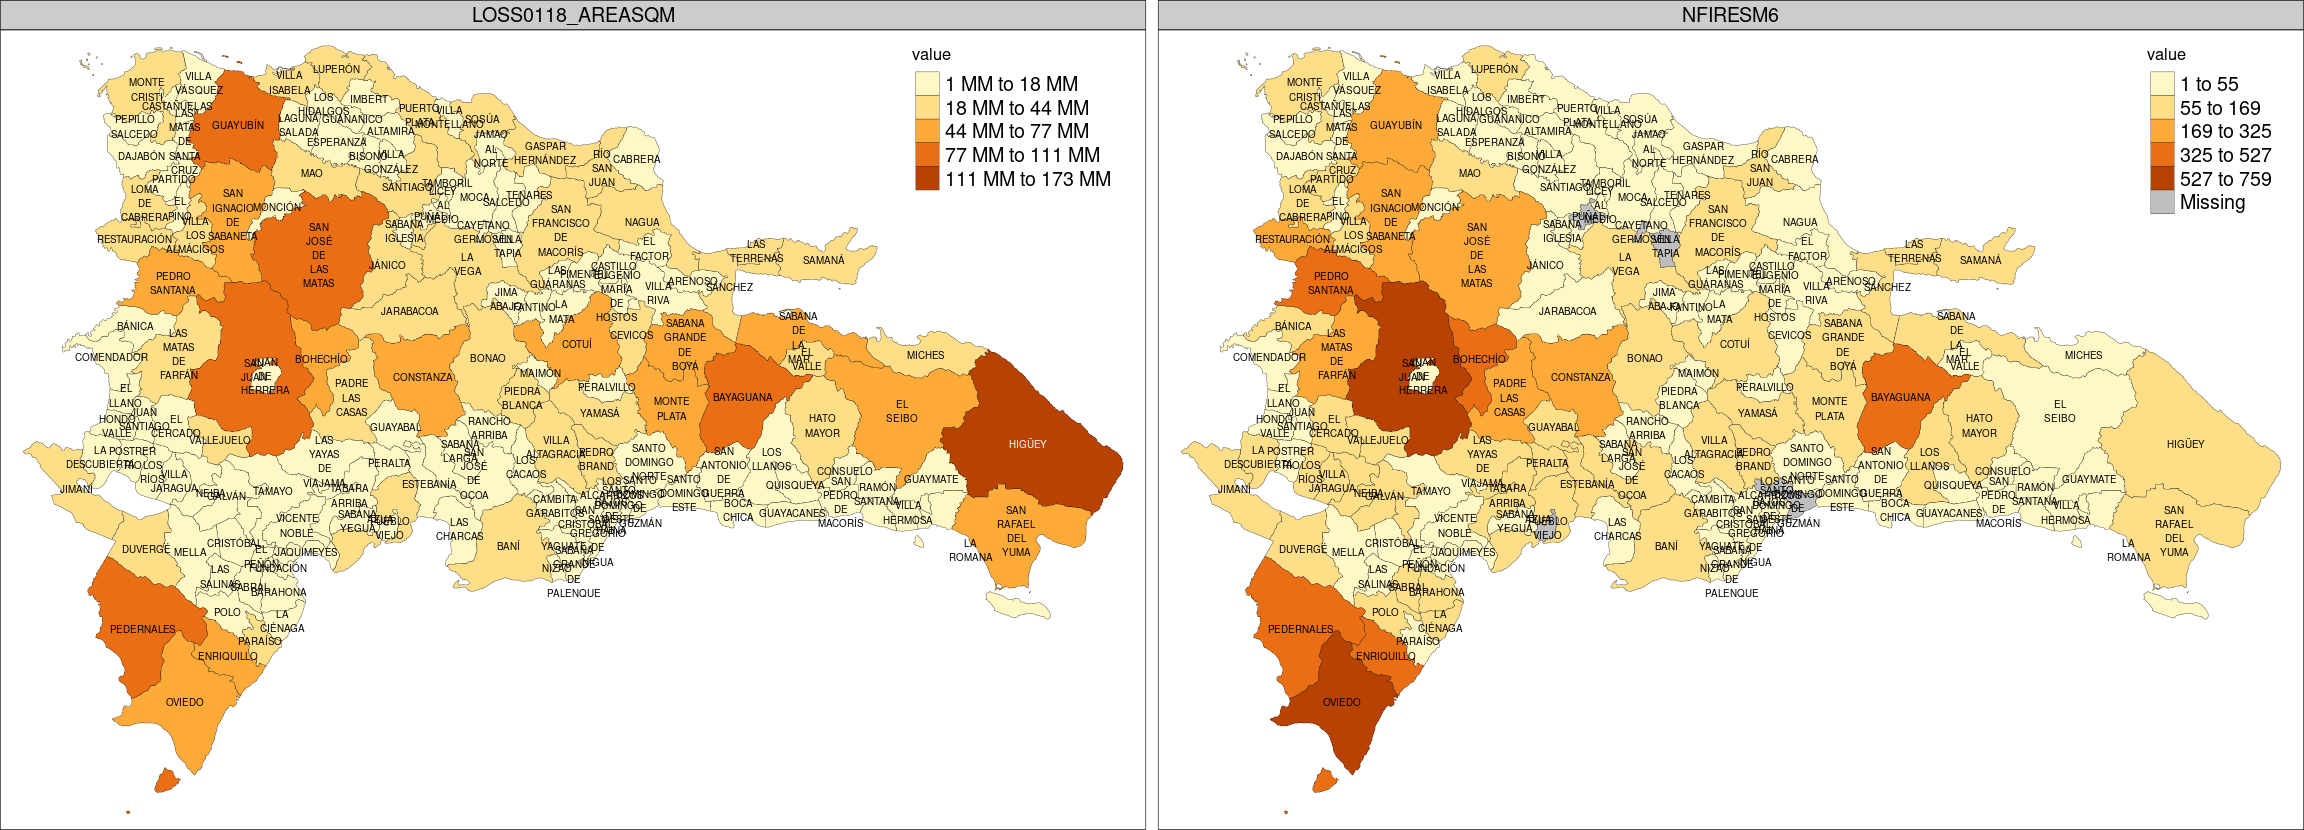
\includegraphics{img/data-download-preparation-eda/zonal-mun-7} \end{center}

\begin{Shaded}
\begin{Highlighting}[]
\CommentTok{\# Top twenty sorted descending by column 2}
\FunctionTok{stripped\_table}\NormalTok{(munzonal }\SpecialCharTok{\%\textgreater{}\%} \FunctionTok{select}\NormalTok{(TOPONIMIA, }\FunctionTok{matches}\NormalTok{(}\StringTok{\textquotesingle{}\^{}LOSS0118\_AREASQM|NFIRESM6|TOPONIMIA\textquotesingle{}}\NormalTok{)) }\SpecialCharTok{\%\textgreater{}\%} \FunctionTok{select}\NormalTok{(}\SpecialCharTok{{-}}\FunctionTok{matches}\NormalTok{(}\StringTok{\textquotesingle{}\textless{}NA\textgreater{}\textquotesingle{}}\NormalTok{)))}
\end{Highlighting}
\end{Shaded}

\begin{table}[H]
\centering
\begin{tabular}[t]{llrr}
\toprule
  & TOPONIMIA & LOSS0118\_AREASQM & NFIRESM6\\
\midrule
\cellcolor{lightgray}{1} & \cellcolor{lightgray}{HIGÜEY} & \cellcolor{lightgray}{172531196} & \cellcolor{lightgray}{121}\\
2 & BAYAGUANA & 110973740 & 422\\
\cellcolor{lightgray}{3} & \cellcolor{lightgray}{SAN JOSÉ DE LAS MATAS} & \cellcolor{lightgray}{100892170} & \cellcolor{lightgray}{299}\\
4 & SAN JUAN & 95509530 & 759\\
\cellcolor{lightgray}{5} & \cellcolor{lightgray}{PEDERNALES} & \cellcolor{lightgray}{95166718} & \cellcolor{lightgray}{413}\\
\addlinespace
6 & GUAYUBÍN & 85736587 & 325\\
\cellcolor{lightgray}{7} & \cellcolor{lightgray}{COTUÍ} & \cellcolor{lightgray}{76879543} & \cellcolor{lightgray}{136}\\
8 & SAN RAFAEL DEL YUMA & 76759362 & 109\\
\cellcolor{lightgray}{9} & \cellcolor{lightgray}{SABANA GRANDE DE BOYÁ} & \cellcolor{lightgray}{75546364} & \cellcolor{lightgray}{155}\\
10 & SABANA DE LA MAR & 70839509 & 102\\
\addlinespace
\cellcolor{lightgray}{11} & \cellcolor{lightgray}{OVIEDO} & \cellcolor{lightgray}{67603535} & \cellcolor{lightgray}{599}\\
12 & EL SEIBO & 63022977 & 55\\
\cellcolor{lightgray}{13} & \cellcolor{lightgray}{SAN IGNACIO DE SABANETA} & \cellcolor{lightgray}{61756747} & \cellcolor{lightgray}{202}\\
14 & MONTE PLATA & 60527072 & 82\\
\cellcolor{lightgray}{15} & \cellcolor{lightgray}{PEDRO SANTANA} & \cellcolor{lightgray}{60055728} & \cellcolor{lightgray}{430}\\
\addlinespace
16 & ENRIQUILLO & 59584385 & 463\\
\cellcolor{lightgray}{17} & \cellcolor{lightgray}{CONSTANZA} & \cellcolor{lightgray}{48663568} & \cellcolor{lightgray}{299}\\
18 & BOHECHÍO & 48596055 & 527\\
\cellcolor{lightgray}{19} & \cellcolor{lightgray}{YAMASÁ} & \cellcolor{lightgray}{44179210} & \cellcolor{lightgray}{117}\\
20 & SAMANÁ & 42187655 & 73\\
\bottomrule
\end{tabular}
\end{table}

\begin{Shaded}
\begin{Highlighting}[]

\CommentTok{\# Fires V1}
\NormalTok{munzonal }\SpecialCharTok{\%\textgreater{}\%} \FunctionTok{select}\NormalTok{(}\FunctionTok{matches}\NormalTok{(}\StringTok{\textquotesingle{}\^{}LOSS1218|NFIRESV1\textquotesingle{}}\NormalTok{)) }\SpecialCharTok{\%\textgreater{}\%} \FunctionTok{select}\NormalTok{(}\SpecialCharTok{{-}}\FunctionTok{matches}\NormalTok{(}\StringTok{\textquotesingle{}\textless{}NA\textgreater{}\textquotesingle{}}\NormalTok{)) }\SpecialCharTok{\%\textgreater{}\%} 
  \FunctionTok{gather}\NormalTok{(variable, value, }\SpecialCharTok{{-}}\NormalTok{geom) }\SpecialCharTok{\%\textgreater{}\%}
  \FunctionTok{mutate}\NormalTok{(}\AttributeTok{variable =} \FunctionTok{factor}\NormalTok{(variable, }\AttributeTok{levels =} \FunctionTok{unique}\NormalTok{(variable))) }\SpecialCharTok{\%\textgreater{}\%} 
  \FunctionTok{tm\_shape}\NormalTok{() }\SpecialCharTok{+}
  \FunctionTok{tm\_fill}\NormalTok{(}\AttributeTok{col=}\StringTok{\textquotesingle{}value\textquotesingle{}}\NormalTok{, }\AttributeTok{palette =} \StringTok{"YlOrBr"}\NormalTok{, }\AttributeTok{size =} \FloatTok{0.1}\NormalTok{, }\AttributeTok{style =} \StringTok{\textquotesingle{}jenks\textquotesingle{}}\NormalTok{) }\SpecialCharTok{+}
  \FunctionTok{tm\_borders}\NormalTok{(}\AttributeTok{col =} \StringTok{\textquotesingle{}grey15\textquotesingle{}}\NormalTok{, }\AttributeTok{lwd =} \FloatTok{0.3}\NormalTok{) }\SpecialCharTok{+}
  \FunctionTok{tm\_facets}\NormalTok{(}\AttributeTok{by =} \StringTok{"variable"}\NormalTok{, }\AttributeTok{ncol =} \DecValTok{3}\NormalTok{, }\AttributeTok{nrow =} \DecValTok{1}\NormalTok{, }\AttributeTok{free.coords =} \ConstantTok{FALSE}\NormalTok{, }\AttributeTok{free.scales =} \ConstantTok{TRUE}\NormalTok{) }\SpecialCharTok{+}
  \FunctionTok{tm\_layout}\NormalTok{(}\AttributeTok{panel.label.size =} \DecValTok{1}\NormalTok{, }\AttributeTok{legend.title.size =} \DecValTok{1}\NormalTok{, }\AttributeTok{legend.text.size =} \DecValTok{1}\NormalTok{)}
\end{Highlighting}
\end{Shaded}

\begin{center}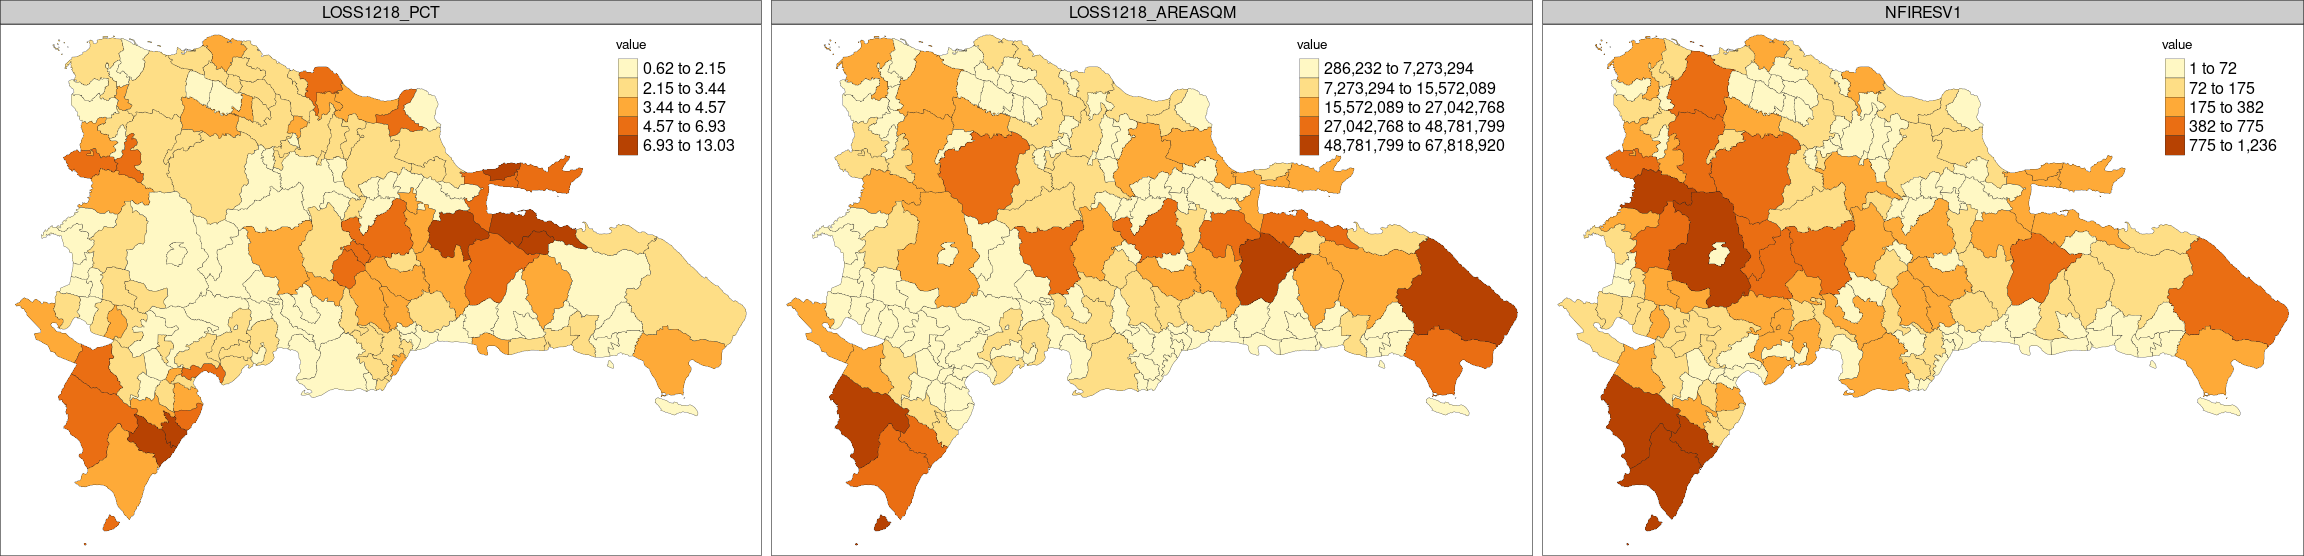
\includegraphics{img/data-download-preparation-eda/zonal-mun-8} \end{center}

\begin{Shaded}
\begin{Highlighting}[]
\CommentTok{\# Top twenty sorted descending by column 2}
\FunctionTok{stripped\_table}\NormalTok{(munzonal }\SpecialCharTok{\%\textgreater{}\%} \FunctionTok{select}\NormalTok{(TOPONIMIA, }\FunctionTok{matches}\NormalTok{(}\StringTok{\textquotesingle{}\^{}LOSS1218|NFIRESV1\textquotesingle{}}\NormalTok{)) }\SpecialCharTok{\%\textgreater{}\%} \FunctionTok{select}\NormalTok{(}\SpecialCharTok{{-}}\FunctionTok{matches}\NormalTok{(}\StringTok{\textquotesingle{}\textless{}NA\textgreater{}\textquotesingle{}}\NormalTok{)))}
\end{Highlighting}
\end{Shaded}

\begin{table}[H]
\centering
\begin{tabular}[t]{llrrr}
\toprule
  & TOPONIMIA & LOSS1218\_PCT & LOSS1218\_AREASQM & NFIRESV1\\
\midrule
\cellcolor{lightgray}{1} & \cellcolor{lightgray}{LAS TERRENAS} & \cellcolor{lightgray}{13.025658} & \cellcolor{lightgray}{14564368} & \cellcolor{lightgray}{261}\\
2 & ENRIQUILLO & 9.687927 & 31791827 & 981\\
\cellcolor{lightgray}{3} & \cellcolor{lightgray}{SABANA DE LA MAR} & \cellcolor{lightgray}{9.541138} & \cellcolor{lightgray}{48781799} & \cellcolor{lightgray}{355}\\
4 & SABANA GRANDE DE BOYÁ & 8.643936 & 45601628 & 382\\
\cellcolor{lightgray}{5} & \cellcolor{lightgray}{PARAÍSO} & \cellcolor{lightgray}{8.500673} & \cellcolor{lightgray}{11575189} & \cellcolor{lightgray}{100}\\
\addlinespace
6 & EL VALLE & 7.944483 & 12924115 & 67\\
\cellcolor{lightgray}{7} & \cellcolor{lightgray}{BAYAGUANA} & \cellcolor{lightgray}{6.931707} & \cellcolor{lightgray}{60509395} & \cellcolor{lightgray}{775}\\
8 & SÁNCHEZ & 6.359689 & 21658175 & 284\\
\cellcolor{lightgray}{9} & \cellcolor{lightgray}{MAIMÓN} & \cellcolor{lightgray}{6.338366} & \cellcolor{lightgray}{5242823} & \cellcolor{lightgray}{28}\\
10 & SAMANÁ & 6.082577 & 24977993 & 290\\
\addlinespace
\cellcolor{lightgray}{11} & \cellcolor{lightgray}{PIEDRA BLANCA} & \cellcolor{lightgray}{5.899492} & \cellcolor{lightgray}{13644958} & \cellcolor{lightgray}{126}\\
12 & COTUÍ & 5.797430 & 38327951 & 256\\
\cellcolor{lightgray}{13} & \cellcolor{lightgray}{LA CIÉNAGA} & \cellcolor{lightgray}{5.664938} & \cellcolor{lightgray}{6620741} & \cellcolor{lightgray}{160}\\
14 & RESTAURACIÓN & 5.468702 & 15093089 & 484\\
\cellcolor{lightgray}{15} & \cellcolor{lightgray}{RÍO SAN JUAN} & \cellcolor{lightgray}{5.459185} & \cellcolor{lightgray}{13348448} & \cellcolor{lightgray}{120}\\
\addlinespace
16 & SOSÚA & 5.345556 & 14297969 & 211\\
\cellcolor{lightgray}{17} & \cellcolor{lightgray}{PEDERNALES} & \cellcolor{lightgray}{5.098481} & \cellcolor{lightgray}{57127986} & \cellcolor{lightgray}{892}\\
18 & DUVERGÉ & 4.993313 & 22026878 & 340\\
\cellcolor{lightgray}{19} & \cellcolor{lightgray}{VILLA LOS ALMÁCIGOS} & \cellcolor{lightgray}{4.946938} & \cellcolor{lightgray}{10260787} & \cellcolor{lightgray}{276}\\
20 & JAQUIMEYES & 4.932285 & 5672865 & 58\\
\bottomrule
\end{tabular}
\end{table}

\hypertarget{zonal-by-protected-areas}{%
\subsection{Zonal, by protected areas}\label{zonal-by-protected-areas}}

\begin{Shaded}
\begin{Highlighting}[]
\CommentTok{\#Zonal statistics object}
\NormalTok{pazonal }\OtherTok{\textless{}{-}} \FunctionTok{readRDS}\NormalTok{(}\StringTok{\textquotesingle{}out/pa\_zonal\_statistics.RDS\textquotesingle{}}\NormalTok{)}
\NormalTok{pazonal }\OtherTok{\textless{}{-}}\NormalTok{ pazonal }\SpecialCharTok{\%\textgreater{}\%} \FunctionTok{mutate}\NormalTok{(}\AttributeTok{CATEGORY\_NAME =} \FunctionTok{paste}\NormalTok{(DESIG, NAME))}
\NormalTok{pazonal }\OtherTok{\textless{}{-}}\NormalTok{ pazonal }\SpecialCharTok{\%\textgreater{}\%} \FunctionTok{filter}\NormalTok{(}\SpecialCharTok{!}\FunctionTok{grepl}\NormalTok{(}\StringTok{\textquotesingle{}Cartagena Convention\textquotesingle{}}\NormalTok{, DESIG))}

\CommentTok{\# Tree cover for pctc threshold}
\NormalTok{pazonal }\SpecialCharTok{\%\textgreater{}\%} \FunctionTok{select}\NormalTok{(}\FunctionTok{matches}\NormalTok{(}\StringTok{\textquotesingle{}\^{}TREECOVER2000\textquotesingle{}}\NormalTok{)) }\SpecialCharTok{\%\textgreater{}\%}
  \FunctionTok{gather}\NormalTok{(variable, value, }\SpecialCharTok{{-}}\NormalTok{geom) }\SpecialCharTok{\%\textgreater{}\%}
  \FunctionTok{tm\_shape}\NormalTok{() }\SpecialCharTok{+}
  \FunctionTok{tm\_fill}\NormalTok{(}\AttributeTok{col=}\StringTok{\textquotesingle{}value\textquotesingle{}}\NormalTok{, }\AttributeTok{palette =} \StringTok{"YlOrBr"}\NormalTok{, }\AttributeTok{size =} \FloatTok{0.1}\NormalTok{, }\AttributeTok{style =} \StringTok{\textquotesingle{}jenks\textquotesingle{}}\NormalTok{) }\SpecialCharTok{+}
  \FunctionTok{tm\_borders}\NormalTok{(}\AttributeTok{col =} \StringTok{\textquotesingle{}grey15\textquotesingle{}}\NormalTok{, }\AttributeTok{lwd =} \FloatTok{0.3}\NormalTok{) }\SpecialCharTok{+}
  \FunctionTok{tm\_facets}\NormalTok{(}\AttributeTok{by =} \StringTok{"variable"}\NormalTok{, }\AttributeTok{ncol =} \DecValTok{2}\NormalTok{, }\AttributeTok{nrow =} \DecValTok{2}\NormalTok{, }\AttributeTok{free.coords =} \ConstantTok{FALSE}\NormalTok{, }\AttributeTok{free.scales =} \ConstantTok{TRUE}\NormalTok{) }\SpecialCharTok{+}
  \FunctionTok{tm\_layout}\NormalTok{(}\AttributeTok{panel.label.size =} \DecValTok{1}\NormalTok{, }\AttributeTok{legend.title.size =} \DecValTok{1}\NormalTok{, }\AttributeTok{legend.text.size =} \DecValTok{1}\NormalTok{) }\SpecialCharTok{+} 
  \FunctionTok{tm\_shape}\NormalTok{(}\AttributeTok{shp =}\NormalTok{ cline) }\SpecialCharTok{+} \FunctionTok{tm\_borders}\NormalTok{(}\AttributeTok{col =} \StringTok{\textquotesingle{}black\textquotesingle{}}\NormalTok{, }\AttributeTok{lwd =} \FloatTok{0.5}\NormalTok{)}
\end{Highlighting}
\end{Shaded}

\begin{center}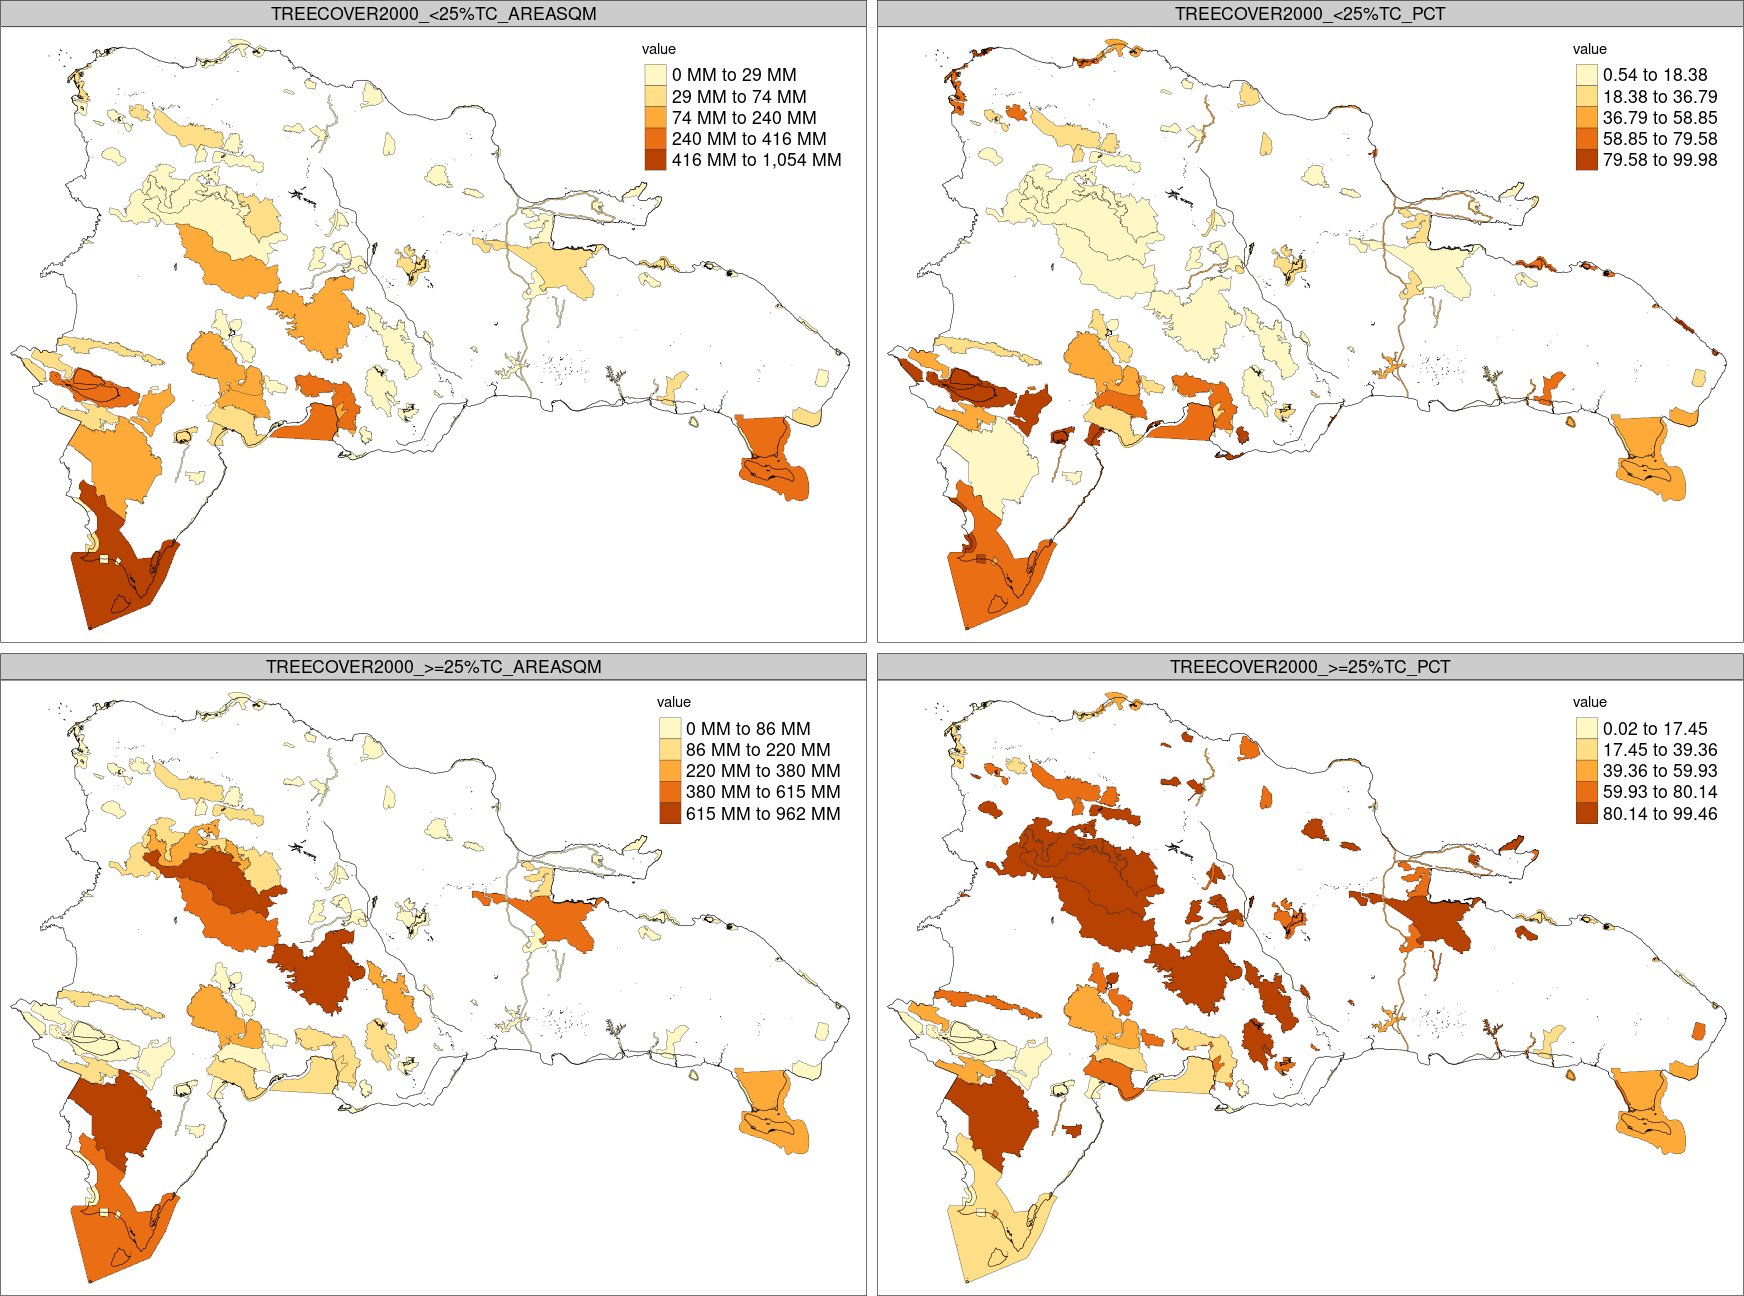
\includegraphics{img/data-download-preparation-eda/zonal-pa-1} \end{center}

\begin{Shaded}
\begin{Highlighting}[]
\CommentTok{\# Top twenty sorted descending by column 2}
\FunctionTok{stripped\_table}\NormalTok{(pazonal }\SpecialCharTok{\%\textgreater{}\%} \FunctionTok{select}\NormalTok{(CATEGORY\_NAME, }\FunctionTok{matches}\NormalTok{(}\StringTok{\textquotesingle{}\^{}TREECOVER2000\textquotesingle{}}\NormalTok{)))}
\end{Highlighting}
\end{Shaded}

\begin{table}[H]
\centering
\begin{tabular}[t]{llrrrr}
\toprule
  & CATEGORY\_NAME & TREECOVER2000\_>=25\%TC\_PCT & TREECOVER2000\_<25\%TC\_PCT & TREECOVER2000\_>=25\%TC\_AREASQM & TREECOVER2000\_<25\%TC\_AREASQM\\
\midrule
\cellcolor{lightgray}{1} & \cellcolor{lightgray}{Reserva Cientifica Ébano Verde} & \cellcolor{lightgray}{99.45886} & \cellcolor{lightgray}{0.5411389} & \cellcolor{lightgray}{29737413} & \cellcolor{lightgray}{161796.2}\\
2 & Parque Nacional Armando Bermúdez & 99.44928 & 0.5507213 & 798130271 & 4419814.0\\
\cellcolor{lightgray}{3} & \cellcolor{lightgray}{Reserva Biológica Sierra Prieta} & \cellcolor{lightgray}{96.83358} & \cellcolor{lightgray}{3.1664212} & \cellcolor{lightgray}{3873387} & \cellcolor{lightgray}{126658.3}\\
4 & Monumento Natural Salto de Jimenoa & 96.73826 & 3.2617410 & 16862472 & 568555.0\\
\cellcolor{lightgray}{5} & \cellcolor{lightgray}{Monumento Natural Salto de La Damajagua} & \cellcolor{lightgray}{96.29039} & \cellcolor{lightgray}{3.7096131} & \cellcolor{lightgray}{5320742} & \cellcolor{lightgray}{204983.0}\\
\addlinespace
6 & Reserva Cientifica Loma Barbacoa & 95.98497 & 4.0150295 & 13157487 & 550374.7\\
\cellcolor{lightgray}{7} & \cellcolor{lightgray}{Reserva Cientifica Loma Guaconejo} & \cellcolor{lightgray}{95.74294} & \cellcolor{lightgray}{4.2570610} & \cellcolor{lightgray}{22376360} & \cellcolor{lightgray}{994930.1}\\
8 & Area Nacional De Recreo Guagui & 95.15097 & 4.8490329 & 39462770 & 2011080.6\\
\cellcolor{lightgray}{9} & \cellcolor{lightgray}{Monumento Natural Loma Isabel de Torres} & \cellcolor{lightgray}{94.52917} & \cellcolor{lightgray}{5.4708282} & \cellcolor{lightgray}{15696490} & \cellcolor{lightgray}{908426.4}\\
10 & Parque Nacional Los Haitises & 94.36072 & 5.6392834 & 596059009 & 35622299.1\\
\addlinespace
\cellcolor{lightgray}{11} & \cellcolor{lightgray}{Parque Nacional Montaña La Humeadora} & \cellcolor{lightgray}{94.02525} & \cellcolor{lightgray}{5.9747549} & \cellcolor{lightgray}{287161000} & \cellcolor{lightgray}{18247403.6}\\
12 & Reserva Cientifica Las Neblinas & 93.37844 & 6.6215607 & 38076127 & 2700017.1\\
\cellcolor{lightgray}{13} & \cellcolor{lightgray}{Reserva Forestal Loma Novillero} & \cellcolor{lightgray}{93.31888} & \cellcolor{lightgray}{6.6811206} & \cellcolor{lightgray}{12028318} & \cellcolor{lightgray}{861161.7}\\
14 & Parque Nacional Manolo Tavarez Justo & 93.04410 & 6.9558961 & 327260774 & 24465730.1\\
\cellcolor{lightgray}{15} & \cellcolor{lightgray}{Monumento Natural Diego de Ocampo} & \cellcolor{lightgray}{92.85590} & \cellcolor{lightgray}{7.1441013} & \cellcolor{lightgray}{23532983} & \cellcolor{lightgray}{1810569.0}\\
\addlinespace
16 & Reserva Cientifica Loma Quita Espuela & 92.70482 & 7.2951783 & 70211435 & 5525116.5\\
\cellcolor{lightgray}{17} & \cellcolor{lightgray}{Parque Nacional Picky Lora} & \cellcolor{lightgray}{92.31943} & \cellcolor{lightgray}{7.6805670} & \cellcolor{lightgray}{103652897} & \cellcolor{lightgray}{8623460.9}\\
18 & Monumento Natural Cerro de San Francisco & 90.71807 & 9.2819295 & 3651148 & 373571.7\\
\cellcolor{lightgray}{19} & \cellcolor{lightgray}{Reserva Forestal Alto Mao} & \cellcolor{lightgray}{89.03664} & \cellcolor{lightgray}{10.9633598} & \cellcolor{lightgray}{187078973} & \cellcolor{lightgray}{23035618.6}\\
20 & Parque Nacional Saltos de la Jalda & 88.18683 & 11.8131702 & 32129714 & 4303973.5\\
\bottomrule
\end{tabular}
\end{table}

\begin{Shaded}
\begin{Highlighting}[]
\CommentTok{\# ALL sorted descending by column 2}
\FunctionTok{stripped\_table}\NormalTok{(}
\NormalTok{  pazonal }\SpecialCharTok{\%\textgreater{}\%} \FunctionTok{select}\NormalTok{(CATEGORY\_NAME, }\FunctionTok{matches}\NormalTok{(}\StringTok{\textquotesingle{}\^{}TREECOVER2000\textquotesingle{}}\NormalTok{)) }\SpecialCharTok{\%\textgreater{}\%} \FunctionTok{select}\NormalTok{(}\SpecialCharTok{{-}}\FunctionTok{matches}\NormalTok{(}\StringTok{\textquotesingle{}\textless{}NA\textgreater{}\textquotesingle{}}\NormalTok{)),}
  \AttributeTok{order\_col =} \DecValTok{1}\NormalTok{, }\AttributeTok{n =} \FunctionTok{nrow}\NormalTok{(pazonal),}
  \AttributeTok{long\_table =}\NormalTok{ T}
\NormalTok{)}
\end{Highlighting}
\end{Shaded}

\begin{longtable}[t]{llrrrr}
\toprule
  & CATEGORY\_NAME & TREECOVER2000\_>=25\%TC\_PCT & TREECOVER2000\_<25\%TC\_PCT & TREECOVER2000\_>=25\%TC\_AREASQM & TREECOVER2000\_<25\%TC\_AREASQM\\
\midrule
\endfirsthead
\multicolumn{6}{@{}l}{\textit{(continued)}}\\
\toprule
  & CATEGORY\_NAME & TREECOVER2000\_>=25\%TC\_PCT & TREECOVER2000\_<25\%TC\_PCT & TREECOVER2000\_>=25\%TC\_AREASQM & TREECOVER2000\_<25\%TC\_AREASQM\\
\midrule
\endhead

\endfoot
\bottomrule
\endlastfoot
\cellcolor{lightgray}{1} & \cellcolor{lightgray}{Via Panoramica Vía Panorámica Costa Azul} & \cellcolor{lightgray}{16.3307853} & \cellcolor{lightgray}{83.6692147} & \cellcolor{lightgray}{3.112644e+06} & \cellcolor{lightgray}{15947334.9}\\
2 & Via Panoramica Mirador del Paraíso & 39.3640466 & 60.6359534 & 8.275303e+06 & 12747187.0\\
\cellcolor{lightgray}{3} & \cellcolor{lightgray}{Via Panoramica Mirador del Atlántico} & \cellcolor{lightgray}{51.3662861} & \cellcolor{lightgray}{48.6337139} & \cellcolor{lightgray}{6.223541e+06} & \cellcolor{lightgray}{5892462.7}\\
4 & Via Panoramica Entrada de Mao & 71.5352663 & 28.4647337 & 3.889122e+07 & 15475281.1\\
\cellcolor{lightgray}{5} & \cellcolor{lightgray}{Via Panoramica Carretera Santiago - La Cumbre - Puerto Plata} & \cellcolor{lightgray}{59.2508235} & \cellcolor{lightgray}{40.7491765} & \cellcolor{lightgray}{1.243086e+07} & \cellcolor{lightgray}{8549200.8}\\
\addlinespace
6 & Via Panoramica Carretera Nagua - Sánchez & 58.0140667 & 41.9859333 & 9.773630e+06 & 7073370.0\\
\cellcolor{lightgray}{7} & \cellcolor{lightgray}{Via Panoramica Carretera El Abanico - Constanza} & \cellcolor{lightgray}{57.6227891} & \cellcolor{lightgray}{42.3772109} & \cellcolor{lightgray}{1.310670e+07} & \cellcolor{lightgray}{9638986.5}\\
8 & Via Panoramica Carretera Cabral - Polo & 59.9304146 & 40.0695854 & 6.089977e+06 & 4071769.9\\
\cellcolor{lightgray}{9} & \cellcolor{lightgray}{Via Panoramica Carretera Bayacanes-Jarabacoa} & \cellcolor{lightgray}{73.7080689} & \cellcolor{lightgray}{26.2919311} & \cellcolor{lightgray}{1.196090e+07} & \cellcolor{lightgray}{4266496.6}\\
10 & Via Panoramica Autovia Santo Domingo - Samana - Boulevar del Atlantico & 57.7894782 & 42.2105218 & 5.969193e+07 & 43600110.1\\
\addlinespace
\cellcolor{lightgray}{11} & \cellcolor{lightgray}{Santuario De Mamiferos Marinos Estero Hondo} & \cellcolor{lightgray}{31.2148392} & \cellcolor{lightgray}{68.7851608} & \cellcolor{lightgray}{1.015811e+07} & \cellcolor{lightgray}{22384455.7}\\
12 & Reserva Forestal Villarpando & 79.6642464 & 20.3357536 & 6.337343e+07 & 16177225.7\\
\cellcolor{lightgray}{13} & \cellcolor{lightgray}{Reserva Forestal Río Cana} & \cellcolor{lightgray}{80.1427532} & \cellcolor{lightgray}{19.8572468} & \cellcolor{lightgray}{2.083290e+08} & \cellcolor{lightgray}{51618405.8}\\
14 & Reserva Forestal Loma Novillero & 93.3188794 & 6.6811206 & 1.202832e+07 & 861161.7\\
\cellcolor{lightgray}{15} & \cellcolor{lightgray}{Reserva Forestal Loma El 20} & \cellcolor{lightgray}{69.5133433} & \cellcolor{lightgray}{30.4866567} & \cellcolor{lightgray}{3.476835e+07} & \cellcolor{lightgray}{15248448.2}\\
\addlinespace
16 & Reserva Forestal Las Matas & 20.9660036 & 79.0339964 & 1.001703e+07 & 37760440.8\\
\cellcolor{lightgray}{17} & \cellcolor{lightgray}{Reserva Forestal Hatillo} & \cellcolor{lightgray}{63.6135031} & \cellcolor{lightgray}{36.3864969} & \cellcolor{lightgray}{2.030413e+08} & \cellcolor{lightgray}{116138281.8}\\
18 & Reserva Forestal Guanito & 70.9588252 & 29.0411748 & 4.892286e+07 & 20022561.6\\
\cellcolor{lightgray}{19} & \cellcolor{lightgray}{Reserva Forestal Cerro de Bocanigua} & \cellcolor{lightgray}{8.6179107} & \cellcolor{lightgray}{91.3820893} & \cellcolor{lightgray}{2.517152e+06} & \cellcolor{lightgray}{26691226.5}\\
20 & Reserva Forestal Cerro Chacuey & 84.8994811 & 15.1005189 & 4.405685e+07 & 7836105.6\\
\addlinespace
\cellcolor{lightgray}{21} & \cellcolor{lightgray}{Reserva Forestal Cayuco} & \cellcolor{lightgray}{88.0875912} & \cellcolor{lightgray}{11.9124088} & \cellcolor{lightgray}{4.438683e+06} & \cellcolor{lightgray}{600259.4}\\
22 & Reserva Forestal Cabeza de Toro & 70.1046838 & 29.8953162 & 2.633262e+08 & 112292355.2\\
\cellcolor{lightgray}{23} & \cellcolor{lightgray}{Reserva Forestal Barrero} & \cellcolor{lightgray}{26.1405649} & \cellcolor{lightgray}{73.8594351} & \cellcolor{lightgray}{8.120355e+07} & \cellcolor{lightgray}{229438349.3}\\
24 & Reserva Forestal Arroyo Cano & 84.4863667 & 15.5136333 & 2.019122e+07 & 3707571.4\\
\cellcolor{lightgray}{25} & \cellcolor{lightgray}{Reserva Forestal Alto Mao} & \cellcolor{lightgray}{89.0366402} & \cellcolor{lightgray}{10.9633598} & \cellcolor{lightgray}{1.870790e+08} & \cellcolor{lightgray}{23035618.6}\\
\addlinespace
26 & Reserva Forestal Alto bao & 83.9546228 & 16.0453772 & 2.204493e+08 & 42132192.7\\
\cellcolor{lightgray}{27} & \cellcolor{lightgray}{Reserva Cientifica Loma Quita Espuela} & \cellcolor{lightgray}{92.7048217} & \cellcolor{lightgray}{7.2951783} & \cellcolor{lightgray}{7.021144e+07} & \cellcolor{lightgray}{5525116.5}\\
28 & Reserva Cientifica Loma Guaconejo & 95.7429390 & 4.2570610 & 2.237636e+07 & 994930.1\\
\cellcolor{lightgray}{29} & \cellcolor{lightgray}{Reserva Cientifica Loma Barbacoa} & \cellcolor{lightgray}{95.9849705} & \cellcolor{lightgray}{4.0150295} & \cellcolor{lightgray}{1.315749e+07} & \cellcolor{lightgray}{550374.7}\\
30 & Reserva Cientifica Las Neblinas & 93.3784393 & 6.6215607 & 3.807613e+07 & 2700017.1\\
\addlinespace
\cellcolor{lightgray}{31} & \cellcolor{lightgray}{Reserva Cientifica La Salcedoa} & \cellcolor{lightgray}{77.5760173} & \cellcolor{lightgray}{22.4239827} & \cellcolor{lightgray}{3.197405e+07} & \cellcolor{lightgray}{9242360.9}\\
32 & Reserva Cientifica Ébano Verde & 99.4588611 & 0.5411389 & 2.973741e+07 & 161796.2\\
\cellcolor{lightgray}{33} & \cellcolor{lightgray}{Reserva Biológica Sierra Prieta} & \cellcolor{lightgray}{96.8335788} & \cellcolor{lightgray}{3.1664212} & \cellcolor{lightgray}{3.873387e+06} & \cellcolor{lightgray}{126658.3}\\
34 & Reserva Biológica Loma Charco Azul & 57.3430148 & 42.6569852 & 9.988543e+07 & 74303929.7\\
\cellcolor{lightgray}{35} & \cellcolor{lightgray}{Refugio de Vida Silvestre Río Soco} & \cellcolor{lightgray}{45.1802336} & \cellcolor{lightgray}{54.8197664} & \cellcolor{lightgray}{5.315016e+06} & \cellcolor{lightgray}{6449013.7}\\
\addlinespace
36 & Refugio de Vida Silvestre Río Higuamo & 65.8064260 & 34.1935740 & 1.216933e+07 & 6323287.4\\
\cellcolor{lightgray}{37} & \cellcolor{lightgray}{Refugio de Vida Silvestre Río Chacuey} & \cellcolor{lightgray}{77.3000664} & \cellcolor{lightgray}{22.6999336} & \cellcolor{lightgray}{2.997265e+07} & \cellcolor{lightgray}{8801768.0}\\
38 & Refugio de Vida Silvestre Ría Maimón & 49.8247218 & 50.1752782 & 2.405438e+06 & 2422362.4\\
\cellcolor{lightgray}{39} & \cellcolor{lightgray}{Refugio de Vida Silvestre Monumento Natural Miguel Domingo Fuerte} & \cellcolor{lightgray}{84.0686221} & \cellcolor{lightgray}{15.9313779} & \cellcolor{lightgray}{2.818711e+07} & \cellcolor{lightgray}{5341582.1}\\
40 & Refugio de Vida Silvestre Manglares de Puerto Viejo & 7.8763050 & 92.1236950 & 8.769266e+05 & 10256804.7\\
\addlinespace
\cellcolor{lightgray}{41} & \cellcolor{lightgray}{Refugio de Vida Silvestre Manglar de la Jina} & \cellcolor{lightgray}{24.9558113} & \cellcolor{lightgray}{75.0441887} & \cellcolor{lightgray}{1.319275e+07} & \cellcolor{lightgray}{39671701.7}\\
42 & Refugio de Vida Silvestre Lagunas Redonda y Limón & 36.1311239 & 63.8688761 & 9.594479e+06 & 16960131.6\\
\cellcolor{lightgray}{43} & \cellcolor{lightgray}{Refugio de Vida Silvestre Lagunas de Bávaro y El Caletón} & \cellcolor{lightgray}{20.4231831} & \cellcolor{lightgray}{79.5768169} & \cellcolor{lightgray}{1.307073e+06} & \cellcolor{lightgray}{5092873.7}\\
44 & Refugio de Vida Silvestre Laguna Saladilla & 30.4988180 & 69.5011820 & 9.489458e+06 & 21624725.7\\
\cellcolor{lightgray}{45} & \cellcolor{lightgray}{Refugio de Vida Silvestre Laguna Cabral o Rincón} & \cellcolor{lightgray}{4.0765686} & \cellcolor{lightgray}{95.9234314} & \cellcolor{lightgray}{2.284298e+06} & \cellcolor{lightgray}{53750526.7}\\
\addlinespace
46 & Refugio de Vida Silvestre La Gran Laguna o Perucho & 33.8233813 & 66.1766187 & 2.475744e+06 & 4843880.0\\
\cellcolor{lightgray}{47} & \cellcolor{lightgray}{Refugio de Vida Silvestre Humedales del Bajo Yaque del Sur} & \cellcolor{lightgray}{3.8745155} & \cellcolor{lightgray}{96.1254845} & \cellcolor{lightgray}{2.265132e+06} & \cellcolor{lightgray}{56197194.2}\\
48 & Refugio de Vida Silvestre Cañón Río Gurabo & 74.8286878 & 25.1713122 & 2.256819e+07 & 7591620.2\\
\cellcolor{lightgray}{49} & \cellcolor{lightgray}{Refugio de Vida Silvestre Bahia de Luperón} & \cellcolor{lightgray}{43.6916900} & \cellcolor{lightgray}{56.3083100} & \cellcolor{lightgray}{8.163662e+06} & \cellcolor{lightgray}{10521039.6}\\
50 & Parque Nacional Valle Nuevo & 84.5282712 & 15.4717288 & 7.659372e+08 & 140194190.1\\
\addlinespace
\cellcolor{lightgray}{51} & \cellcolor{lightgray}{Parque Nacional Sierra Martín García} & \cellcolor{lightgray}{72.8168067} & \cellcolor{lightgray}{27.1831933} & \cellcolor{lightgray}{1.904179e+08} & \cellcolor{lightgray}{71084794.4}\\
52 & Parque Nacional Sierra de Neiba & 69.6271339 & 30.3728661 & 1.274175e+08 & 55582293.7\\
\cellcolor{lightgray}{53} & \cellcolor{lightgray}{Parque Nacional Sierra de Bahoruco} & \cellcolor{lightgray}{88.1011026} & \cellcolor{lightgray}{11.8988974} & \cellcolor{lightgray}{9.623023e+08} & \cellcolor{lightgray}{129968135.2}\\
54 & Parque Nacional Saltos de la Jalda & 88.1868298 & 11.8131702 & 3.212971e+07 & 4303973.5\\
\cellcolor{lightgray}{55} & \cellcolor{lightgray}{Parque Nacional Punta Espada} & \cellcolor{lightgray}{49.9096730} & \cellcolor{lightgray}{50.0903270} & \cellcolor{lightgray}{4.104462e+07} & \cellcolor{lightgray}{41193188.6}\\
\addlinespace
56 & Parque Nacional Picky Lora & 92.3194330 & 7.6805670 & 1.036529e+08 & 8623460.9\\
\cellcolor{lightgray}{57} & \cellcolor{lightgray}{Parque Nacional Nalga de Maco} & \cellcolor{lightgray}{82.6462447} & \cellcolor{lightgray}{17.3537553} & \cellcolor{lightgray}{1.370679e+08} & \cellcolor{lightgray}{28781005.0}\\
58 & Parque Nacional Montaña La Humeadora & 94.0252451 & 5.9747549 & 2.871610e+08 & 18247403.6\\
\cellcolor{lightgray}{59} & \cellcolor{lightgray}{Parque Nacional Máximo Gómez} & \cellcolor{lightgray}{76.1949505} & \cellcolor{lightgray}{23.8050495} & \cellcolor{lightgray}{3.222647e+07} & \cellcolor{lightgray}{10068289.4}\\
60 & Parque Nacional Manolo Tavarez Justo & 93.0441039 & 6.9558961 & 3.272608e+08 & 24465730.1\\
\addlinespace
\cellcolor{lightgray}{61} & \cellcolor{lightgray}{Parque Nacional Manglares del Bajo Yuna} & \cellcolor{lightgray}{78.3065153} & \cellcolor{lightgray}{21.6934847} & \cellcolor{lightgray}{9.487214e+07} & \cellcolor{lightgray}{26282708.9}\\
62 & Parque Nacional Manglares de Estero Balsa & 33.3944954 & 66.6055046 & 1.888339e+07 & 37663017.7\\
\cellcolor{lightgray}{63} & \cellcolor{lightgray}{Parque Nacional Luis Quin} & \cellcolor{lightgray}{86.8040330} & \cellcolor{lightgray}{13.1959670} & \cellcolor{lightgray}{1.712595e+08} & \cellcolor{lightgray}{26034908.2}\\
64 & Parque Nacional Los Haitises & 94.3607166 & 5.6392834 & 5.960590e+08 & 35622299.1\\
\cellcolor{lightgray}{65} & \cellcolor{lightgray}{Parque Nacional Lago Enriquillo e Isla Cabritos} & \cellcolor{lightgray}{1.6547394} & \cellcolor{lightgray}{98.3452606} & \cellcolor{lightgray}{6.700602e+06} & \cellcolor{lightgray}{398233395.5}\\
\addlinespace
66 & Parque Nacional La Hispaniola & 50.0098947 & 49.9901053 & 2.741823e+07 & 27407377.2\\
\cellcolor{lightgray}{67} & \cellcolor{lightgray}{Parque Nacional La Gran Sabana} & \cellcolor{lightgray}{6.7321418} & \cellcolor{lightgray}{93.2678582} & \cellcolor{lightgray}{1.478217e+07} & \cellcolor{lightgray}{204793812.2}\\
68 & Parque Nacional José del Carmen Ramírez & 82.0178580 & 17.9821420 & 6.149357e+08 & 134822601.0\\
\cellcolor{lightgray}{69} & \cellcolor{lightgray}{Parque Nacional Jaragua} & \cellcolor{lightgray}{31.3660689} & \cellcolor{lightgray}{68.6339311} & \cellcolor{lightgray}{4.814738e+08} & \cellcolor{lightgray}{1053541025.4}\\
70 & Parque Nacional Humedales del Ozama & 43.4198647 & 56.5801353 & 2.015476e+07 & 26263538.8\\
\addlinespace
\cellcolor{lightgray}{71} & \cellcolor{lightgray}{Parque Nacional Francisco Alberto Caamaño Deñó} & \cellcolor{lightgray}{33.6662104} & \cellcolor{lightgray}{66.3337896} & \cellcolor{lightgray}{1.977924e+08} & \cellcolor{lightgray}{389717643.3}\\
72 & Parque Nacional El Morro & 17.4540788 & 82.5459212 & 3.205114e+06 & 15158008.2\\
\cellcolor{lightgray}{73} & \cellcolor{lightgray}{Parque Nacional Cotubanamá (Del Este)} & \cellcolor{lightgray}{47.7556133} & \cellcolor{lightgray}{52.2443867} & \cellcolor{lightgray}{3.803282e+08} & \cellcolor{lightgray}{416077050.5}\\
74 & Parque Nacional Cabo Cabrón & 87.4517255 & 12.5482745 & 3.115334e+07 & 4470131.5\\
\cellcolor{lightgray}{75} & \cellcolor{lightgray}{Parque Nacional Baiguate} & \cellcolor{lightgray}{86.6759322} & \cellcolor{lightgray}{13.3240678} & \cellcolor{lightgray}{4.544164e+07} & \cellcolor{lightgray}{6985416.1}\\
\addlinespace
76 & Parque Nacional Armando Bermúdez & 99.4492787 & 0.5507213 & 7.981303e+08 & 4419814.0\\
\cellcolor{lightgray}{77} & \cellcolor{lightgray}{Parque Nacional Aniana Vargas} & \cellcolor{lightgray}{66.2654500} & \cellcolor{lightgray}{33.7345500} & \cellcolor{lightgray}{8.589790e+07} & \cellcolor{lightgray}{43729077.2}\\
78 & Parque Nacional Anacaona & 55.3803711 & 44.6196289 & 2.984618e+08 & 240468883.3\\
\cellcolor{lightgray}{79} & \cellcolor{lightgray}{Monumento Natural Saltos de Jima} & \cellcolor{lightgray}{64.1597654} & \cellcolor{lightgray}{35.8402346} & \cellcolor{lightgray}{1.191080e+07} & \cellcolor{lightgray}{6653483.8}\\
80 & Monumento Natural Salto Grande & 72.4481659 & 27.5518341 & 1.069278e+07 & 4066434.4\\
\addlinespace
\cellcolor{lightgray}{81} & \cellcolor{lightgray}{Monumento Natural Salto El Limón} & \cellcolor{lightgray}{88.1772739} & \cellcolor{lightgray}{11.8227261} & \cellcolor{lightgray}{1.452719e+07} & \cellcolor{lightgray}{1947792.3}\\
82 & Monumento Natural Salto de Socoa & 77.9952416 & 22.0047584 & 5.327307e+07 & 15029904.4\\
\cellcolor{lightgray}{83} & \cellcolor{lightgray}{Monumento Natural Salto de La Damajagua} & \cellcolor{lightgray}{96.2903869} & \cellcolor{lightgray}{3.7096131} & \cellcolor{lightgray}{5.320742e+06} & \cellcolor{lightgray}{204983.0}\\
84 & Monumento Natural Salto de Jimenoa & 96.7382590 & 3.2617410 & 1.686247e+07 & 568555.0\\
\cellcolor{lightgray}{85} & \cellcolor{lightgray}{Monumento Natural Río Cumayasa y Cueva de las Maravillas} & \cellcolor{lightgray}{36.6842668} & \cellcolor{lightgray}{63.3157332} & \cellcolor{lightgray}{3.256086e+07} & \cellcolor{lightgray}{56198878.1}\\
\addlinespace
86 & Monumento Natural Reserva Antropológica Cuevas de Borbón o del Pomier & 63.2103105 & 36.7896895 & 3.174434e+06 & 1847585.3\\
\cellcolor{lightgray}{87} & \cellcolor{lightgray}{Monumento Natural Los Cacheos} & \cellcolor{lightgray}{0.8271550} & \cellcolor{lightgray}{99.1728450} & \cellcolor{lightgray}{4.613026e+05} & \cellcolor{lightgray}{55308489.8}\\
88 & Monumento Natural Loma Isabel de Torres & 94.5291718 & 5.4708282 & 1.569649e+07 & 908426.4\\
\cellcolor{lightgray}{89} & \cellcolor{lightgray}{Monumento Natural Las Marías} & \cellcolor{lightgray}{27.0243743} & \cellcolor{lightgray}{72.9756257} & \cellcolor{lightgray}{1.217374e+06} & \cellcolor{lightgray}{3287352.9}\\
90 & Monumento Natural Las Dunas de las Calderas & 16.9268970 & 83.0731030 & 2.958687e+06 & 14520516.3\\
\addlinespace
\cellcolor{lightgray}{91} & \cellcolor{lightgray}{Monumento Natural Las Caobas} & \cellcolor{lightgray}{53.9809062} & \cellcolor{lightgray}{46.0190938} & \cellcolor{lightgray}{5.693486e+07} & \cellcolor{lightgray}{48537361.9}\\
92 & Monumento Natural Lagunas Cabarete y Goleta & 74.2833726 & 25.7166274 & 5.333655e+07 & 18464916.9\\
\cellcolor{lightgray}{93} & \cellcolor{lightgray}{Monumento Natural La Tinaja} & \cellcolor{lightgray}{81.6231436} & \cellcolor{lightgray}{18.3768564} & \cellcolor{lightgray}{2.409466e+07} & \cellcolor{lightgray}{5424736.3}\\
94 & Monumento Natural Isla Catalina & 48.2635273 & 51.7364727 & 7.837690e+06 & 8401674.6\\
\cellcolor{lightgray}{95} & \cellcolor{lightgray}{Monumento Natural Hoyo Claro} & \cellcolor{lightgray}{67.0247609} & \cellcolor{lightgray}{32.9752391} & \cellcolor{lightgray}{2.633797e+07} & \cellcolor{lightgray}{12957912.7}\\
\addlinespace
96 & Monumento Natural Diego de Ocampo & 92.8558987 & 7.1441013 & 2.353298e+07 & 1810569.0\\
\cellcolor{lightgray}{97} & \cellcolor{lightgray}{Monumento Natural Cerro de San Francisco} & \cellcolor{lightgray}{90.7180705} & \cellcolor{lightgray}{9.2819295} & \cellcolor{lightgray}{3.651148e+06} & \cellcolor{lightgray}{373571.7}\\
98 & Monumento Natural Cabo Samaná & 79.2496232 & 20.7503768 & 7.346906e+06 & 1923682.0\\
\cellcolor{lightgray}{99} & \cellcolor{lightgray}{Corredor Ecologico Autopista Juan Bosch} & \cellcolor{lightgray}{22.1218962} & \cellcolor{lightgray}{77.8781038} & \cellcolor{lightgray}{1.227294e+06} & \cellcolor{lightgray}{4320574.7}\\
100 & Corredor Ecologico Autopista Duarte & 41.1485625 & 58.8514375 & 4.265560e+06 & 6100682.9\\
\addlinespace
\cellcolor{lightgray}{101} & \cellcolor{lightgray}{Corredor Ecologico Autopista 6 de Noviembre} & \cellcolor{lightgray}{20.5983424} & \cellcolor{lightgray}{79.4016576} & \cellcolor{lightgray}{7.483224e+05} & \cellcolor{lightgray}{2884602.8}\\
102 & Area Nacional De Recreo Playa Larga & 0.0197443 & 99.9802557 & 2.961669e+03 & 14997150.5\\
\cellcolor{lightgray}{103} & \cellcolor{lightgray}{Area Nacional De Recreo Playa de Cabo Rojo - Pedernales} & \cellcolor{lightgray}{6.7464316} & \cellcolor{lightgray}{93.2535684} & \cellcolor{lightgray}{1.181795e+06} & \cellcolor{lightgray}{16335533.9}\\
104 & Area Nacional De Recreo Playa Blanca & 51.8436741 & 48.1563259 & 3.454111e+06 & 3208439.2\\
\cellcolor{lightgray}{105} & \cellcolor{lightgray}{Area Nacional De Recreo Guaraguao - Punta Catuano} & \cellcolor{lightgray}{67.2725113} & \cellcolor{lightgray}{32.7274887} & \cellcolor{lightgray}{1.250931e+07} & \cellcolor{lightgray}{6085669.8}\\
\addlinespace
106 & Area Nacional De Recreo Guagui & 95.1509671 & 4.8490329 & 3.946277e+07 & 2011080.6\\
\cellcolor{lightgray}{107} & \cellcolor{lightgray}{Area Nacional De Recreo Boca de Nigua} & \cellcolor{lightgray}{15.0601647} & \cellcolor{lightgray}{84.9398353} & \cellcolor{lightgray}{8.757018e+05} & \cellcolor{lightgray}{4938987.4}\\
108 & Area Nacional De Recreo Bahía de las Águilas & 1.1695259 & 98.8304741 & 4.665196e+05 & 39423115.7\\*
\end{longtable}

\begin{Shaded}
\begin{Highlighting}[]

\CommentTok{\# Loss year}
\CommentTok{\# * PCT}
\NormalTok{pazonal }\SpecialCharTok{\%\textgreater{}\%} \FunctionTok{select}\NormalTok{(}\FunctionTok{matches}\NormalTok{(}\StringTok{\textquotesingle{}\^{}LOSSYEAR\_[1{-}9].*\_PCT$\textquotesingle{}}\NormalTok{)) }\SpecialCharTok{\%\textgreater{}\%}
  \FunctionTok{gather}\NormalTok{(variable, value, }\SpecialCharTok{{-}}\NormalTok{geom) }\SpecialCharTok{\%\textgreater{}\%}
  \FunctionTok{mutate}\NormalTok{(}\AttributeTok{variable =} \FunctionTok{factor}\NormalTok{(variable, }\AttributeTok{levels =} \FunctionTok{unique}\NormalTok{(variable))) }\SpecialCharTok{\%\textgreater{}\%} 
  \FunctionTok{tm\_shape}\NormalTok{() }\SpecialCharTok{+}
  \FunctionTok{tm\_fill}\NormalTok{(}\AttributeTok{col=}\StringTok{\textquotesingle{}value\textquotesingle{}}\NormalTok{, }\AttributeTok{palette =} \StringTok{"YlOrBr"}\NormalTok{, }\AttributeTok{size =} \FloatTok{0.1}\NormalTok{, }\AttributeTok{style =} \StringTok{\textquotesingle{}jenks\textquotesingle{}}\NormalTok{) }\SpecialCharTok{+}
  \FunctionTok{tm\_borders}\NormalTok{(}\AttributeTok{col =} \StringTok{\textquotesingle{}grey15\textquotesingle{}}\NormalTok{, }\AttributeTok{lwd =} \FloatTok{0.3}\NormalTok{) }\SpecialCharTok{+}
  \FunctionTok{tm\_facets}\NormalTok{(}\AttributeTok{by =} \StringTok{"variable"}\NormalTok{, }\AttributeTok{ncol =} \DecValTok{5}\NormalTok{, }\AttributeTok{nrow =} \DecValTok{4}\NormalTok{, }\AttributeTok{free.coords =} \ConstantTok{FALSE}\NormalTok{, }\AttributeTok{free.scales =} \ConstantTok{TRUE}\NormalTok{) }\SpecialCharTok{+}
  \FunctionTok{tm\_layout}\NormalTok{(}\AttributeTok{panel.label.size =} \DecValTok{1}\NormalTok{, }\AttributeTok{legend.title.size =} \DecValTok{1}\NormalTok{, }\AttributeTok{legend.text.size =} \FloatTok{0.75}\NormalTok{) }\SpecialCharTok{+} 
  \FunctionTok{tm\_shape}\NormalTok{(}\AttributeTok{shp =}\NormalTok{ cline) }\SpecialCharTok{+} \FunctionTok{tm\_borders}\NormalTok{(}\AttributeTok{col =} \StringTok{\textquotesingle{}black\textquotesingle{}}\NormalTok{, }\AttributeTok{lwd =} \FloatTok{0.5}\NormalTok{)}
\end{Highlighting}
\end{Shaded}

\begin{center}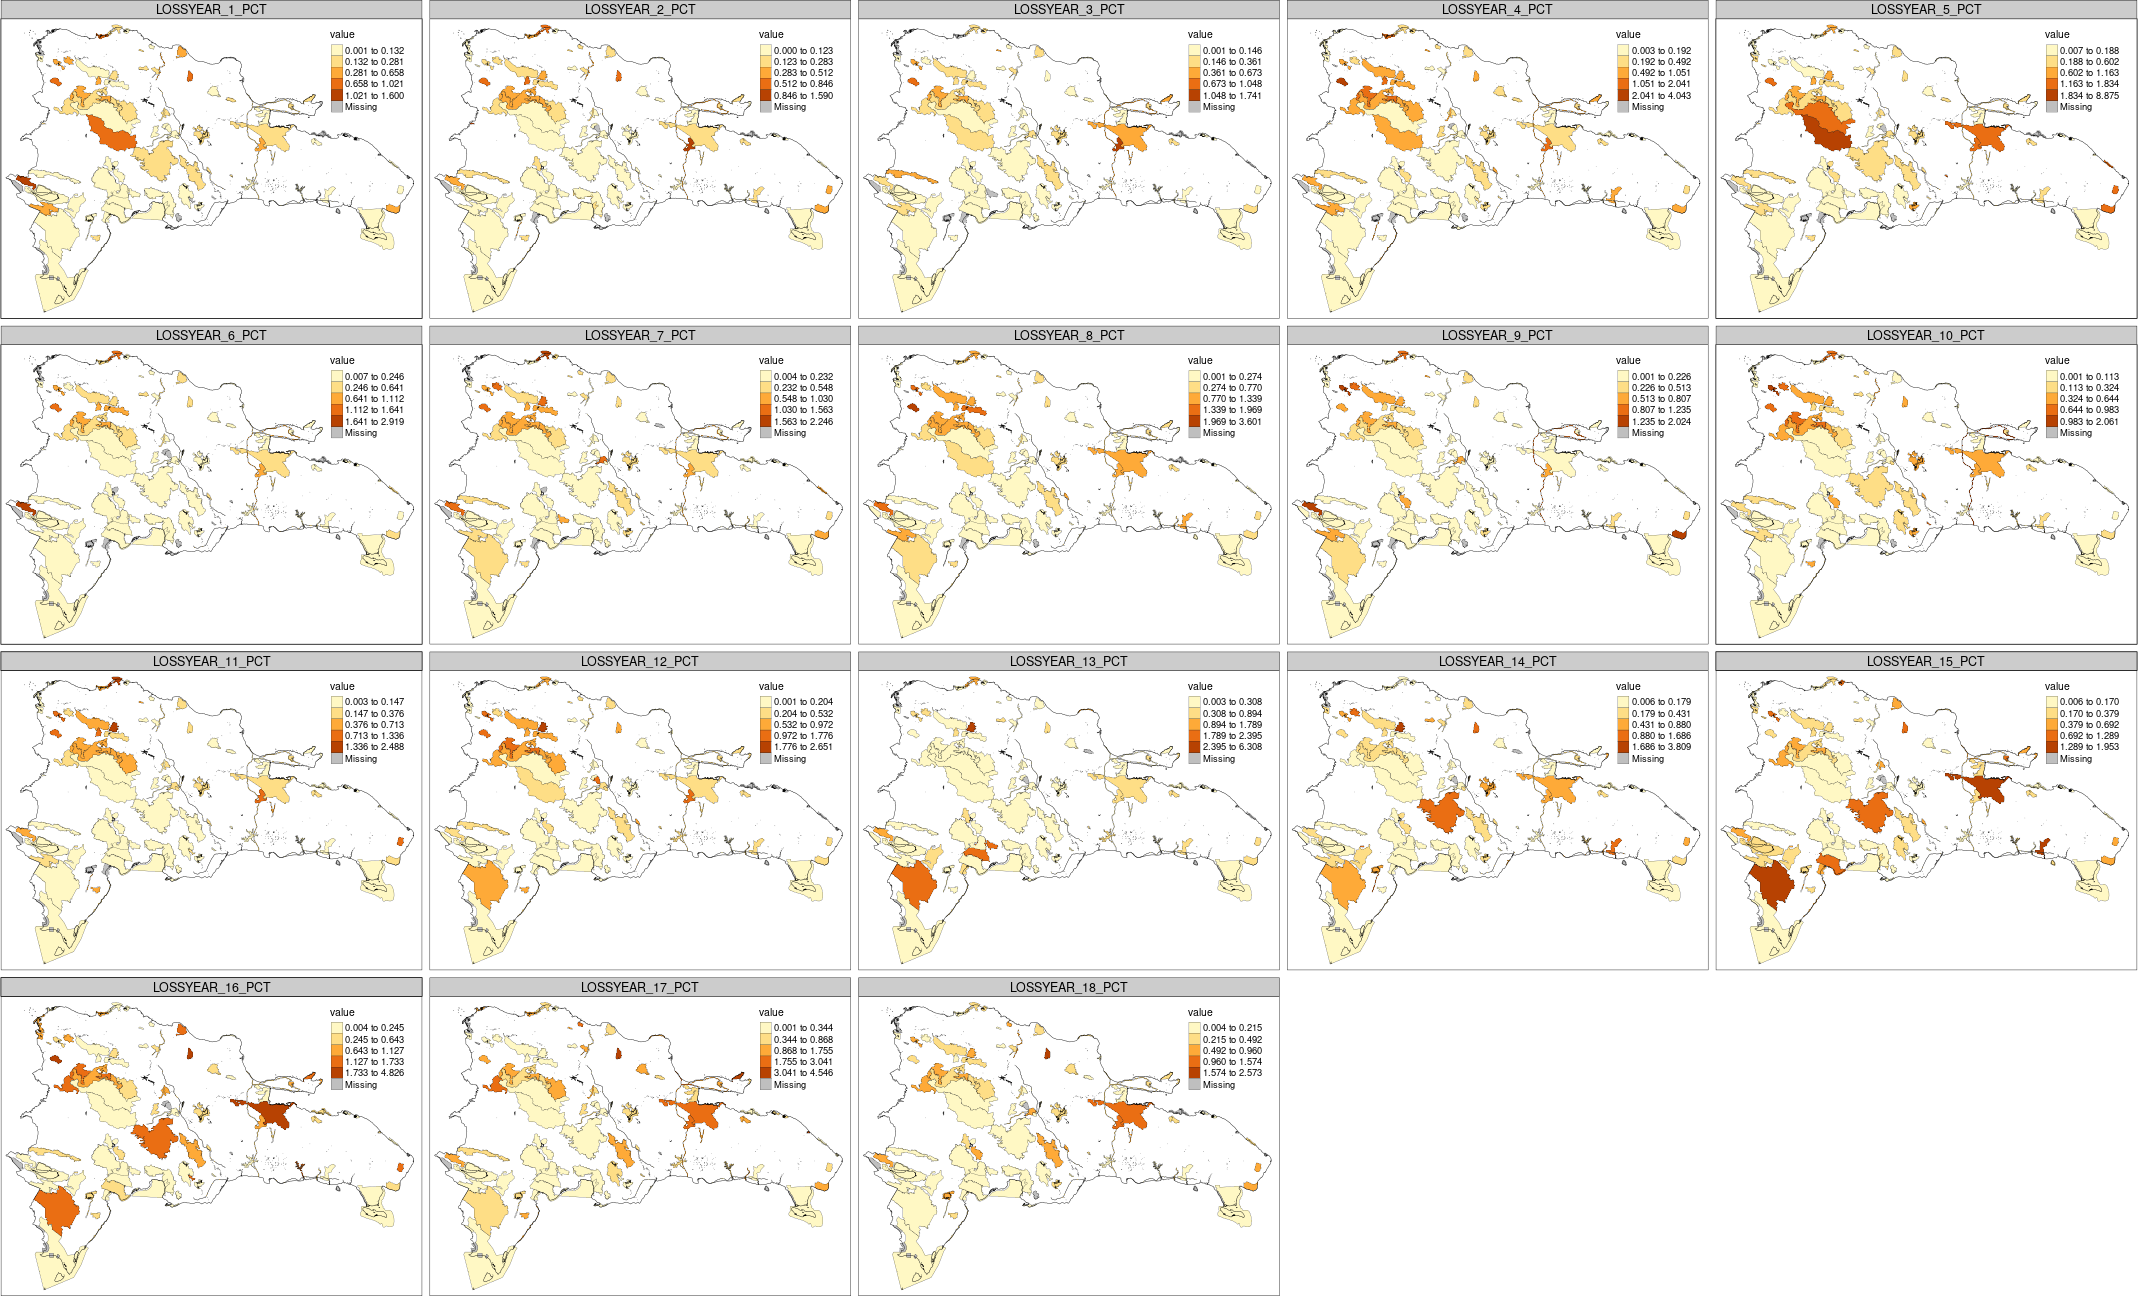
\includegraphics{img/data-download-preparation-eda/zonal-pa-2} \end{center}

\begin{Shaded}
\begin{Highlighting}[]
\CommentTok{\# Top twenty sorted descending by column 2}
\FunctionTok{stripped\_table}\NormalTok{(pazonal }\SpecialCharTok{\%\textgreater{}\%} \FunctionTok{select}\NormalTok{(CATEGORY\_NAME, }\FunctionTok{matches}\NormalTok{(}\StringTok{\textquotesingle{}\^{}LOSSYEAR\_[1{-}9].*\_PCT$\textquotesingle{}}\NormalTok{)))}
\end{Highlighting}
\end{Shaded}

\begin{table}[H]
\centering
\resizebox{\linewidth}{!}{
\begin{tabular}[t]{llrrrrrrrrrrrrrrrrrr}
\toprule
  & CATEGORY\_NAME & LOSSYEAR\_1\_PCT & LOSSYEAR\_2\_PCT & LOSSYEAR\_3\_PCT & LOSSYEAR\_4\_PCT & LOSSYEAR\_5\_PCT & LOSSYEAR\_6\_PCT & LOSSYEAR\_7\_PCT & LOSSYEAR\_8\_PCT & LOSSYEAR\_9\_PCT & LOSSYEAR\_10\_PCT & LOSSYEAR\_11\_PCT & LOSSYEAR\_12\_PCT & LOSSYEAR\_13\_PCT & LOSSYEAR\_14\_PCT & LOSSYEAR\_15\_PCT & LOSSYEAR\_16\_PCT & LOSSYEAR\_17\_PCT & LOSSYEAR\_18\_PCT\\
\midrule
\cellcolor{lightgray}{1} & \cellcolor{lightgray}{Monumento Natural Las Caobas} & \cellcolor{lightgray}{1.6004519} & \cellcolor{lightgray}{0.3431034} & \cellcolor{lightgray}{0.2921958} & \cellcolor{lightgray}{0.8863505} & \cellcolor{lightgray}{0.5690496} & \cellcolor{lightgray}{2.9191685} & \cellcolor{lightgray}{1.4777157} & \cellcolor{lightgray}{1.6157939} & \cellcolor{lightgray}{2.0244496} & \cellcolor{lightgray}{0.2810380} & \cellcolor{lightgray}{0.4358529} & \cellcolor{lightgray}{0.2803406} & \cellcolor{lightgray}{1.7894377} & \cellcolor{lightgray}{0.2705775} & \cellcolor{lightgray}{0.4372476} & \cellcolor{lightgray}{0.1617886} & \cellcolor{lightgray}{1.5453601} & \cellcolor{lightgray}{0.9595738}\\
2 & Reserva Forestal Cerro Chacuey & 1.0207843 & 0.7358154 & 1.0477217 & 4.0434400 & 1.7636884 & 1.5014036 & 1.3015000 & 3.6011002 & 0.8067032 & 0.9825049 & 1.0689880 & 1.0973431 & 0.3048175 & 0.2977288 & 0.3516035 & 4.8260413 & 1.3596280 & 0.3558567\\
\cellcolor{lightgray}{3} & \cellcolor{lightgray}{Reserva Cientifica La Salcedoa} & \cellcolor{lightgray}{0.9838056} & \cellcolor{lightgray}{0.6552752} & \cellcolor{lightgray}{0.0928455} & \cellcolor{lightgray}{0.8641777} & \cellcolor{lightgray}{0.4428018} & \cellcolor{lightgray}{0.4553002} & \cellcolor{lightgray}{0.2749656} & \cellcolor{lightgray}{0.7695467} & \cellcolor{lightgray}{0.4570857} & \cellcolor{lightgray}{0.4713697} & \cellcolor{lightgray}{0.3071045} & \cellcolor{lightgray}{0.8695342} & \cellcolor{lightgray}{0.4874391} & \cellcolor{lightgray}{1.4158944} & \cellcolor{lightgray}{1.2891246} & \cellcolor{lightgray}{4.5922831} & \cellcolor{lightgray}{4.5458603} & \cellcolor{lightgray}{2.5728927}\\
4 & Santuario De Mamiferos Marinos Estero Hondo & 0.8517657 & 0.4021599 & NA & 1.6786787 & 0.1061883 & 0.3298615 & 0.0406679 & 0.6100178 & 0.1852647 & 0.0542238 & 0.4654210 & 0.0180746 & 0.0474458 & 0.0361492 & 0.1355595 & 1.1274034 & 1.6131583 & 0.1174849\\
\cellcolor{lightgray}{5} & \cellcolor{lightgray}{Parque Nacional José del Carmen Ramírez} & \cellcolor{lightgray}{0.7393416} & \cellcolor{lightgray}{0.0711377} & \cellcolor{lightgray}{0.1653339} & \cellcolor{lightgray}{0.5275965} & \cellcolor{lightgray}{8.8746504} & \cellcolor{lightgray}{0.1188245} & \cellcolor{lightgray}{0.1854487} & \cellcolor{lightgray}{0.4381102} & \cellcolor{lightgray}{0.0808517} & \cellcolor{lightgray}{0.0924300} & \cellcolor{lightgray}{0.1257911} & \cellcolor{lightgray}{0.4098513} & \cellcolor{lightgray}{0.0030418} & \cellcolor{lightgray}{0.0140313} & \cellcolor{lightgray}{0.0169749} & \cellcolor{lightgray}{0.0827160} & \cellcolor{lightgray}{0.0977285} & \cellcolor{lightgray}{0.0075553}\\
\addlinespace
6 & Refugio de Vida Silvestre Cañón Río Gurabo & 0.6584242 & 0.8461970 & 0.3560368 & 1.8728510 & 1.1632160 & 1.0900578 & 0.7657229 & 1.1168825 & 0.3731070 & 0.3243349 & 1.2022338 & 0.7218280 & 0.3755456 & 0.3316507 & 0.2511766 & 0.1804570 & 0.1316848 & 0.0560880\\
\cellcolor{lightgray}{7} & \cellcolor{lightgray}{Parque Nacional Punta Espada} & \cellcolor{lightgray}{0.5804178} & \cellcolor{lightgray}{0.4480575} & \cellcolor{lightgray}{0.3398440} & \cellcolor{lightgray}{0.5249696} & \cellcolor{lightgray}{1.4461258} & \cellcolor{lightgray}{0.4730987} & \cellcolor{lightgray}{0.7825356} & \cellcolor{lightgray}{0.4471632} & \cellcolor{lightgray}{1.7537741} & \cellcolor{lightgray}{0.1529298} & \cellcolor{lightgray}{0.3434213} & \cellcolor{lightgray}{0.2808185} & \cellcolor{lightgray}{0.5687916} & \cellcolor{lightgray}{0.2468341} & \cellcolor{lightgray}{0.6743221} & \cellcolor{lightgray}{0.6179795} & \cellcolor{lightgray}{1.0544108} & \cellcolor{lightgray}{0.8353009}\\
8 & Monumento Natural Salto de Socoa & 0.5684204 & 1.1616015 & 1.7407874 & 1.2789458 & 1.3187783 & 0.7955732 & 1.0302619 & 1.2218885 & 0.7212910 & 0.6416260 & 0.8354057 & 1.1239221 & 0.8935396 & 0.6448557 & 0.3197365 & 1.0744006 & 2.5019109 & 1.5739216\\
\cellcolor{lightgray}{9} & \cellcolor{lightgray}{Monumento Natural Lagunas Cabarete y Goleta} & \cellcolor{lightgray}{0.4733122} & \cellcolor{lightgray}{0.2243623} & \cellcolor{lightgray}{0.2059215} & \cellcolor{lightgray}{0.4313083} & \cellcolor{lightgray}{0.4087696} & \cellcolor{lightgray}{0.5409282} & \cellcolor{lightgray}{0.4640918} & \cellcolor{lightgray}{0.4886794} & \cellcolor{lightgray}{0.4200389} & \cellcolor{lightgray}{0.0737629} & \cellcolor{lightgray}{0.2366561} & \cellcolor{lightgray}{0.3319332} & \cellcolor{lightgray}{0.0440529} & \cellcolor{lightgray}{0.2755865} & \cellcolor{lightgray}{0.6915275} & \cellcolor{lightgray}{1.3205614} & \cellcolor{lightgray}{0.5583444} & \cellcolor{lightgray}{0.2971007}\\
10 & Reserva Forestal Las Matas & 0.4634477 & 0.1678266 & 0.0508099 & 0.3033196 & 0.1431915 & 0.2463509 & 1.5627887 & 0.6328139 & 1.0439121 & 0.7590688 & 0.1801441 & 0.4819240 & 0.7482909 & 1.1378333 & 0.0631274 & 0.8406725 & 0.0215557 & 0.1216358\\
\addlinespace
\cellcolor{lightgray}{11} & \cellcolor{lightgray}{Reserva Forestal Alto Mao} & \cellcolor{lightgray}{0.4369518} & \cellcolor{lightgray}{0.4775660} & \cellcolor{lightgray}{0.5342857} & \cellcolor{lightgray}{2.0405091} & \cellcolor{lightgray}{0.9407769} & \cellcolor{lightgray}{0.8367908} & \cellcolor{lightgray}{1.0125519} & \cellcolor{lightgray}{1.1382455} & \cellcolor{lightgray}{0.6956918} & \cellcolor{lightgray}{0.8553472} & \cellcolor{lightgray}{0.5139786} & \cellcolor{lightgray}{1.0657704} & \cellcolor{lightgray}{0.2205767} & \cellcolor{lightgray}{0.2779966} & \cellcolor{lightgray}{0.4929713} & \cellcolor{lightgray}{1.4057385} & \cellcolor{lightgray}{1.0724227} & \cellcolor{lightgray}{0.5647462}\\
12 & Via Panoramica Carretera Santiago - La Cumbre - Puerto Plata & 0.4204920 & 0.3574182 & 0.1051230 & 0.3013526 & 0.1156353 & 0.5396314 & 0.2242624 & 0.3013526 & 0.1927255 & 0.4239961 & 0.3434018 & 0.3784428 & 0.0560656 & 0.1051230 & 0.0770902 & 0.2873362 & 0.7358610 & 0.6307380\\
\cellcolor{lightgray}{13} & \cellcolor{lightgray}{Reserva Biológica Loma Charco Azul} & \cellcolor{lightgray}{0.3784711} & \cellcolor{lightgray}{0.0996866} & \cellcolor{lightgray}{0.2124676} & \cellcolor{lightgray}{0.5968523} & \cellcolor{lightgray}{0.2716037} & \cellcolor{lightgray}{0.1305218} & \cellcolor{lightgray}{0.2433028} & \cellcolor{lightgray}{1.3183128} & \cellcolor{lightgray}{0.6948492} & \cellcolor{lightgray}{0.1279874} & \cellcolor{lightgray}{0.1879683} & \cellcolor{lightgray}{0.1579779} & \cellcolor{lightgray}{0.3083526} & \cellcolor{lightgray}{0.1972612} & \cellcolor{lightgray}{0.3370758} & \cellcolor{lightgray}{0.0604033} & \cellcolor{lightgray}{0.0274560} & \cellcolor{lightgray}{0.0084480}\\
14 & Refugio de Vida Silvestre Río Chacuey & 0.3661892 & 0.2125036 & 0.5141827 & 0.6204345 & 0.1764538 & 0.8443222 & 0.5976663 & 1.9694526 & 1.7000285 & 1.4268096 & 1.3357366 & 1.7759226 & 0.6678683 & 0.4857224 & 0.8917560 & 0.4629542 & 0.0512285 & 0.7627360\\
\cellcolor{lightgray}{15} & \cellcolor{lightgray}{Refugio de Vida Silvestre Monumento Natural Miguel Domingo Fuerte} & \cellcolor{lightgray}{0.2808064} & \cellcolor{lightgray}{0.2654498} & \cellcolor{lightgray}{0.0658140} & \cellcolor{lightgray}{0.1755040} & \cellcolor{lightgray}{0.3663647} & \cellcolor{lightgray}{0.1996358} & \cellcolor{lightgray}{0.2873878} & \cellcolor{lightgray}{0.5023803} & \cellcolor{lightgray}{0.1908606} & \cellcolor{lightgray}{0.4365663} & \cellcolor{lightgray}{0.4694733} & \cellcolor{lightgray}{0.6274269} & \cellcolor{lightgray}{0.0351008} & \cellcolor{lightgray}{0.0548450} & \cellcolor{lightgray}{0.2895816} & \cellcolor{lightgray}{0.6427835} & \cellcolor{lightgray}{1.4237764} & \cellcolor{lightgray}{0.2500932}\\
\addlinespace
16 & Parque Nacional Aniana Vargas & 0.2746660 & 0.0680990 & 0.1810299 & 0.2990682 & 0.3705721 & 0.2304017 & 0.4102966 & 0.3246053 & 0.1038510 & 0.4647758 & 0.2434540 & 0.1588977 & 0.1310906 & 0.5237949 & 0.1265507 & 0.2712611 & 0.7615740 & 0.3989467\\
\cellcolor{lightgray}{17} & \cellcolor{lightgray}{Monumento Natural La Tinaja} & \cellcolor{lightgray}{0.2740955} & \cellcolor{lightgray}{0.2142928} & \cellcolor{lightgray}{0.2392106} & \cellcolor{lightgray}{0.1918668} & \cellcolor{lightgray}{0.2342271} & \cellcolor{lightgray}{0.1719326} & \cellcolor{lightgray}{0.2417024} & \cellcolor{lightgray}{0.2242599} & \cellcolor{lightgray}{0.1669491} & \cellcolor{lightgray}{0.1046546} & \cellcolor{lightgray}{0.0647862} & \cellcolor{lightgray}{0.0697698} & \cellcolor{lightgray}{0.0348849} & \cellcolor{lightgray}{0.4310774} & \cellcolor{lightgray}{0.1146217} & \cellcolor{lightgray}{0.5456992} & \cellcolor{lightgray}{1.2508721} & \cellcolor{lightgray}{0.4136350}\\
18 & Parque Nacional La Hispaniola & 0.2711153 & 0.6451358 & 0.2374733 & 0.4195361 & 1.0547772 & 1.6405446 & 2.2461015 & 0.9954088 & 1.2348611 & 0.9202090 & 2.2797435 & 0.7104409 & 1.6979340 & 0.0771788 & 0.2453891 & 0.2453891 & 0.5066097 & 0.4056835\\
\cellcolor{lightgray}{19} & \cellcolor{lightgray}{Parque Nacional Manolo Tavarez Justo} & \cellcolor{lightgray}{0.2691917} & \cellcolor{lightgray}{0.3497191} & \cellcolor{lightgray}{0.2781856} & \cellcolor{lightgray}{1.0102531} & \cellcolor{lightgray}{0.6017595} & \cellcolor{lightgray}{0.4469795} & \cellcolor{lightgray}{0.7199361} & \cellcolor{lightgray}{0.9751139} & \cellcolor{lightgray}{0.3898782} & \cellcolor{lightgray}{0.4996883} & \cellcolor{lightgray}{0.5084732} & \cellcolor{lightgray}{0.8611205} & \cellcolor{lightgray}{0.1746504} & \cellcolor{lightgray}{0.2610343} & \cellcolor{lightgray}{0.2729566} & \cellcolor{lightgray}{1.1104418} & \cellcolor{lightgray}{0.7075955} & \cellcolor{lightgray}{0.4419596}\\
20 & Monumento Natural Salto de La Damajagua & 0.2659221 & 0.1861455 & 0.4653636 & 0.6913974 & 0.5717325 & 0.2393299 & 0.2925143 & 0.4121792 & 0.7179896 & 0.1462571 & 0.4653636 & 0.3324026 & 0.1196649 & 0.1196649 & 0.0398883 & 0.0664805 & 1.7550858 & 0.0132961\\
\bottomrule
\end{tabular}}
\end{table}

\begin{Shaded}
\begin{Highlighting}[]
\DocumentationTok{\#\# ggplot}
\NormalTok{pazonal }\SpecialCharTok{\%\textgreater{}\%} \FunctionTok{select}\NormalTok{(CATEGORY\_NAME, }\FunctionTok{matches}\NormalTok{(}\StringTok{\textquotesingle{}\^{}LOSSYEAR\_[1{-}9].*\_PCT$|\^{}LOSS0118\_PCT$\textquotesingle{}}\NormalTok{)) }\SpecialCharTok{\%\textgreater{}\%}
  \FunctionTok{st\_drop\_geometry}\NormalTok{() }\SpecialCharTok{\%\textgreater{}\%} 
  \FunctionTok{replace}\NormalTok{(}\FunctionTok{is.na}\NormalTok{(.), }\DecValTok{0}\NormalTok{) }\SpecialCharTok{\%\textgreater{}\%}
  \FunctionTok{arrange}\NormalTok{(}\FunctionTok{desc}\NormalTok{(LOSS0118\_PCT)) }\SpecialCharTok{\%\textgreater{}\%} 
  \FunctionTok{slice}\NormalTok{(}\FunctionTok{c}\NormalTok{(}\DecValTok{1}\SpecialCharTok{:}\DecValTok{10}\NormalTok{,}\DecValTok{37}\NormalTok{)) }\SpecialCharTok{\%\textgreater{}\%} 
  \FunctionTok{mutate}\NormalTok{(}\AttributeTok{CATEGORY\_NAME =} \FunctionTok{gsub}\NormalTok{(}\StringTok{\textquotesingle{}Valle Nuevo\textquotesingle{}}\NormalTok{, }\StringTok{\textquotesingle{}Valle Nuevo (\#37!!)\textquotesingle{}}\NormalTok{, CATEGORY\_NAME)) }\SpecialCharTok{\%\textgreater{}\%} 
  \FunctionTok{mutate}\NormalTok{(}\AttributeTok{CATEGORY\_NAME =} \FunctionTok{fct\_reorder}\NormalTok{(CATEGORY\_NAME, }\FunctionTok{desc}\NormalTok{(LOSS0118\_PCT))) }\SpecialCharTok{\%\textgreater{}\%} 
  \FunctionTok{gather}\NormalTok{(variable, value, }\SpecialCharTok{{-}}\NormalTok{CATEGORY\_NAME, }\SpecialCharTok{{-}}\NormalTok{LOSS0118\_PCT) }\SpecialCharTok{\%\textgreater{}\%}
  \FunctionTok{mutate}\NormalTok{(}\AttributeTok{year =}\NormalTok{ lubridate}\SpecialCharTok{::}\FunctionTok{as\_date}\NormalTok{(}
    \FunctionTok{paste0}\NormalTok{(}\DecValTok{2000} \SpecialCharTok{+} \FunctionTok{as.numeric}\NormalTok{(}\FunctionTok{gsub}\NormalTok{(}\StringTok{\textquotesingle{}(LOSSYEAR\_)([0{-}9]\{,2\})(.*)\textquotesingle{}}\NormalTok{, }\StringTok{\textquotesingle{}}\SpecialCharTok{\textbackslash{}\textbackslash{}}\StringTok{2\textquotesingle{}}\NormalTok{, variable)), }\StringTok{\textquotesingle{}{-}01{-}01\textquotesingle{}}\NormalTok{))) }\SpecialCharTok{\%\textgreater{}\%} 
\NormalTok{  ggplot }\SpecialCharTok{+} \FunctionTok{aes}\NormalTok{(}\AttributeTok{x=}\NormalTok{year, }\AttributeTok{y=}\NormalTok{value, }\AttributeTok{group =}\NormalTok{ CATEGORY\_NAME, }\AttributeTok{colour =}\NormalTok{ CATEGORY\_NAME) }\SpecialCharTok{+} 
  \FunctionTok{geom\_path}\NormalTok{(}\AttributeTok{lwd =} \FloatTok{1.5}\NormalTok{) }\SpecialCharTok{+} 
  \FunctionTok{geom\_point}\NormalTok{(}\AttributeTok{size =} \DecValTok{2}\NormalTok{) }\SpecialCharTok{+} 
  \FunctionTok{scale\_x\_date}\NormalTok{(}\AttributeTok{breaks=}\FunctionTok{date\_breaks}\NormalTok{(}\StringTok{"1 year"}\NormalTok{), }\AttributeTok{date\_labels =} \StringTok{"\%y"}\NormalTok{) }\SpecialCharTok{+} 
  \FunctionTok{scale\_y\_continuous}\NormalTok{(}\AttributeTok{n.breaks =} \DecValTok{3}\NormalTok{, }\AttributeTok{trans =} \StringTok{\textquotesingle{}log1p\textquotesingle{}}\NormalTok{) }\SpecialCharTok{+}
  \FunctionTok{facet\_grid}\NormalTok{(CATEGORY\_NAME }\SpecialCharTok{\textasciitilde{}}\NormalTok{ ., }\AttributeTok{switch =} \StringTok{\textquotesingle{}y\textquotesingle{}}\NormalTok{) }\SpecialCharTok{+}
  \FunctionTok{ggtitle}\NormalTok{(}\StringTok{\textquotesingle{}2001{-}2018 LOSS PCT\textquotesingle{}}\NormalTok{) }\SpecialCharTok{+}
  \FunctionTok{ylab}\NormalTok{(}\StringTok{\textquotesingle{}value (log)\textquotesingle{}}\NormalTok{) }\SpecialCharTok{+}
  \FunctionTok{theme\_bw}\NormalTok{() }\SpecialCharTok{+}
  \FunctionTok{theme}\NormalTok{(}\AttributeTok{strip.text.y.left =} \FunctionTok{element\_text}\NormalTok{(}\AttributeTok{angle =} \DecValTok{0}\NormalTok{), }\AttributeTok{legend.position=}\StringTok{"none"}\NormalTok{,}
        \AttributeTok{axis.text.y =} \FunctionTok{element\_text}\NormalTok{(}\AttributeTok{size =} \DecValTok{8}\NormalTok{), }\AttributeTok{aspect.ratio=}\FloatTok{0.15}\NormalTok{)}
\end{Highlighting}
\end{Shaded}

\begin{center}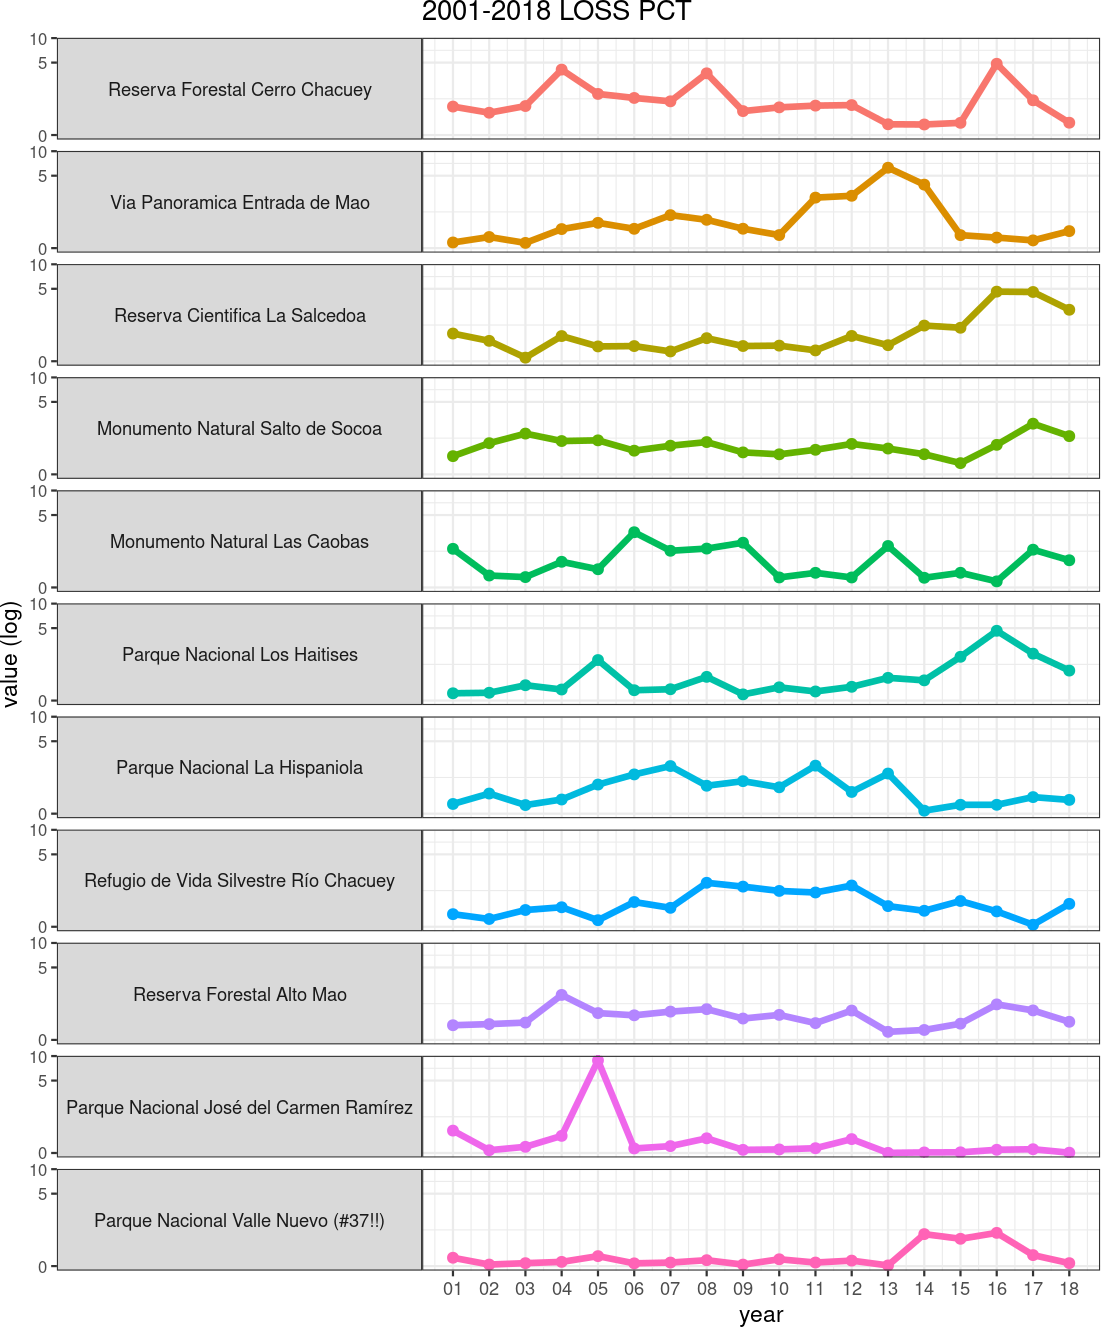
\includegraphics{img/data-download-preparation-eda/zonal-pa-3} \end{center}

\begin{Shaded}
\begin{Highlighting}[]
\CommentTok{\# * AREASQM}
\NormalTok{pazonal }\SpecialCharTok{\%\textgreater{}\%} \FunctionTok{select}\NormalTok{(}\FunctionTok{matches}\NormalTok{(}\StringTok{\textquotesingle{}\^{}LOSSYEAR\_[1{-}9].*\_AREASQM$\textquotesingle{}}\NormalTok{)) }\SpecialCharTok{\%\textgreater{}\%}
  \FunctionTok{gather}\NormalTok{(variable, value, }\SpecialCharTok{{-}}\NormalTok{geom) }\SpecialCharTok{\%\textgreater{}\%}
  \FunctionTok{mutate}\NormalTok{(}\AttributeTok{variable =} \FunctionTok{factor}\NormalTok{(variable, }\AttributeTok{levels =} \FunctionTok{unique}\NormalTok{(variable))) }\SpecialCharTok{\%\textgreater{}\%} 
  \FunctionTok{tm\_shape}\NormalTok{() }\SpecialCharTok{+}
  \FunctionTok{tm\_fill}\NormalTok{(}\AttributeTok{col=}\StringTok{\textquotesingle{}value\textquotesingle{}}\NormalTok{, }\AttributeTok{palette =} \StringTok{"YlOrBr"}\NormalTok{, }\AttributeTok{size =} \FloatTok{0.1}\NormalTok{, }\AttributeTok{style =} \StringTok{\textquotesingle{}jenks\textquotesingle{}}\NormalTok{) }\SpecialCharTok{+}
  \FunctionTok{tm\_borders}\NormalTok{(}\AttributeTok{col =} \StringTok{\textquotesingle{}grey15\textquotesingle{}}\NormalTok{, }\AttributeTok{lwd =} \FloatTok{0.3}\NormalTok{) }\SpecialCharTok{+}
  \FunctionTok{tm\_facets}\NormalTok{(}\AttributeTok{by =} \StringTok{"variable"}\NormalTok{, }\AttributeTok{ncol =} \DecValTok{5}\NormalTok{, }\AttributeTok{nrow =} \DecValTok{4}\NormalTok{, }\AttributeTok{free.coords =} \ConstantTok{FALSE}\NormalTok{, }\AttributeTok{free.scales =} \ConstantTok{TRUE}\NormalTok{) }\SpecialCharTok{+}
  \FunctionTok{tm\_layout}\NormalTok{(}\AttributeTok{panel.label.size =} \DecValTok{1}\NormalTok{, }\AttributeTok{legend.title.size =} \DecValTok{1}\NormalTok{, }\AttributeTok{legend.text.size =} \FloatTok{0.75}\NormalTok{) }\SpecialCharTok{+} 
  \FunctionTok{tm\_shape}\NormalTok{(}\AttributeTok{shp =}\NormalTok{ cline) }\SpecialCharTok{+} \FunctionTok{tm\_borders}\NormalTok{(}\AttributeTok{col =} \StringTok{\textquotesingle{}black\textquotesingle{}}\NormalTok{, }\AttributeTok{lwd =} \FloatTok{0.5}\NormalTok{)}
\end{Highlighting}
\end{Shaded}

\begin{center}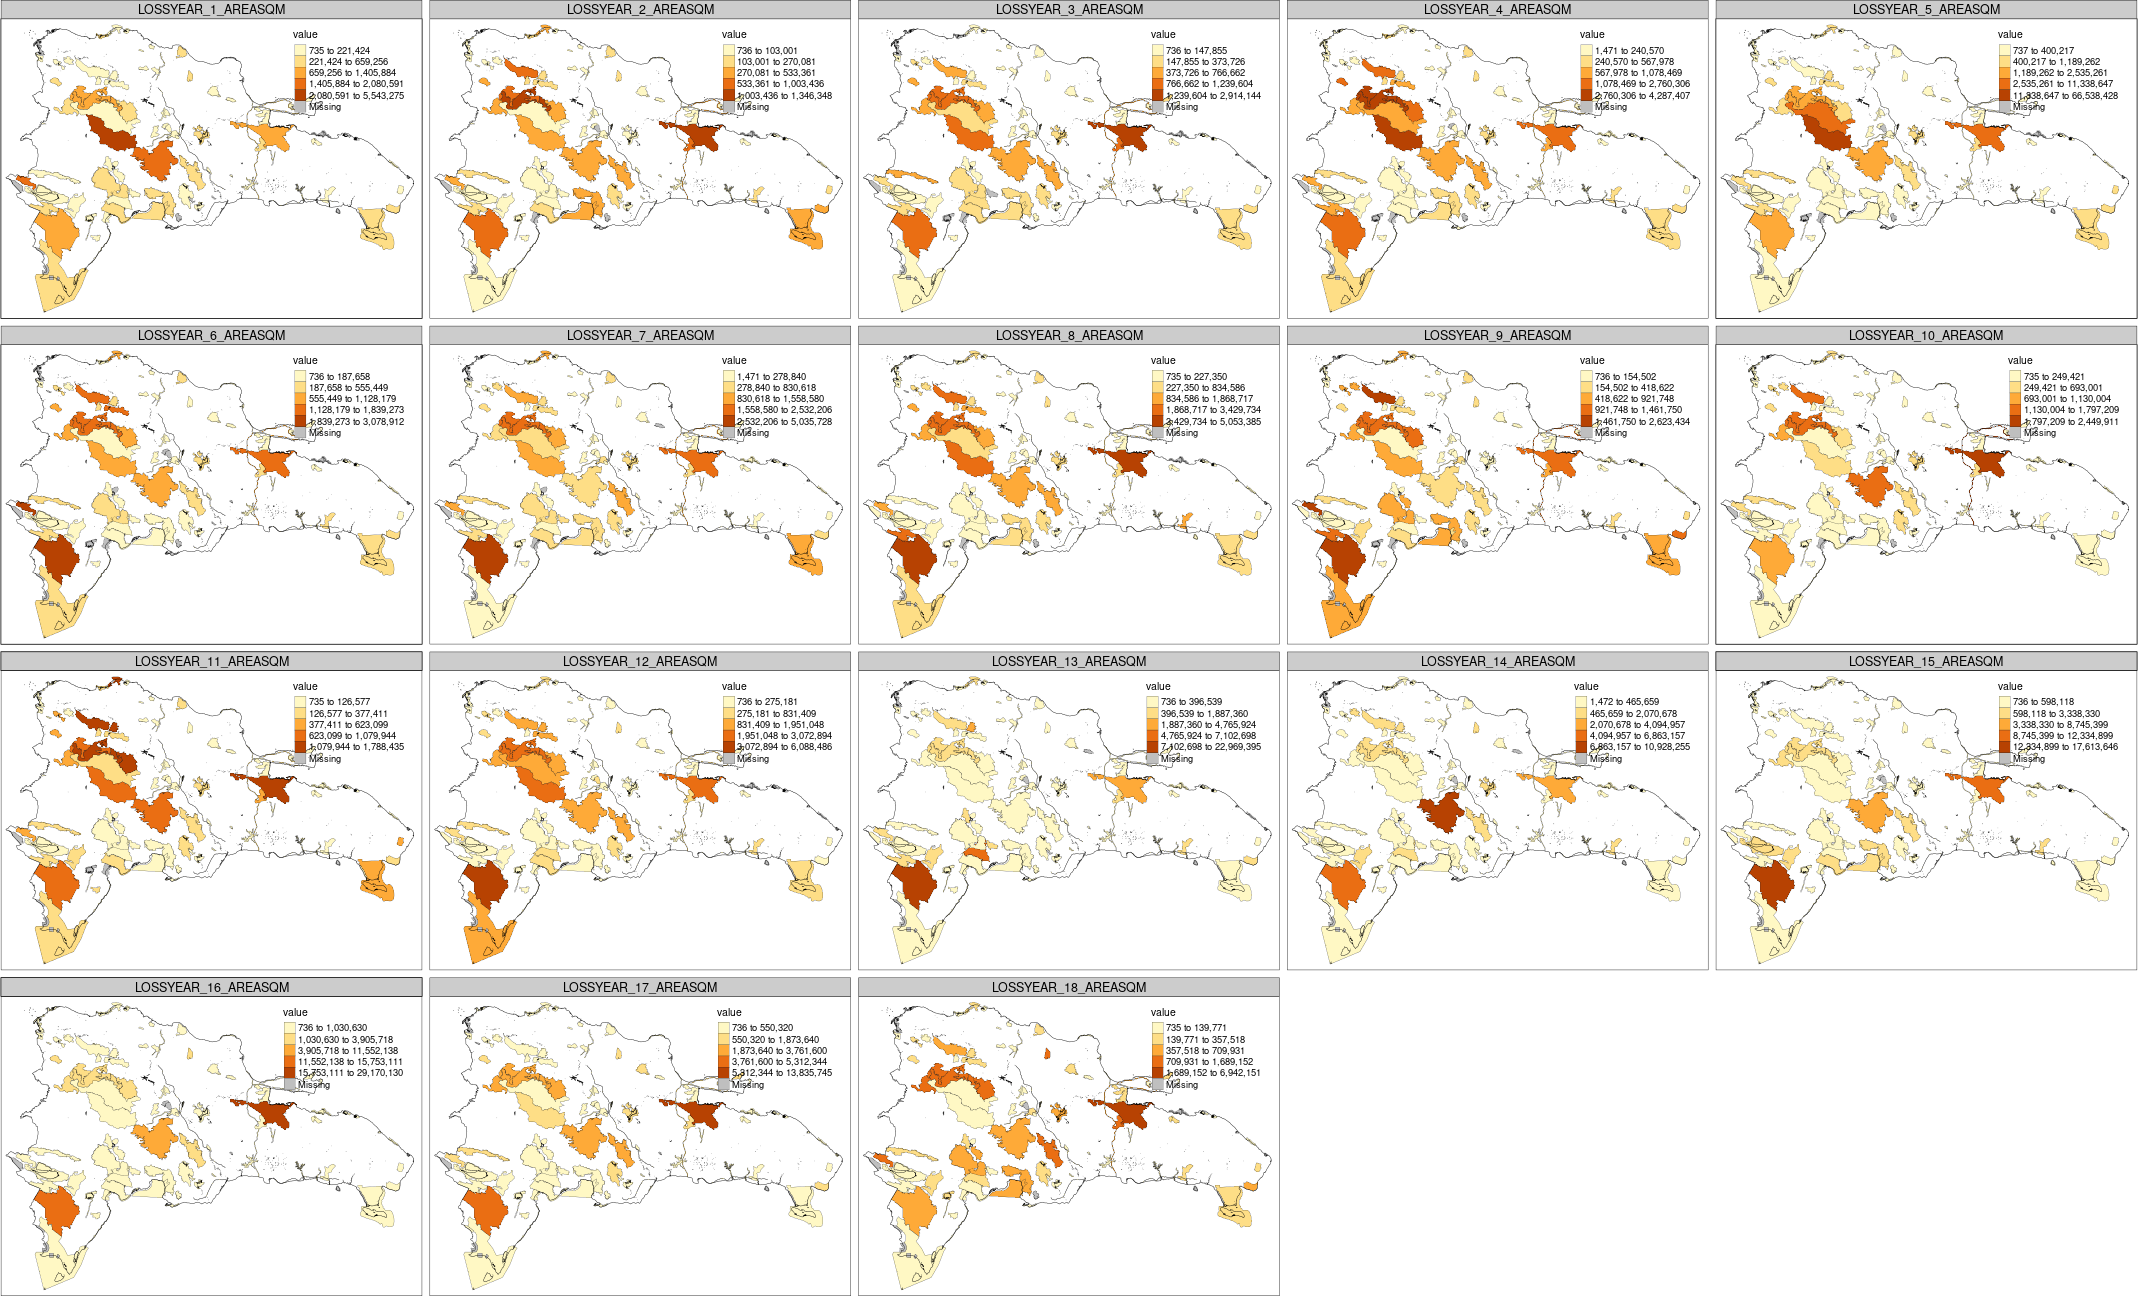
\includegraphics{img/data-download-preparation-eda/zonal-pa-4} \end{center}

\begin{Shaded}
\begin{Highlighting}[]
\CommentTok{\# Top twenty sorted descending by column 2}
\FunctionTok{stripped\_table}\NormalTok{(pazonal }\SpecialCharTok{\%\textgreater{}\%} \FunctionTok{select}\NormalTok{(CATEGORY\_NAME, }\FunctionTok{matches}\NormalTok{(}\StringTok{\textquotesingle{}\^{}LOSSYEAR\_[1{-}9].*\_AREASQM$\textquotesingle{}}\NormalTok{)))}
\end{Highlighting}
\end{Shaded}

\begin{table}[H]
\centering
\resizebox{\linewidth}{!}{
\begin{tabular}[t]{llrrrrrrrrrrrrrrrrrr}
\toprule
  & CATEGORY\_NAME & LOSSYEAR\_1\_AREASQM & LOSSYEAR\_2\_AREASQM & LOSSYEAR\_3\_AREASQM & LOSSYEAR\_4\_AREASQM & LOSSYEAR\_5\_AREASQM & LOSSYEAR\_6\_AREASQM & LOSSYEAR\_7\_AREASQM & LOSSYEAR\_8\_AREASQM & LOSSYEAR\_9\_AREASQM & LOSSYEAR\_10\_AREASQM & LOSSYEAR\_11\_AREASQM & LOSSYEAR\_12\_AREASQM & LOSSYEAR\_13\_AREASQM & LOSSYEAR\_14\_AREASQM & LOSSYEAR\_15\_AREASQM & LOSSYEAR\_16\_AREASQM & LOSSYEAR\_17\_AREASQM & LOSSYEAR\_18\_AREASQM\\
\midrule
\cellcolor{lightgray}{1} & \cellcolor{lightgray}{Parque Nacional José del Carmen Ramírez} & \cellcolor{lightgray}{5543275.0} & \cellcolor{lightgray}{533360.902} & \cellcolor{lightgray}{1239604.3} & \cellcolor{lightgray}{3955698.72} & \cellcolor{lightgray}{66538427.81} & \cellcolor{lightgray}{890896.6} & \cellcolor{lightgray}{1390416.7} & \cellcolor{lightgray}{3284767.49} & \cellcolor{lightgray}{606192.3} & \cellcolor{lightgray}{693001.34} & \cellcolor{lightgray}{943129.21} & \cellcolor{lightgray}{3072894.47} & \cellcolor{lightgray}{22805.78} & \cellcolor{lightgray}{105200.8} & \cellcolor{lightgray}{127270.9} & \cellcolor{lightgray}{620170.0} & \cellcolor{lightgray}{732727.53} & \cellcolor{lightgray}{56646.61}\\
2 & Parque Nacional Valle Nuevo & 2080591.4 & 353877.104 & 682004.3 & 996153.01 & 2535260.92 & 637861.6 & 830618.0 & 1428751.22 & 342105.7 & 1667857.37 & 835032.25 & 1316187.40 & 154499.36 & 10928254.7 & 8745399.4 & 11552137.8 & 2833223.97 & 686418.58\\
\cellcolor{lightgray}{3} & \cellcolor{lightgray}{Monumento Natural Las Caobas} & \cellcolor{lightgray}{1688032.2} & \cellcolor{lightgray}{361878.800} & \cellcolor{lightgray}{308185.4} & \cellcolor{lightgray}{934853.57} & \cellcolor{lightgray}{600189.23} & \cellcolor{lightgray}{3078911.9} & \cellcolor{lightgray}{1558579.6} & \cellcolor{lightgray}{1704213.78} & \cellcolor{lightgray}{2135232.0} & \cellcolor{lightgray}{296416.98} & \cellcolor{lightgray}{459703.76} & \cellcolor{lightgray}{295681.46} & \cellcolor{lightgray}{1887359.76} & \cellcolor{lightgray}{285384.1} & \cellcolor{lightgray}{461174.8} & \cellcolor{lightgray}{170642.0} & \cellcolor{lightgray}{1629925.65} & \cellcolor{lightgray}{1012083.80}\\
4 & Parque Nacional Sierra de Bahoruco & 1405884.1 & 770992.424 & 1182237.4 & 1873040.76 & 1824485.89 & 2444664.0 & 5035728.2 & 5053384.51 & 2623434.1 & 1130004.16 & 836467.93 & 6088485.98 & 22969394.53 & 6863156.8 & 17613645.6 & 15753111.4 & 5312343.79 & 709931.00\\
\cellcolor{lightgray}{5} & \cellcolor{lightgray}{Parque Nacional Los Haitises} & \cellcolor{lightgray}{1247762.6} & \cellcolor{lightgray}{1346347.660} & \cellcolor{lightgray}{2914143.8} & \cellcolor{lightgray}{1986414.58} & \cellcolor{lightgray}{10892908.99} & \cellcolor{lightgray}{1839272.8} & \cellcolor{lightgray}{2040857.1} & \cellcolor{lightgray}{5036664.52} & \cellcolor{lightgray}{1044706.9} & \cellcolor{lightgray}{2449911.32} & \cellcolor{lightgray}{1593545.92} & \cellcolor{lightgray}{2561739.10} & \cellcolor{lightgray}{4765923.57} & \cellcolor{lightgray}{4094956.9} & \cellcolor{lightgray}{12334898.8} & \cellcolor{lightgray}{29170130.3} & \cellcolor{lightgray}{13835745.41} & \cellcolor{lightgray}{6942151.10}\\
\addlinespace
6 & Parque Nacional Manolo Tavarez Justo & 946818.5 & 1230054.749 & 978452.6 & 3553328.01 & 2116547.55 & 1572145.3 & 2532206.0 & 3429733.99 & 1371305.1 & 1757536.36 & 1788434.86 & 3028789.11 & 614291.70 & 918127.0 & 960060.7 & 3905718.1 & 2488800.97 & 1554489.05\\
\cellcolor{lightgray}{7} & \cellcolor{lightgray}{Reserva Forestal Alto Mao} & \cellcolor{lightgray}{918099.6} & \cellcolor{lightgray}{1003435.754} & \cellcolor{lightgray}{1122612.1} & \cellcolor{lightgray}{4287407.31} & \cellcolor{lightgray}{1976709.58} & \cellcolor{lightgray}{1758219.5} & \cellcolor{lightgray}{2127519.2} & \cellcolor{lightgray}{2391619.97} & \cellcolor{lightgray}{1461749.9} & \cellcolor{lightgray}{1797209.35} & \cellcolor{lightgray}{1079944.05} & \cellcolor{lightgray}{2239339.03} & \cellcolor{lightgray}{463463.73} & \cellcolor{lightgray}{584111.4} & \cellcolor{lightgray}{1035804.6} & \cellcolor{lightgray}{2953661.7} & \cellcolor{lightgray}{2253316.51} & \cellcolor{lightgray}{1186614.28}\\
8 & Reserva Biológica Loma Charco Azul & 659256.4 & 173643.414 & 370095.9 & 1039653.15 & 473104.72 & 227355.1 & 423807.7 & 2296360.57 & 1210353.5 & 222940.48 & 327420.84 & 275180.66 & 537117.34 & 343607.9 & 587150.2 & 105216.1 & 47825.52 & 14715.54\\
\cellcolor{lightgray}{9} & \cellcolor{lightgray}{Parque Nacional Cotubanamá (Del Este)} & \cellcolor{lightgray}{540690.4} & \cellcolor{lightgray}{438437.356} & \cellcolor{lightgray}{237609.5} & \cellcolor{lightgray}{432552.29} & \cellcolor{lightgray}{1037242.74} & \cellcolor{lightgray}{438437.4} & \cellcolor{lightgray}{995311.6} & \cellcolor{lightgray}{712828.52} & \cellcolor{lightgray}{921748.3} & \cellcolor{lightgray}{224368.11} & \cellcolor{lightgray}{559816.82} & \cellcolor{lightgray}{521563.90} & \cellcolor{lightgray}{235402.61} & \cellcolor{lightgray}{183908.3} & \cellcolor{lightgray}{213333.6} & \cellcolor{lightgray}{177287.6} & \cellcolor{lightgray}{387678.67} & \cellcolor{lightgray}{357517.71}\\
10 & Reserva Forestal Cerro Chacuey & 529715.1 & 381836.335 & 543693.7 & 2098260.55 & 915230.06 & 779122.7 & 675386.8 & 1868717.32 & 418622.1 & 509850.83 & 554729.47 & 569443.78 & 158178.83 & 154500.3 & 182457.4 & 2504375.5 & 705551.15 & 184664.59\\
\addlinespace
\cellcolor{lightgray}{11} & \cellcolor{lightgray}{Parque Nacional Punta Espada} & \cellcolor{lightgray}{477322.9} & \cellcolor{lightgray}{368472.701} & \cellcolor{lightgray}{279480.3} & \cellcolor{lightgray}{431723.50} & \cellcolor{lightgray}{1189262.19} & \cellcolor{lightgray}{389066.0} & \cellcolor{lightgray}{643540.1} & \cellcolor{lightgray}{367737.23} & \cellcolor{lightgray}{1442265.4} & \cellcolor{lightgray}{125766.13} & \cellcolor{lightgray}{282422.19} & \cellcolor{lightgray}{230938.98} & \cellcolor{lightgray}{467761.75} & \cellcolor{lightgray}{202990.9} & \cellcolor{lightgray}{554547.7} & \cellcolor{lightgray}{508212.8} & \cellcolor{lightgray}{867124.38} & \cellcolor{lightgray}{686933.14}\\
12 & Reserva Forestal Alto bao & 456127.4 & 464219.973 & 719504.2 & 2760306.40 & 1054978.51 & 773209.5 & 1219772.9 & 1730341.32 & 1215358.8 & 676834.19 & 1488299.53 & 1951048.13 & 156701.83 & 447299.1 & 190543.5 & 1662657.9 & 3226733.44 & 1207266.20\\
\cellcolor{lightgray}{13} & \cellcolor{lightgray}{Parque Nacional Montaña La Humeadora} & \cellcolor{lightgray}{432587.7} & \cellcolor{lightgray}{345775.901} & \cellcolor{lightgray}{587819.0} & \cellcolor{lightgray}{1072640.99} & \cellcolor{lightgray}{837954.79} & \cellcolor{lightgray}{555448.5} & \cellcolor{lightgray}{1104275.8} & \cellcolor{lightgray}{1192559.01} & \cellcolor{lightgray}{357547.0} & \cellcolor{lightgray}{607682.75} & \cellcolor{lightgray}{377410.72} & \cellcolor{lightgray}{1224193.83} & \cellcolor{lightgray}{396538.75} & \cellcolor{lightgray}{715829.7} & \cellcolor{lightgray}{812941.2} & \cellcolor{lightgray}{2205608.8} & \cellcolor{lightgray}{3761600.39} & \cellcolor{lightgray}{1689152.06}\\
14 & Parque Nacional Nalga de Maco & 422265.6 & 361941.939 & 598822.6 & 1078469.27 & 782000.57 & 642961.9 & 733447.4 & 1092446.70 & 663560.2 & 1030651.74 & 623099.23 & 1371259.70 & 136831.71 & 150073.5 & 923246.2 & 2805785.7 & 3523784.32 & 1018145.62\\
\cellcolor{lightgray}{15} & \cellcolor{lightgray}{Parque Nacional Francisco Alberto Caamaño Deñó} & \cellcolor{lightgray}{409038.8} & \cellcolor{lightgray}{481871.299} & \cellcolor{lightgray}{186127.4} & \cellcolor{lightgray}{309721.86} & \cellcolor{lightgray}{331792.30} & \cellcolor{lightgray}{108880.8} & \cellcolor{lightgray}{434052.0} & \cellcolor{lightgray}{359748.19} & \cellcolor{lightgray}{658434.8} & \cellcolor{lightgray}{173620.80} & \cellcolor{lightgray}{126537.20} & \cellcolor{lightgray}{169942.40} & \cellcolor{lightgray}{204519.42} & \cellcolor{lightgray}{240567.8} & \cellcolor{lightgray}{764372.9} & \cellcolor{lightgray}{251603.0} & \cellcolor{lightgray}{356069.78} & \cellcolor{lightgray}{468629.03}\\
\addlinespace
16 & Reserva Cientifica La Salcedoa & 405489.4 & 270080.935 & 38267.6 & 356183.03 & 182507.01 & 187658.4 & 113331.0 & 317179.52 & 188394.3 & 194281.65 & 126577.44 & 358390.78 & 200904.89 & 583580.9 & 531330.9 & 1892774.3 & 1873640.49 & 1060454.02\\
\cellcolor{lightgray}{17} & \cellcolor{lightgray}{Reserva Forestal Cabeza de Toro} & \cellcolor{lightgray}{389901.5} & \cellcolor{lightgray}{2206.989} & \cellcolor{lightgray}{123591.4} & \cellcolor{lightgray}{61795.70} & \cellcolor{lightgray}{83129.93} & \cellcolor{lightgray}{112556.5} & \cellcolor{lightgray}{443604.9} & \cellcolor{lightgray}{30897.85} & \cellcolor{lightgray}{564989.3} & \cellcolor{lightgray}{60324.38} & \cellcolor{lightgray}{66209.68} & \cellcolor{lightgray}{81658.61} & \cellcolor{lightgray}{98578.86} & \cellcolor{lightgray}{183180.1} & \cellcolor{lightgray}{226584.2} & \cellcolor{lightgray}{108878.1} & \cellcolor{lightgray}{11034.95} & \cellcolor{lightgray}{194215.07}\\
18 & Monumento Natural Salto de Socoa & 388248.0 & 793408.359 & 1189009.6 & 873558.04 & 900764.82 & 543400.2 & 703699.5 & 834586.18 & 492663.2 & 438249.66 & 570606.94 & 767672.22 & 610314.12 & 440455.6 & 218389.5 & 733847.6 & 1708879.54 & 1075035.24\\
\cellcolor{lightgray}{19} & \cellcolor{lightgray}{Parque Nacional Anacaona} & \cellcolor{lightgray}{373725.6} & \cellcolor{lightgray}{2207.041} & \cellcolor{lightgray}{373725.6} & \cellcolor{lightgray}{62532.83} & \cellcolor{lightgray}{193483.92} & \cellcolor{lightgray}{251602.7} & \cellcolor{lightgray}{646663.0} & \cellcolor{lightgray}{47083.54} & \cellcolor{lightgray}{656226.8} & \cellcolor{lightgray}{112559.09} & \cellcolor{lightgray}{104466.61} & \cellcolor{lightgray}{153757.19} & \cellcolor{lightgray}{264844.92} & \cellcolor{lightgray}{320020.9} & \cellcolor{lightgray}{275880.1} & \cellcolor{lightgray}{237624.7} & \cellcolor{lightgray}{80189.15} & \cellcolor{lightgray}{512033.50}\\
20 & Reserva Forestal Hatillo & 365633.5 & 520126.470 & 279558.8 & 305307.62 & 300157.85 & 113294.9 & 430373.4 & 359748.01 & 388439.6 & 202312.28 & 112559.19 & 225118.39 & 267787.89 & 404624.6 & 868839.3 & 282501.5 & 347241.43 & 497320.36\\
\bottomrule
\end{tabular}}
\end{table}

\begin{Shaded}
\begin{Highlighting}[]
\DocumentationTok{\#\# ggplot}
\NormalTok{pazonal }\SpecialCharTok{\%\textgreater{}\%} \FunctionTok{select}\NormalTok{(CATEGORY\_NAME, }\FunctionTok{matches}\NormalTok{(}\StringTok{\textquotesingle{}\^{}LOSSYEAR\_[1{-}9].*\_AREASQM$|\^{}LOSS0118\_AREASQM$\textquotesingle{}}\NormalTok{)) }\SpecialCharTok{\%\textgreater{}\%}
  \FunctionTok{st\_drop\_geometry}\NormalTok{() }\SpecialCharTok{\%\textgreater{}\%} 
  \FunctionTok{replace}\NormalTok{(}\FunctionTok{is.na}\NormalTok{(.), }\DecValTok{0}\NormalTok{) }\SpecialCharTok{\%\textgreater{}\%}
  \FunctionTok{arrange}\NormalTok{(}\FunctionTok{desc}\NormalTok{(LOSS0118\_AREASQM)) }\SpecialCharTok{\%\textgreater{}\%} 
  \FunctionTok{slice}\NormalTok{(}\FunctionTok{c}\NormalTok{(}\DecValTok{1}\SpecialCharTok{:}\DecValTok{10}\NormalTok{)) }\SpecialCharTok{\%\textgreater{}\%} 
  \FunctionTok{mutate}\NormalTok{(}\AttributeTok{CATEGORY\_NAME =} \FunctionTok{fct\_reorder}\NormalTok{(CATEGORY\_NAME, }\FunctionTok{desc}\NormalTok{(LOSS0118\_AREASQM))) }\SpecialCharTok{\%\textgreater{}\%} 
  \FunctionTok{gather}\NormalTok{(variable, value, }\SpecialCharTok{{-}}\NormalTok{CATEGORY\_NAME, }\SpecialCharTok{{-}}\NormalTok{LOSS0118\_AREASQM) }\SpecialCharTok{\%\textgreater{}\%}
  \FunctionTok{mutate}\NormalTok{(}\AttributeTok{year =}\NormalTok{ lubridate}\SpecialCharTok{::}\FunctionTok{as\_date}\NormalTok{(}
    \FunctionTok{paste0}\NormalTok{(}\DecValTok{2000} \SpecialCharTok{+} \FunctionTok{as.numeric}\NormalTok{(}\FunctionTok{gsub}\NormalTok{(}\StringTok{\textquotesingle{}(LOSSYEAR\_)([0{-}9]\{,2\})(.*)\textquotesingle{}}\NormalTok{, }\StringTok{\textquotesingle{}}\SpecialCharTok{\textbackslash{}\textbackslash{}}\StringTok{2\textquotesingle{}}\NormalTok{, variable)), }\StringTok{\textquotesingle{}{-}01{-}01\textquotesingle{}}\NormalTok{))) }\SpecialCharTok{\%\textgreater{}\%} 
\NormalTok{  ggplot }\SpecialCharTok{+} \FunctionTok{aes}\NormalTok{(}\AttributeTok{x=}\NormalTok{year, }\AttributeTok{y=}\NormalTok{value, }\AttributeTok{group =}\NormalTok{ CATEGORY\_NAME, }\AttributeTok{colour =}\NormalTok{ CATEGORY\_NAME) }\SpecialCharTok{+} 
  \FunctionTok{geom\_path}\NormalTok{(}\AttributeTok{lwd =} \FloatTok{1.5}\NormalTok{) }\SpecialCharTok{+} 
  \FunctionTok{geom\_point}\NormalTok{(}\AttributeTok{size =} \DecValTok{2}\NormalTok{) }\SpecialCharTok{+} 
  \FunctionTok{scale\_x\_date}\NormalTok{(}\AttributeTok{breaks=}\FunctionTok{date\_breaks}\NormalTok{(}\StringTok{"1 year"}\NormalTok{), }\AttributeTok{date\_labels =} \StringTok{"\%y"}\NormalTok{) }\SpecialCharTok{+} 
  \FunctionTok{scale\_y\_continuous}\NormalTok{(}\AttributeTok{n.breaks =} \DecValTok{3}\NormalTok{, }\AttributeTok{trans =} \StringTok{\textquotesingle{}log2\textquotesingle{}}\NormalTok{) }\SpecialCharTok{+}
  \FunctionTok{facet\_grid}\NormalTok{(CATEGORY\_NAME }\SpecialCharTok{\textasciitilde{}}\NormalTok{ ., }\AttributeTok{switch =} \StringTok{\textquotesingle{}y\textquotesingle{}}\NormalTok{) }\SpecialCharTok{+}
  \FunctionTok{ggtitle}\NormalTok{(}\StringTok{\textquotesingle{}2001{-}2018 LOSS AREA SQM\textquotesingle{}}\NormalTok{) }\SpecialCharTok{+}
  \FunctionTok{ylab}\NormalTok{(}\StringTok{\textquotesingle{}value (log)\textquotesingle{}}\NormalTok{) }\SpecialCharTok{+}
  \FunctionTok{theme\_bw}\NormalTok{() }\SpecialCharTok{+}
  \FunctionTok{theme}\NormalTok{(}\AttributeTok{strip.text.y.left =} \FunctionTok{element\_text}\NormalTok{(}\AttributeTok{angle =} \DecValTok{0}\NormalTok{), }\AttributeTok{legend.position=}\StringTok{"none"}\NormalTok{,}
        \AttributeTok{axis.text.y =} \FunctionTok{element\_text}\NormalTok{(}\AttributeTok{size =} \DecValTok{8}\NormalTok{), }\AttributeTok{aspect.ratio=}\FloatTok{0.15}\NormalTok{)}
\end{Highlighting}
\end{Shaded}

\begin{center}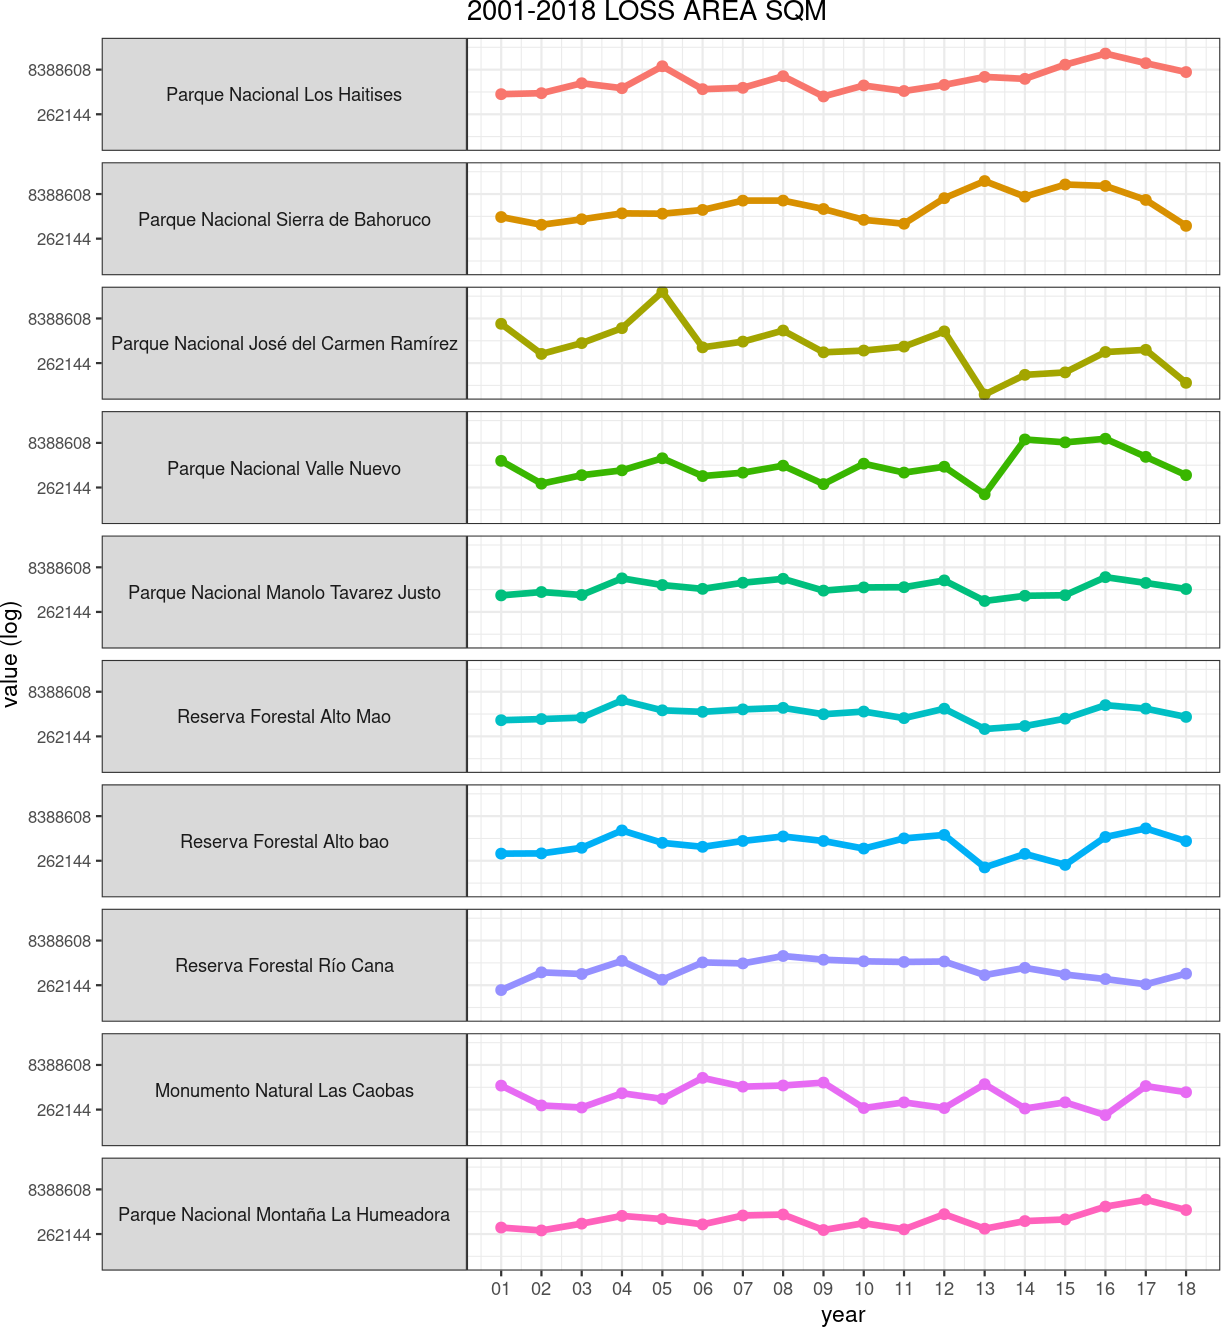
\includegraphics{img/data-download-preparation-eda/zonal-pa-5} \end{center}

\begin{Shaded}
\begin{Highlighting}[]

\CommentTok{\# Total loss 2001{-}2018}
\NormalTok{pazonal }\SpecialCharTok{\%\textgreater{}\%} \FunctionTok{select}\NormalTok{(}\FunctionTok{matches}\NormalTok{(}\StringTok{\textquotesingle{}\^{}LOSS0118\textquotesingle{}}\NormalTok{)) }\SpecialCharTok{\%\textgreater{}\%} \FunctionTok{select}\NormalTok{(}\SpecialCharTok{{-}}\FunctionTok{matches}\NormalTok{(}\StringTok{\textquotesingle{}\textless{}NA\textgreater{}\textquotesingle{}}\NormalTok{)) }\SpecialCharTok{\%\textgreater{}\%} 
  \FunctionTok{gather}\NormalTok{(variable, value, }\SpecialCharTok{{-}}\NormalTok{geom) }\SpecialCharTok{\%\textgreater{}\%}
  \FunctionTok{mutate}\NormalTok{(}\AttributeTok{variable =} \FunctionTok{factor}\NormalTok{(variable, }\AttributeTok{levels =} \FunctionTok{unique}\NormalTok{(variable))) }\SpecialCharTok{\%\textgreater{}\%} 
  \FunctionTok{tm\_shape}\NormalTok{() }\SpecialCharTok{+}
  \FunctionTok{tm\_fill}\NormalTok{(}\AttributeTok{col=}\StringTok{\textquotesingle{}value\textquotesingle{}}\NormalTok{, }\AttributeTok{palette =} \StringTok{"YlOrBr"}\NormalTok{, }\AttributeTok{size =} \FloatTok{0.1}\NormalTok{, }\AttributeTok{style =} \StringTok{\textquotesingle{}jenks\textquotesingle{}}\NormalTok{) }\SpecialCharTok{+}
  \FunctionTok{tm\_borders}\NormalTok{(}\AttributeTok{col =} \StringTok{\textquotesingle{}grey15\textquotesingle{}}\NormalTok{, }\AttributeTok{lwd =} \FloatTok{0.3}\NormalTok{) }\SpecialCharTok{+}
  \FunctionTok{tm\_facets}\NormalTok{(}\AttributeTok{by =} \StringTok{"variable"}\NormalTok{, }\AttributeTok{ncol =} \DecValTok{2}\NormalTok{, }\AttributeTok{nrow =} \DecValTok{1}\NormalTok{, }\AttributeTok{free.coords =} \ConstantTok{FALSE}\NormalTok{, }\AttributeTok{free.scales =} \ConstantTok{TRUE}\NormalTok{) }\SpecialCharTok{+}
  \FunctionTok{tm\_layout}\NormalTok{(}\AttributeTok{panel.label.size =} \DecValTok{1}\NormalTok{, }\AttributeTok{legend.title.size =} \DecValTok{1}\NormalTok{, }\AttributeTok{legend.text.size =} \DecValTok{1}\NormalTok{) }\SpecialCharTok{+} 
  \FunctionTok{tm\_shape}\NormalTok{(}\AttributeTok{shp =}\NormalTok{ cline) }\SpecialCharTok{+} \FunctionTok{tm\_borders}\NormalTok{(}\AttributeTok{col =} \StringTok{\textquotesingle{}black\textquotesingle{}}\NormalTok{, }\AttributeTok{lwd =} \FloatTok{0.5}\NormalTok{)}
\end{Highlighting}
\end{Shaded}

\begin{center}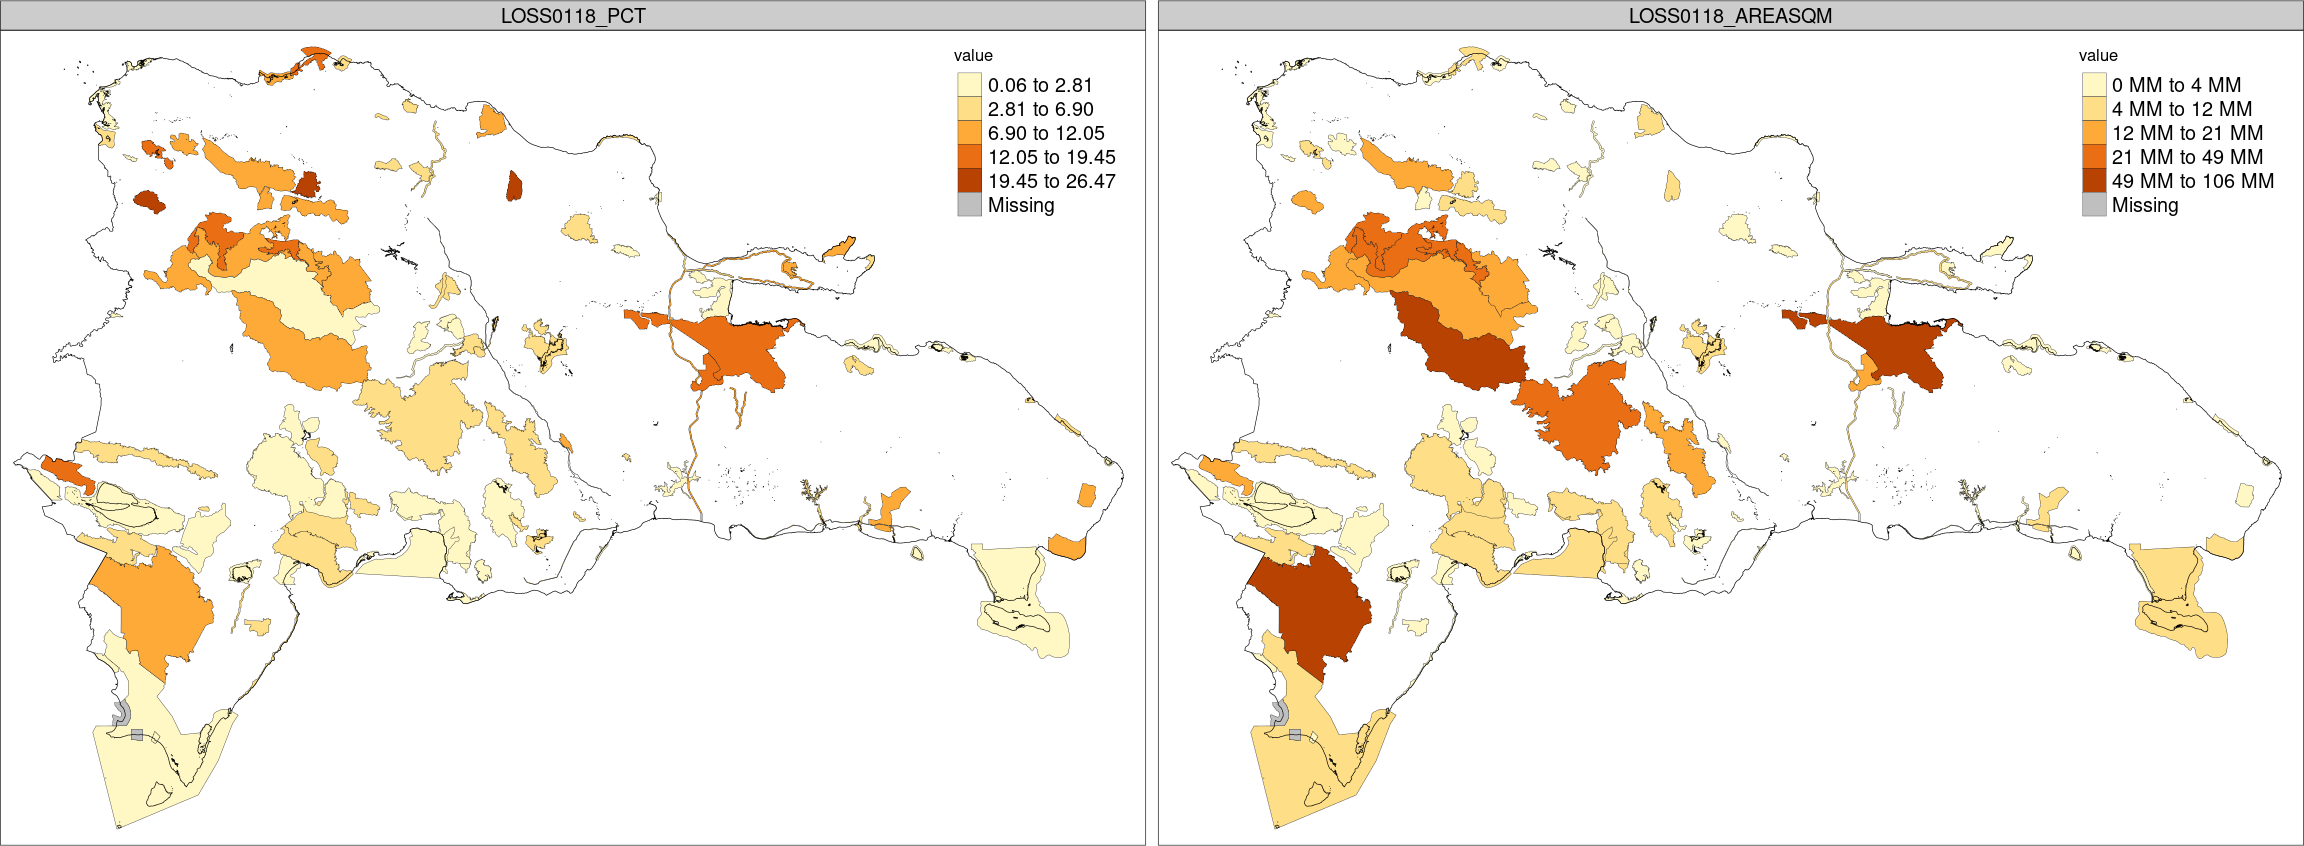
\includegraphics{img/data-download-preparation-eda/zonal-pa-6} \end{center}

\begin{Shaded}
\begin{Highlighting}[]
\CommentTok{\# ALL sorted descending by column 2}
\FunctionTok{stripped\_table}\NormalTok{(}
\NormalTok{  pazonal }\SpecialCharTok{\%\textgreater{}\%} \FunctionTok{select}\NormalTok{(CATEGORY\_NAME, }\FunctionTok{matches}\NormalTok{(}\StringTok{\textquotesingle{}\^{}LOSS0118\textquotesingle{}}\NormalTok{)) }\SpecialCharTok{\%\textgreater{}\%} \FunctionTok{select}\NormalTok{(}\SpecialCharTok{{-}}\FunctionTok{matches}\NormalTok{(}\StringTok{\textquotesingle{}\textless{}NA\textgreater{}\textquotesingle{}}\NormalTok{)),}
  \AttributeTok{n =} \FunctionTok{nrow}\NormalTok{(pazonal),}
  \AttributeTok{long\_table =}\NormalTok{ T}
\NormalTok{)}
\end{Highlighting}
\end{Shaded}

\begin{longtable}[t]{llrr}
\toprule
  & CATEGORY\_NAME & LOSS0118\_PCT & LOSS0118\_AREASQM\\
\midrule
\endfirsthead
\multicolumn{4}{@{}l}{\textit{(continued)}}\\
\toprule
  & CATEGORY\_NAME & LOSS0118\_PCT & LOSS0118\_AREASQM\\
\midrule
\endhead

\endfoot
\bottomrule
\endlastfoot
\cellcolor{lightgray}{1} & \cellcolor{lightgray}{Reserva Forestal Cerro Chacuey} & \cellcolor{lightgray}{26.4666686} & \cellcolor{lightgray}{1.373434e+07}\\
2 & Via Panoramica Entrada de Mao & 22.6278261 & 1.230196e+07\\
\cellcolor{lightgray}{3} & \cellcolor{lightgray}{Reserva Cientifica La Salcedoa} & \cellcolor{lightgray}{21.5473066} & \cellcolor{lightgray}{8.881026e+06}\\
4 & Monumento Natural Salto de Socoa & 19.4468667 & 1.328279e+07\\
\cellcolor{lightgray}{5} & \cellcolor{lightgray}{Monumento Natural Las Caobas} & \cellcolor{lightgray}{17.8894956} & \cellcolor{lightgray}{1.886845e+07}\\
\addlinespace
6 & Parque Nacional Los Haitises & 16.7961407 & 1.060981e+08\\
\cellcolor{lightgray}{7} & \cellcolor{lightgray}{Parque Nacional La Hispaniola} & \cellcolor{lightgray}{15.8335312} & \cellcolor{lightgray}{8.680829e+06}\\
8 & Refugio de Vida Silvestre Río Chacuey & 14.8619676 & 5.762642e+06\\
\cellcolor{lightgray}{9} & \cellcolor{lightgray}{Reserva Forestal Alto Mao} & \cellcolor{lightgray}{14.5829176} & \cellcolor{lightgray}{3.064084e+07}\\
10 & Parque Nacional José del Carmen Ramírez & 12.0514154 & 9.035649e+07\\
\addlinespace
\cellcolor{lightgray}{11} & \cellcolor{lightgray}{Refugio de Vida Silvestre Cañón Río Gurabo} & \cellcolor{lightgray}{11.8174946} & \cellcolor{lightgray}{3.564134e+06}\\
12 & Parque Nacional Punta Espada & 11.5707949 & 9.515568e+06\\
\cellcolor{lightgray}{13} & \cellcolor{lightgray}{Via Panoramica Autovia Santo Domingo - Samana - Boulevar del Atlantico} & \cellcolor{lightgray}{11.5427912} & \cellcolor{lightgray}{1.192278e+07}\\
14 & Parque Nacional Nalga de Maco & 10.8284097 & 1.795879e+07\\
\cellcolor{lightgray}{15} & \cellcolor{lightgray}{Parque Nacional Cabo Cabrón} & \cellcolor{lightgray}{10.8114248} & \cellcolor{lightgray}{3.851405e+06}\\
\addlinespace
16 & Monumento Natural Hoyo Claro & 10.4508619 & 4.106759e+06\\
\cellcolor{lightgray}{17} & \cellcolor{lightgray}{Parque Nacional Manolo Tavarez Justo} & \cellcolor{lightgray}{9.8789370} & \cellcolor{lightgray}{3.474684e+07}\\
18 & Parque Nacional Sierra de Bahoruco & 9.1085863 & 9.949039e+07\\
\cellcolor{lightgray}{19} & \cellcolor{lightgray}{Reserva Forestal Las Matas} & \cellcolor{lightgray}{8.9687134} & \cellcolor{lightgray}{4.285024e+06}\\
20 & Monumento Natural Río Cumayasa y Cueva de las Maravillas & 8.4629858 & 7.511724e+06\\
\addlinespace
\cellcolor{lightgray}{21} & \cellcolor{lightgray}{Monumento Natural Salto El Limón} & \cellcolor{lightgray}{8.3638311} & \cellcolor{lightgray}{1.377940e+06}\\
22 & Reserva Forestal Alto bao & 8.1503086 & 2.140120e+07\\
\cellcolor{lightgray}{23} & \cellcolor{lightgray}{Monumento Natural Salto Grande} & \cellcolor{lightgray}{7.9794657} & \cellcolor{lightgray}{1.177706e+06}\\
24 & Parque Nacional Picky Lora & 7.8947713 & 8.863962e+06\\
\cellcolor{lightgray}{25} & \cellcolor{lightgray}{Santuario De Mamiferos Marinos Estero Hondo} & \cellcolor{lightgray}{7.8195251} & \cellcolor{lightgray}{2.544674e+06}\\
\addlinespace
26 & Reserva Forestal Loma Novillero & 7.7993952 & 1.005301e+06\\
\cellcolor{lightgray}{27} & \cellcolor{lightgray}{Reserva Forestal Río Cana} & \cellcolor{lightgray}{7.4888845} & \cellcolor{lightgray}{1.946716e+07}\\
28 & Monumento Natural Lagunas Cabarete y Goleta & 7.4869378 & 5.375732e+06\\
\cellcolor{lightgray}{29} & \cellcolor{lightgray}{Monumento Natural Salto de La Damajagua} & \cellcolor{lightgray}{6.9006781} & \cellcolor{lightgray}{3.813125e+05}\\
30 & Refugio de Vida Silvestre Monumento Natural Miguel Domingo Fuerte & 6.5638506 & 2.200773e+06\\
\addlinespace
\cellcolor{lightgray}{31} & \cellcolor{lightgray}{Via Panoramica Carretera Nagua - Sánchez} & \cellcolor{lightgray}{6.5527937} & \cellcolor{lightgray}{1.103949e+06}\\
32 & Via Panoramica Mirador del Paraíso & 6.4120055 & 1.347963e+06\\
\cellcolor{lightgray}{33} & \cellcolor{lightgray}{Parque Nacional Saltos de la Jalda} & \cellcolor{lightgray}{6.3589184} & \cellcolor{lightgray}{2.316788e+06}\\
34 & Parque Nacional Montaña La Humeadora & 5.9846313 & 1.827757e+07\\
\cellcolor{lightgray}{35} & \cellcolor{lightgray}{Monumento Natural Loma Isabel de Torres} & \cellcolor{lightgray}{5.8831353} & \cellcolor{lightgray}{9.768897e+05}\\
\addlinespace
36 & Via Panoramica Carretera Santiago - La Cumbre - Puerto Plata & 5.5960474 & 1.174054e+06\\
\cellcolor{lightgray}{37} & \cellcolor{lightgray}{Parque Nacional Valle Nuevo} & \cellcolor{lightgray}{5.3641486} & \cellcolor{lightgray}{4.860623e+07}\\
38 & Monumento Natural Cabo Samaná & 5.3621004 & 4.970983e+05\\
\cellcolor{lightgray}{39} & \cellcolor{lightgray}{Reserva Biológica Loma Charco Azul} & \cellcolor{lightgray}{5.3589984} & \cellcolor{lightgray}{9.334805e+06}\\
40 & Parque Nacional Aniana Vargas & 5.3429353 & 6.925885e+06\\
\addlinespace
\cellcolor{lightgray}{41} & \cellcolor{lightgray}{Via Panoramica Carretera Bayacanes-Jarabacoa} & \cellcolor{lightgray}{5.1178604} & \cellcolor{lightgray}{8.304956e+05}\\
42 & Monumento Natural La Tinaja & 4.9885378 & 1.472586e+06\\
\cellcolor{lightgray}{43} & \cellcolor{lightgray}{Via Panoramica Mirador del Atlántico} & \cellcolor{lightgray}{4.8032548} & \cellcolor{lightgray}{5.819625e+05}\\
44 & Reserva Cientifica Las Neblinas & 4.7686062 & 1.944454e+06\\
\cellcolor{lightgray}{45} & \cellcolor{lightgray}{Refugio de Vida Silvestre Río Soco} & \cellcolor{lightgray}{4.4230649} & \cellcolor{lightgray}{5.203307e+05}\\
\addlinespace
46 & Via Panoramica Vía Panorámica Costa Azul & 4.3664582 & 8.322460e+05\\
\cellcolor{lightgray}{47} & \cellcolor{lightgray}{Reserva Forestal Loma El 20} & \cellcolor{lightgray}{4.2928178} & \cellcolor{lightgray}{2.147130e+06}\\
48 & Via Panoramica Carretera Cabral - Polo & 4.2766019 & 4.345775e+05\\
\cellcolor{lightgray}{49} & \cellcolor{lightgray}{Refugio de Vida Silvestre Ría Maimón} & \cellcolor{lightgray}{4.2676421} & \cellcolor{lightgray}{2.060333e+05}\\
50 & Corredor Ecologico Autopista 6 de Noviembre & 4.2652112 & 1.549519e+05\\
\addlinespace
\cellcolor{lightgray}{51} & \cellcolor{lightgray}{Reserva Forestal Villarpando} & \cellcolor{lightgray}{4.2454794} & \cellcolor{lightgray}{3.377307e+06}\\
52 & Area Nacional De Recreo Guagui & 4.2107689 & 1.746368e+06\\
\cellcolor{lightgray}{53} & \cellcolor{lightgray}{Parque Nacional Máximo Gómez} & \cellcolor{lightgray}{4.2038593} & \cellcolor{lightgray}{1.778012e+06}\\
54 & Parque Nacional Sierra de Neiba & 3.8649577 & 7.072866e+06\\
\cellcolor{lightgray}{55} & \cellcolor{lightgray}{Refugio de Vida Silvestre Río Higuamo} & \cellcolor{lightgray}{3.8293304} & \cellcolor{lightgray}{7.081435e+05}\\
\addlinespace
56 & Monumento Natural Las Marías & 3.8115492 & 1.716999e+05\\
\cellcolor{lightgray}{57} & \cellcolor{lightgray}{Reserva Cientifica Loma Quita Espuela} & \cellcolor{lightgray}{3.4800012} & \cellcolor{lightgray}{2.635633e+06}\\
58 & Refugio de Vida Silvestre Bahia de Luperón & 3.2791403 & 6.126976e+05\\
\cellcolor{lightgray}{59} & \cellcolor{lightgray}{Reserva Forestal Barrero} & \cellcolor{lightgray}{3.2605838} & \cellcolor{lightgray}{1.012874e+07}\\
60 & Parque Nacional Sierra Martín García & 3.2280569 & 8.441457e+06\\
\addlinespace
\cellcolor{lightgray}{61} & \cellcolor{lightgray}{Monumento Natural Reserva Antropológica Cuevas de Borbón o del Pomier} & \cellcolor{lightgray}{3.1927358} & \cellcolor{lightgray}{1.603398e+05}\\
62 & Monumento Natural Diego de Ocampo & 3.1409661 & 7.960324e+05\\
\cellcolor{lightgray}{63} & \cellcolor{lightgray}{Corredor Ecologico Autopista Juan Bosch} & \cellcolor{lightgray}{3.1337140} & \cellcolor{lightgray}{1.738543e+05}\\
64 & Reserva Biológica Sierra Prieta & 3.0743741 & 1.229764e+05\\
\cellcolor{lightgray}{65} & \cellcolor{lightgray}{Refugio de Vida Silvestre Laguna Saladilla} & \cellcolor{lightgray}{3.0472813} & \cellcolor{lightgray}{9.481367e+05}\\
\addlinespace
66 & Reserva Cientifica Loma Barbacoa & 2.9683306 & 4.068947e+05\\
\cellcolor{lightgray}{67} & \cellcolor{lightgray}{Monumento Natural Saltos de Jima} & \cellcolor{lightgray}{2.9440900} & \cellcolor{lightgray}{5.465493e+05}\\
68 & Parque Nacional Luis Quin & 2.8069861 & 5.538027e+06\\
\cellcolor{lightgray}{69} & \cellcolor{lightgray}{Via Panoramica Carretera El Abanico - Constanza} & \cellcolor{lightgray}{2.7128399} & \cellcolor{lightgray}{6.170540e+05}\\
70 & Monumento Natural Cerro de San Francisco & 2.6310981 & 1.058943e+05\\
\addlinespace
\cellcolor{lightgray}{71} & \cellcolor{lightgray}{Parque Nacional Baiguate} & \cellcolor{lightgray}{2.5817049} & \cellcolor{lightgray}{1.353512e+06}\\
72 & Refugio de Vida Silvestre Laguna Cabral o Rincón & 2.5207767 & 1.412513e+06\\
\cellcolor{lightgray}{73} & \cellcolor{lightgray}{Reserva Forestal Guanito} & \cellcolor{lightgray}{2.2209652} & \cellcolor{lightgray}{1.531254e+06}\\
74 & Parque Nacional Armando Bermúdez & 2.1521028 & 1.727170e+07\\
\cellcolor{lightgray}{75} & \cellcolor{lightgray}{Corredor Ecologico Autopista Duarte} & \cellcolor{lightgray}{2.0818581} & \cellcolor{lightgray}{2.158105e+05}\\
\addlinespace
76 & Reserva Forestal Hatillo & 1.9647072 & 6.270945e+06\\
\cellcolor{lightgray}{77} & \cellcolor{lightgray}{Parque Nacional La Gran Sabana} & \cellcolor{lightgray}{1.9438134} & \cellcolor{lightgray}{4.268147e+06}\\
78 & Parque Nacional Humedales del Ozama & 1.9053804 & 8.844452e+05\\
\cellcolor{lightgray}{79} & \cellcolor{lightgray}{Reserva Cientifica Loma Guaconejo} & \cellcolor{lightgray}{1.8671873} & \cellcolor{lightgray}{4.363857e+05}\\
80 & Parque Nacional Manglares del Bajo Yuna & 1.7645273 & 2.137810e+06\\
\addlinespace
\cellcolor{lightgray}{81} & \cellcolor{lightgray}{Reserva Forestal Arroyo Cano} & \cellcolor{lightgray}{1.4002585} & \cellcolor{lightgray}{3.346449e+05}\\
82 & Reserva Cientifica Ébano Verde & 1.3922027 & 4.162576e+05\\
\cellcolor{lightgray}{83} & \cellcolor{lightgray}{Reserva Forestal Cayuco} & \cellcolor{lightgray}{1.3722628} & \cellcolor{lightgray}{6.914752e+04}\\
84 & Parque Nacional El Morro & 1.1670811 & 2.143125e+05\\
\cellcolor{lightgray}{85} & \cellcolor{lightgray}{Refugio de Vida Silvestre Lagunas Redonda y Limón} & \cellcolor{lightgray}{1.1499667} & \cellcolor{lightgray}{3.053692e+05}\\
\addlinespace
86 & Refugio de Vida Silvestre Humedales del Bajo Yaque del Sur & 1.1086223 & 6.481264e+05\\
\cellcolor{lightgray}{87} & \cellcolor{lightgray}{Parque Nacional Cotubanamá (Del Este)} & \cellcolor{lightgray}{1.0818280} & \cellcolor{lightgray}{8.615735e+06}\\
88 & Parque Nacional Francisco Alberto Caamaño Deñó & 1.0273068 & 6.035530e+06\\
\cellcolor{lightgray}{89} & \cellcolor{lightgray}{Parque Nacional Anacaona} & \cellcolor{lightgray}{0.8662760} & \cellcolor{lightgray}{4.668627e+06}\\
90 & Parque Nacional Manglares de Estero Balsa & 0.8484612 & 4.797743e+05\\
\addlinespace
\cellcolor{lightgray}{91} & \cellcolor{lightgray}{Monumento Natural Salto de Jimenoa} & \cellcolor{lightgray}{0.8439175} & \cellcolor{lightgray}{1.471035e+05}\\
92 & Reserva Forestal Cabeza de Toro & 0.7569748 & 2.843338e+06\\
\cellcolor{lightgray}{93} & \cellcolor{lightgray}{Parque Nacional Lago Enriquillo e Isla Cabritos} & \cellcolor{lightgray}{0.6845694} & \cellcolor{lightgray}{2.772054e+06}\\
94 & Area Nacional De Recreo Boca de Nigua & 0.6713110 & 3.903465e+04\\
\cellcolor{lightgray}{95} & \cellcolor{lightgray}{Refugio de Vida Silvestre La Gran Laguna o Perucho} & \cellcolor{lightgray}{0.6343772} & \cellcolor{lightgray}{4.643403e+04}\\
\addlinespace
96 & Refugio de Vida Silvestre Manglar de la Jina & 0.4690262 & 2.479481e+05\\
\cellcolor{lightgray}{97} & \cellcolor{lightgray}{Monumento Natural Las Dunas de las Calderas} & \cellcolor{lightgray}{0.4461092} & \cellcolor{lightgray}{7.797633e+04}\\
98 & Refugio de Vida Silvestre Manglares de Puerto Viejo & 0.4427118 & 4.929034e+04\\
\cellcolor{lightgray}{99} & \cellcolor{lightgray}{Reserva Forestal Cerro de Bocanigua} & \cellcolor{lightgray}{0.3878312} & \cellcolor{lightgray}{1.132792e+05}\\
100 & Parque Nacional Jaragua & 0.3557469 & 5.460767e+06\\
\addlinespace
\cellcolor{lightgray}{101} & \cellcolor{lightgray}{Monumento Natural Los Cacheos} & \cellcolor{lightgray}{0.2519722} & \cellcolor{lightgray}{1.405244e+05}\\
102 & Monumento Natural Isla Catalina & 0.2263980 & 3.676560e+04\\
\cellcolor{lightgray}{103} & \cellcolor{lightgray}{Area Nacional De Recreo Playa de Cabo Rojo - Pedernales} & \cellcolor{lightgray}{0.1847187} & \cellcolor{lightgray}{3.235779e+04}\\
104 & Refugio de Vida Silvestre Lagunas de Bávaro y El Caletón & 0.1494940 & 9.567537e+03\\
\cellcolor{lightgray}{105} & \cellcolor{lightgray}{Area Nacional De Recreo Guaraguao - Punta Catuano} & \cellcolor{lightgray}{0.1465114} & \cellcolor{lightgray}{2.724377e+04}\\
\addlinespace
106 & Area Nacional De Recreo Playa Blanca & 0.0551998 & 3.677716e+03\\
\cellcolor{lightgray}{107} & \cellcolor{lightgray}{Area Nacional De Recreo Bahía de las Águilas} & \cellcolor{lightgray}{NA} & \cellcolor{lightgray}{NA}\\
108 & Area Nacional De Recreo Playa Larga & NA & NA\\*
\end{longtable}

\begin{Shaded}
\begin{Highlighting}[]
\CommentTok{\# ALL sorted descending by column 3}
\FunctionTok{stripped\_table}\NormalTok{(}
\NormalTok{  pazonal }\SpecialCharTok{\%\textgreater{}\%} \FunctionTok{select}\NormalTok{(CATEGORY\_NAME, }\FunctionTok{matches}\NormalTok{(}\StringTok{\textquotesingle{}\^{}LOSS0118\textquotesingle{}}\NormalTok{)) }\SpecialCharTok{\%\textgreater{}\%} \FunctionTok{select}\NormalTok{(}\SpecialCharTok{{-}}\FunctionTok{matches}\NormalTok{(}\StringTok{\textquotesingle{}\textless{}NA\textgreater{}\textquotesingle{}}\NormalTok{)),}
  \AttributeTok{n =} \FunctionTok{nrow}\NormalTok{(pazonal),}
  \AttributeTok{order\_col =} \DecValTok{3}\NormalTok{,}
  \AttributeTok{long\_table =}\NormalTok{ T}
\NormalTok{)}
\end{Highlighting}
\end{Shaded}

\begin{longtable}[t]{llrr}
\toprule
  & CATEGORY\_NAME & LOSS0118\_PCT & LOSS0118\_AREASQM\\
\midrule
\endfirsthead
\multicolumn{4}{@{}l}{\textit{(continued)}}\\
\toprule
  & CATEGORY\_NAME & LOSS0118\_PCT & LOSS0118\_AREASQM\\
\midrule
\endhead

\endfoot
\bottomrule
\endlastfoot
\cellcolor{lightgray}{1} & \cellcolor{lightgray}{Parque Nacional Los Haitises} & \cellcolor{lightgray}{16.7961407} & \cellcolor{lightgray}{1.060981e+08}\\
2 & Parque Nacional Sierra de Bahoruco & 9.1085863 & 9.949039e+07\\
\cellcolor{lightgray}{3} & \cellcolor{lightgray}{Parque Nacional José del Carmen Ramírez} & \cellcolor{lightgray}{12.0514154} & \cellcolor{lightgray}{9.035649e+07}\\
4 & Parque Nacional Valle Nuevo & 5.3641486 & 4.860623e+07\\
\cellcolor{lightgray}{5} & \cellcolor{lightgray}{Parque Nacional Manolo Tavarez Justo} & \cellcolor{lightgray}{9.8789370} & \cellcolor{lightgray}{3.474684e+07}\\
\addlinespace
6 & Reserva Forestal Alto Mao & 14.5829176 & 3.064084e+07\\
\cellcolor{lightgray}{7} & \cellcolor{lightgray}{Reserva Forestal Alto bao} & \cellcolor{lightgray}{8.1503086} & \cellcolor{lightgray}{2.140120e+07}\\
8 & Reserva Forestal Río Cana & 7.4888845 & 1.946716e+07\\
\cellcolor{lightgray}{9} & \cellcolor{lightgray}{Monumento Natural Las Caobas} & \cellcolor{lightgray}{17.8894956} & \cellcolor{lightgray}{1.886845e+07}\\
10 & Parque Nacional Montaña La Humeadora & 5.9846313 & 1.827757e+07\\
\addlinespace
\cellcolor{lightgray}{11} & \cellcolor{lightgray}{Parque Nacional Nalga de Maco} & \cellcolor{lightgray}{10.8284097} & \cellcolor{lightgray}{1.795879e+07}\\
12 & Parque Nacional Armando Bermúdez & 2.1521028 & 1.727170e+07\\
\cellcolor{lightgray}{13} & \cellcolor{lightgray}{Reserva Forestal Cerro Chacuey} & \cellcolor{lightgray}{26.4666686} & \cellcolor{lightgray}{1.373434e+07}\\
14 & Monumento Natural Salto de Socoa & 19.4468667 & 1.328279e+07\\
\cellcolor{lightgray}{15} & \cellcolor{lightgray}{Via Panoramica Entrada de Mao} & \cellcolor{lightgray}{22.6278261} & \cellcolor{lightgray}{1.230196e+07}\\
\addlinespace
16 & Via Panoramica Autovia Santo Domingo - Samana - Boulevar del Atlantico & 11.5427912 & 1.192278e+07\\
\cellcolor{lightgray}{17} & \cellcolor{lightgray}{Reserva Forestal Barrero} & \cellcolor{lightgray}{3.2605838} & \cellcolor{lightgray}{1.012874e+07}\\
18 & Parque Nacional Punta Espada & 11.5707949 & 9.515568e+06\\
\cellcolor{lightgray}{19} & \cellcolor{lightgray}{Reserva Biológica Loma Charco Azul} & \cellcolor{lightgray}{5.3589984} & \cellcolor{lightgray}{9.334805e+06}\\
20 & Reserva Cientifica La Salcedoa & 21.5473066 & 8.881026e+06\\
\addlinespace
\cellcolor{lightgray}{21} & \cellcolor{lightgray}{Parque Nacional Picky Lora} & \cellcolor{lightgray}{7.8947713} & \cellcolor{lightgray}{8.863962e+06}\\
22 & Parque Nacional La Hispaniola & 15.8335312 & 8.680829e+06\\
\cellcolor{lightgray}{23} & \cellcolor{lightgray}{Parque Nacional Cotubanamá (Del Este)} & \cellcolor{lightgray}{1.0818280} & \cellcolor{lightgray}{8.615735e+06}\\
24 & Parque Nacional Sierra Martín García & 3.2280569 & 8.441457e+06\\
\cellcolor{lightgray}{25} & \cellcolor{lightgray}{Monumento Natural Río Cumayasa y Cueva de las Maravillas} & \cellcolor{lightgray}{8.4629858} & \cellcolor{lightgray}{7.511724e+06}\\
\addlinespace
26 & Parque Nacional Sierra de Neiba & 3.8649577 & 7.072866e+06\\
\cellcolor{lightgray}{27} & \cellcolor{lightgray}{Parque Nacional Aniana Vargas} & \cellcolor{lightgray}{5.3429353} & \cellcolor{lightgray}{6.925885e+06}\\
28 & Reserva Forestal Hatillo & 1.9647072 & 6.270945e+06\\
\cellcolor{lightgray}{29} & \cellcolor{lightgray}{Parque Nacional Francisco Alberto Caamaño Deñó} & \cellcolor{lightgray}{1.0273068} & \cellcolor{lightgray}{6.035530e+06}\\
30 & Refugio de Vida Silvestre Río Chacuey & 14.8619676 & 5.762642e+06\\
\addlinespace
\cellcolor{lightgray}{31} & \cellcolor{lightgray}{Parque Nacional Luis Quin} & \cellcolor{lightgray}{2.8069861} & \cellcolor{lightgray}{5.538027e+06}\\
32 & Parque Nacional Jaragua & 0.3557469 & 5.460767e+06\\
\cellcolor{lightgray}{33} & \cellcolor{lightgray}{Monumento Natural Lagunas Cabarete y Goleta} & \cellcolor{lightgray}{7.4869378} & \cellcolor{lightgray}{5.375732e+06}\\
34 & Parque Nacional Anacaona & 0.8662760 & 4.668627e+06\\
\cellcolor{lightgray}{35} & \cellcolor{lightgray}{Reserva Forestal Las Matas} & \cellcolor{lightgray}{8.9687134} & \cellcolor{lightgray}{4.285024e+06}\\
\addlinespace
36 & Parque Nacional La Gran Sabana & 1.9438134 & 4.268147e+06\\
\cellcolor{lightgray}{37} & \cellcolor{lightgray}{Monumento Natural Hoyo Claro} & \cellcolor{lightgray}{10.4508619} & \cellcolor{lightgray}{4.106759e+06}\\
38 & Parque Nacional Cabo Cabrón & 10.8114248 & 3.851405e+06\\
\cellcolor{lightgray}{39} & \cellcolor{lightgray}{Refugio de Vida Silvestre Cañón Río Gurabo} & \cellcolor{lightgray}{11.8174946} & \cellcolor{lightgray}{3.564134e+06}\\
40 & Reserva Forestal Villarpando & 4.2454794 & 3.377307e+06\\
\addlinespace
\cellcolor{lightgray}{41} & \cellcolor{lightgray}{Reserva Forestal Cabeza de Toro} & \cellcolor{lightgray}{0.7569748} & \cellcolor{lightgray}{2.843338e+06}\\
42 & Parque Nacional Lago Enriquillo e Isla Cabritos & 0.6845694 & 2.772054e+06\\
\cellcolor{lightgray}{43} & \cellcolor{lightgray}{Reserva Cientifica Loma Quita Espuela} & \cellcolor{lightgray}{3.4800012} & \cellcolor{lightgray}{2.635633e+06}\\
44 & Santuario De Mamiferos Marinos Estero Hondo & 7.8195251 & 2.544674e+06\\
\cellcolor{lightgray}{45} & \cellcolor{lightgray}{Parque Nacional Saltos de la Jalda} & \cellcolor{lightgray}{6.3589184} & \cellcolor{lightgray}{2.316788e+06}\\
\addlinespace
46 & Refugio de Vida Silvestre Monumento Natural Miguel Domingo Fuerte & 6.5638506 & 2.200773e+06\\
\cellcolor{lightgray}{47} & \cellcolor{lightgray}{Reserva Forestal Loma El 20} & \cellcolor{lightgray}{4.2928178} & \cellcolor{lightgray}{2.147130e+06}\\
48 & Parque Nacional Manglares del Bajo Yuna & 1.7645273 & 2.137810e+06\\
\cellcolor{lightgray}{49} & \cellcolor{lightgray}{Reserva Cientifica Las Neblinas} & \cellcolor{lightgray}{4.7686062} & \cellcolor{lightgray}{1.944454e+06}\\
50 & Parque Nacional Máximo Gómez & 4.2038593 & 1.778012e+06\\
\addlinespace
\cellcolor{lightgray}{51} & \cellcolor{lightgray}{Area Nacional De Recreo Guagui} & \cellcolor{lightgray}{4.2107689} & \cellcolor{lightgray}{1.746368e+06}\\
52 & Reserva Forestal Guanito & 2.2209652 & 1.531254e+06\\
\cellcolor{lightgray}{53} & \cellcolor{lightgray}{Monumento Natural La Tinaja} & \cellcolor{lightgray}{4.9885378} & \cellcolor{lightgray}{1.472586e+06}\\
54 & Refugio de Vida Silvestre Laguna Cabral o Rincón & 2.5207767 & 1.412513e+06\\
\cellcolor{lightgray}{55} & \cellcolor{lightgray}{Monumento Natural Salto El Limón} & \cellcolor{lightgray}{8.3638311} & \cellcolor{lightgray}{1.377940e+06}\\
\addlinespace
56 & Parque Nacional Baiguate & 2.5817049 & 1.353512e+06\\
\cellcolor{lightgray}{57} & \cellcolor{lightgray}{Via Panoramica Mirador del Paraíso} & \cellcolor{lightgray}{6.4120055} & \cellcolor{lightgray}{1.347963e+06}\\
58 & Monumento Natural Salto Grande & 7.9794657 & 1.177706e+06\\
\cellcolor{lightgray}{59} & \cellcolor{lightgray}{Via Panoramica Carretera Santiago - La Cumbre - Puerto Plata} & \cellcolor{lightgray}{5.5960474} & \cellcolor{lightgray}{1.174054e+06}\\
60 & Via Panoramica Carretera Nagua - Sánchez & 6.5527937 & 1.103949e+06\\
\addlinespace
\cellcolor{lightgray}{61} & \cellcolor{lightgray}{Reserva Forestal Loma Novillero} & \cellcolor{lightgray}{7.7993952} & \cellcolor{lightgray}{1.005301e+06}\\
62 & Monumento Natural Loma Isabel de Torres & 5.8831353 & 9.768897e+05\\
\cellcolor{lightgray}{63} & \cellcolor{lightgray}{Refugio de Vida Silvestre Laguna Saladilla} & \cellcolor{lightgray}{3.0472813} & \cellcolor{lightgray}{9.481367e+05}\\
64 & Parque Nacional Humedales del Ozama & 1.9053804 & 8.844452e+05\\
\cellcolor{lightgray}{65} & \cellcolor{lightgray}{Via Panoramica Vía Panorámica Costa Azul} & \cellcolor{lightgray}{4.3664582} & \cellcolor{lightgray}{8.322460e+05}\\
\addlinespace
66 & Via Panoramica Carretera Bayacanes-Jarabacoa & 5.1178604 & 8.304956e+05\\
\cellcolor{lightgray}{67} & \cellcolor{lightgray}{Monumento Natural Diego de Ocampo} & \cellcolor{lightgray}{3.1409661} & \cellcolor{lightgray}{7.960324e+05}\\
68 & Refugio de Vida Silvestre Río Higuamo & 3.8293304 & 7.081435e+05\\
\cellcolor{lightgray}{69} & \cellcolor{lightgray}{Refugio de Vida Silvestre Humedales del Bajo Yaque del Sur} & \cellcolor{lightgray}{1.1086223} & \cellcolor{lightgray}{6.481264e+05}\\
70 & Via Panoramica Carretera El Abanico - Constanza & 2.7128399 & 6.170540e+05\\
\addlinespace
\cellcolor{lightgray}{71} & \cellcolor{lightgray}{Refugio de Vida Silvestre Bahia de Luperón} & \cellcolor{lightgray}{3.2791403} & \cellcolor{lightgray}{6.126976e+05}\\
72 & Via Panoramica Mirador del Atlántico & 4.8032548 & 5.819625e+05\\
\cellcolor{lightgray}{73} & \cellcolor{lightgray}{Monumento Natural Saltos de Jima} & \cellcolor{lightgray}{2.9440900} & \cellcolor{lightgray}{5.465493e+05}\\
74 & Refugio de Vida Silvestre Río Soco & 4.4230649 & 5.203307e+05\\
\cellcolor{lightgray}{75} & \cellcolor{lightgray}{Monumento Natural Cabo Samaná} & \cellcolor{lightgray}{5.3621004} & \cellcolor{lightgray}{4.970983e+05}\\
\addlinespace
76 & Parque Nacional Manglares de Estero Balsa & 0.8484612 & 4.797743e+05\\
\cellcolor{lightgray}{77} & \cellcolor{lightgray}{Reserva Cientifica Loma Guaconejo} & \cellcolor{lightgray}{1.8671873} & \cellcolor{lightgray}{4.363857e+05}\\
78 & Via Panoramica Carretera Cabral - Polo & 4.2766019 & 4.345775e+05\\
\cellcolor{lightgray}{79} & \cellcolor{lightgray}{Reserva Cientifica Ébano Verde} & \cellcolor{lightgray}{1.3922027} & \cellcolor{lightgray}{4.162576e+05}\\
80 & Reserva Cientifica Loma Barbacoa & 2.9683306 & 4.068947e+05\\
\addlinespace
\cellcolor{lightgray}{81} & \cellcolor{lightgray}{Monumento Natural Salto de La Damajagua} & \cellcolor{lightgray}{6.9006781} & \cellcolor{lightgray}{3.813125e+05}\\
82 & Reserva Forestal Arroyo Cano & 1.4002585 & 3.346449e+05\\
\cellcolor{lightgray}{83} & \cellcolor{lightgray}{Refugio de Vida Silvestre Lagunas Redonda y Limón} & \cellcolor{lightgray}{1.1499667} & \cellcolor{lightgray}{3.053692e+05}\\
84 & Refugio de Vida Silvestre Manglar de la Jina & 0.4690262 & 2.479481e+05\\
\cellcolor{lightgray}{85} & \cellcolor{lightgray}{Corredor Ecologico Autopista Duarte} & \cellcolor{lightgray}{2.0818581} & \cellcolor{lightgray}{2.158105e+05}\\
\addlinespace
86 & Parque Nacional El Morro & 1.1670811 & 2.143125e+05\\
\cellcolor{lightgray}{87} & \cellcolor{lightgray}{Refugio de Vida Silvestre Ría Maimón} & \cellcolor{lightgray}{4.2676421} & \cellcolor{lightgray}{2.060333e+05}\\
88 & Corredor Ecologico Autopista Juan Bosch & 3.1337140 & 1.738543e+05\\
\cellcolor{lightgray}{89} & \cellcolor{lightgray}{Monumento Natural Las Marías} & \cellcolor{lightgray}{3.8115492} & \cellcolor{lightgray}{1.716999e+05}\\
90 & Monumento Natural Reserva Antropológica Cuevas de Borbón o del Pomier & 3.1927358 & 1.603398e+05\\
\addlinespace
\cellcolor{lightgray}{91} & \cellcolor{lightgray}{Corredor Ecologico Autopista 6 de Noviembre} & \cellcolor{lightgray}{4.2652112} & \cellcolor{lightgray}{1.549519e+05}\\
92 & Monumento Natural Salto de Jimenoa & 0.8439175 & 1.471035e+05\\
\cellcolor{lightgray}{93} & \cellcolor{lightgray}{Monumento Natural Los Cacheos} & \cellcolor{lightgray}{0.2519722} & \cellcolor{lightgray}{1.405244e+05}\\
94 & Reserva Biológica Sierra Prieta & 3.0743741 & 1.229764e+05\\
\cellcolor{lightgray}{95} & \cellcolor{lightgray}{Reserva Forestal Cerro de Bocanigua} & \cellcolor{lightgray}{0.3878312} & \cellcolor{lightgray}{1.132792e+05}\\
\addlinespace
96 & Monumento Natural Cerro de San Francisco & 2.6310981 & 1.058943e+05\\
\cellcolor{lightgray}{97} & \cellcolor{lightgray}{Monumento Natural Las Dunas de las Calderas} & \cellcolor{lightgray}{0.4461092} & \cellcolor{lightgray}{7.797633e+04}\\
98 & Reserva Forestal Cayuco & 1.3722628 & 6.914752e+04\\
\cellcolor{lightgray}{99} & \cellcolor{lightgray}{Refugio de Vida Silvestre Manglares de Puerto Viejo} & \cellcolor{lightgray}{0.4427118} & \cellcolor{lightgray}{4.929034e+04}\\
100 & Refugio de Vida Silvestre La Gran Laguna o Perucho & 0.6343772 & 4.643403e+04\\
\addlinespace
\cellcolor{lightgray}{101} & \cellcolor{lightgray}{Area Nacional De Recreo Boca de Nigua} & \cellcolor{lightgray}{0.6713110} & \cellcolor{lightgray}{3.903465e+04}\\
102 & Monumento Natural Isla Catalina & 0.2263980 & 3.676560e+04\\
\cellcolor{lightgray}{103} & \cellcolor{lightgray}{Area Nacional De Recreo Playa de Cabo Rojo - Pedernales} & \cellcolor{lightgray}{0.1847187} & \cellcolor{lightgray}{3.235779e+04}\\
104 & Area Nacional De Recreo Guaraguao - Punta Catuano & 0.1465114 & 2.724377e+04\\
\cellcolor{lightgray}{105} & \cellcolor{lightgray}{Refugio de Vida Silvestre Lagunas de Bávaro y El Caletón} & \cellcolor{lightgray}{0.1494940} & \cellcolor{lightgray}{9.567537e+03}\\
\addlinespace
106 & Area Nacional De Recreo Playa Blanca & 0.0551998 & 3.677716e+03\\
\cellcolor{lightgray}{107} & \cellcolor{lightgray}{Area Nacional De Recreo Bahía de las Águilas} & \cellcolor{lightgray}{NA} & \cellcolor{lightgray}{NA}\\
108 & Area Nacional De Recreo Playa Larga & NA & NA\\*
\end{longtable}

\begin{Shaded}
\begin{Highlighting}[]

\CommentTok{\# Total loss 2012{-}2018}
\NormalTok{pazonal }\SpecialCharTok{\%\textgreater{}\%} \FunctionTok{select}\NormalTok{(}\FunctionTok{matches}\NormalTok{(}\StringTok{\textquotesingle{}\^{}LOSS1218\textquotesingle{}}\NormalTok{)) }\SpecialCharTok{\%\textgreater{}\%} \FunctionTok{select}\NormalTok{(}\SpecialCharTok{{-}}\FunctionTok{matches}\NormalTok{(}\StringTok{\textquotesingle{}\textless{}NA\textgreater{}\textquotesingle{}}\NormalTok{)) }\SpecialCharTok{\%\textgreater{}\%} 
  \FunctionTok{gather}\NormalTok{(variable, value, }\SpecialCharTok{{-}}\NormalTok{geom) }\SpecialCharTok{\%\textgreater{}\%}
  \FunctionTok{mutate}\NormalTok{(}\AttributeTok{variable =} \FunctionTok{factor}\NormalTok{(variable, }\AttributeTok{levels =} \FunctionTok{unique}\NormalTok{(variable))) }\SpecialCharTok{\%\textgreater{}\%} 
  \FunctionTok{tm\_shape}\NormalTok{() }\SpecialCharTok{+}
  \FunctionTok{tm\_fill}\NormalTok{(}\AttributeTok{col=}\StringTok{\textquotesingle{}value\textquotesingle{}}\NormalTok{, }\AttributeTok{palette =} \StringTok{"YlOrBr"}\NormalTok{, }\AttributeTok{size =} \FloatTok{0.1}\NormalTok{, }\AttributeTok{style =} \StringTok{\textquotesingle{}jenks\textquotesingle{}}\NormalTok{) }\SpecialCharTok{+}
  \FunctionTok{tm\_borders}\NormalTok{(}\AttributeTok{col =} \StringTok{\textquotesingle{}grey15\textquotesingle{}}\NormalTok{, }\AttributeTok{lwd =} \FloatTok{0.3}\NormalTok{) }\SpecialCharTok{+}
  \FunctionTok{tm\_facets}\NormalTok{(}\AttributeTok{by =} \StringTok{"variable"}\NormalTok{, }\AttributeTok{ncol =} \DecValTok{2}\NormalTok{, }\AttributeTok{nrow =} \DecValTok{1}\NormalTok{, }\AttributeTok{free.coords =} \ConstantTok{FALSE}\NormalTok{, }\AttributeTok{free.scales =} \ConstantTok{TRUE}\NormalTok{) }\SpecialCharTok{+}
  \FunctionTok{tm\_layout}\NormalTok{(}\AttributeTok{panel.label.size =} \DecValTok{1}\NormalTok{, }\AttributeTok{legend.title.size =} \DecValTok{1}\NormalTok{, }\AttributeTok{legend.text.size =} \DecValTok{1}\NormalTok{) }\SpecialCharTok{+} 
  \FunctionTok{tm\_shape}\NormalTok{(}\AttributeTok{shp =}\NormalTok{ cline) }\SpecialCharTok{+} \FunctionTok{tm\_borders}\NormalTok{(}\AttributeTok{col =} \StringTok{\textquotesingle{}black\textquotesingle{}}\NormalTok{, }\AttributeTok{lwd =} \FloatTok{0.5}\NormalTok{)}
\end{Highlighting}
\end{Shaded}

\begin{center}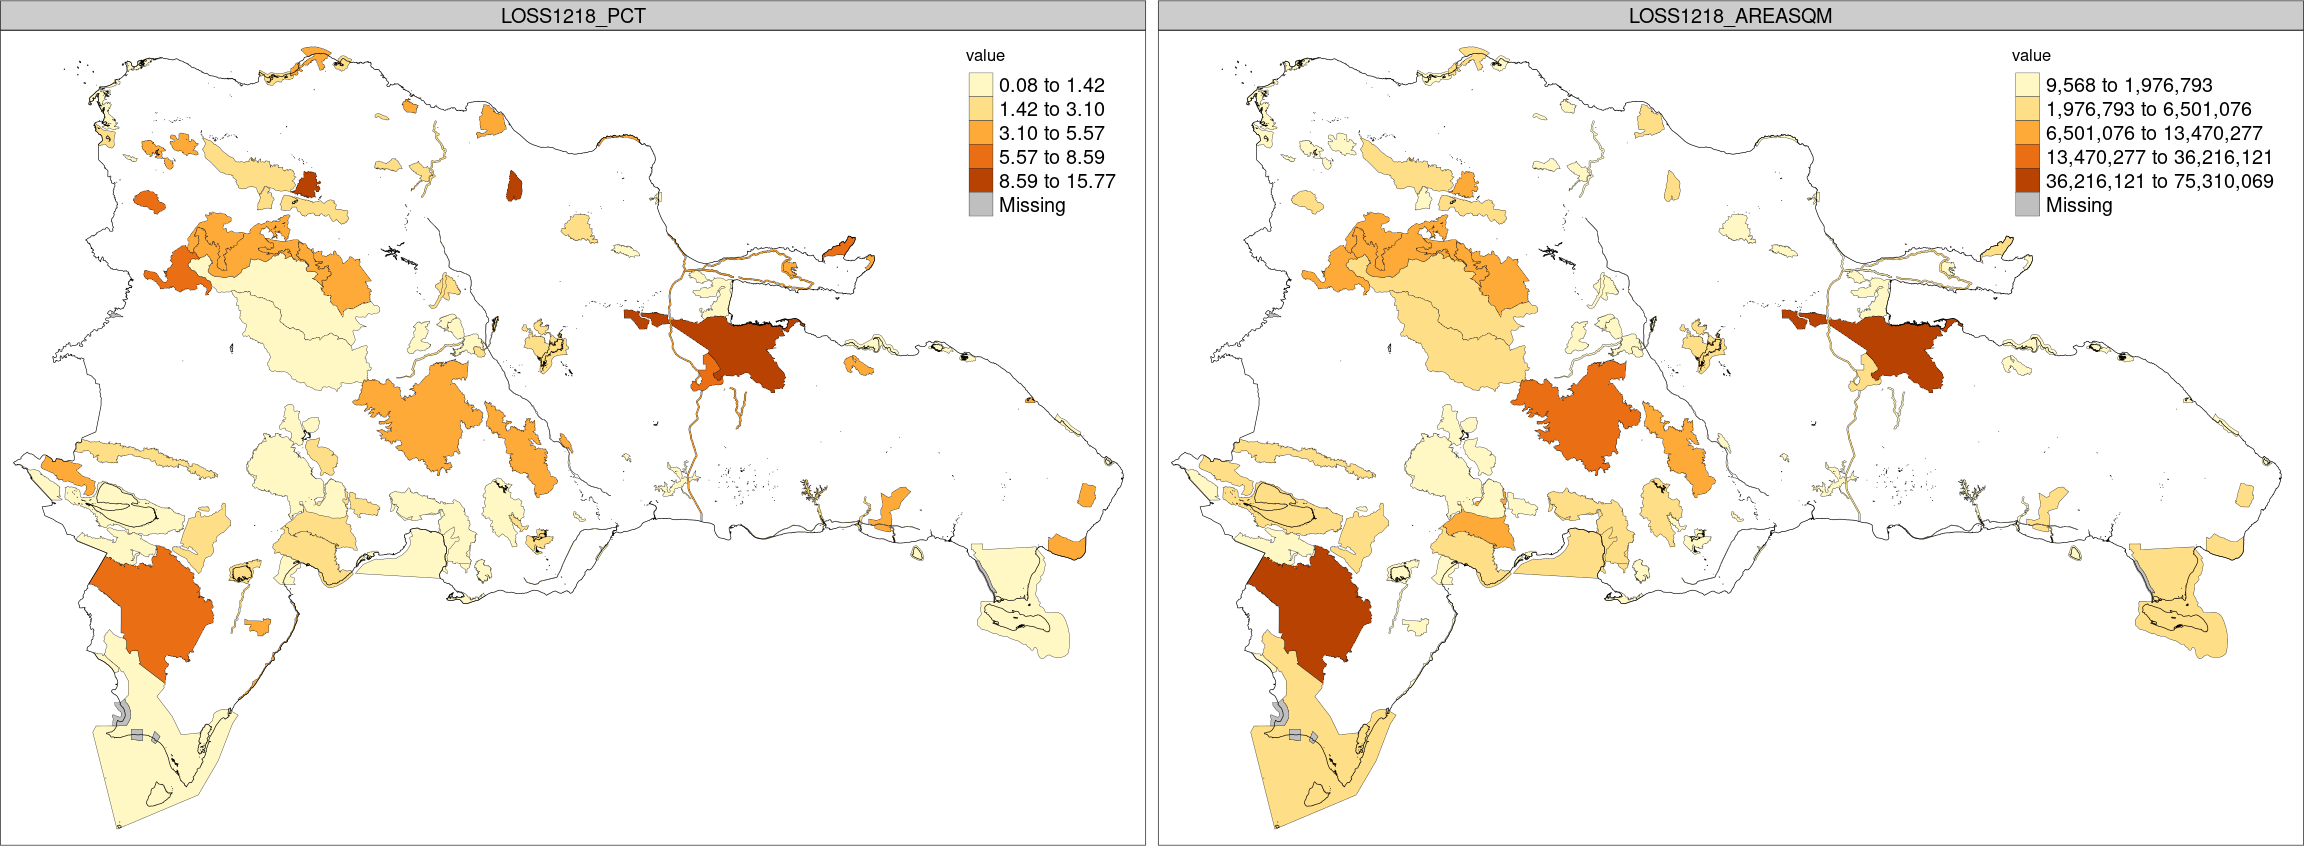
\includegraphics{img/data-download-preparation-eda/zonal-pa-7} \end{center}

\begin{Shaded}
\begin{Highlighting}[]
\CommentTok{\# Top twenty sorted descending by column 2}
\FunctionTok{stripped\_table}\NormalTok{(pazonal }\SpecialCharTok{\%\textgreater{}\%} \FunctionTok{select}\NormalTok{(CATEGORY\_NAME, }\FunctionTok{matches}\NormalTok{(}\StringTok{\textquotesingle{}\^{}LOSS1218\textquotesingle{}}\NormalTok{)) }\SpecialCharTok{\%\textgreater{}\%} \FunctionTok{select}\NormalTok{(}\SpecialCharTok{{-}}\FunctionTok{matches}\NormalTok{(}\StringTok{\textquotesingle{}\textless{}NA\textgreater{}\textquotesingle{}}\NormalTok{)))}
\end{Highlighting}
\end{Shaded}

\begin{table}[H]
\centering
\begin{tabular}[t]{llrr}
\toprule
  & CATEGORY\_NAME & LOSS1218\_PCT & LOSS1218\_AREASQM\\
\midrule
\cellcolor{lightgray}{1} & \cellcolor{lightgray}{Reserva Cientifica La Salcedoa} & \cellcolor{lightgray}{15.773028} & \cellcolor{lightgray}{6501076.2}\\
2 & Via Panoramica Entrada de Mao & 14.178246 & 7708217.1\\
\cellcolor{lightgray}{3} & \cellcolor{lightgray}{Parque Nacional Los Haitises} & \cellcolor{lightgray}{11.668154} & \cellcolor{lightgray}{73705545.1}\\
4 & Reserva Forestal Cerro Chacuey & 8.593019 & 4459171.5\\
\cellcolor{lightgray}{5} & \cellcolor{lightgray}{Monumento Natural Salto de Socoa} & \cellcolor{lightgray}{8.132287} & \cellcolor{lightgray}{5554593.8}\\
\addlinespace
6 & Parque Nacional Cabo Cabrón & 7.604139 & 2708858.5\\
\cellcolor{lightgray}{7} & \cellcolor{lightgray}{Parque Nacional Sierra de Bahoruco} & \cellcolor{lightgray}{6.894819} & \cellcolor{lightgray}{75310069.2}\\
8 & Parque Nacional Nalga de Maco & 5.986853 & 9929126.7\\
\cellcolor{lightgray}{9} & \cellcolor{lightgray}{Monumento Natural Hoyo Claro} & \cellcolor{lightgray}{5.567929} & \cellcolor{lightgray}{2187967.0}\\
10 & Monumento Natural Las Caobas & 5.444326 & 5742251.6\\
\addlinespace
\cellcolor{lightgray}{11} & \cellcolor{lightgray}{Monumento Natural Salto El Limón} & \cellcolor{lightgray}{5.137017} & \cellcolor{lightgray}{846322.8}\\
12 & Reserva Forestal Alto Mao & 5.100222 & 10716311.3\\
\cellcolor{lightgray}{13} & \cellcolor{lightgray}{Refugio de Vida Silvestre Río Chacuey} & \cellcolor{lightgray}{5.098188} & \cellcolor{lightgray}{1976792.9}\\
14 & Monumento Natural Río Cumayasa y Cueva de las Maravillas & 4.811717 & 4270867.5\\
\cellcolor{lightgray}{15} & \cellcolor{lightgray}{Monumento Natural Cabo Samaná} & \cellcolor{lightgray}{4.624415} & \cellcolor{lightgray}{428710.5}\\
\addlinespace
16 & Parque Nacional Punta Espada & 4.278458 & 3518509.8\\
\cellcolor{lightgray}{17} & \cellcolor{lightgray}{Monumento Natural Loma Isabel de Torres} & \cellcolor{lightgray}{4.185139} & \cellcolor{lightgray}{694938.9}\\
18 & Via Panoramica Mirador del Atlántico & 4.129220 & 500296.5\\
\cellcolor{lightgray}{19} & \cellcolor{lightgray}{Parque Nacional Saltos de la Jalda} & \cellcolor{lightgray}{4.004362} & \cellcolor{lightgray}{1458936.7}\\
20 & Parque Nacional Valle Nuevo & 3.996785 & 36216121.2\\
\bottomrule
\end{tabular}
\end{table}

\begin{Shaded}
\begin{Highlighting}[]

\CommentTok{\# Fires M6}
\NormalTok{pazonal }\SpecialCharTok{\%\textgreater{}\%} \FunctionTok{select}\NormalTok{(}\FunctionTok{matches}\NormalTok{(}\StringTok{\textquotesingle{}\^{}LOSS0118|NFIRESM6\textquotesingle{}}\NormalTok{)) }\SpecialCharTok{\%\textgreater{}\%} \FunctionTok{select}\NormalTok{(}\SpecialCharTok{{-}}\FunctionTok{matches}\NormalTok{(}\StringTok{\textquotesingle{}\textless{}NA\textgreater{}\textquotesingle{}}\NormalTok{)) }\SpecialCharTok{\%\textgreater{}\%} 
  \FunctionTok{gather}\NormalTok{(variable, value, }\SpecialCharTok{{-}}\NormalTok{geom) }\SpecialCharTok{\%\textgreater{}\%}
  \FunctionTok{mutate}\NormalTok{(}\AttributeTok{variable =} \FunctionTok{factor}\NormalTok{(variable, }\AttributeTok{levels =} \FunctionTok{unique}\NormalTok{(variable))) }\SpecialCharTok{\%\textgreater{}\%} 
  \FunctionTok{tm\_shape}\NormalTok{() }\SpecialCharTok{+}
  \FunctionTok{tm\_fill}\NormalTok{(}\AttributeTok{col=}\StringTok{\textquotesingle{}value\textquotesingle{}}\NormalTok{, }\AttributeTok{palette =} \StringTok{"YlOrBr"}\NormalTok{, }\AttributeTok{size =} \FloatTok{0.1}\NormalTok{, }\AttributeTok{style =} \StringTok{\textquotesingle{}jenks\textquotesingle{}}\NormalTok{) }\SpecialCharTok{+}
  \FunctionTok{tm\_borders}\NormalTok{(}\AttributeTok{col =} \StringTok{\textquotesingle{}grey15\textquotesingle{}}\NormalTok{, }\AttributeTok{lwd =} \FloatTok{0.3}\NormalTok{) }\SpecialCharTok{+}
  \FunctionTok{tm\_facets}\NormalTok{(}\AttributeTok{by =} \StringTok{"variable"}\NormalTok{, }\AttributeTok{ncol =} \DecValTok{3}\NormalTok{, }\AttributeTok{nrow =} \DecValTok{1}\NormalTok{, }\AttributeTok{free.coords =} \ConstantTok{FALSE}\NormalTok{, }\AttributeTok{free.scales =} \ConstantTok{TRUE}\NormalTok{) }\SpecialCharTok{+}
  \FunctionTok{tm\_layout}\NormalTok{(}\AttributeTok{panel.label.size =} \DecValTok{1}\NormalTok{, }\AttributeTok{legend.title.size =} \DecValTok{1}\NormalTok{, }\AttributeTok{legend.text.size =} \DecValTok{1}\NormalTok{) }\SpecialCharTok{+} 
  \FunctionTok{tm\_shape}\NormalTok{(}\AttributeTok{shp =}\NormalTok{ cline) }\SpecialCharTok{+} \FunctionTok{tm\_borders}\NormalTok{(}\AttributeTok{col =} \StringTok{\textquotesingle{}black\textquotesingle{}}\NormalTok{, }\AttributeTok{lwd =} \FloatTok{0.5}\NormalTok{)}
\end{Highlighting}
\end{Shaded}

\begin{center}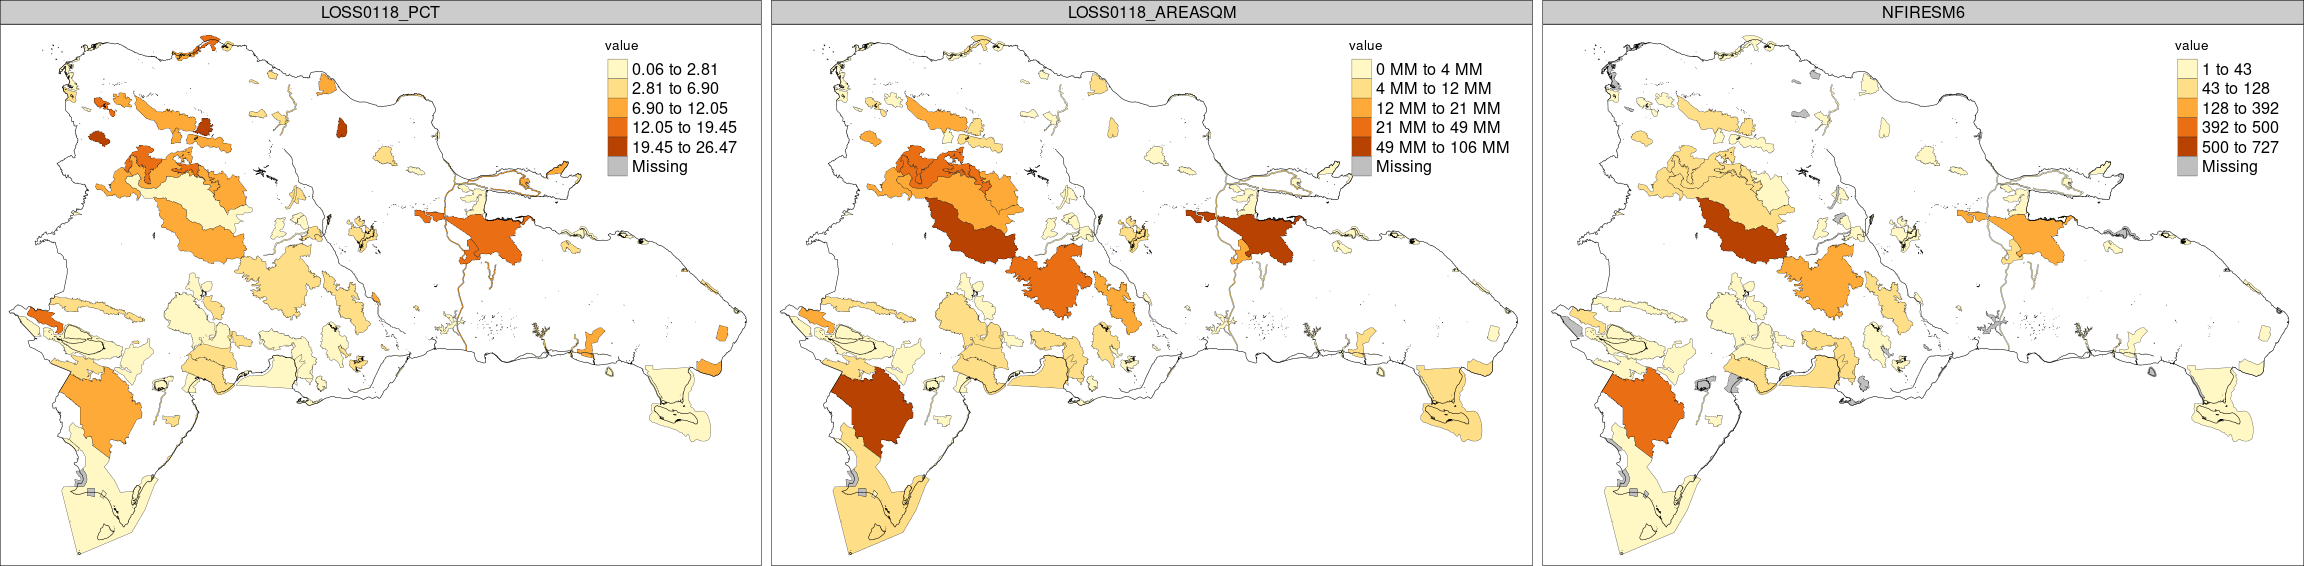
\includegraphics{img/data-download-preparation-eda/zonal-pa-8} \end{center}

\begin{Shaded}
\begin{Highlighting}[]
\CommentTok{\# Top twenty sorted descending by column 2}
\FunctionTok{stripped\_table}\NormalTok{(pazonal }\SpecialCharTok{\%\textgreater{}\%} \FunctionTok{select}\NormalTok{(CATEGORY\_NAME, }\FunctionTok{matches}\NormalTok{(}\StringTok{\textquotesingle{}\^{}LOSS0118|NFIRESM6\textquotesingle{}}\NormalTok{)) }\SpecialCharTok{\%\textgreater{}\%} \FunctionTok{select}\NormalTok{(}\SpecialCharTok{{-}}\FunctionTok{matches}\NormalTok{(}\StringTok{\textquotesingle{}\textless{}NA\textgreater{}\textquotesingle{}}\NormalTok{)))}
\end{Highlighting}
\end{Shaded}

\begin{table}[H]
\centering
\begin{tabular}[t]{llrrr}
\toprule
  & CATEGORY\_NAME & LOSS0118\_PCT & LOSS0118\_AREASQM & NFIRESM6\\
\midrule
\cellcolor{lightgray}{1} & \cellcolor{lightgray}{Reserva Forestal Cerro Chacuey} & \cellcolor{lightgray}{26.466669} & \cellcolor{lightgray}{13734337} & \cellcolor{lightgray}{82}\\
2 & Via Panoramica Entrada de Mao & 22.627826 & 12301958 & 69\\
\cellcolor{lightgray}{3} & \cellcolor{lightgray}{Reserva Cientifica La Salcedoa} & \cellcolor{lightgray}{21.547307} & \cellcolor{lightgray}{8881026} & \cellcolor{lightgray}{27}\\
4 & Monumento Natural Salto de Socoa & 19.446867 & 13282788 & 53\\
\cellcolor{lightgray}{5} & \cellcolor{lightgray}{Monumento Natural Las Caobas} & \cellcolor{lightgray}{17.889496} & \cellcolor{lightgray}{18868449} & \cellcolor{lightgray}{76}\\
\addlinespace
6 & Parque Nacional Los Haitises & 16.796141 & 106098081 & 308\\
\cellcolor{lightgray}{7} & \cellcolor{lightgray}{Parque Nacional La Hispaniola} & \cellcolor{lightgray}{15.833531} & \cellcolor{lightgray}{8680829} & \cellcolor{lightgray}{14}\\
8 & Refugio de Vida Silvestre Río Chacuey & 14.861968 & 5762642 & 38\\
\cellcolor{lightgray}{9} & \cellcolor{lightgray}{Reserva Forestal Alto Mao} & \cellcolor{lightgray}{14.582918} & \cellcolor{lightgray}{30640838} & \cellcolor{lightgray}{104}\\
10 & Parque Nacional José del Carmen Ramírez & 12.051415 & 90356487 & 727\\
\addlinespace
\cellcolor{lightgray}{11} & \cellcolor{lightgray}{Refugio de Vida Silvestre Cañón Río Gurabo} & \cellcolor{lightgray}{11.817495} & \cellcolor{lightgray}{3564134} & \cellcolor{lightgray}{8}\\
12 & Parque Nacional Punta Espada & 11.570795 & 9515568 & 16\\
\cellcolor{lightgray}{13} & \cellcolor{lightgray}{Via Panoramica Autovia Santo Domingo - Samana - Boulevar del Atlantico} & \cellcolor{lightgray}{11.542791} & \cellcolor{lightgray}{11922785} & \cellcolor{lightgray}{18}\\
14 & Parque Nacional Nalga de Maco & 10.828410 & 17958794 & 117\\
\cellcolor{lightgray}{15} & \cellcolor{lightgray}{Parque Nacional Cabo Cabrón} & \cellcolor{lightgray}{10.811425} & \cellcolor{lightgray}{3851405} & \cellcolor{lightgray}{8}\\
\addlinespace
16 & Monumento Natural Hoyo Claro & 10.450862 & 4106759 & 8\\
\cellcolor{lightgray}{17} & \cellcolor{lightgray}{Parque Nacional Manolo Tavarez Justo} & \cellcolor{lightgray}{9.878937} & \cellcolor{lightgray}{34746840} & \cellcolor{lightgray}{128}\\
18 & Parque Nacional Sierra de Bahoruco & 9.108586 & 99490393 & 500\\
\cellcolor{lightgray}{19} & \cellcolor{lightgray}{Reserva Forestal Las Matas} & \cellcolor{lightgray}{8.968713} & \cellcolor{lightgray}{4285024} & \cellcolor{lightgray}{15}\\
20 & Monumento Natural Río Cumayasa y Cueva de las Maravillas & 8.462986 & 7511724 & 15\\
\bottomrule
\end{tabular}
\end{table}

\begin{Shaded}
\begin{Highlighting}[]

\CommentTok{\# Fires M6. Only AREASQM and FIRESM6}
\NormalTok{pazonal }\SpecialCharTok{\%\textgreater{}\%} \FunctionTok{select}\NormalTok{(}\FunctionTok{matches}\NormalTok{(}\StringTok{\textquotesingle{}\^{}LOSS0118\_AREASQM|NFIRESM6|\^{}NAME\textquotesingle{}}\NormalTok{)) }\SpecialCharTok{\%\textgreater{}\%} \FunctionTok{select}\NormalTok{(}\SpecialCharTok{{-}}\FunctionTok{matches}\NormalTok{(}\StringTok{\textquotesingle{}\textless{}NA\textgreater{}\textquotesingle{}}\NormalTok{)) }\SpecialCharTok{\%\textgreater{}\%} 
  \FunctionTok{gather}\NormalTok{(variable, value, }\SpecialCharTok{{-}}\NormalTok{geom, }\SpecialCharTok{{-}}\NormalTok{NAME) }\SpecialCharTok{\%\textgreater{}\%}
  \FunctionTok{mutate}\NormalTok{(}\AttributeTok{NAME =} \FunctionTok{gsub}\NormalTok{(}\StringTok{"(.\{10,\}?)}\SpecialCharTok{\textbackslash{}\textbackslash{}}\StringTok{s"}\NormalTok{, }\StringTok{"}\SpecialCharTok{\textbackslash{}\textbackslash{}}\StringTok{1}\SpecialCharTok{\textbackslash{}n}\StringTok{"}\NormalTok{, NAME)) }\SpecialCharTok{\%\textgreater{}\%} 
  \CommentTok{\# mutate(NAME=gsub(\textquotesingle{} \textquotesingle{}, \textquotesingle{}\textbackslash{}n\textquotesingle{}, NAME)) \%\textgreater{}\% }
  \FunctionTok{mutate}\NormalTok{(}\AttributeTok{variable =} \FunctionTok{factor}\NormalTok{(variable, }\AttributeTok{levels =} \FunctionTok{unique}\NormalTok{(variable))) }\SpecialCharTok{\%\textgreater{}\%} 
  \FunctionTok{tm\_shape}\NormalTok{() }\SpecialCharTok{+}
  \FunctionTok{tm\_fill}\NormalTok{(}\AttributeTok{col=}\StringTok{\textquotesingle{}value\textquotesingle{}}\NormalTok{, }\AttributeTok{palette =} \StringTok{"YlOrBr"}\NormalTok{, }\AttributeTok{size =} \FloatTok{0.1}\NormalTok{, }\AttributeTok{style =} \StringTok{\textquotesingle{}jenks\textquotesingle{}}\NormalTok{) }\SpecialCharTok{+}
  \FunctionTok{tm\_borders}\NormalTok{(}\AttributeTok{col =} \StringTok{\textquotesingle{}grey15\textquotesingle{}}\NormalTok{, }\AttributeTok{lwd =} \FloatTok{0.3}\NormalTok{) }\SpecialCharTok{+}
  \FunctionTok{tm\_facets}\NormalTok{(}\AttributeTok{by =} \StringTok{"variable"}\NormalTok{, }\AttributeTok{ncol =} \DecValTok{2}\NormalTok{, }\AttributeTok{nrow =} \DecValTok{1}\NormalTok{, }\AttributeTok{free.coords =} \ConstantTok{FALSE}\NormalTok{, }\AttributeTok{free.scales =} \ConstantTok{TRUE}\NormalTok{) }\SpecialCharTok{+}
  \FunctionTok{tm\_layout}\NormalTok{(}\AttributeTok{panel.label.size =} \DecValTok{1}\NormalTok{, }\AttributeTok{legend.title.size =} \DecValTok{1}\NormalTok{, }\AttributeTok{legend.text.size =} \DecValTok{1}\NormalTok{) }\SpecialCharTok{+}
  \FunctionTok{tm\_text}\NormalTok{(}\AttributeTok{text =} \StringTok{\textquotesingle{}NAME\textquotesingle{}}\NormalTok{, }\AttributeTok{size =} \FloatTok{0.5}\NormalTok{, }\AttributeTok{auto.placement =}\NormalTok{ T, }\AttributeTok{col =} \StringTok{\textquotesingle{}black\textquotesingle{}}\NormalTok{) }\SpecialCharTok{+} 
  \FunctionTok{tm\_shape}\NormalTok{(}\AttributeTok{shp =}\NormalTok{ cline) }\SpecialCharTok{+} \FunctionTok{tm\_borders}\NormalTok{(}\AttributeTok{col =} \StringTok{\textquotesingle{}black\textquotesingle{}}\NormalTok{, }\AttributeTok{lwd =} \FloatTok{0.5}\NormalTok{)}
\end{Highlighting}
\end{Shaded}

\begin{center}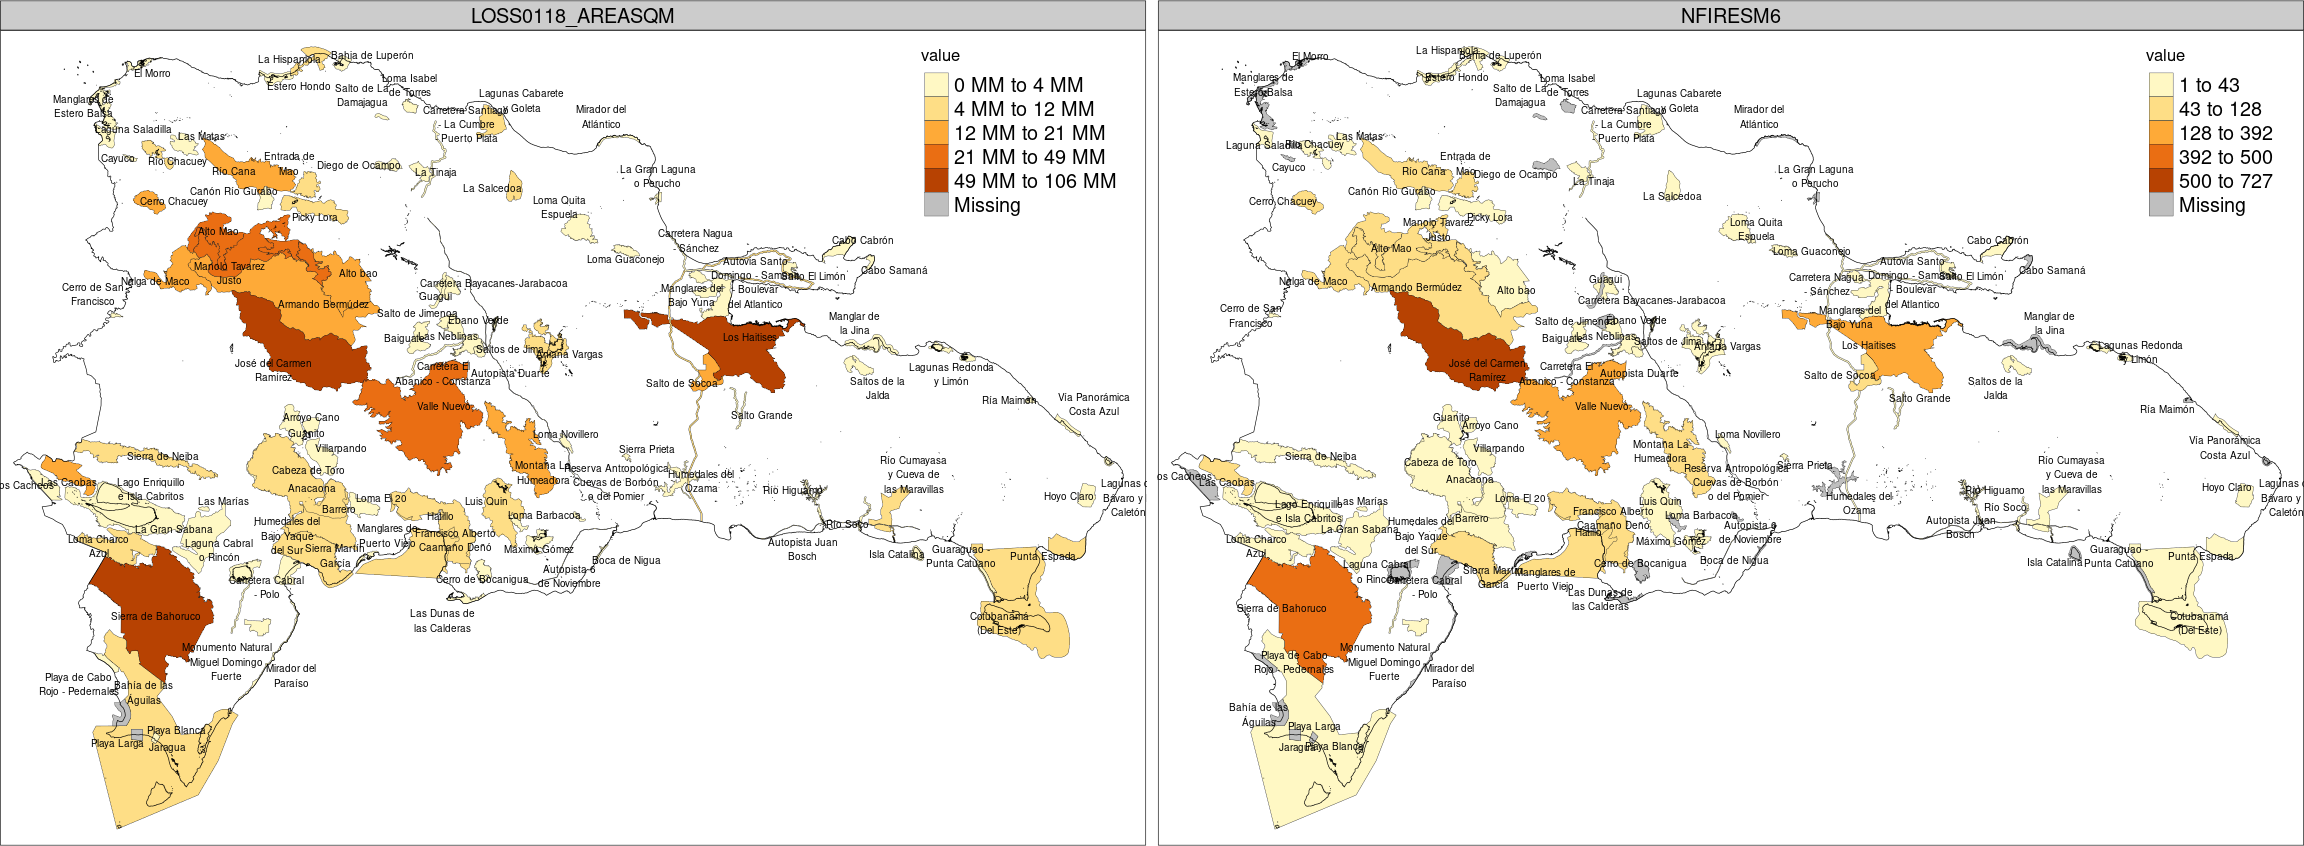
\includegraphics{img/data-download-preparation-eda/zonal-pa-9} \end{center}

\begin{Shaded}
\begin{Highlighting}[]
\CommentTok{\# Top twenty sorted descending by column 2}
\FunctionTok{stripped\_table}\NormalTok{(}
\NormalTok{  pazonal }\SpecialCharTok{\%\textgreater{}\%} \FunctionTok{select}\NormalTok{(CATEGORY\_NAME, }\FunctionTok{matches}\NormalTok{(}\StringTok{\textquotesingle{}\^{}LOSS0118\_AREASQM|NFIRESM6\textquotesingle{}}\NormalTok{)) }\SpecialCharTok{\%\textgreater{}\%}
    \FunctionTok{select}\NormalTok{(}\SpecialCharTok{{-}}\FunctionTok{matches}\NormalTok{(}\StringTok{\textquotesingle{}\textless{}NA\textgreater{}\textquotesingle{}}\NormalTok{))}
\NormalTok{)}
\end{Highlighting}
\end{Shaded}

\begin{table}[H]
\centering
\begin{tabular}[t]{llrr}
\toprule
  & CATEGORY\_NAME & LOSS0118\_AREASQM & NFIRESM6\\
\midrule
\cellcolor{lightgray}{1} & \cellcolor{lightgray}{Parque Nacional Los Haitises} & \cellcolor{lightgray}{106098081} & \cellcolor{lightgray}{308}\\
2 & Parque Nacional Sierra de Bahoruco & 99490393 & 500\\
\cellcolor{lightgray}{3} & \cellcolor{lightgray}{Parque Nacional José del Carmen Ramírez} & \cellcolor{lightgray}{90356487} & \cellcolor{lightgray}{727}\\
4 & Parque Nacional Valle Nuevo & 48606234 & 392\\
\cellcolor{lightgray}{5} & \cellcolor{lightgray}{Parque Nacional Manolo Tavarez Justo} & \cellcolor{lightgray}{34746840} & \cellcolor{lightgray}{128}\\
\addlinespace
6 & Reserva Forestal Alto Mao & 30640838 & 104\\
\cellcolor{lightgray}{7} & \cellcolor{lightgray}{Reserva Forestal Alto bao} & \cellcolor{lightgray}{21401203} & \cellcolor{lightgray}{23}\\
8 & Reserva Forestal Río Cana & 19467164 & 53\\
\cellcolor{lightgray}{9} & \cellcolor{lightgray}{Monumento Natural Las Caobas} & \cellcolor{lightgray}{18868449} & \cellcolor{lightgray}{76}\\
10 & Parque Nacional Montaña La Humeadora & 18277567 & 82\\
\addlinespace
\cellcolor{lightgray}{11} & \cellcolor{lightgray}{Parque Nacional Nalga de Maco} & \cellcolor{lightgray}{17958794} & \cellcolor{lightgray}{117}\\
12 & Parque Nacional Armando Bermúdez & 17271703 & 79\\
\cellcolor{lightgray}{13} & \cellcolor{lightgray}{Reserva Forestal Cerro Chacuey} & \cellcolor{lightgray}{13734337} & \cellcolor{lightgray}{82}\\
14 & Monumento Natural Salto de Socoa & 13282788 & 53\\
\cellcolor{lightgray}{15} & \cellcolor{lightgray}{Via Panoramica Entrada de Mao} & \cellcolor{lightgray}{12301958} & \cellcolor{lightgray}{69}\\
\addlinespace
16 & Via Panoramica Autovia Santo Domingo - Samana - Boulevar del Atlantico & 11922785 & 18\\
\cellcolor{lightgray}{17} & \cellcolor{lightgray}{Reserva Forestal Barrero} & \cellcolor{lightgray}{10128739} & \cellcolor{lightgray}{20}\\
18 & Parque Nacional Punta Espada & 9515568 & 16\\
\cellcolor{lightgray}{19} & \cellcolor{lightgray}{Reserva Biológica Loma Charco Azul} & \cellcolor{lightgray}{9334805} & \cellcolor{lightgray}{22}\\
20 & Reserva Cientifica La Salcedoa & 8881026 & 27\\
\bottomrule
\end{tabular}
\end{table}

\begin{Shaded}
\begin{Highlighting}[]
\CommentTok{\# Top twenty sorted descending by column 2}
\FunctionTok{stripped\_table}\NormalTok{(}
\NormalTok{  pazonal }\SpecialCharTok{\%\textgreater{}\%}
    \FunctionTok{select}\NormalTok{(CATEGORY\_NAME, }\FunctionTok{matches}\NormalTok{(}\StringTok{\textquotesingle{}\^{}LOSS0118\_AREASQM|NFIRESM6\textquotesingle{}}\NormalTok{)) }\SpecialCharTok{\%\textgreater{}\%}
    \FunctionTok{select}\NormalTok{(}\SpecialCharTok{{-}}\FunctionTok{matches}\NormalTok{(}\StringTok{\textquotesingle{}\textless{}NA\textgreater{}\textquotesingle{}}\NormalTok{)),}
  \AttributeTok{order\_col =} \DecValTok{3}
\NormalTok{)}
\end{Highlighting}
\end{Shaded}

\begin{table}[H]
\centering
\begin{tabular}[t]{llrr}
\toprule
  & CATEGORY\_NAME & LOSS0118\_AREASQM & NFIRESM6\\
\midrule
\cellcolor{lightgray}{1} & \cellcolor{lightgray}{Parque Nacional José del Carmen Ramírez} & \cellcolor{lightgray}{90356487} & \cellcolor{lightgray}{727}\\
2 & Parque Nacional Sierra de Bahoruco & 99490393 & 500\\
\cellcolor{lightgray}{3} & \cellcolor{lightgray}{Parque Nacional Valle Nuevo} & \cellcolor{lightgray}{48606234} & \cellcolor{lightgray}{392}\\
4 & Parque Nacional Los Haitises & 106098081 & 308\\
\cellcolor{lightgray}{5} & \cellcolor{lightgray}{Parque Nacional Manolo Tavarez Justo} & \cellcolor{lightgray}{34746840} & \cellcolor{lightgray}{128}\\
\addlinespace
6 & Parque Nacional Nalga de Maco & 17958794 & 117\\
\cellcolor{lightgray}{7} & \cellcolor{lightgray}{Reserva Forestal Alto Mao} & \cellcolor{lightgray}{30640838} & \cellcolor{lightgray}{104}\\
8 & Reserva Forestal Cerro Chacuey & 13734337 & 82\\
\cellcolor{lightgray}{9} & \cellcolor{lightgray}{Parque Nacional Montaña La Humeadora} & \cellcolor{lightgray}{18277567} & \cellcolor{lightgray}{82}\\
10 & Parque Nacional Francisco Alberto Caamaño Deñó & 6035530 & 81\\
\addlinespace
\cellcolor{lightgray}{11} & \cellcolor{lightgray}{Parque Nacional Armando Bermúdez} & \cellcolor{lightgray}{17271703} & \cellcolor{lightgray}{79}\\
12 & Reserva Forestal Hatillo & 6270945 & 76\\
\cellcolor{lightgray}{13} & \cellcolor{lightgray}{Monumento Natural Las Caobas} & \cellcolor{lightgray}{18868449} & \cellcolor{lightgray}{76}\\
14 & Parque Nacional Sierra Martín García & 8441457 & 76\\
\cellcolor{lightgray}{15} & \cellcolor{lightgray}{Via Panoramica Entrada de Mao} & \cellcolor{lightgray}{12301958} & \cellcolor{lightgray}{69}\\
\addlinespace
16 & Reserva Forestal Río Cana & 19467164 & 53\\
\cellcolor{lightgray}{17} & \cellcolor{lightgray}{Monumento Natural Salto de Socoa} & \cellcolor{lightgray}{13282788} & \cellcolor{lightgray}{53}\\
18 & Parque Nacional Sierra de Neiba & 7072866 & 43\\
\cellcolor{lightgray}{19} & \cellcolor{lightgray}{Refugio de Vida Silvestre Río Chacuey} & \cellcolor{lightgray}{5762642} & \cellcolor{lightgray}{38}\\
20 & Reserva Forestal Villarpando & 3377307 & 34\\
\bottomrule
\end{tabular}
\end{table}

\begin{Shaded}
\begin{Highlighting}[]

\CommentTok{\# Fires V1}
\NormalTok{pazonal }\SpecialCharTok{\%\textgreater{}\%} \FunctionTok{select}\NormalTok{(}\FunctionTok{matches}\NormalTok{(}\StringTok{\textquotesingle{}\^{}LOSS1218|NFIRESV1\textquotesingle{}}\NormalTok{)) }\SpecialCharTok{\%\textgreater{}\%} \FunctionTok{select}\NormalTok{(}\SpecialCharTok{{-}}\FunctionTok{matches}\NormalTok{(}\StringTok{\textquotesingle{}\textless{}NA\textgreater{}\textquotesingle{}}\NormalTok{)) }\SpecialCharTok{\%\textgreater{}\%} 
  \FunctionTok{gather}\NormalTok{(variable, value, }\SpecialCharTok{{-}}\NormalTok{geom) }\SpecialCharTok{\%\textgreater{}\%}
  \FunctionTok{mutate}\NormalTok{(}\AttributeTok{variable =} \FunctionTok{factor}\NormalTok{(variable, }\AttributeTok{levels =} \FunctionTok{unique}\NormalTok{(variable))) }\SpecialCharTok{\%\textgreater{}\%} 
  \FunctionTok{tm\_shape}\NormalTok{() }\SpecialCharTok{+}
  \FunctionTok{tm\_fill}\NormalTok{(}\AttributeTok{col=}\StringTok{\textquotesingle{}value\textquotesingle{}}\NormalTok{, }\AttributeTok{palette =} \StringTok{"YlOrBr"}\NormalTok{, }\AttributeTok{size =} \FloatTok{0.1}\NormalTok{, }\AttributeTok{style =} \StringTok{\textquotesingle{}jenks\textquotesingle{}}\NormalTok{) }\SpecialCharTok{+}
  \FunctionTok{tm\_borders}\NormalTok{(}\AttributeTok{col =} \StringTok{\textquotesingle{}grey15\textquotesingle{}}\NormalTok{, }\AttributeTok{lwd =} \FloatTok{0.3}\NormalTok{) }\SpecialCharTok{+}
  \FunctionTok{tm\_facets}\NormalTok{(}\AttributeTok{by =} \StringTok{"variable"}\NormalTok{, }\AttributeTok{ncol =} \DecValTok{3}\NormalTok{, }\AttributeTok{nrow =} \DecValTok{1}\NormalTok{, }\AttributeTok{free.coords =} \ConstantTok{FALSE}\NormalTok{, }\AttributeTok{free.scales =} \ConstantTok{TRUE}\NormalTok{) }\SpecialCharTok{+}
  \FunctionTok{tm\_layout}\NormalTok{(}\AttributeTok{panel.label.size =} \DecValTok{1}\NormalTok{, }\AttributeTok{legend.title.size =} \DecValTok{1}\NormalTok{, }\AttributeTok{legend.text.size =} \DecValTok{1}\NormalTok{) }\SpecialCharTok{+} 
  \FunctionTok{tm\_shape}\NormalTok{(}\AttributeTok{shp =}\NormalTok{ cline) }\SpecialCharTok{+} \FunctionTok{tm\_borders}\NormalTok{(}\AttributeTok{col =} \StringTok{\textquotesingle{}black\textquotesingle{}}\NormalTok{, }\AttributeTok{lwd =} \FloatTok{0.5}\NormalTok{)}
\end{Highlighting}
\end{Shaded}

\begin{center}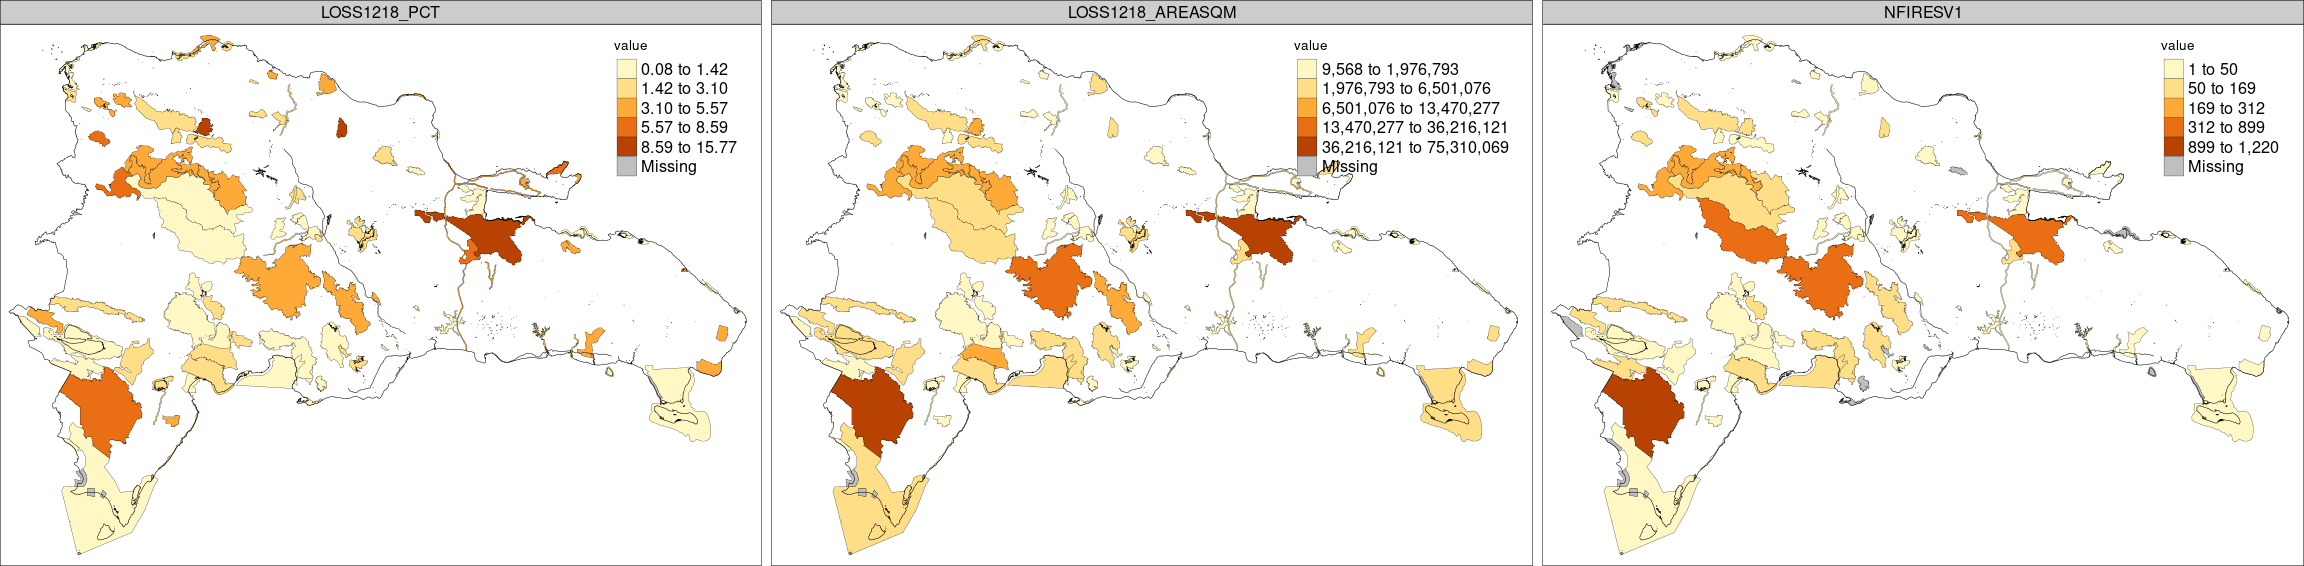
\includegraphics{img/data-download-preparation-eda/zonal-pa-10} \end{center}

\begin{Shaded}
\begin{Highlighting}[]
\CommentTok{\# Top twenty sorted descending by column 2}
\FunctionTok{stripped\_table}\NormalTok{(pazonal }\SpecialCharTok{\%\textgreater{}\%} \FunctionTok{select}\NormalTok{(CATEGORY\_NAME, }\FunctionTok{matches}\NormalTok{(}\StringTok{\textquotesingle{}\^{}LOSS1218|NFIRESV1\textquotesingle{}}\NormalTok{)) }\SpecialCharTok{\%\textgreater{}\%} \FunctionTok{select}\NormalTok{(}\SpecialCharTok{{-}}\FunctionTok{matches}\NormalTok{(}\StringTok{\textquotesingle{}\textless{}NA\textgreater{}\textquotesingle{}}\NormalTok{)))}
\end{Highlighting}
\end{Shaded}

\begin{table}[H]
\centering
\begin{tabular}[t]{llrrr}
\toprule
  & CATEGORY\_NAME & LOSS1218\_PCT & LOSS1218\_AREASQM & NFIRESV1\\
\midrule
\cellcolor{lightgray}{1} & \cellcolor{lightgray}{Reserva Cientifica La Salcedoa} & \cellcolor{lightgray}{15.773028} & \cellcolor{lightgray}{6501076.2} & \cellcolor{lightgray}{66}\\
2 & Via Panoramica Entrada de Mao & 14.178246 & 7708217.1 & 132\\
\cellcolor{lightgray}{3} & \cellcolor{lightgray}{Parque Nacional Los Haitises} & \cellcolor{lightgray}{11.668154} & \cellcolor{lightgray}{73705545.1} & \cellcolor{lightgray}{694}\\
4 & Reserva Forestal Cerro Chacuey & 8.593019 & 4459171.5 & 106\\
\cellcolor{lightgray}{5} & \cellcolor{lightgray}{Monumento Natural Salto de Socoa} & \cellcolor{lightgray}{8.132287} & \cellcolor{lightgray}{5554593.8} & \cellcolor{lightgray}{92}\\
\addlinespace
6 & Parque Nacional Cabo Cabrón & 7.604139 & 2708858.5 & 16\\
\cellcolor{lightgray}{7} & \cellcolor{lightgray}{Parque Nacional Sierra de Bahoruco} & \cellcolor{lightgray}{6.894819} & \cellcolor{lightgray}{75310069.2} & \cellcolor{lightgray}{1220}\\
8 & Parque Nacional Nalga de Maco & 5.986853 & 9929126.7 & 259\\
\cellcolor{lightgray}{9} & \cellcolor{lightgray}{Monumento Natural Hoyo Claro} & \cellcolor{lightgray}{5.567929} & \cellcolor{lightgray}{2187967.0} & \cellcolor{lightgray}{27}\\
10 & Monumento Natural Las Caobas & 5.444326 & 5742251.6 & 85\\
\addlinespace
\cellcolor{lightgray}{11} & \cellcolor{lightgray}{Monumento Natural Salto El Limón} & \cellcolor{lightgray}{5.137017} & \cellcolor{lightgray}{846322.8} & \cellcolor{lightgray}{16}\\
12 & Reserva Forestal Alto Mao & 5.100222 & 10716311.3 & 240\\
\cellcolor{lightgray}{13} & \cellcolor{lightgray}{Refugio de Vida Silvestre Río Chacuey} & \cellcolor{lightgray}{5.098188} & \cellcolor{lightgray}{1976792.9} & \cellcolor{lightgray}{67}\\
14 & Monumento Natural Río Cumayasa y Cueva de las Maravillas & 4.811717 & 4270867.5 & 41\\
\cellcolor{lightgray}{15} & \cellcolor{lightgray}{Monumento Natural Cabo Samaná} & \cellcolor{lightgray}{4.624415} & \cellcolor{lightgray}{428710.5} & \cellcolor{lightgray}{8}\\
\addlinespace
16 & Parque Nacional Punta Espada & 4.278458 & 3518509.8 & 30\\
\cellcolor{lightgray}{17} & \cellcolor{lightgray}{Monumento Natural Loma Isabel de Torres} & \cellcolor{lightgray}{4.185139} & \cellcolor{lightgray}{694938.9} & \cellcolor{lightgray}{1}\\
18 & Via Panoramica Mirador del Atlántico & 4.129220 & 500296.5 & NA\\
\cellcolor{lightgray}{19} & \cellcolor{lightgray}{Parque Nacional Saltos de la Jalda} & \cellcolor{lightgray}{4.004362} & \cellcolor{lightgray}{1458936.7} & \cellcolor{lightgray}{2}\\
20 & Parque Nacional Valle Nuevo & 3.996785 & 36216121.2 & 899\\
\bottomrule
\end{tabular}
\end{table}

\hypertarget{zonal-by-grid-used-in-the-long-term-analytical-approach}{%
\subsection{Zonal, by grid used in the long-term analytical
approach}\label{zonal-by-grid-used-in-the-long-term-analytical-approach}}

\begin{Shaded}
\begin{Highlighting}[]
\CommentTok{\#Zonal statistics object}
\NormalTok{grdzonal }\OtherTok{\textless{}{-}} \FunctionTok{readRDS}\NormalTok{(}\StringTok{\textquotesingle{}out/grd\_zonal\_statistics.RDS\textquotesingle{}}\NormalTok{)}

\CommentTok{\# Tree cover for pctc threshold}
\NormalTok{grdzonal }\SpecialCharTok{\%\textgreater{}\%} \FunctionTok{select}\NormalTok{(}\FunctionTok{matches}\NormalTok{(}\StringTok{\textquotesingle{}\^{}TREECOVER2000\textquotesingle{}}\NormalTok{)) }\SpecialCharTok{\%\textgreater{}\%}
  \FunctionTok{gather}\NormalTok{(variable, value, }\SpecialCharTok{{-}}\NormalTok{geometry) }\SpecialCharTok{\%\textgreater{}\%}
  \FunctionTok{tm\_shape}\NormalTok{() }\SpecialCharTok{+}
  \FunctionTok{tm\_fill}\NormalTok{(}\AttributeTok{col=}\StringTok{\textquotesingle{}value\textquotesingle{}}\NormalTok{, }\AttributeTok{palette =} \StringTok{"YlOrBr"}\NormalTok{, }\AttributeTok{size =} \FloatTok{0.1}\NormalTok{, }\AttributeTok{style =} \StringTok{\textquotesingle{}kmeans\textquotesingle{}}\NormalTok{) }\SpecialCharTok{+}
  \FunctionTok{tm\_borders}\NormalTok{(}\AttributeTok{col =} \StringTok{\textquotesingle{}grey15\textquotesingle{}}\NormalTok{, }\AttributeTok{lwd =} \FloatTok{0.3}\NormalTok{) }\SpecialCharTok{+}
  \FunctionTok{tm\_facets}\NormalTok{(}\AttributeTok{by =} \StringTok{"variable"}\NormalTok{, }\AttributeTok{ncol =} \DecValTok{2}\NormalTok{, }\AttributeTok{nrow =} \DecValTok{2}\NormalTok{, }\AttributeTok{free.coords =} \ConstantTok{FALSE}\NormalTok{, }\AttributeTok{free.scales =} \ConstantTok{TRUE}\NormalTok{) }\SpecialCharTok{+}
  \FunctionTok{tm\_layout}\NormalTok{(}\AttributeTok{panel.label.size =} \DecValTok{2}\NormalTok{, }\AttributeTok{legend.title.size =} \DecValTok{2}\NormalTok{, }\AttributeTok{legend.text.size =} \FloatTok{1.5}\NormalTok{) }\SpecialCharTok{+}
  \FunctionTok{tm\_shape}\NormalTok{(prov) }\SpecialCharTok{+} \FunctionTok{tm\_borders}\NormalTok{()}
\end{Highlighting}
\end{Shaded}

\begin{center}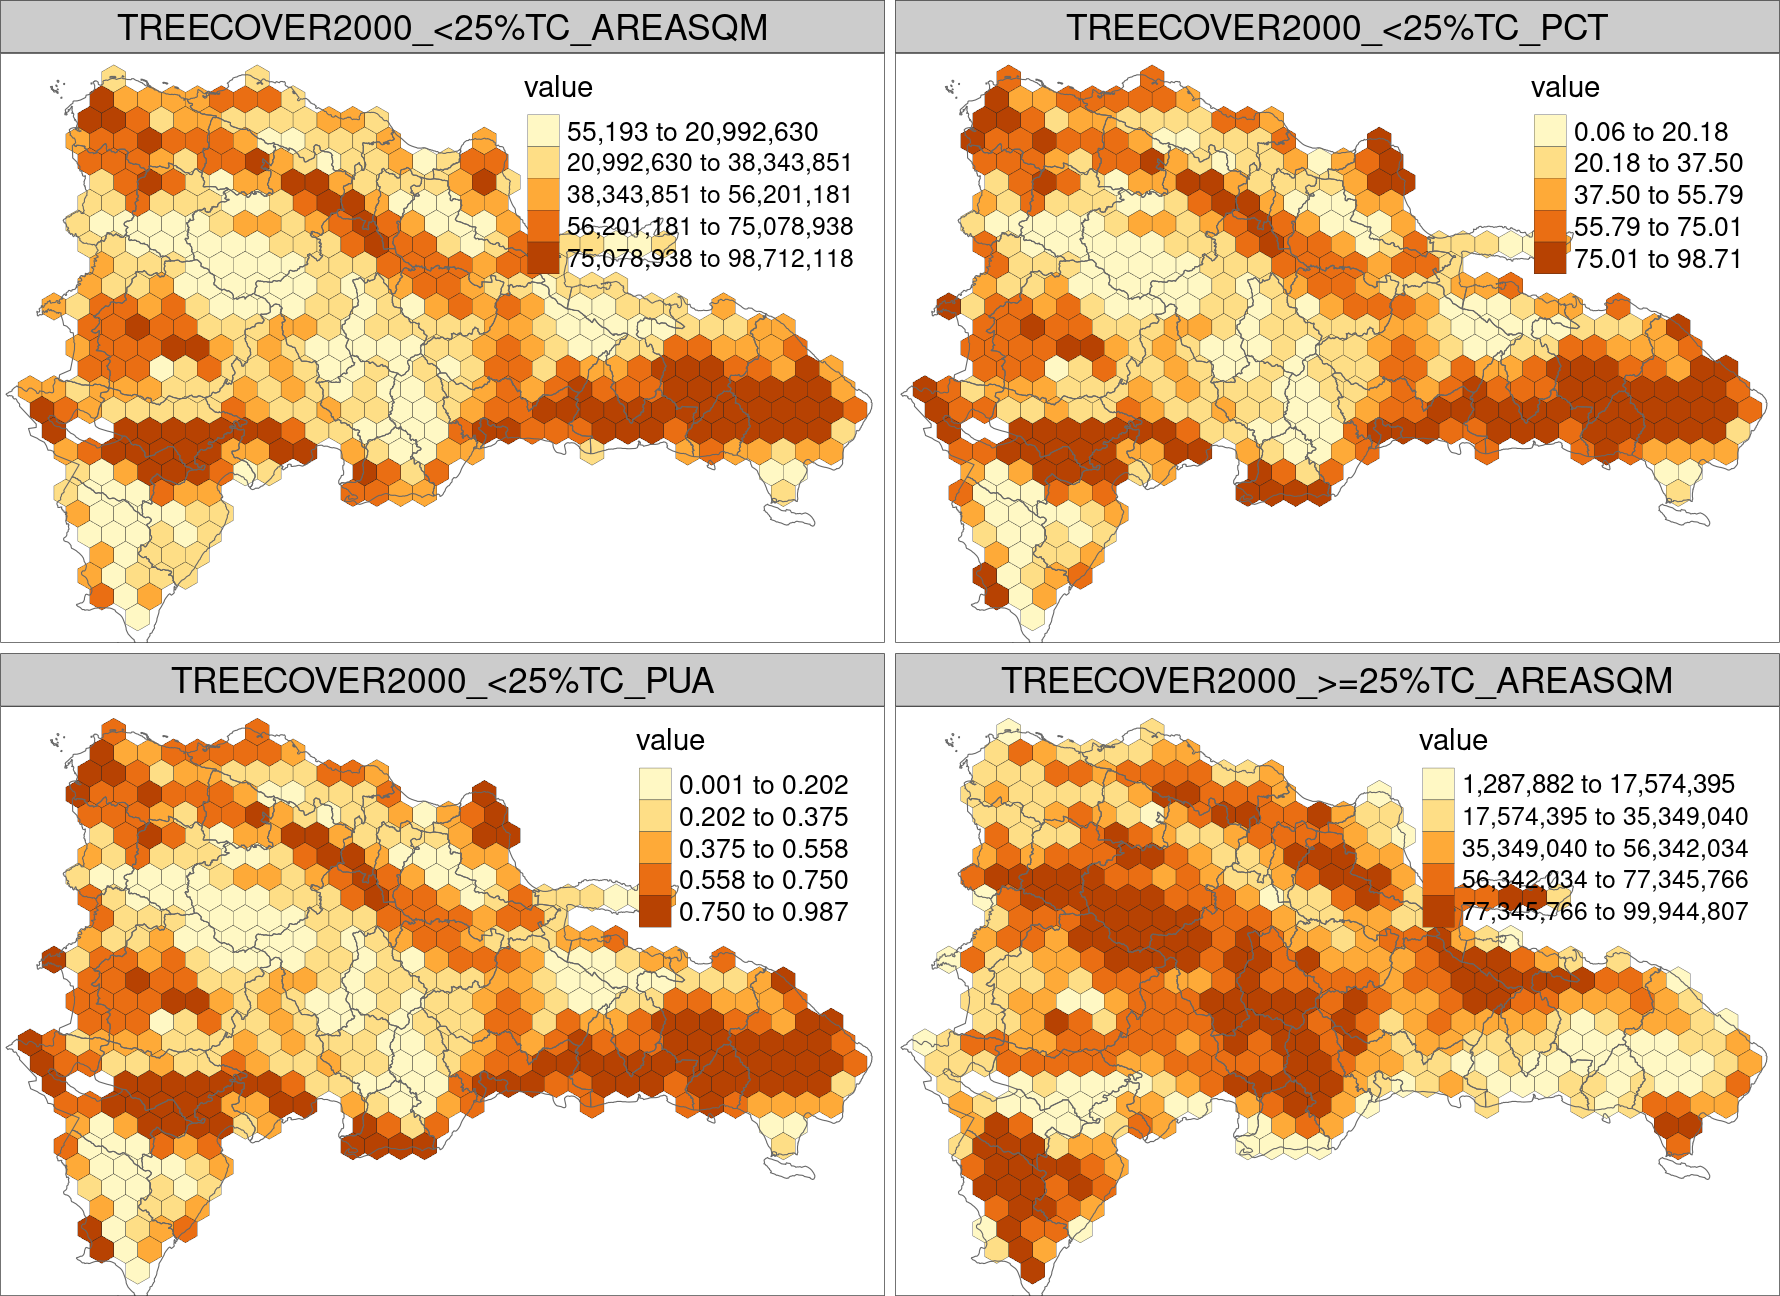
\includegraphics{img/data-download-preparation-eda/zonal-long-term-grid-1} \end{center}

\begin{verbatim}
## ================================================================================
\end{verbatim}

\begin{center}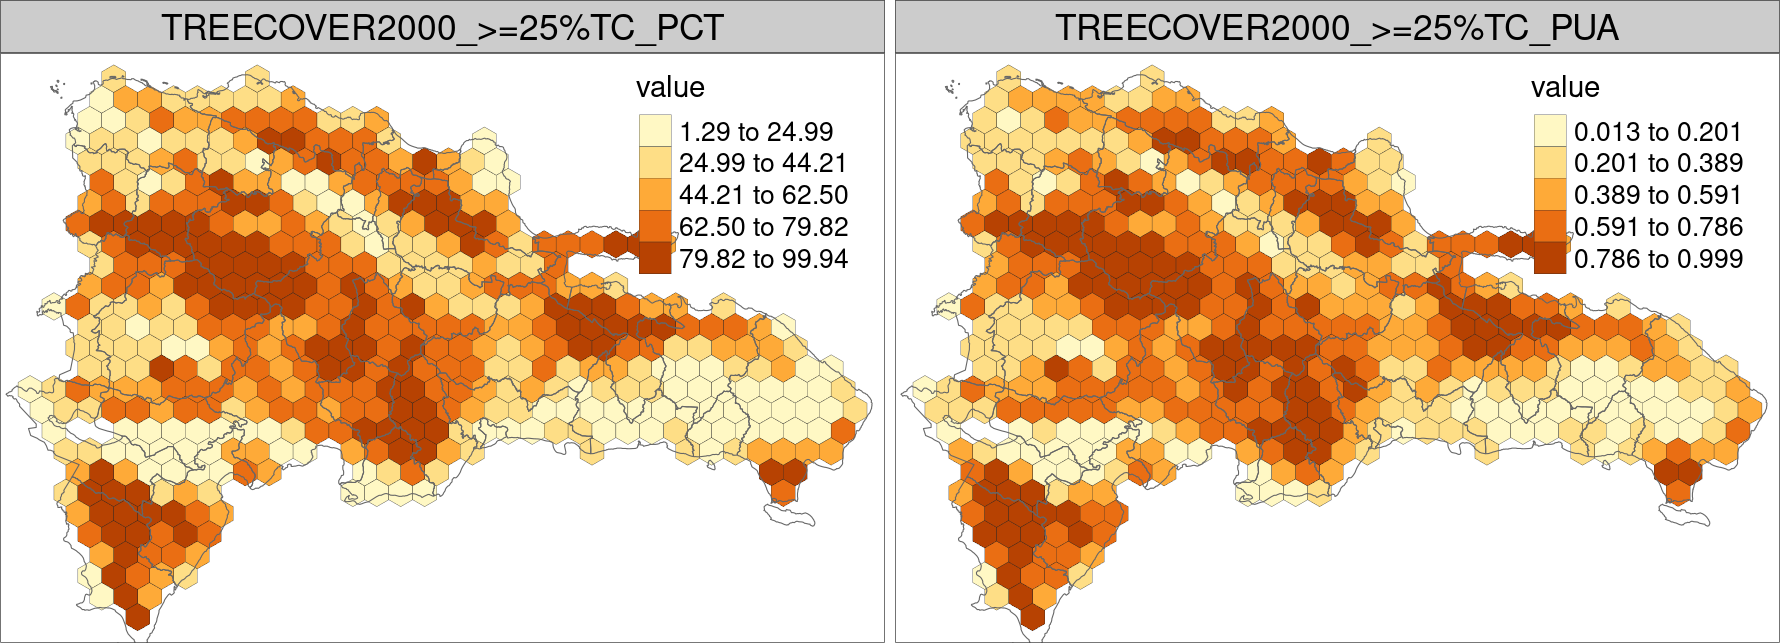
\includegraphics{img/data-download-preparation-eda/zonal-long-term-grid-2} \end{center}

\begin{Shaded}
\begin{Highlighting}[]

\CommentTok{\# Loss year}
\CommentTok{\# * PCT}
\NormalTok{grdzonal }\SpecialCharTok{\%\textgreater{}\%}\NormalTok{ dplyr}\SpecialCharTok{::}\FunctionTok{select}\NormalTok{(}\FunctionTok{matches}\NormalTok{(}\StringTok{\textquotesingle{}\^{}LOSSYEAR\_[1{-}9].*\_PCT$\textquotesingle{}}\NormalTok{)) }\SpecialCharTok{\%\textgreater{}\%}
  \FunctionTok{gather}\NormalTok{(variable, value, }\SpecialCharTok{{-}}\NormalTok{geometry) }\SpecialCharTok{\%\textgreater{}\%}
  \FunctionTok{mutate}\NormalTok{(}\AttributeTok{variable =} \FunctionTok{factor}\NormalTok{(variable, }\AttributeTok{levels =} \FunctionTok{unique}\NormalTok{(variable))) }\SpecialCharTok{\%\textgreater{}\%} 
  \FunctionTok{tm\_shape}\NormalTok{() }\SpecialCharTok{+}
  \FunctionTok{tm\_fill}\NormalTok{(}\AttributeTok{col=}\StringTok{\textquotesingle{}value\textquotesingle{}}\NormalTok{, }\AttributeTok{palette =} \StringTok{"YlOrBr"}\NormalTok{, }\AttributeTok{size =} \FloatTok{0.1}\NormalTok{, }\AttributeTok{style =} \StringTok{\textquotesingle{}kmeans\textquotesingle{}}\NormalTok{) }\SpecialCharTok{+}
  \FunctionTok{tm\_borders}\NormalTok{(}\AttributeTok{col =} \StringTok{\textquotesingle{}grey15\textquotesingle{}}\NormalTok{, }\AttributeTok{lwd =} \FloatTok{0.3}\NormalTok{) }\SpecialCharTok{+}
  \FunctionTok{tm\_facets}\NormalTok{(}\AttributeTok{by =} \StringTok{"variable"}\NormalTok{, }\AttributeTok{ncol =} \DecValTok{6}\NormalTok{, }\AttributeTok{nrow =} \DecValTok{3}\NormalTok{, }\AttributeTok{free.coords =} \ConstantTok{FALSE}\NormalTok{, }\AttributeTok{free.scales =} \ConstantTok{TRUE}\NormalTok{) }\SpecialCharTok{+}
  \FunctionTok{tm\_layout}\NormalTok{(}\AttributeTok{panel.label.size =} \DecValTok{2}\NormalTok{, }\AttributeTok{legend.title.size =} \DecValTok{1}\NormalTok{, }\AttributeTok{legend.text.size =} \DecValTok{1}\NormalTok{) }\SpecialCharTok{+}
  \FunctionTok{tm\_shape}\NormalTok{(prov) }\SpecialCharTok{+} \FunctionTok{tm\_borders}\NormalTok{()}
\end{Highlighting}
\end{Shaded}

\begin{center}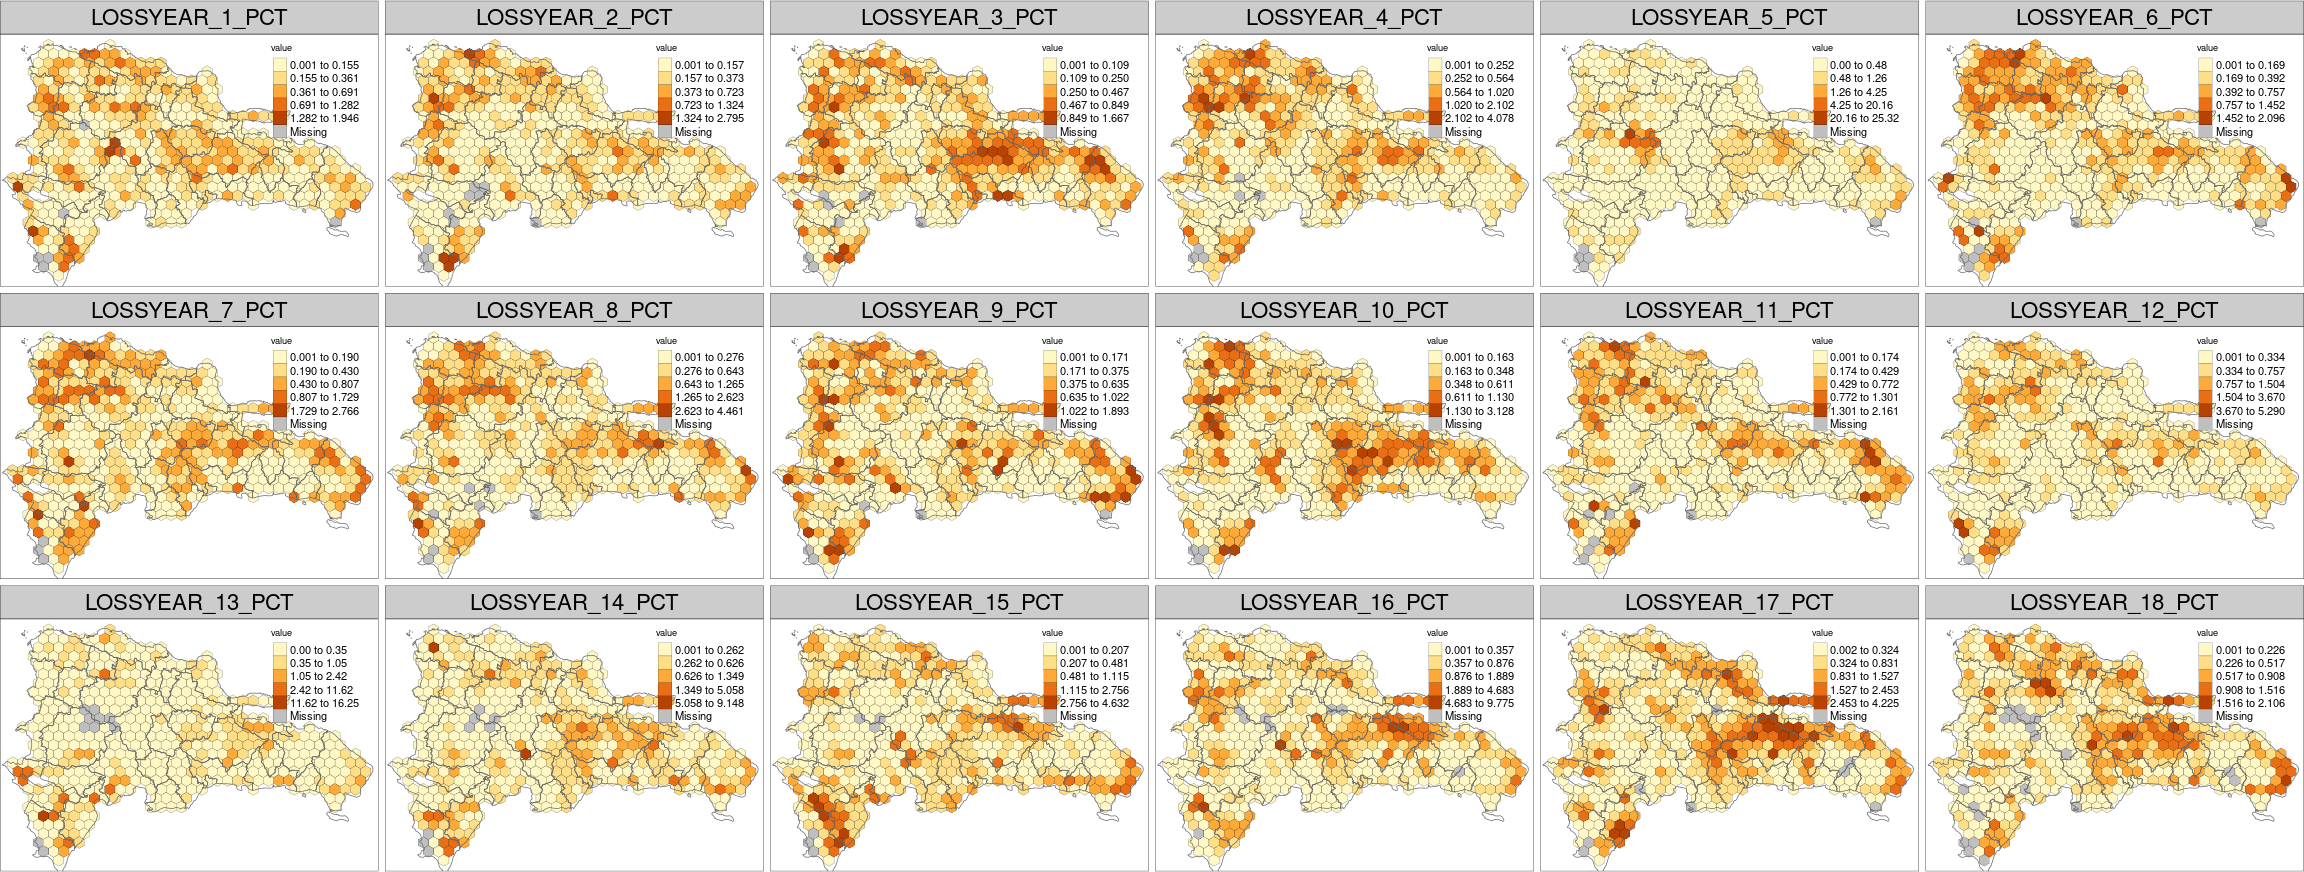
\includegraphics{img/data-download-preparation-eda/zonal-long-term-grid-3} \end{center}

\begin{Shaded}
\begin{Highlighting}[]
\CommentTok{\# * AREASQM}
\NormalTok{grdzonal }\SpecialCharTok{\%\textgreater{}\%}\NormalTok{ dplyr}\SpecialCharTok{::}\FunctionTok{select}\NormalTok{(}\FunctionTok{matches}\NormalTok{(}\StringTok{\textquotesingle{}\^{}LOSSYEAR\_[1{-}9].*AREA.*\textquotesingle{}}\NormalTok{)) }\SpecialCharTok{\%\textgreater{}\%}
  \FunctionTok{gather}\NormalTok{(variable, value, }\SpecialCharTok{{-}}\NormalTok{geometry) }\SpecialCharTok{\%\textgreater{}\%}
  \FunctionTok{mutate}\NormalTok{(}\AttributeTok{variable =} \FunctionTok{factor}\NormalTok{(variable, }\AttributeTok{levels =} \FunctionTok{unique}\NormalTok{(variable))) }\SpecialCharTok{\%\textgreater{}\%} 
  \FunctionTok{tm\_shape}\NormalTok{() }\SpecialCharTok{+}
  \FunctionTok{tm\_fill}\NormalTok{(}\AttributeTok{col=}\StringTok{\textquotesingle{}value\textquotesingle{}}\NormalTok{, }\AttributeTok{palette =} \StringTok{"YlOrBr"}\NormalTok{, }\AttributeTok{size =} \FloatTok{0.1}\NormalTok{, }\AttributeTok{style =} \StringTok{\textquotesingle{}kmeans\textquotesingle{}}\NormalTok{) }\SpecialCharTok{+}
  \FunctionTok{tm\_borders}\NormalTok{(}\AttributeTok{col =} \StringTok{\textquotesingle{}grey15\textquotesingle{}}\NormalTok{, }\AttributeTok{lwd =} \FloatTok{0.3}\NormalTok{) }\SpecialCharTok{+}
  \FunctionTok{tm\_facets}\NormalTok{(}\AttributeTok{by =} \StringTok{"variable"}\NormalTok{, }\AttributeTok{ncol =} \DecValTok{6}\NormalTok{, }\AttributeTok{nrow =} \DecValTok{3}\NormalTok{, }\AttributeTok{free.coords =} \ConstantTok{FALSE}\NormalTok{, }\AttributeTok{free.scales =} \ConstantTok{TRUE}\NormalTok{) }\SpecialCharTok{+}
  \FunctionTok{tm\_layout}\NormalTok{(}\AttributeTok{panel.label.size =} \DecValTok{2}\NormalTok{, }\AttributeTok{legend.title.size =} \DecValTok{1}\NormalTok{, }\AttributeTok{legend.text.size =} \DecValTok{1}\NormalTok{) }\SpecialCharTok{+}
  \FunctionTok{tm\_shape}\NormalTok{(prov) }\SpecialCharTok{+} \FunctionTok{tm\_borders}\NormalTok{()}
\end{Highlighting}
\end{Shaded}

\begin{center}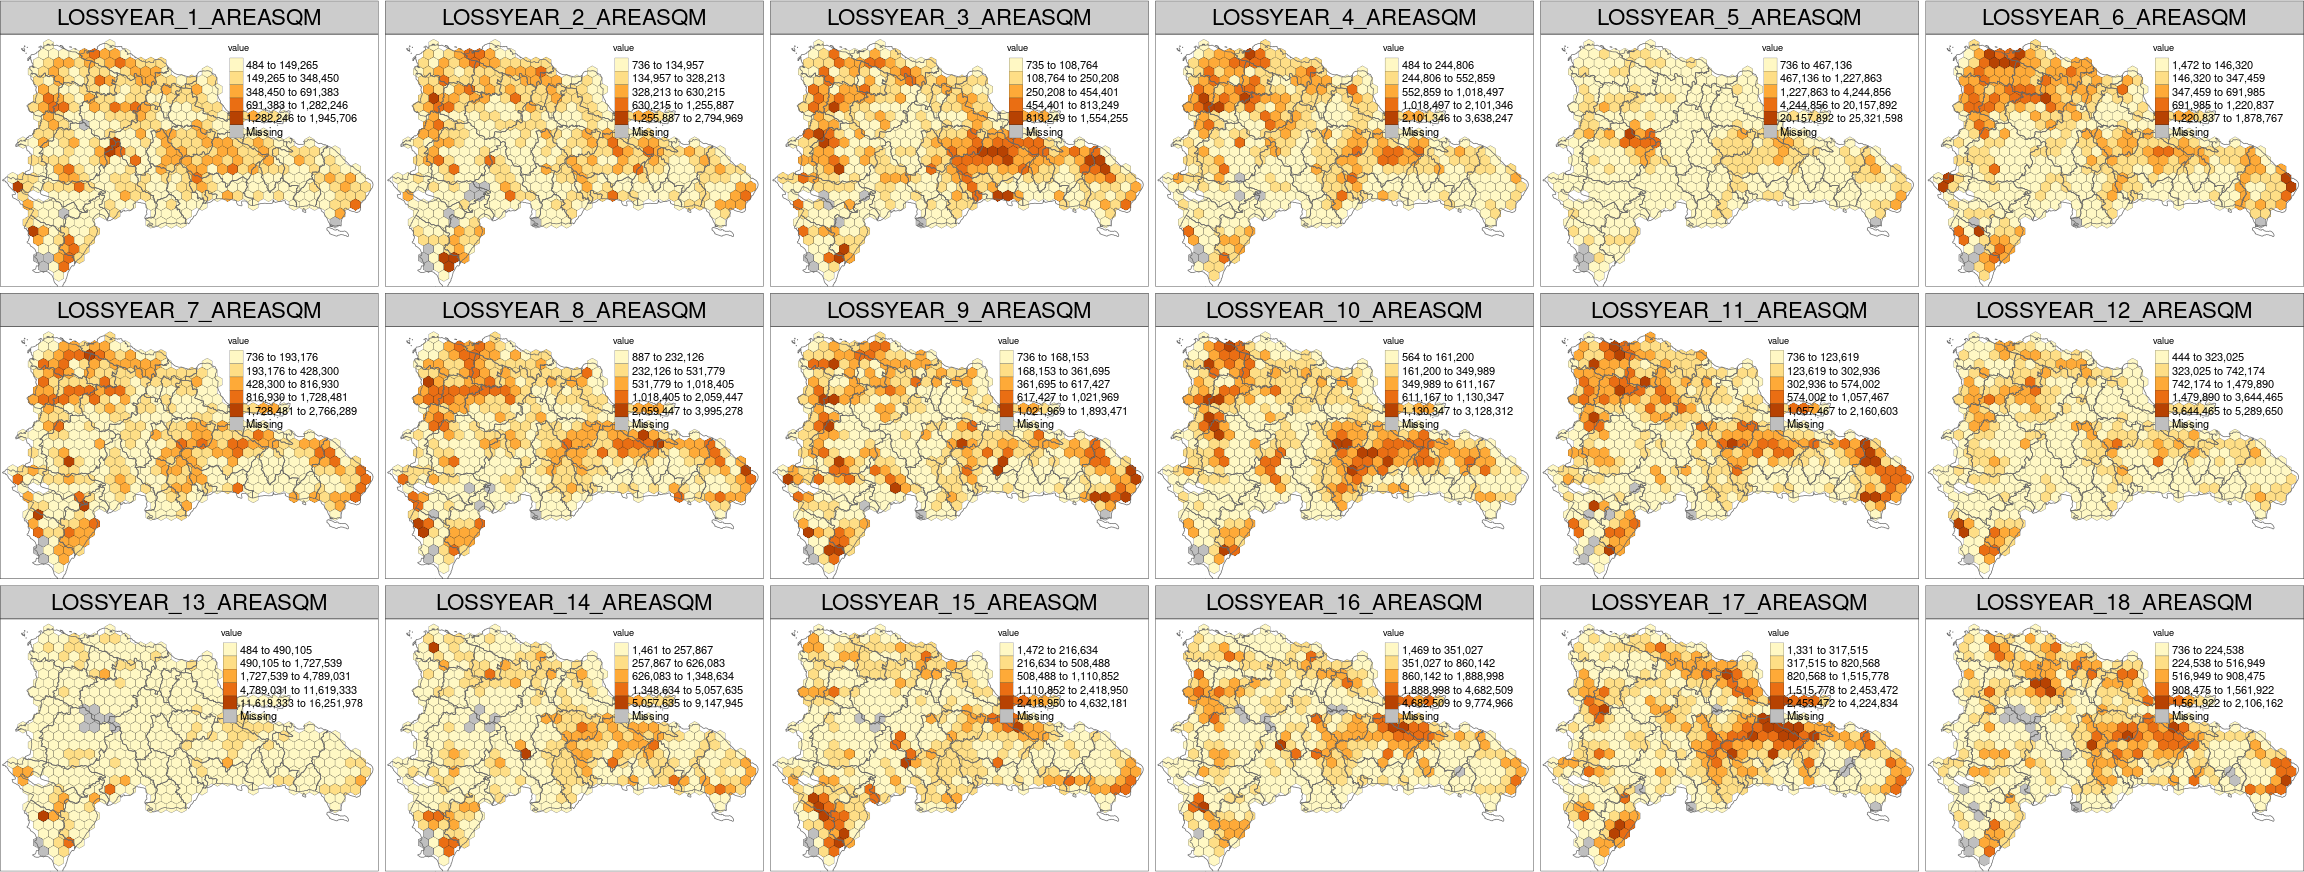
\includegraphics{img/data-download-preparation-eda/zonal-long-term-grid-4} \end{center}

\begin{Shaded}
\begin{Highlighting}[]
\CommentTok{\# * Provinces overlayed, single scale}
\NormalTok{grdzonal }\SpecialCharTok{\%\textgreater{}\%}\NormalTok{ dplyr}\SpecialCharTok{::}\FunctionTok{select}\NormalTok{(}\FunctionTok{matches}\NormalTok{(}\StringTok{\textquotesingle{}\^{}LOSSYEAR\_[1{-}9].*AREA.*\textquotesingle{}}\NormalTok{)) }\SpecialCharTok{\%\textgreater{}\%}
  \FunctionTok{gather}\NormalTok{(variable, value, }\SpecialCharTok{{-}}\NormalTok{geometry) }\SpecialCharTok{\%\textgreater{}\%}
  \FunctionTok{mutate}\NormalTok{(}\AttributeTok{variable =} \FunctionTok{factor}\NormalTok{(variable, }\AttributeTok{levels =} \FunctionTok{unique}\NormalTok{(variable))) }\SpecialCharTok{\%\textgreater{}\%} 
  \FunctionTok{tm\_shape}\NormalTok{() }\SpecialCharTok{+}
  \FunctionTok{tm\_fill}\NormalTok{(}\AttributeTok{col=}\StringTok{\textquotesingle{}value\textquotesingle{}}\NormalTok{, }\AttributeTok{palette =} \StringTok{"YlOrBr"}\NormalTok{, }\AttributeTok{size =} \FloatTok{0.1}\NormalTok{,}
          \AttributeTok{style =} \StringTok{\textquotesingle{}kmeans\textquotesingle{}}\NormalTok{, }\AttributeTok{legend.is.portrait =}\NormalTok{ F, }\AttributeTok{title =} \StringTok{\textquotesingle{}Area (square meters)\textquotesingle{}}\NormalTok{,}
          \AttributeTok{textNA =} \StringTok{"No tree cover loss"}\NormalTok{) }\SpecialCharTok{+}
  \FunctionTok{tm\_borders}\NormalTok{(}\AttributeTok{col =} \StringTok{\textquotesingle{}grey15\textquotesingle{}}\NormalTok{, }\AttributeTok{lwd =} \FloatTok{0.3}\NormalTok{) }\SpecialCharTok{+}
  \FunctionTok{tm\_facets}\NormalTok{(}\AttributeTok{by =} \StringTok{"variable"}\NormalTok{, }\AttributeTok{ncol =} \DecValTok{6}\NormalTok{, }\AttributeTok{nrow =} \DecValTok{3}\NormalTok{, }\AttributeTok{free.coords =} \ConstantTok{FALSE}\NormalTok{, }\AttributeTok{free.scales =} \ConstantTok{FALSE}\NormalTok{) }\SpecialCharTok{+}
  \FunctionTok{tm\_layout}\NormalTok{(}\AttributeTok{panel.label.size =} \DecValTok{3}\NormalTok{, }\AttributeTok{legend.title.size =} \FloatTok{2.5}\NormalTok{, }\AttributeTok{legend.text.size =} \FloatTok{1.5}\NormalTok{,}
            \AttributeTok{legend.outside.position =} \StringTok{"bottom"}\NormalTok{ , }\AttributeTok{legend.outside.size =}\NormalTok{ .}\DecValTok{1}\NormalTok{,}
            \AttributeTok{main.title =} \StringTok{\textquotesingle{}Dominican Republic. Tree cover loss 2001{-}2018\textquotesingle{}}\NormalTok{,}
            \AttributeTok{main.title.size =} \FloatTok{2.5}\NormalTok{, }\AttributeTok{attr.outside=}\ConstantTok{TRUE}\NormalTok{) }\SpecialCharTok{+} 
  \FunctionTok{tm\_credits}\NormalTok{(}\StringTok{\textquotesingle{}Author: José Martínez B.}\SpecialCharTok{\textbackslash{}n}\StringTok{Source: Hansen et al. 2013\textquotesingle{}}\NormalTok{, }\AttributeTok{size =} \DecValTok{2}\NormalTok{) }\SpecialCharTok{+}
  \FunctionTok{tm\_shape}\NormalTok{(prov) }\SpecialCharTok{+} \FunctionTok{tm\_borders}\NormalTok{()}
\end{Highlighting}
\end{Shaded}

\begin{center}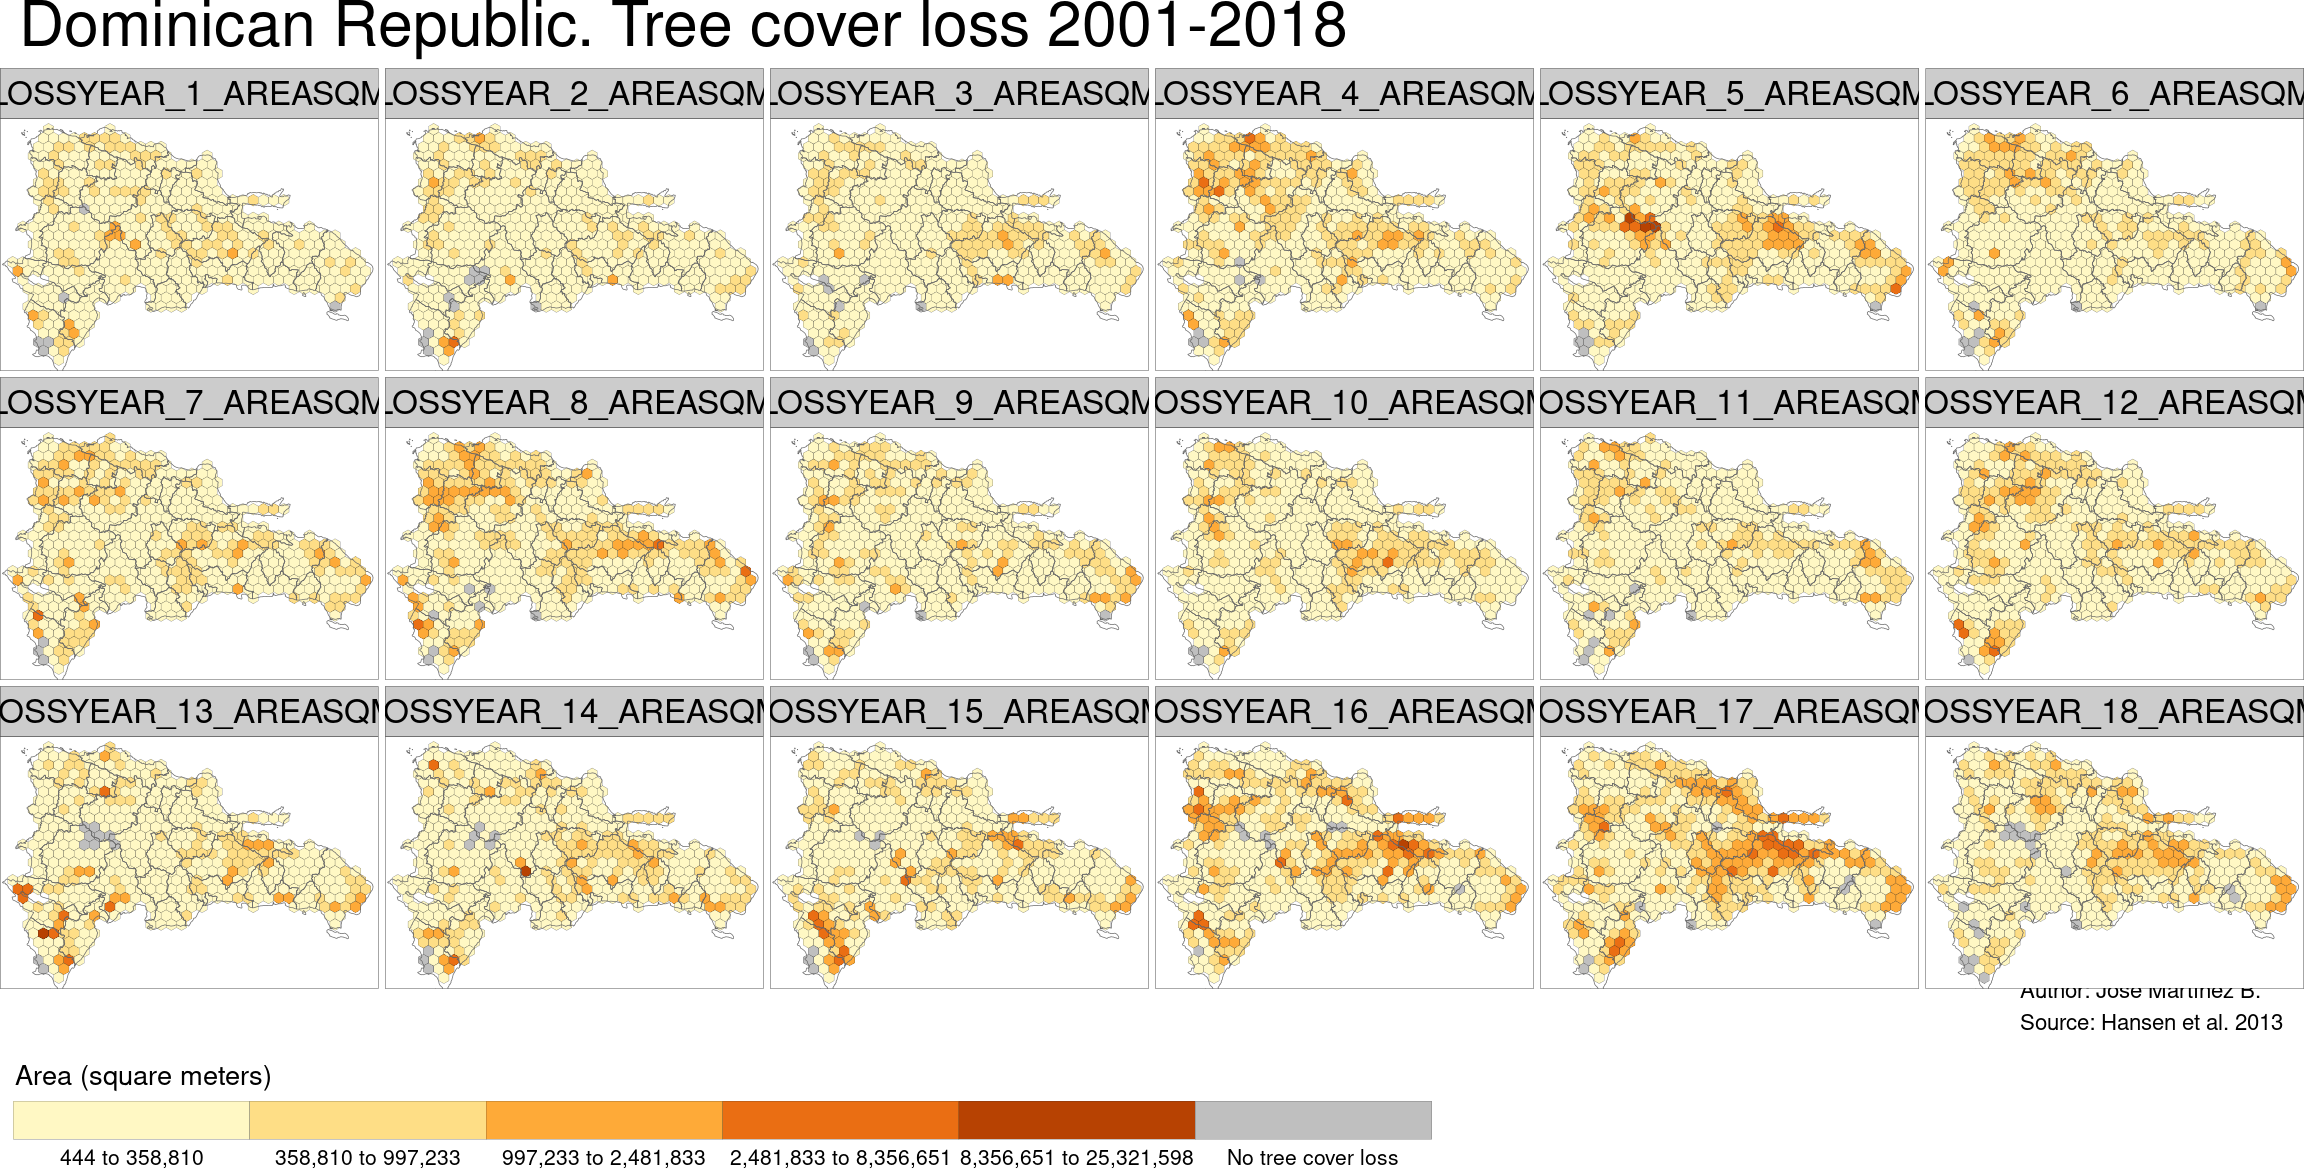
\includegraphics{img/data-download-preparation-eda/zonal-long-term-grid-5} \end{center}

\begin{Shaded}
\begin{Highlighting}[]
\CommentTok{\# * Loss per unit area (PUA). Provinces overlayed, single scale}
\NormalTok{grdzonal }\SpecialCharTok{\%\textgreater{}\%}\NormalTok{ dplyr}\SpecialCharTok{::}\FunctionTok{select}\NormalTok{(}\FunctionTok{matches}\NormalTok{(}\StringTok{\textquotesingle{}\^{}LOSSYEAR\_[1{-}9].*PUA.*\textquotesingle{}}\NormalTok{)) }\SpecialCharTok{\%\textgreater{}\%}
  \FunctionTok{replace}\NormalTok{(}\FunctionTok{is.na}\NormalTok{(.), }\DecValTok{0}\NormalTok{) }\SpecialCharTok{\%\textgreater{}\%} 
  \FunctionTok{gather}\NormalTok{(variable, value, }\SpecialCharTok{{-}}\NormalTok{geometry) }\SpecialCharTok{\%\textgreater{}\%}
  \FunctionTok{mutate}\NormalTok{(}\AttributeTok{variable =} \FunctionTok{factor}\NormalTok{(variable, }\AttributeTok{levels =} \FunctionTok{unique}\NormalTok{(variable))) }\SpecialCharTok{\%\textgreater{}\%} 
  \FunctionTok{tm\_shape}\NormalTok{() }\SpecialCharTok{+}
  \FunctionTok{tm\_fill}\NormalTok{(}\AttributeTok{col=}\StringTok{\textquotesingle{}value\textquotesingle{}}\NormalTok{, }\AttributeTok{palette =} \StringTok{"YlOrBr"}\NormalTok{, }\AttributeTok{size =} \FloatTok{0.1}\NormalTok{,}
          \AttributeTok{style =} \StringTok{\textquotesingle{}kmeans\textquotesingle{}}\NormalTok{, }\AttributeTok{legend.is.portrait =}\NormalTok{ F, }\AttributeTok{legend.format =} \FunctionTok{list}\NormalTok{(}\AttributeTok{digits =} \DecValTok{3}\NormalTok{, }\AttributeTok{text.separator =} \StringTok{\textquotesingle{}{-}\textquotesingle{}}\NormalTok{),}
          \AttributeTok{title =} \StringTok{\textquotesingle{}Per unit area loss\textquotesingle{}}\NormalTok{, }\AttributeTok{textNA =} \StringTok{"No tree cover loss"}\NormalTok{) }\SpecialCharTok{+}
  \FunctionTok{tm\_borders}\NormalTok{(}\AttributeTok{col =} \StringTok{\textquotesingle{}grey15\textquotesingle{}}\NormalTok{, }\AttributeTok{lwd =} \FloatTok{0.3}\NormalTok{) }\SpecialCharTok{+}
  \FunctionTok{tm\_facets}\NormalTok{(}\AttributeTok{by =} \StringTok{"variable"}\NormalTok{, }\AttributeTok{ncol =} \DecValTok{6}\NormalTok{, }\AttributeTok{nrow =} \DecValTok{3}\NormalTok{, }\AttributeTok{free.coords =} \ConstantTok{FALSE}\NormalTok{, }\AttributeTok{free.scales =} \ConstantTok{FALSE}\NormalTok{) }\SpecialCharTok{+}
  \FunctionTok{tm\_layout}\NormalTok{(}\AttributeTok{panel.label.size =} \DecValTok{3}\NormalTok{, }\AttributeTok{legend.title.size =} \DecValTok{2}\NormalTok{, }\AttributeTok{legend.text.size =} \FloatTok{0.8}\NormalTok{,}
            \AttributeTok{legend.outside.position =} \StringTok{"bottom"}\NormalTok{ , }\AttributeTok{legend.outside.size =}\NormalTok{ .}\DecValTok{1}\NormalTok{,}
            \AttributeTok{main.title =} \StringTok{\textquotesingle{}Dominican Republic. Tree cover loss 2001{-}2018\textquotesingle{}}\NormalTok{,}
            \AttributeTok{main.title.size =} \FloatTok{2.5}\NormalTok{, }\AttributeTok{attr.outside=}\ConstantTok{TRUE}\NormalTok{) }\SpecialCharTok{+} 
  \FunctionTok{tm\_credits}\NormalTok{(}\StringTok{\textquotesingle{}}\SpecialCharTok{\textbackslash{}n}\StringTok{Author: José Martínez B.}\SpecialCharTok{\textbackslash{}n}\StringTok{Source: Hansen et al. 2013\textquotesingle{}}\NormalTok{, }\AttributeTok{size =} \DecValTok{2}\NormalTok{) }\SpecialCharTok{+}
  \FunctionTok{tm\_shape}\NormalTok{(prov) }\SpecialCharTok{+} \FunctionTok{tm\_borders}\NormalTok{()}
\end{Highlighting}
\end{Shaded}

\begin{center}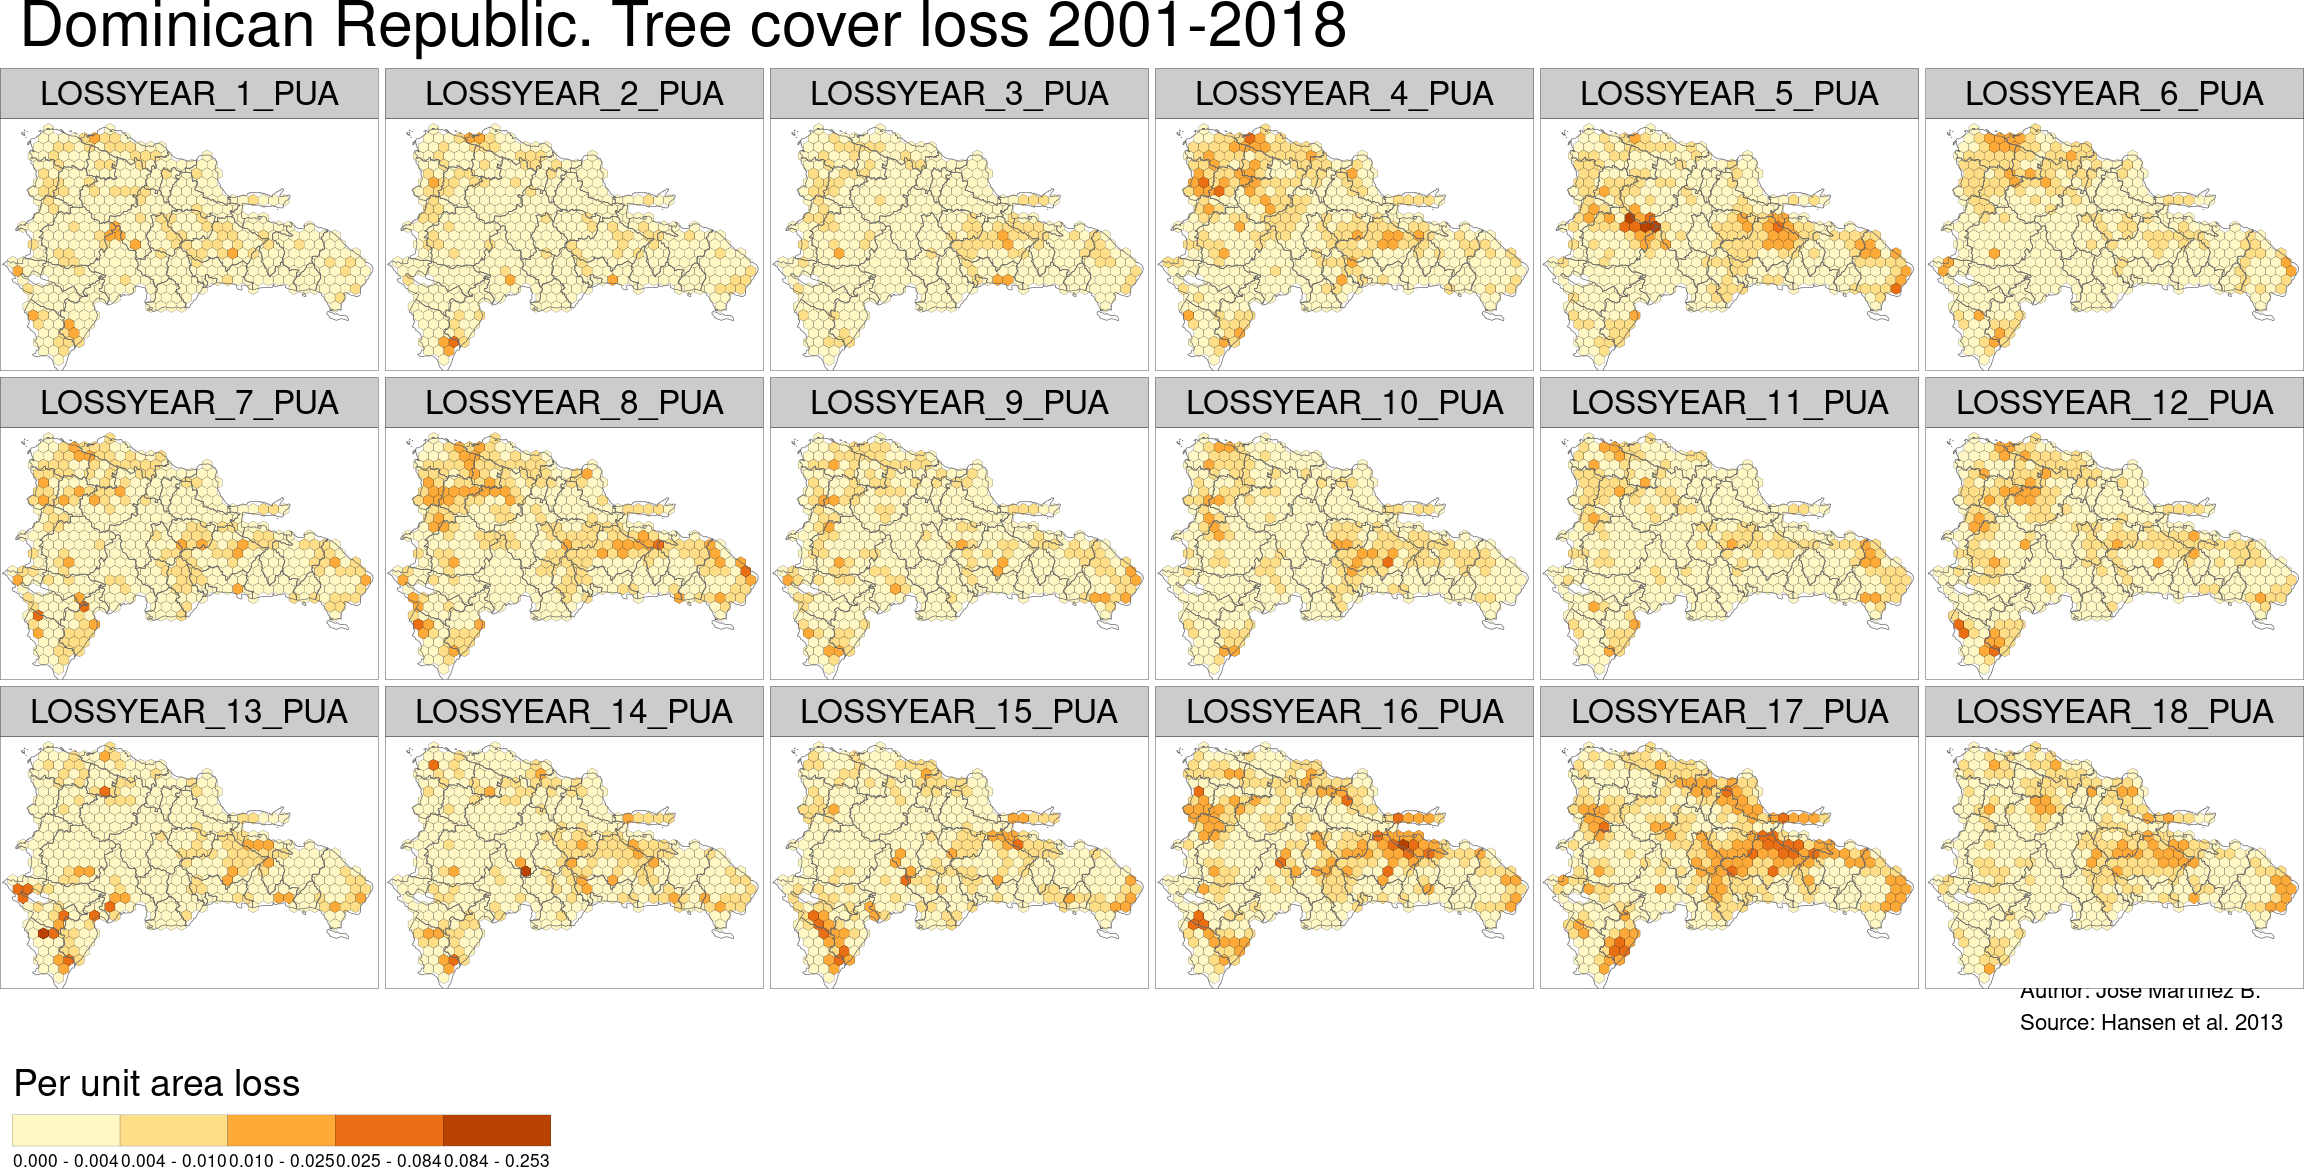
\includegraphics{img/data-download-preparation-eda/zonal-long-term-grid-6} \end{center}

\begin{Shaded}
\begin{Highlighting}[]

\CommentTok{\# Total loss 2001{-}2018}
\NormalTok{grdzonal }\SpecialCharTok{\%\textgreater{}\%} \FunctionTok{select}\NormalTok{(}\FunctionTok{matches}\NormalTok{(}\StringTok{\textquotesingle{}\^{}LOSS0118\textquotesingle{}}\NormalTok{)) }\SpecialCharTok{\%\textgreater{}\%} \FunctionTok{select}\NormalTok{(}\SpecialCharTok{{-}}\FunctionTok{matches}\NormalTok{(}\StringTok{\textquotesingle{}\textless{}NA\textgreater{}\textquotesingle{}}\NormalTok{)) }\SpecialCharTok{\%\textgreater{}\%} 
  \FunctionTok{gather}\NormalTok{(variable, value, }\SpecialCharTok{{-}}\NormalTok{geometry) }\SpecialCharTok{\%\textgreater{}\%}
  \FunctionTok{mutate}\NormalTok{(}\AttributeTok{variable =} \FunctionTok{factor}\NormalTok{(variable, }\AttributeTok{levels =} \FunctionTok{unique}\NormalTok{(variable))) }\SpecialCharTok{\%\textgreater{}\%} 
  \FunctionTok{tm\_shape}\NormalTok{() }\SpecialCharTok{+}
  \FunctionTok{tm\_fill}\NormalTok{(}\AttributeTok{col=}\StringTok{\textquotesingle{}value\textquotesingle{}}\NormalTok{, }\AttributeTok{palette =} \StringTok{"YlOrBr"}\NormalTok{, }\AttributeTok{size =} \FloatTok{0.1}\NormalTok{, }\AttributeTok{style =} \StringTok{\textquotesingle{}kmeans\textquotesingle{}}\NormalTok{) }\SpecialCharTok{+}
  \FunctionTok{tm\_borders}\NormalTok{(}\AttributeTok{col =} \StringTok{\textquotesingle{}grey15\textquotesingle{}}\NormalTok{, }\AttributeTok{lwd =} \FloatTok{0.3}\NormalTok{) }\SpecialCharTok{+}
  \FunctionTok{tm\_facets}\NormalTok{(}\AttributeTok{by =} \StringTok{"variable"}\NormalTok{, }\AttributeTok{ncol =} \DecValTok{2}\NormalTok{, }\AttributeTok{nrow =} \DecValTok{1}\NormalTok{, }\AttributeTok{free.coords =} \ConstantTok{FALSE}\NormalTok{, }\AttributeTok{free.scales =} \ConstantTok{TRUE}\NormalTok{) }\SpecialCharTok{+}
  \FunctionTok{tm\_layout}\NormalTok{(}\AttributeTok{panel.label.size =} \DecValTok{2}\NormalTok{, }\AttributeTok{legend.title.size =} \DecValTok{1}\NormalTok{, }\AttributeTok{legend.text.size =} \DecValTok{1}\NormalTok{) }\SpecialCharTok{+}
  \FunctionTok{tm\_shape}\NormalTok{(prov) }\SpecialCharTok{+} \FunctionTok{tm\_borders}\NormalTok{()}
\end{Highlighting}
\end{Shaded}

\begin{center}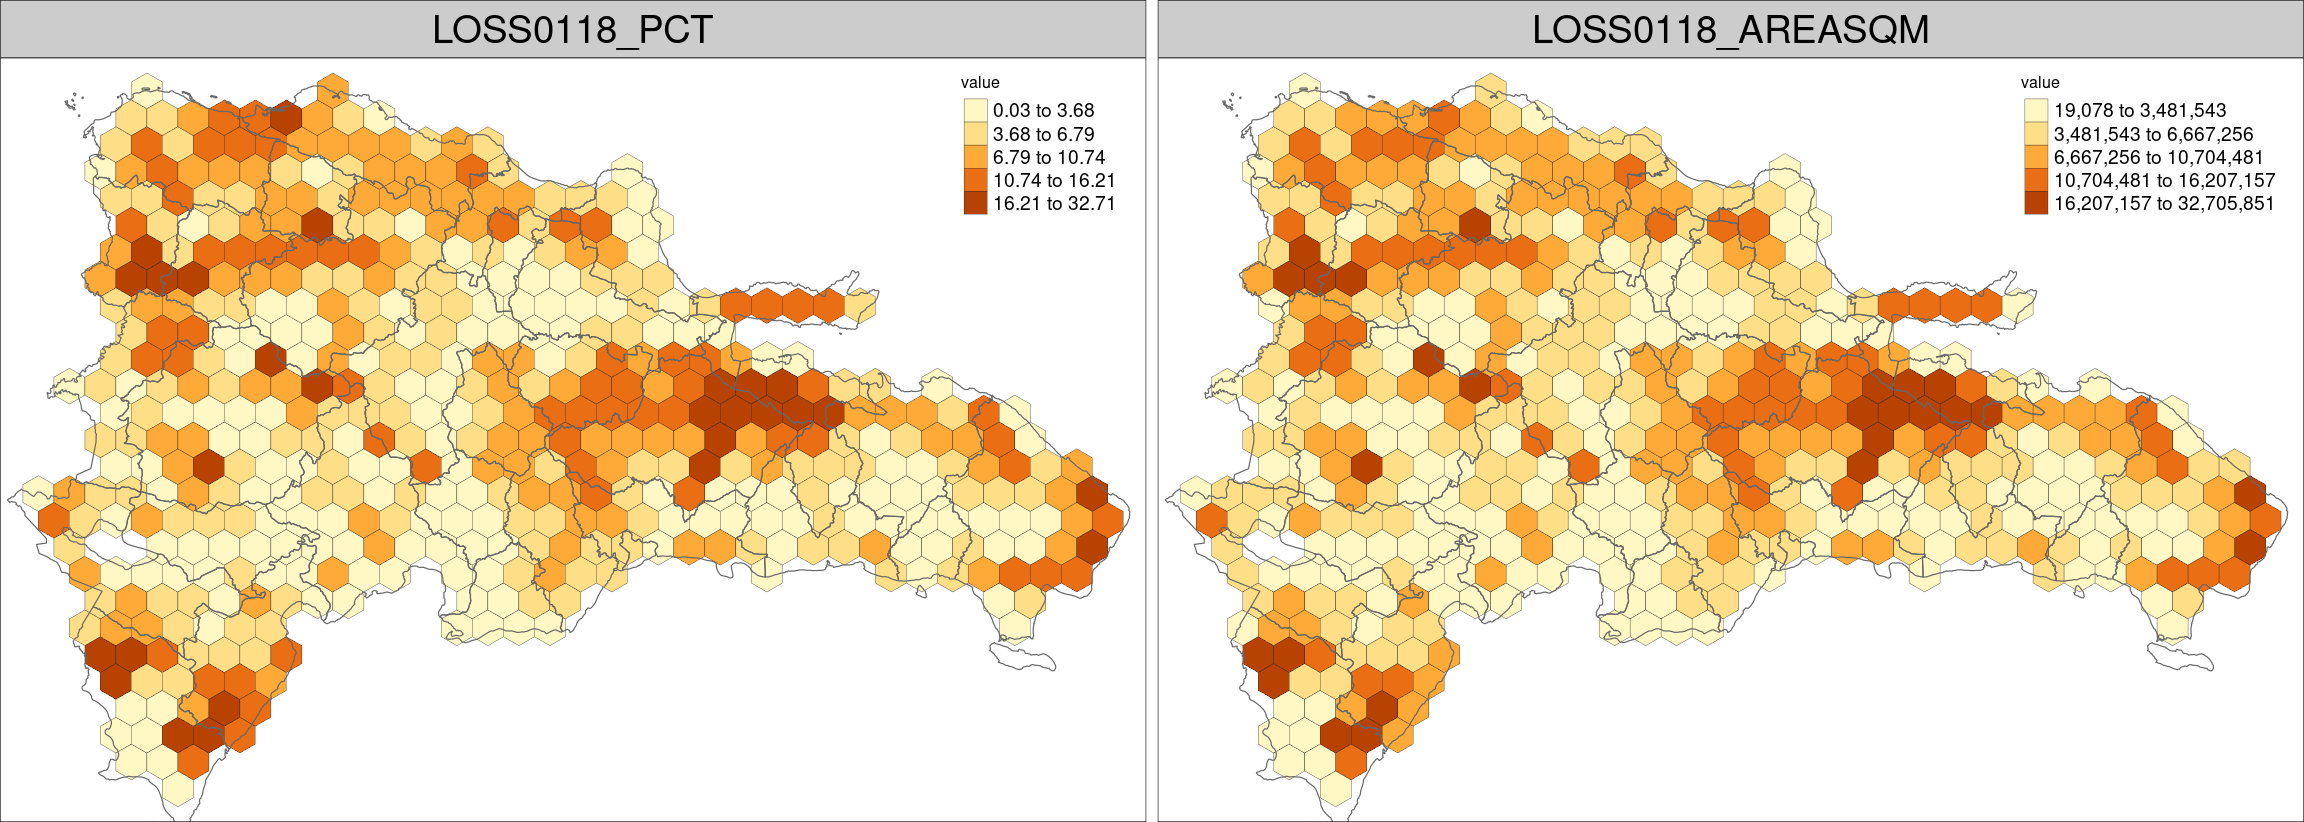
\includegraphics{img/data-download-preparation-eda/zonal-long-term-grid-7} \end{center}

\begin{verbatim}
## =====================================================
\end{verbatim}

\begin{center}\includegraphics{img/data-download-preparation-eda/zonal-long-term-grid-8} \end{center}

\begin{verbatim}
## ===========================
\end{verbatim}

\begin{center}\includegraphics{img/data-download-preparation-eda/zonal-long-term-grid-9} \end{center}

\begin{Shaded}
\begin{Highlighting}[]

\CommentTok{\# Total loss 2012{-}2018}
\NormalTok{grdzonal }\SpecialCharTok{\%\textgreater{}\%} \FunctionTok{select}\NormalTok{(}\FunctionTok{matches}\NormalTok{(}\StringTok{\textquotesingle{}\^{}LOSS1218\textquotesingle{}}\NormalTok{)) }\SpecialCharTok{\%\textgreater{}\%} \FunctionTok{select}\NormalTok{(}\SpecialCharTok{{-}}\FunctionTok{matches}\NormalTok{(}\StringTok{\textquotesingle{}\textless{}NA\textgreater{}\textquotesingle{}}\NormalTok{)) }\SpecialCharTok{\%\textgreater{}\%} 
  \FunctionTok{gather}\NormalTok{(variable, value, }\SpecialCharTok{{-}}\NormalTok{geometry) }\SpecialCharTok{\%\textgreater{}\%}
  \FunctionTok{mutate}\NormalTok{(}\AttributeTok{variable =} \FunctionTok{factor}\NormalTok{(variable, }\AttributeTok{levels =} \FunctionTok{unique}\NormalTok{(variable))) }\SpecialCharTok{\%\textgreater{}\%} 
  \FunctionTok{tm\_shape}\NormalTok{() }\SpecialCharTok{+}
    \FunctionTok{tm\_fill}\NormalTok{(}\AttributeTok{col=}\StringTok{\textquotesingle{}value\textquotesingle{}}\NormalTok{, }\AttributeTok{palette =} \StringTok{"YlOrBr"}\NormalTok{, }\AttributeTok{size =} \FloatTok{0.1}\NormalTok{, }\AttributeTok{style =} \StringTok{\textquotesingle{}kmeans\textquotesingle{}}\NormalTok{) }\SpecialCharTok{+}
    \FunctionTok{tm\_borders}\NormalTok{(}\AttributeTok{col =} \StringTok{\textquotesingle{}grey15\textquotesingle{}}\NormalTok{, }\AttributeTok{lwd =} \FloatTok{0.3}\NormalTok{) }\SpecialCharTok{+}
    \FunctionTok{tm\_facets}\NormalTok{(}\AttributeTok{by =} \StringTok{"variable"}\NormalTok{, }\AttributeTok{ncol =} \DecValTok{2}\NormalTok{, }\AttributeTok{nrow =} \DecValTok{1}\NormalTok{, }\AttributeTok{free.coords =} \ConstantTok{FALSE}\NormalTok{, }\AttributeTok{free.scales =} \ConstantTok{TRUE}\NormalTok{) }\SpecialCharTok{+}
    \FunctionTok{tm\_layout}\NormalTok{(}\AttributeTok{panel.label.size =} \DecValTok{2}\NormalTok{, }\AttributeTok{legend.title.size =} \DecValTok{1}\NormalTok{, }\AttributeTok{legend.text.size =} \DecValTok{1}\NormalTok{) }\SpecialCharTok{+}
  \FunctionTok{tm\_shape}\NormalTok{(prov) }\SpecialCharTok{+} \FunctionTok{tm\_borders}\NormalTok{()}
\end{Highlighting}
\end{Shaded}

\begin{center}\includegraphics{img/data-download-preparation-eda/zonal-long-term-grid-10} \end{center}

\begin{verbatim}
## =====================================================
\end{verbatim}

\begin{center}\includegraphics{img/data-download-preparation-eda/zonal-long-term-grid-11} \end{center}

\begin{verbatim}
## ===========================
\end{verbatim}

\begin{center}\includegraphics{img/data-download-preparation-eda/zonal-long-term-grid-12} \end{center}

\begin{Shaded}
\begin{Highlighting}[]

\CommentTok{\# Fires M6 and LOSS0118}
\NormalTok{grdzonal }\SpecialCharTok{\%\textgreater{}\%}\NormalTok{ dplyr}\SpecialCharTok{::}\FunctionTok{select}\NormalTok{(}\FunctionTok{matches}\NormalTok{(}\StringTok{\textquotesingle{}LOSS0118\_PUA\_PYR|NFIRESM6\_PSQKM\_PYR\textquotesingle{}}\NormalTok{)) }\SpecialCharTok{\%\textgreater{}\%} 
  \FunctionTok{replace}\NormalTok{(}\FunctionTok{is.na}\NormalTok{(.), }\DecValTok{0}\NormalTok{) }\SpecialCharTok{\%\textgreater{}\%} 
  \FunctionTok{gather}\NormalTok{(variable, value, }\SpecialCharTok{{-}}\NormalTok{geometry) }\SpecialCharTok{\%\textgreater{}\%}
  \FunctionTok{mutate}\NormalTok{(}\AttributeTok{variable =} \FunctionTok{factor}\NormalTok{(variable, }\AttributeTok{levels =} \FunctionTok{unique}\NormalTok{(variable))) }\SpecialCharTok{\%\textgreater{}\%} 
  \FunctionTok{tm\_shape}\NormalTok{() }\SpecialCharTok{+}
  \FunctionTok{tm\_fill}\NormalTok{(}\AttributeTok{col=}\StringTok{\textquotesingle{}value\textquotesingle{}}\NormalTok{, }\AttributeTok{palette =} \StringTok{"YlOrBr"}\NormalTok{, }\AttributeTok{size =} \FloatTok{0.1}\NormalTok{, }\AttributeTok{style =} \StringTok{\textquotesingle{}kmeans\textquotesingle{}}\NormalTok{) }\SpecialCharTok{+}
  \FunctionTok{tm\_borders}\NormalTok{(}\AttributeTok{col =} \StringTok{\textquotesingle{}grey15\textquotesingle{}}\NormalTok{, }\AttributeTok{lwd =} \FloatTok{0.3}\NormalTok{) }\SpecialCharTok{+}
  \FunctionTok{tm\_facets}\NormalTok{(}\AttributeTok{by =} \StringTok{"variable"}\NormalTok{, }\AttributeTok{ncol =} \DecValTok{2}\NormalTok{, }\AttributeTok{nrow =} \DecValTok{1}\NormalTok{, }\AttributeTok{free.coords =} \ConstantTok{FALSE}\NormalTok{, }\AttributeTok{free.scales =} \ConstantTok{TRUE}\NormalTok{) }\SpecialCharTok{+}
  \FunctionTok{tm\_layout}\NormalTok{(}\AttributeTok{panel.label.size =} \DecValTok{2}\NormalTok{, }\AttributeTok{legend.title.size =} \DecValTok{1}\NormalTok{, }\AttributeTok{legend.text.size =} \DecValTok{1}\NormalTok{) }\SpecialCharTok{+}
  \FunctionTok{tm\_shape}\NormalTok{(prov) }\SpecialCharTok{+} \FunctionTok{tm\_borders}\NormalTok{()}
\end{Highlighting}
\end{Shaded}

\begin{center}\includegraphics{img/data-download-preparation-eda/zonal-long-term-grid-13} \end{center}

\begin{Shaded}
\begin{Highlighting}[]

\CommentTok{\# Fires V1 and LOSS1218}
\NormalTok{grdzonal }\SpecialCharTok{\%\textgreater{}\%}\NormalTok{ dplyr}\SpecialCharTok{::}\FunctionTok{select}\NormalTok{(}\FunctionTok{matches}\NormalTok{(}\StringTok{\textquotesingle{}LOSS1218\_PUA\_PYR|NFIRESV1\_PSQKM\_PYR\textquotesingle{}}\NormalTok{)) }\SpecialCharTok{\%\textgreater{}\%} 
  \FunctionTok{replace}\NormalTok{(}\FunctionTok{is.na}\NormalTok{(.), }\DecValTok{0}\NormalTok{) }\SpecialCharTok{\%\textgreater{}\%} 
  \FunctionTok{gather}\NormalTok{(variable, value, }\SpecialCharTok{{-}}\NormalTok{geometry) }\SpecialCharTok{\%\textgreater{}\%}
  \FunctionTok{mutate}\NormalTok{(}\AttributeTok{variable =} \FunctionTok{factor}\NormalTok{(variable, }\AttributeTok{levels =} \FunctionTok{unique}\NormalTok{(variable))) }\SpecialCharTok{\%\textgreater{}\%} 
  \FunctionTok{tm\_shape}\NormalTok{() }\SpecialCharTok{+}
  \FunctionTok{tm\_fill}\NormalTok{(}\AttributeTok{col=}\StringTok{\textquotesingle{}value\textquotesingle{}}\NormalTok{, }\AttributeTok{palette =} \StringTok{"YlOrBr"}\NormalTok{, }\AttributeTok{size =} \FloatTok{0.1}\NormalTok{, }\AttributeTok{style =} \StringTok{\textquotesingle{}kmeans\textquotesingle{}}\NormalTok{) }\SpecialCharTok{+}
  \FunctionTok{tm\_borders}\NormalTok{(}\AttributeTok{col =} \StringTok{\textquotesingle{}grey15\textquotesingle{}}\NormalTok{, }\AttributeTok{lwd =} \FloatTok{0.3}\NormalTok{) }\SpecialCharTok{+}
  \FunctionTok{tm\_facets}\NormalTok{(}\AttributeTok{by =} \StringTok{"variable"}\NormalTok{, }\AttributeTok{ncol =} \DecValTok{2}\NormalTok{, }\AttributeTok{nrow =} \DecValTok{1}\NormalTok{, }\AttributeTok{free.coords =} \ConstantTok{FALSE}\NormalTok{, }\AttributeTok{free.scales =} \ConstantTok{TRUE}\NormalTok{) }\SpecialCharTok{+}
  \FunctionTok{tm\_layout}\NormalTok{(}\AttributeTok{panel.label.size =} \DecValTok{2}\NormalTok{, }\AttributeTok{legend.title.size =} \DecValTok{1}\NormalTok{, }\AttributeTok{legend.text.size =} \DecValTok{1}\NormalTok{) }\SpecialCharTok{+}
  \FunctionTok{tm\_shape}\NormalTok{(prov) }\SpecialCharTok{+} \FunctionTok{tm\_borders}\NormalTok{()}
\end{Highlighting}
\end{Shaded}

\begin{center}\includegraphics{img/data-download-preparation-eda/zonal-long-term-grid-14} \end{center}

\begin{Shaded}
\begin{Highlighting}[]

\CommentTok{\# Fires M6 and LOSS0118, fires V1 and LOSS1218}
\NormalTok{grdzonal }\SpecialCharTok{\%\textgreater{}\%}\NormalTok{ dplyr}\SpecialCharTok{::}\FunctionTok{select}\NormalTok{(}\FunctionTok{matches}\NormalTok{(}\StringTok{\textquotesingle{}LOSS1218\_PUA\_PYR|NFIRESV1\_PSQKM\_PYR|LOSS0118\_PUA\_PYR|NFIRESM6\_PSQKM\_PYR\textquotesingle{}}\NormalTok{)) }\SpecialCharTok{\%\textgreater{}\%} 
  \FunctionTok{replace}\NormalTok{(}\FunctionTok{is.na}\NormalTok{(.), }\DecValTok{0}\NormalTok{) }\SpecialCharTok{\%\textgreater{}\%} 
  \FunctionTok{gather}\NormalTok{(variable, value, }\SpecialCharTok{{-}}\NormalTok{geometry) }\SpecialCharTok{\%\textgreater{}\%}
  \FunctionTok{mutate}\NormalTok{(}\AttributeTok{variable =} \FunctionTok{factor}\NormalTok{(variable, }\AttributeTok{levels =} \FunctionTok{unique}\NormalTok{(variable))) }\SpecialCharTok{\%\textgreater{}\%} 
  \FunctionTok{tm\_shape}\NormalTok{() }\SpecialCharTok{+}
  \FunctionTok{tm\_fill}\NormalTok{(}\AttributeTok{col=}\StringTok{\textquotesingle{}value\textquotesingle{}}\NormalTok{, }\AttributeTok{palette =} \StringTok{"YlOrBr"}\NormalTok{, }\AttributeTok{size =} \FloatTok{0.1}\NormalTok{, }\AttributeTok{style =} \StringTok{\textquotesingle{}kmeans\textquotesingle{}}\NormalTok{) }\SpecialCharTok{+}
  \FunctionTok{tm\_borders}\NormalTok{(}\AttributeTok{col =} \StringTok{\textquotesingle{}grey15\textquotesingle{}}\NormalTok{, }\AttributeTok{lwd =} \FloatTok{0.3}\NormalTok{) }\SpecialCharTok{+}
  \FunctionTok{tm\_facets}\NormalTok{(}\AttributeTok{by =} \StringTok{"variable"}\NormalTok{, }\AttributeTok{ncol =} \DecValTok{2}\NormalTok{, }\AttributeTok{nrow =} \DecValTok{2}\NormalTok{, }\AttributeTok{free.coords =} \ConstantTok{FALSE}\NormalTok{, }\AttributeTok{free.scales =} \ConstantTok{TRUE}\NormalTok{) }\SpecialCharTok{+}
  \FunctionTok{tm\_layout}\NormalTok{(}\AttributeTok{panel.label.size =} \DecValTok{2}\NormalTok{, }\AttributeTok{legend.title.size =} \DecValTok{1}\NormalTok{, }\AttributeTok{legend.text.size =} \DecValTok{1}\NormalTok{) }\SpecialCharTok{+}
  \FunctionTok{tm\_shape}\NormalTok{(prov) }\SpecialCharTok{+} \FunctionTok{tm\_borders}\NormalTok{()}
\end{Highlighting}
\end{Shaded}

\begin{center}\includegraphics{img/data-download-preparation-eda/zonal-long-term-grid-15} \end{center}

\hypertarget{zonal-by-grid-used-in-the-annual-analytical-approach}{%
\subsection{Zonal, by grid used in the annual analytical
approach}\label{zonal-by-grid-used-in-the-annual-analytical-approach}}

\begin{Shaded}
\begin{Highlighting}[]
\NormalTok{hexsf }\OtherTok{\textless{}{-}} \FunctionTok{readRDS}\NormalTok{(}\StringTok{\textquotesingle{}out/honeycomb\_grid\_sf.RDS\textquotesingle{}}\NormalTok{)}
\FunctionTok{tm\_shape}\NormalTok{(cline) }\SpecialCharTok{+}
  \FunctionTok{tm\_fill}\NormalTok{(}\StringTok{\textquotesingle{}grey90\textquotesingle{}}\NormalTok{) }\SpecialCharTok{+}
  \FunctionTok{tm\_borders}\NormalTok{(}\StringTok{\textquotesingle{}black\textquotesingle{}}\NormalTok{) }\SpecialCharTok{+}
  \FunctionTok{tm\_shape}\NormalTok{(hexsf) }\SpecialCharTok{+}
  \FunctionTok{tm\_fill}\NormalTok{(}\StringTok{\textquotesingle{}white\textquotesingle{}}\NormalTok{, }\AttributeTok{alpha =} \FloatTok{0.4}\NormalTok{) }\SpecialCharTok{+} 
  \FunctionTok{tm\_borders}\NormalTok{(}\StringTok{\textquotesingle{}black\textquotesingle{}}\NormalTok{) }\SpecialCharTok{+}
  \FunctionTok{tm\_text}\NormalTok{(}\StringTok{\textquotesingle{}ENLACE\textquotesingle{}}\NormalTok{, }\AttributeTok{size =} \DecValTok{1}\NormalTok{, }\AttributeTok{shadow =}\NormalTok{ T)}
\end{Highlighting}
\end{Shaded}

\begin{center}\includegraphics{img/data-download-preparation-eda/zonal-annual-grid-1} \end{center}

\begin{Shaded}
\begin{Highlighting}[]

\CommentTok{\#Zonal statistics object}
\NormalTok{hexzonal }\OtherTok{\textless{}{-}} \FunctionTok{readRDS}\NormalTok{(}\StringTok{\textquotesingle{}out/hex\_zonal\_statistics.RDS\textquotesingle{}}\NormalTok{)}

\CommentTok{\# Patches of forest loss \textgreater{} 1 Ha}
\NormalTok{hexzonal }\SpecialCharTok{\%\textgreater{}\%} \FunctionTok{select}\NormalTok{(}\FunctionTok{matches}\NormalTok{(}\StringTok{\textquotesingle{}\^{}year.*loss1ha\_AREASQM\textquotesingle{}}\NormalTok{)) }\SpecialCharTok{\%\textgreater{}\%}
  \FunctionTok{rename\_at}\NormalTok{(}\FunctionTok{vars}\NormalTok{(}\FunctionTok{matches}\NormalTok{(}\StringTok{\textquotesingle{}\^{}year.*loss1ha\_AREASQM\textquotesingle{}}\NormalTok{)), }\FunctionTok{funs}\NormalTok{(}\FunctionTok{gsub}\NormalTok{(}\StringTok{\textquotesingle{}}\SpecialCharTok{\textbackslash{}\textbackslash{}}\StringTok{.loss1ha\_AREASQM\textquotesingle{}}\NormalTok{,}\StringTok{\textquotesingle{}\textquotesingle{}}\NormalTok{,.))) }\SpecialCharTok{\%\textgreater{}\%} 
  \FunctionTok{gather}\NormalTok{(variable, value, }\SpecialCharTok{{-}}\NormalTok{geometry) }\SpecialCharTok{\%\textgreater{}\%}
  \FunctionTok{mutate}\NormalTok{(}\AttributeTok{variable =} \FunctionTok{factor}\NormalTok{(variable, }\AttributeTok{levels =} \FunctionTok{unique}\NormalTok{(variable))) }\SpecialCharTok{\%\textgreater{}\%} 
  \FunctionTok{tm\_shape}\NormalTok{() }\SpecialCharTok{+}
  \FunctionTok{tm\_fill}\NormalTok{(}\AttributeTok{col=}\StringTok{\textquotesingle{}value\textquotesingle{}}\NormalTok{, }\AttributeTok{palette =} \StringTok{"YlOrBr"}\NormalTok{, }\AttributeTok{size =} \FloatTok{0.1}\NormalTok{,}
          \AttributeTok{style =} \StringTok{\textquotesingle{}kmeans\textquotesingle{}}\NormalTok{, }\AttributeTok{legend.is.portrait =}\NormalTok{ F, }\AttributeTok{title =} \StringTok{\textquotesingle{}Area (square meters)\textquotesingle{}}\NormalTok{,}
          \AttributeTok{textNA =} \StringTok{"No tree cover loss"}\NormalTok{) }\SpecialCharTok{+}
  \FunctionTok{tm\_borders}\NormalTok{(}\AttributeTok{col =} \StringTok{\textquotesingle{}grey15\textquotesingle{}}\NormalTok{, }\AttributeTok{lwd =} \FloatTok{0.3}\NormalTok{) }\SpecialCharTok{+}
  \FunctionTok{tm\_facets}\NormalTok{(}\AttributeTok{by =} \StringTok{"variable"}\NormalTok{, }\AttributeTok{ncol =} \DecValTok{6}\NormalTok{, }\AttributeTok{nrow =} \DecValTok{3}\NormalTok{, }\AttributeTok{free.coords =} \ConstantTok{FALSE}\NormalTok{, }\AttributeTok{free.scales =} \ConstantTok{FALSE}\NormalTok{) }\SpecialCharTok{+}
  \FunctionTok{tm\_layout}\NormalTok{(}\AttributeTok{panel.label.size =} \DecValTok{3}\NormalTok{, }\AttributeTok{legend.title.size =} \DecValTok{1}\NormalTok{, }\AttributeTok{legend.text.size =} \FloatTok{1.5}\NormalTok{,}
            \AttributeTok{legend.outside.position =} \StringTok{"bottom"}\NormalTok{ , }\AttributeTok{legend.outside.size =}\NormalTok{ .}\DecValTok{1}\NormalTok{,}
            \AttributeTok{main.title =} \StringTok{\textquotesingle{}Dominican Republic. Tree cover loss 2001{-}2018 within annual analytical approach hex grid\textquotesingle{}}\NormalTok{, }\AttributeTok{main.title.size =} \DecValTok{2}\NormalTok{, }\AttributeTok{attr.outside=}\ConstantTok{TRUE}\NormalTok{) }\SpecialCharTok{+} 
  \FunctionTok{tm\_credits}\NormalTok{(}\StringTok{\textquotesingle{}Author: José Martínez B.}\SpecialCharTok{\textbackslash{}n}\StringTok{Source: Hansen et al. 2013\textquotesingle{}}\NormalTok{, }\AttributeTok{size =} \FloatTok{1.5}\NormalTok{) }\SpecialCharTok{+}
  \FunctionTok{tm\_scale\_bar}\NormalTok{(}\AttributeTok{size =} \FloatTok{1.3}\NormalTok{) }\SpecialCharTok{+}
  \FunctionTok{tm\_shape}\NormalTok{(prov) }\SpecialCharTok{+} \FunctionTok{tm\_borders}\NormalTok{()}
\end{Highlighting}
\end{Shaded}

\begin{center}\includegraphics{img/data-download-preparation-eda/zonal-annual-grid-2} \end{center}

\begin{Shaded}
\begin{Highlighting}[]

\CommentTok{\# Fires M6}
\NormalTok{hexzonal }\SpecialCharTok{\%\textgreater{}\%} \FunctionTok{select}\NormalTok{(}\FunctionTok{matches}\NormalTok{(}\StringTok{\textquotesingle{}NFIRESM6\textquotesingle{}}\NormalTok{)) }\SpecialCharTok{\%\textgreater{}\%} \FunctionTok{select}\NormalTok{(}\SpecialCharTok{{-}}\FunctionTok{matches}\NormalTok{(}\StringTok{\textquotesingle{}\textless{}NA\textgreater{}\textquotesingle{}}\NormalTok{)) }\SpecialCharTok{\%\textgreater{}\%} 
  \FunctionTok{rename\_at}\NormalTok{(}\FunctionTok{vars}\NormalTok{(}\FunctionTok{matches}\NormalTok{(}\StringTok{\textquotesingle{}\^{}NFIRESM6\textquotesingle{}}\NormalTok{)), }\FunctionTok{funs}\NormalTok{(}\FunctionTok{gsub}\NormalTok{(}\StringTok{\textquotesingle{}\^{}NFIRESM6\_\textquotesingle{}}\NormalTok{,}\StringTok{\textquotesingle{}\textquotesingle{}}\NormalTok{,.))) }\SpecialCharTok{\%\textgreater{}\%} 
  \FunctionTok{gather}\NormalTok{(variable, value, }\SpecialCharTok{{-}}\NormalTok{geometry) }\SpecialCharTok{\%\textgreater{}\%}
  \FunctionTok{mutate}\NormalTok{(}\AttributeTok{variable =} \FunctionTok{factor}\NormalTok{(variable, }\AttributeTok{levels =} \FunctionTok{unique}\NormalTok{(variable))) }\SpecialCharTok{\%\textgreater{}\%} 
  \FunctionTok{tm\_shape}\NormalTok{() }\SpecialCharTok{+}
  \FunctionTok{tm\_fill}\NormalTok{(}\AttributeTok{col=}\StringTok{\textquotesingle{}value\textquotesingle{}}\NormalTok{, }\AttributeTok{palette =} \StringTok{"YlOrBr"}\NormalTok{, }\AttributeTok{size =} \FloatTok{0.1}\NormalTok{,}
          \AttributeTok{style =} \StringTok{\textquotesingle{}kmeans\textquotesingle{}}\NormalTok{, }\AttributeTok{legend.is.portrait =}\NormalTok{ F, }\AttributeTok{title =} \StringTok{\textquotesingle{}Number of fires/hotspots at \textless{}2.5 km from forest loss\textquotesingle{}}\NormalTok{,}
          \AttributeTok{textNA =} \StringTok{"No fires/hotspots"}\NormalTok{) }\SpecialCharTok{+}
  \FunctionTok{tm\_borders}\NormalTok{(}\AttributeTok{col =} \StringTok{\textquotesingle{}grey15\textquotesingle{}}\NormalTok{, }\AttributeTok{lwd =} \FloatTok{0.3}\NormalTok{) }\SpecialCharTok{+}
  \FunctionTok{tm\_facets}\NormalTok{(}\AttributeTok{by =} \StringTok{"variable"}\NormalTok{, }\AttributeTok{ncol =} \DecValTok{6}\NormalTok{, }\AttributeTok{nrow =} \DecValTok{3}\NormalTok{, }\AttributeTok{free.coords =} \ConstantTok{FALSE}\NormalTok{, }\AttributeTok{free.scales =} \ConstantTok{FALSE}\NormalTok{) }\SpecialCharTok{+}
  \FunctionTok{tm\_layout}\NormalTok{(}\AttributeTok{panel.label.size =} \DecValTok{3}\NormalTok{, }\AttributeTok{legend.title.size =} \DecValTok{1}\NormalTok{, }\AttributeTok{legend.text.size =} \FloatTok{1.5}\NormalTok{,}
            \AttributeTok{legend.outside.position =} \StringTok{"bottom"}\NormalTok{ , }\AttributeTok{legend.outside.size =}\NormalTok{ .}\DecValTok{1}\NormalTok{,}
            \AttributeTok{main.title =} \StringTok{\textquotesingle{}Dominican Republic. Number of selected fires/hotspots detected by MODIS, 2001{-}2018,  within annual analytical approach hex grid\textquotesingle{}}\NormalTok{,}
            \AttributeTok{main.title.size =} \DecValTok{2}\NormalTok{, }\AttributeTok{attr.outside=}\ConstantTok{TRUE}\NormalTok{) }\SpecialCharTok{+} 
  \FunctionTok{tm\_credits}\NormalTok{(}\StringTok{\textquotesingle{}Author: José Martínez B.}\SpecialCharTok{\textbackslash{}n}\StringTok{Source: NASA/FIRMS\textquotesingle{}}\NormalTok{, }\AttributeTok{size =} \FloatTok{1.5}\NormalTok{) }\SpecialCharTok{+}
  \FunctionTok{tm\_scale\_bar}\NormalTok{(}\AttributeTok{size =} \FloatTok{1.3}\NormalTok{) }\SpecialCharTok{+}
  \FunctionTok{tm\_shape}\NormalTok{(prov) }\SpecialCharTok{+} \FunctionTok{tm\_borders}\NormalTok{()}
\end{Highlighting}
\end{Shaded}

\begin{center}\includegraphics{img/data-download-preparation-eda/zonal-annual-grid-3} \end{center}

\begin{Shaded}
\begin{Highlighting}[]

\CommentTok{\# Fires V1}
\NormalTok{hexzonal }\SpecialCharTok{\%\textgreater{}\%} \FunctionTok{select}\NormalTok{(}\FunctionTok{matches}\NormalTok{(}\StringTok{\textquotesingle{}NFIRESV1\textquotesingle{}}\NormalTok{)) }\SpecialCharTok{\%\textgreater{}\%} \FunctionTok{select}\NormalTok{(}\SpecialCharTok{{-}}\FunctionTok{matches}\NormalTok{(}\StringTok{\textquotesingle{}\textless{}NA\textgreater{}\textquotesingle{}}\NormalTok{)) }\SpecialCharTok{\%\textgreater{}\%} 
  \FunctionTok{rename\_at}\NormalTok{(}\FunctionTok{vars}\NormalTok{(}\FunctionTok{matches}\NormalTok{(}\StringTok{\textquotesingle{}\^{}NFIRESV1\textquotesingle{}}\NormalTok{)), }\FunctionTok{funs}\NormalTok{(}\FunctionTok{gsub}\NormalTok{(}\StringTok{\textquotesingle{}\^{}NFIRESV1\_\textquotesingle{}}\NormalTok{,}\StringTok{\textquotesingle{}\textquotesingle{}}\NormalTok{,.))) }\SpecialCharTok{\%\textgreater{}\%} 
  \FunctionTok{gather}\NormalTok{(variable, value, }\SpecialCharTok{{-}}\NormalTok{geometry) }\SpecialCharTok{\%\textgreater{}\%}
  \FunctionTok{mutate}\NormalTok{(}\AttributeTok{variable =} \FunctionTok{factor}\NormalTok{(variable, }\AttributeTok{levels =} \FunctionTok{unique}\NormalTok{(variable))) }\SpecialCharTok{\%\textgreater{}\%} 
  \FunctionTok{tm\_shape}\NormalTok{() }\SpecialCharTok{+}
  \FunctionTok{tm\_fill}\NormalTok{(}\AttributeTok{col=}\StringTok{\textquotesingle{}value\textquotesingle{}}\NormalTok{, }\AttributeTok{palette =} \StringTok{"YlOrBr"}\NormalTok{, }\AttributeTok{size =} \FloatTok{0.1}\NormalTok{,}
          \AttributeTok{style =} \StringTok{\textquotesingle{}kmeans\textquotesingle{}}\NormalTok{, }\AttributeTok{legend.is.portrait =}\NormalTok{ F, }\AttributeTok{title =} \StringTok{\textquotesingle{}Number of fires/hotspots at \textless{}2.5 km from forest loss\textquotesingle{}}\NormalTok{,}
          \AttributeTok{textNA =} \StringTok{"No tree cover loss"}\NormalTok{) }\SpecialCharTok{+}
  \FunctionTok{tm\_borders}\NormalTok{(}\AttributeTok{col =} \StringTok{\textquotesingle{}grey15\textquotesingle{}}\NormalTok{, }\AttributeTok{lwd =} \FloatTok{0.3}\NormalTok{) }\SpecialCharTok{+}
  \FunctionTok{tm\_facets}\NormalTok{(}\AttributeTok{by =} \StringTok{"variable"}\NormalTok{, }\AttributeTok{ncol =} \DecValTok{4}\NormalTok{, }\AttributeTok{nrow =} \DecValTok{2}\NormalTok{, }\AttributeTok{free.coords =} \ConstantTok{FALSE}\NormalTok{, }\AttributeTok{free.scales =} \ConstantTok{FALSE}\NormalTok{) }\SpecialCharTok{+}
  \FunctionTok{tm\_layout}\NormalTok{(}\AttributeTok{panel.label.size =} \DecValTok{3}\NormalTok{, }\AttributeTok{legend.title.size =} \DecValTok{1}\NormalTok{, }\AttributeTok{legend.text.size =} \FloatTok{1.5}\NormalTok{,}
            \AttributeTok{legend.outside.position =} \StringTok{"bottom"}\NormalTok{ , }\AttributeTok{legend.outside.size =}\NormalTok{ .}\DecValTok{1}\NormalTok{,}
            \AttributeTok{main.title =} \StringTok{\textquotesingle{}Dominican Republic. Number of selected fires/hotspots detected by VIIRS, 2001{-}2018,  within annual analytical approach hex grid\textquotesingle{}}\NormalTok{,}
            \AttributeTok{main.title.size =} \DecValTok{2}\NormalTok{, }\AttributeTok{attr.outside=}\ConstantTok{TRUE}\NormalTok{) }\SpecialCharTok{+} 
  \FunctionTok{tm\_credits}\NormalTok{(}\StringTok{\textquotesingle{}Author: José Martínez B.}\SpecialCharTok{\textbackslash{}n}\StringTok{Source: NASA/FIRMS\textquotesingle{}}\NormalTok{, }\AttributeTok{size =} \FloatTok{1.5}\NormalTok{) }\SpecialCharTok{+}
  \FunctionTok{tm\_scale\_bar}\NormalTok{(}\AttributeTok{size =} \FloatTok{1.3}\NormalTok{) }\SpecialCharTok{+}
  \FunctionTok{tm\_shape}\NormalTok{(prov) }\SpecialCharTok{+} \FunctionTok{tm\_borders}\NormalTok{()}
\end{Highlighting}
\end{Shaded}

\begin{center}\includegraphics{img/data-download-preparation-eda/zonal-annual-grid-4} \end{center}

\begin{Shaded}
\begin{Highlighting}[]

\CommentTok{\# Patches of forest loss \textless{} 1 ha}
\NormalTok{hexzonal }\SpecialCharTok{\%\textgreater{}\%} \FunctionTok{select}\NormalTok{(}\FunctionTok{matches}\NormalTok{(}\StringTok{\textquotesingle{}NCLUMPSSMALLER1HA\_\textquotesingle{}}\NormalTok{)) }\SpecialCharTok{\%\textgreater{}\%} 
  \FunctionTok{rename\_at}\NormalTok{(}\FunctionTok{vars}\NormalTok{(}\FunctionTok{matches}\NormalTok{(}\StringTok{\textquotesingle{}\^{}NCLUMPSSMALLER1HA\_\textquotesingle{}}\NormalTok{)), }\FunctionTok{funs}\NormalTok{(}\FunctionTok{gsub}\NormalTok{(}\StringTok{\textquotesingle{}\^{}NCLUMPSSMALLER1HA\_\textquotesingle{}}\NormalTok{,}\StringTok{\textquotesingle{}\textquotesingle{}}\NormalTok{,.))) }\SpecialCharTok{\%\textgreater{}\%} 
  \FunctionTok{gather}\NormalTok{(variable, value, }\SpecialCharTok{{-}}\NormalTok{geometry) }\SpecialCharTok{\%\textgreater{}\%}
  \FunctionTok{mutate}\NormalTok{(}\AttributeTok{variable =} \FunctionTok{factor}\NormalTok{(variable, }\AttributeTok{levels =} \FunctionTok{unique}\NormalTok{(variable))) }\SpecialCharTok{\%\textgreater{}\%} 
  \FunctionTok{tm\_shape}\NormalTok{() }\SpecialCharTok{+}
  \FunctionTok{tm\_fill}\NormalTok{(}\AttributeTok{col=}\StringTok{\textquotesingle{}value\textquotesingle{}}\NormalTok{, }\AttributeTok{palette =} \StringTok{"YlOrBr"}\NormalTok{, }\AttributeTok{size =} \FloatTok{0.1}\NormalTok{,}
          \AttributeTok{style =} \StringTok{\textquotesingle{}kmeans\textquotesingle{}}\NormalTok{, }\AttributeTok{legend.is.portrait =}\NormalTok{ F, }\AttributeTok{title =} \StringTok{\textquotesingle{}Number of clumps\textquotesingle{}}\NormalTok{,}
          \AttributeTok{textNA =} \StringTok{"No tree cover loss"}\NormalTok{) }\SpecialCharTok{+}
  \FunctionTok{tm\_borders}\NormalTok{(}\AttributeTok{col =} \StringTok{\textquotesingle{}grey15\textquotesingle{}}\NormalTok{, }\AttributeTok{lwd =} \FloatTok{0.3}\NormalTok{) }\SpecialCharTok{+}
  \FunctionTok{tm\_facets}\NormalTok{(}\AttributeTok{by =} \StringTok{"variable"}\NormalTok{, }\AttributeTok{ncol =} \DecValTok{6}\NormalTok{, }\AttributeTok{nrow =} \DecValTok{3}\NormalTok{, }\AttributeTok{free.coords =} \ConstantTok{FALSE}\NormalTok{, }\AttributeTok{free.scales =} \ConstantTok{FALSE}\NormalTok{) }\SpecialCharTok{+}
  \FunctionTok{tm\_layout}\NormalTok{(}\AttributeTok{panel.label.size =} \DecValTok{3}\NormalTok{, }\AttributeTok{legend.title.size =} \DecValTok{1}\NormalTok{, }\AttributeTok{legend.text.size =} \FloatTok{1.5}\NormalTok{,}
            \AttributeTok{legend.outside.position =} \StringTok{"bottom"}\NormalTok{ , }\AttributeTok{legend.outside.size =}\NormalTok{ .}\DecValTok{1}\NormalTok{,}
            \AttributeTok{main.title =} \StringTok{\textquotesingle{}Dominican Republic. Number of clumps of forest loss \textless{}1ha,  within annual analyticial approach hex grid\textquotesingle{}}\NormalTok{,}
            \AttributeTok{main.title.size =} \DecValTok{2}\NormalTok{, }\AttributeTok{attr.outside=}\ConstantTok{TRUE}\NormalTok{) }\SpecialCharTok{+} 
  \FunctionTok{tm\_credits}\NormalTok{(}\StringTok{\textquotesingle{}Author: José Martínez B.}\SpecialCharTok{\textbackslash{}n}\StringTok{Source: Hansen et al., 2013\textquotesingle{}}\NormalTok{, }\AttributeTok{size =} \FloatTok{1.5}\NormalTok{) }\SpecialCharTok{+}
  \FunctionTok{tm\_scale\_bar}\NormalTok{(}\AttributeTok{size =} \FloatTok{1.3}\NormalTok{) }\SpecialCharTok{+}
  \FunctionTok{tm\_shape}\NormalTok{(prov) }\SpecialCharTok{+} \FunctionTok{tm\_borders}\NormalTok{()}
\end{Highlighting}
\end{Shaded}

\begin{center}\includegraphics{img/data-download-preparation-eda/zonal-annual-grid-5} \end{center}

\hypertarget{references}{%
\section*{References}\label{references}}
\addcontentsline{toc}{section}{References}

\hypertarget{refs}{}
\begin{CSLReferences}{1}{0}
\leavevmode\hypertarget{ref-hansen2013high}{}%
Hansen, M. C., Potapov, P. V., Moore, R., Hancher, M., Turubanova, S.,
Tyukavina, A., \ldots{} others. (2013). High-resolution global maps of
21st-century forest cover change. \emph{Science}, \emph{342}(6160),
850--853.

\leavevmode\hypertarget{ref-martinez2021forest}{}%
Martínez Batlle, J. R. (2021). {Forest loss and fire in the Dominican
Republic during the 21st Century}. \emph{bioRxiv}.
\url{https://doi.org/10.1101/2021.06.15.448604}

\leavevmode\hypertarget{ref-one2015datos}{}%
Oficina Nacional de Estadística -ONE-. (2015). \emph{Datos
georreferenciados}.
\url{https://www.one.gob.do/informaciones-cartograficas/shapefiles}.

\leavevmode\hypertarget{ref-unep2021protected}{}%
UNEP-WCMC and IUCN. (October 2021). \emph{{Protected Planet: The World
Database on Protected Areas (WDPA) and World Database on Other Effective
Area-based Conservation Measures (WD-OECM) {[}Online{]}}}.
\url{www.protectedplanet.net}; {Cambridge, UK: UNEP-WCMC and IUCN.}

\end{CSLReferences}




\newpage
\singlespacing 
\end{document}
